% paper.tex —— FGIB 论文主文件（intro / method / 部分实验）
% 以 template.tex 为模版。编译需要 ICLR 2027 官方样式包：
%   iclr2027_conference.sty, iclr2027_conference.bst
% 参考文献用内联 thebibliography（natbib author-year 格式），无需 bibtex。
% 附录 % fgib_theory.tex —— FGIB 完整理论推导（四个问题的证明 + FGIB 机制的证明）
% 本文件合并自 fgib_ceb_collapse.tex / fgib_degeneration.tex / fgib_bound.tex / fgib_linear.tex，
% 原四文件可删除；全部标签名保持不变，fgib_intro.tex / fgib_method.tex 的 \ref 不受影响。
% 用法：\usepackage{amsmath,amssymb,amsthm}，正文处 % fgib_theory.tex —— FGIB 完整理论推导（四个问题的证明 + FGIB 机制的证明）
% 本文件合并自 fgib_ceb_collapse.tex / fgib_degeneration.tex / fgib_bound.tex / fgib_linear.tex，
% 原四文件可删除；全部标签名保持不变，fgib_intro.tex / fgib_method.tex 的 \ref 不受影响。
% 用法：\usepackage{amsmath,amssymb,amsthm}，正文处 % fgib_theory.tex —— FGIB 完整理论推导（四个问题的证明 + FGIB 机制的证明）
% 本文件合并自 fgib_ceb_collapse.tex / fgib_degeneration.tex / fgib_bound.tex / fgib_linear.tex，
% 原四文件可删除；全部标签名保持不变，fgib_intro.tex / fgib_method.tex 的 \ref 不受影响。
% 用法：\usepackage{amsmath,amssymb,amsthm}，正文处 \input{fgib_theory.tex}。
% 记号沿用 Fischer (2020)、Kolchinsky & Tracey (2019, Caveats)、Kolchinsky et al. (2017, NIB)、
% Alemi et al. (2017, VIB)。
%
% 核心结论（FGIB 论文问题陈述与解法）：
% 第一部分（四条失效通道）：
%   P1 退化继承（死旋钮）：CEB ≡ IB(β=1+γ>1)，确定性场景下所有 γ>0 的唯一最优解钉在角点，
%      γ 扫不出任何中间点（SIB Caveat 1 的退化半区，经 β'=1/(1+γ)∈(0,1) 映射）。
%      该角点恰是 CEB 自己的 MNI 目标，rem:mni 正面处理这一反驳；
%   P2 证书盲视 + 1:β 交换率：T_α 流形上 ReX 恒为 0（证书对标签保留量完全盲视），
%      且目标以 1 nat 标签信息 ↔ β nat 认证残差的比率交换；
%   P3 方差竞赛：KL 两侧皆可训练，分类项压 σ→0、钳位处退化为权重 e^{10} 的均值匹配。
%      (ii)(iii) 是受力方向分析而非收敛证明，且可实测（rem:p3-status）；
%   P4 对象错位：两种方法的界都只界住各自的含噪码，都不界住确定性连续推理表示的残差
%      （后者为 +∞）。差别是结构性的（噪声在不在推理路径上），不是紧度排序。
% 第二部分（FGIB 机制，以及它没能关闭的通道）：
%   M1 等价性：旁路 = 固定 A 下作用在 h+已知噪声上的 CEB 瓶颈（逐步成立，非全程固定参考）；
%   M2 扫参：固定分类器尺度 c 时 L_β(s)=CE(s)+(β/2)(s−a)² 严格凸、每 β 唯一内点、曲线严格凹；
%      c 自由时下确界对所有 β 均为 0（rem:c-scale，给出权重归一化分类器的架构修法）；
%   M3 证书：gap 恒等式 + 矩匹配 + 固定编码器下的值排序；固定参考的力持续性成立，
%      但侧头 A 是推理无关的第二个自由方（rem:A-channel），构成未关闭的通道。
%
% 修订记录（第二轮）：理论/实现分层后统一引入锚点方差 τ²（先验 N(a v_y, τ²I)，默认 τ²=1，
% 后验方差最优 σ²*=τ²，σ_p 为公共方差记号；point-anchor 极限统一写为 τ→0）；理论旁路固定为
% 可逆线性头 T(h)=Ah（实现用带 bias 的 nn.Linear 近似，见理论-代码分层 caveat）；
% 明确 sweep 证明的是对齐族上 KL–CE surrogate 曲线（rem:surrogate），不是 IB 互信息曲线；
% 无穷互信息结论统一挂靠分布性 standing assumption；rem:c-scale 的架构修法收紧为
% 固定温度 cosine 分类器（weight decay 只缓解不发散）；a=0 退化点、条件数表述、
% 梯度消失条件、row-space 表述等小项修正。
%
% 修订记录（第一轮）：删除三处错误论断——(1) P3 原称 ReX≈0 时 I(X;Z|Y) 发散，与 gap 恒等式矛盾；
% (2) prop:object(c) 原称 FGIB 的界"更紧/唯一有效"，由 DPI 不成立；(3) prop:conditioning(iii)
% 原从 Gram 恒等式推出条件数为 1，有反例。修正 P2 的换算、Caveat 2 的主张、rem:frame 的
% A^T/V^T、mu_head 的仿射与非推理路径身份。未证结论统一收入 sec:limits。

\newtheorem{lemma}{Lemma}
\newtheorem{proposition}{Proposition}
\newtheorem{remark}{Remark}

% =====================================================================
\section*{Part I. The four failure channels of the conditional bottleneck}
% =====================================================================

\textbf{Notation.}
$X$ is the input and $Y$ the label with $K$ classes; the encoder induces the Markov chain
$Y - X - Z$. The \emph{deterministic scenario} is $Y = f(X)$ ($H(Y|X) = 0$). Following
Fischer (2020), we write the MNI point $I(X;Y) = I(X;Z) = I(Y;Z)$ (Eq.~1), the
chain-rule identity $I(X;Z|Y) = I(X;Z) - I(Y;Z)$ (Eq.~4), the CEB objective
$\mathrm{CEB} \equiv \min_Z I(X;Z|Y) - \gamma I(Y;Z)$ (Eq.~5), the IB objective
$\mathrm{IB} \equiv \min_Z I(X;Z) - \beta_{\mathrm{IB}} I(Y;Z)$ (Eq.~16), the
variational objective
$\mathrm{VCEB} \equiv \min_{e,b,c} \langle \log e(z|x)\rangle - \langle \log b(z|y)\rangle
- \gamma \langle \log c(y|z)\rangle$ (Eq.~15), and the residual certificate
$\mathrm{ReX} \equiv \langle \log e(z|x)\rangle - \langle \log b(z|y)\rangle
\ge I(X;Z|Y)$ (Eq.~20), where $b(z|y)$ is a \emph{trainable} backward encoder (we write
$q(z|x)$ for Fischer's encoder $e(z|x)$; the two notations are interchangeable
throughout). In the loss convention $\mathrm{CE} + \beta\,\mathrm{KL}$ used throughout, the weights are
$\beta = 1/\gamma$ and $\beta_{\mathrm{IB}} = 1 + \gamma = 1 + 1/\beta$. Following
Kolchinsky \& Tracey (2019), we write the IB curve $F(r)$ (their Eq.~1), the IB
Lagrangian $L^{\mathrm{IB}}_\beta = I(Y;T) - \beta I(X;T)$ (their Eq.~2), the
DPI-saturating manifold $T_\alpha := B_\alpha \cdot Y$ (their Eq.~6), the bound
$L^{\mathrm{IB}}_\beta \le (1-\beta)H(Y)$ (their Eq.~7), and their footnote~4 (the
$\beta > 1$ regime of trivial maximizers). The variational objects are
\begin{align*}
R &= \mathbb{E}\big[\operatorname{KL}(q(z|x)\,\|\,m(z))\big] \ge I(X;Z)
&&\text{(VIB rate, marginal prior $m$; Fischer Eq.~19, Alemi et al.\ Eq.~14)} \\
\mathrm{ReX} &= \mathbb{E}\big[\operatorname{KL}(q(z|x)\,\|\,b_\theta(z|y))\big]
\ge I(X;Z|Y)
&&\text{(CEB residual; Fischer Eq.~20)} \\
\widehat I &= -\frac{1}{N}\sum_i \ln\Big[\frac{1}{N}\sum_j
e^{-\|f_i-f_j\|^2/(2\sigma^2)}\Big] \ge I(X;M)
&&\text{(NIB, non-parametric; Eq.~16, the homoscedastic case of Eq.~10)} \\
\mathrm{ReX}_F &= \mathbb{E}\big[\operatorname{KL}(q(z|x)\,\|\,r(z|y))\big]
\ge I(X;Z|Y)
&&\text{(FGIB, fixed anchor)}
\end{align*}
(Fischer 2020, Eqs.~18--20; Alemi et al.\ 2017, Eq.~14; Kolchinsky et al.\ 2017,
Eqs.~10 and 16). Fischer's comparison of the first two: at the respective prior optima
($m = q(z)$, $b = q(z|y)$), $\mathrm{ReX} = R - I(Y;Z)$ --- the conditional prior removes
exactly the retained label information, so CEB's bound is tighter than VIB's by
$I(Y;Z)$. We ask the same question one level down: where does FGIB's fixed-anchor bound
sit relative to CEB's learnable-backward bound?

\begin{proposition}[Channel P1, dead knob: every $\gamma > 0$ selects the same corner]\label{prop:dead}
Assume $Y = f(X)$. For every $\gamma > 0$,
\begin{equation}
\min_Z L_\gamma(Z) = -\gamma H(Y),
\qquad
L_\gamma(Z) := I(X;Z|Y) - \gamma I(Y;Z),
\label{eq:min}
\end{equation}
attained exactly on the corner family
$\{Z : I(Y;Z) = H(Y),\; I(X;Z|Y) = 0\}$ (e.g.\ $Z = Y$, or $Z = (Y, N)$ with
$N \perp X \mid Y$): the corner is unique in the information plane, while at the
representation level it is an entire family. Consequently the map
$\gamma \mapsto \big(I(X;Z^*|Y),\, I(Y;Z^*)\big)$ is constant: no interior point of the
IB curve is ever a Lagrangian minimizer, and CEB inherits the deterministic degeneration
of the Caveats paper (their Issue~1) over its \emph{entire} parameter range, since
$\beta_{\mathrm{IB}} = 1 + \gamma > 1$ always.
\end{proposition}

\begin{proof}
By Fischer's Eq.~4, $L_\gamma(Z) = I(X;Z) - (1+\gamma)I(Y;Z)$. The DPI
($I(Y;Z) \le I(X;Z)$, by the Markov chain $Y - X - Z$) gives
\begin{equation}
L_\gamma(Z) \ge I(Y;Z) - (1+\gamma)\,I(Y;Z)
= -\gamma\,I(Y;Z) \ge -\gamma H(Y),
\label{eq:chain}
\end{equation}
with equality iff both inequalities bind: $I(X;Z) = I(Y;Z)$ and $I(Y;Z) = H(Y)$.
$Z = Y$ attains the bound. Fischer (2020, p.~7) states the underlying equivalence
explicitly: CEB and IB are the same objective for $\gamma = \beta_{\mathrm{IB}} - 1$.
In the Caveats paper's maximizing convention, minimizing $L_\gamma$ is maximizing
$L^{\mathrm{IB}}$ with $\beta' = 1/\beta_{\mathrm{IB}} = 1/(1+\gamma) \in (0,1)$ ---
precisely the range in which their Eq.~7 pins every maximizer at the copy corner (their
Issue~1); their footnote~4 covers the complementary regime $\beta' > 1$ (i.e.\
$\gamma < 0$, outside CEB's range), whose maximizers are the trivial collapse. \hfill\qed
\end{proof}

\begin{remark}[The corner is the MNI point: why that does not rescue the knob]\label{rem:mni}
In the deterministic scenario the corner of Proposition~\ref{prop:dead} \emph{is} the MNI
point: $I(Y;Z) = H(Y) = I(X;Y)$ together with $I(X;Z|Y) = 0$ gives
$I(X;Y) = I(X;Z) = I(Y;Z)$, which is Fischer's Eq.~1. CEB's declared target and the
degenerate attractor therefore coincide, and Kolchinsky \& Tracey concede the point
themselves (their Section~4): ``if $Y = f(X)$ and one's goal is precisely to find the corner
point $\langle H(Y), H(Y)\rangle$ (maximum compression at no prediction loss), then our
results suggest that the IB Lagrangian provides a robust way to do so, being invariant to
the particular choice of $\beta$.'' Read that way, Proposition~\ref{prop:dead} states
hyperparameter robustness rather than failure. Three things keep it from closing the matter.
\begin{enumerate}
\item[(i)] \emph{The corner is one point in the information plane and an entire equivalence
class of representations.} The objective is exactly constant on
$\{Z : I(Y;Z) = H(Y),\ I(X;Z|Y) = 0\}$, which contains $Z = Y$, $Z = (Y,N)$ with
$N \perp X \mid Y$, and every bijective recoding of these. Adversarial robustness, OoD
detection and calibration --- the properties CEB is argued for --- are properties of the
\emph{geometry} of $Z$, on which the objective has no opinion; which member of the class is
reached is settled by the optimizer. That is channels P3 and P4 below.
\item[(ii)] \emph{CEB's own reading of the knob is unavailable at the exact optimum.}
Fischer (2020, p.~7) writes ``$\rho < 0$ may capture less than the MNI. $\rho > 0$ may
capture more'', whereas Proposition~\ref{prop:dead} places every $\gamma > 0$ at the MNI
point exactly. His argument for preferring $\gamma = 1$ is correspondingly not about
minimizers but about the optimizer: weighting the two appearances of $I(Y;Z)$ differently
``forces the optimization procedure to count bits of $I(Y;Z)$ in two different ways'' (his
Eq.~8 and surrounding discussion).
\item[(iii)] \emph{The knob does move trained models, which locates what it acts on.} On
Fashion MNIST --- a deterministically labelled dataset --- Fischer's own Figure~4 reports
the rate lower bound $R_X$ rising from $\approx 2.0$ to $\approx 5.0$ nats as $\rho$ goes
from $-1$ to $5$, with $\rho = 0$ landing on $I(X;Y) = \log 10 \approx 2.3$ nats. Since
every $\gamma > 0$ shares one exact optimum, that axis is not a path along the IB curve: it
is the distance between the optimum of the variational objective over a restricted family
and the point at which training was stopped. A knob acting through the approximation error
is precisely the knob that Propositions~\ref{prop:flat} and~\ref{prop:variance} show cannot
be read off the certificate.
\end{enumerate}
Kolchinsky \& Tracey state that their results ``are based on analytically-provable
properties of the IB curve, i.e., global optima'' and ``do not concern practical issues of
optimization''; Proposition~\ref{prop:flat} supplies the finite-$\beta$ variational
counterpart. The account is owed by any method reporting a $\beta$-sweep on
deterministically labelled data --- FGIB and the experiments of this paper included
(Remark~\ref{rem:c-scale}).
\end{remark}

\begin{proposition}[Channel P2, a blind certificate and a $1{:}\beta$ exchange rate]\label{prop:flat}
On the manifold $T_\alpha = B_\alpha \cdot Y$ of the Caveats paper (their Eq.~6),
$I(X;T_\alpha|Y) = 0$ for every $\alpha$, and with the optimal backward encoder and
classifier,
\begin{equation}
\mathrm{ReX}(T_\alpha) = 0,
\qquad
\mathrm{CE}(T_\alpha) = H(Y) - I(Y;T_\alpha) =: \delta_\alpha,
\qquad
\mathrm{VCEB}(T_\alpha) = \gamma\,\delta_\alpha .
\label{eq:vceb}
\end{equation}
Two consequences.
\emph{(a) The certificate is blind to label retention.} $\mathrm{ReX} = 0$ holds from the
total collapse ($\alpha = 0$, no label information) to the full copy ($\alpha = 1$), so its
tightness is compatible with retaining all, part, or none of $Y$. Fischer's reading of the
certificate as a meter --- ``observing ReX tells us exactly how many bits we are from the
MNI point'' (p.~7) --- therefore holds only along the $I(X;Z|Y)$ axis; on the necessity axis
the meter reads $0$ at chance level.
\emph{(b) Exchange rate.} With the optimal classifier the objective is
$L = \mathrm{CE} + \beta\,\mathrm{ReX} = \delta + \beta\,\mathrm{ReX}$, so it is indifferent
between giving up $\delta$ nats of label information and saving $\delta/\beta$ nats of
certified residual. In the heavy-regularization regime the bottleneck is supposed to act in,
the whole label axis --- up to $H(Y)$ nats --- is purchasable for $H(Y)/\beta$ nats of
certified compression.
\end{proposition}

\begin{proof}
$T_\alpha$ is a function of $Y$ alone, so $T_\alpha \perp X \mid Y$ and
$I(X;T_\alpha|Y) = 0$; the Caveats paper shows $I(Y;T_\alpha)$ sweeps $[0, H(Y)]$.
With the true backward encoder ($b = p(z|y)$) the certificate is tight:
$\mathrm{ReX} = I(X;T_\alpha|Y) = 0$ (Fischer Eqs.~9--11, 20). The optimal classifier
achieves $\langle \log c(y|z)\rangle = -H(Y|T_\alpha)$ (Fischer Eq.~12), i.e.\
$\mathrm{CE} = H(Y|T_\alpha) = \delta_\alpha$, and the VCEB value follows from Eq.~15.
Part~(b) is the definition of the objective evaluated at $\mathrm{CE} = \delta$.
\hfill\qed
\end{proof}

\begin{remark}[What the flatness claim is, and what it is not]\label{rem:convention}
An earlier form of this argument read the near-optimality band off the \emph{value}
$\mathrm{VCEB} = \gamma\delta \to 0$. That reading is a scaling artifact:
$\mathrm{VCEB} = \gamma\,(\mathrm{CE} + \beta\,\mathrm{ReX}) = \gamma L$, so the two
conventions differ by a positive factor and share their minimizers, and on $T_\alpha$ itself
the objective is $L = \delta$ in either convention and strictly prefers $\alpha = 1$. What
is convention-free is the \emph{ratio} of Proposition~\ref{prop:flat}(b): the prediction
term is weaker than the compression term by exactly the factor $\beta$, so in units of the
compression term the entire manifold lies within $H(Y)/\beta$ of optimal. Under a
scale-invariant optimizer (Adam, used throughout the experiments) only the ratio matters;
under plain SGD at fixed learning rate the convention additionally rescales the effective
step size. Combined with Proposition~\ref{prop:flat}(a) --- no certified compression is
bought anywhere on the manifold --- the operative statement is that the label axis is cheap
and unmetered, not that the objective is literally flat along it.
Pushing $\beta$ up also drives $\beta_{\mathrm{IB}} = 1 + 1/\beta \to 1^{+}$: the objective
approaches the Caveats paper's $\beta = 1$ degeneracy (their Eq.~7 discussion), at which
\emph{every} point of the diagonal is simultaneously optimal, from above. Fischer (2020,
p.~7) anticipates the direction --- ``$\rho < 0$ may capture less than the MNI'' --- but by
Proposition~\ref{prop:dead} that cannot happen at the exact optimum;
Proposition~\ref{prop:flat} gives the rate at which the variational objective is willing to
let it happen.
\end{remark}

\begin{remark}[Approximately deterministic labels]\label{rem:approx}
The Caveats paper (Appendix~C, Issue~1) shows that when $Y$ is only $\epsilon$-close to
deterministic, all optimizers fall within $O(-\epsilon\log\epsilon)$ of a single corner:
the dead-knob statement of Proposition~\ref{prop:dead} degrades gracefully, and the
near-optimality band of Proposition~\ref{prop:flat} is perturbed by the same order.
\end{remark}

\begin{proposition}[Channel P3, collusion collapse: the variance race and the overfit channel]\label{prop:variance}
For the diagonal Gaussian family $e(z|x) = \mathcal{N}(m(x), \sigma^2 I)$,
$b(z|y) = \mathcal{N}(g(y), \tau^2 I)$ (the implementation's setup, with the
\texttt{logvar} clamp $[-10, 10]$ of \texttt{kl\_divergence}), and a \emph{linear}
classifier $c(z) = Wz + b$ (the implementation's classifier is \texttt{nn.Linear}):
\begin{enumerate}
\item[(i)] for fixed means, $\operatorname{KL}$ is minimized over $\sigma^2$ at
$\sigma^2 = \tau^2$, with value $\tfrac{1}{2\tau^2}\|m - g\|^2$ --- a pure mean-matching
term;
\item[(ii)] the classifier term favors $\sigma^2 \to 0$:
$\mathrm{CE}(c(z), y) = -\log \mathrm{softmax}_y(Wz+b)$ is convex in $z$ (log-sum-exp
of an affine function of $z$, minus a linear term --- the convexity claim requires $c$
affine), so Jensen gives
$\mathbb{E}_z[\mathrm{CE}(c(z), y)] \ge \mathrm{CE}(c(m), y)$. The KL's derivative in
$\sigma^2$ vanishes at $\sigma^2 = \tau^2$, but along the matched line it \emph{resists}
shrinking $\tau^2$ while the means are unmatched
($\partial \operatorname{KL}/\partial \tau^2|_{\sigma^2=\tau^2}
= -\|m-g\|^2/(2\tau^4) < 0$). The joint dynamics therefore runs in two stages: the mean
matching $m \to g$ completes first (with weight $1/\tau^2$, which grows as $\tau$
shrinks), and once $\|m-g\| \to 0$ the variance race is unopposed --- the classifier
drives $\sigma^2 \to 0$ with $\tau^2$ following the moment-matched value --- until the
clamp at $s = e^{-10}$, where the encoder collapses toward the deterministic code
$z \approx g(y)$ and
$\mathrm{ReX} = \tfrac{1}{2s}\mathbb{E}\|m(x) - g(y)\|^2$: a mean-matching force of
weight $1/s = e^{10} \approx 2.2\times10^{4}$ between two \emph{trainable} maps;
\item[(iii)] the certified object and the deployed object separate. By the gap lemma
(Lemma~\ref{lem:gap}) $\mathrm{ReX} = I(X;Z|Y) + \Delta \ge I(X;Z|Y)$, so a small
$\mathrm{ReX}$ \emph{entails} a small residual for the stochastic training code --- the
certificate cannot under-report its own object. What it does not control is the relation
between the training code and the deployed representation. Exact mean matching
($m(x) = g(y)$) makes both objects class-constant, so both residuals vanish; the
scenario of interest is the \emph{near}-match regime, where
$\mathbb{E}\,\|m(X) - g(Y)\|^2 = o(s)$ keeps $\mathrm{ReX}$ small while the deployed
continuous $m$ retains within-class variation, and any non-class-constant continuous
$m$ has $I(X;m(X)|Y) = +\infty$ under the standing non-atomic assumption (the
pathology of deterministic networks, Amjad \&
Geiger 2018; Kolchinsky et al.\ 2017). The variance race therefore moves the
\emph{certified} object toward a noise-dominated class-constant code while the
\emph{deployed} object can keep diverging residual --- and the encoder is fitted to the
backward encoder's per-class targets, memorizing the label code $g(y)$ rather than
being told what residual to erase, while the certificate reports $\mathrm{ReX} \approx
0$ on a code that inference does not use.
\end{enumerate}
\end{proposition}

\begin{proof}
The closed form
$\operatorname{KL} = \tfrac{d}{2}\big[\sigma^2/\tau^2 + \|m-g\|^2/(d\tau^2)
- 1 + \ln(\tau^2/\sigma^2)\big]$ has derivative $\tfrac{d}{2}(1/\tau^2 - 1/\sigma^2)$
in $\sigma^2$, so the variance optimum is $\sigma^2 = \tau^2$, giving (i); at
$\sigma^2 = \tau^2 = s$ the value is $\|m-g\|^2/(2s)$. For (ii): $\mathrm{CE}(c(z), y)$ has Hessian
$\operatorname{diag}(p) - pp^{\top} \succeq 0$ (the categorical Fisher information), so
it is convex in $z$ and Jensen gives the stated inequality; the same Hessian identity makes
$\sigma^2 \mapsto \mathbb{E}_z[\mathrm{CE}(c(z),y)]$ non-decreasing (Gaussians of larger
variance dominate in convex order), strictly increasing in $\sigma^2$ wherever the
classifier is unsaturated, so that term pushes $\sigma^2$ down. The KL's partial derivatives at the
matched point are $\partial_{\sigma^2}\operatorname{KL} = 0$ and
$\partial_{\tau^2}\operatorname{KL} = -\|m-g\|^2/(2\tau^4) < 0$, so the KL pulls
$\tau^2$ up until the means match, while the mean-matching gradient on the encoder is
$(m - g)/\tau^2$; once $\|m-g\| \to 0$ the race to the clamp is unopposed. For (iii): the
gap identity (Lemma~\ref{lem:gap}) forces the certified residual and the certificate to
vanish together; the divergence attaches to the deployed mean $m(x)$ whenever it is not
class-constant (Amjad \& Geiger; Kolchinsky et al.). \hfill\qed
\end{proof}

\begin{remark}[Status of the two-stage account]\label{rem:p3-status}
Parts~(ii) and~(iii) are a stationarity-and-direction-of-force argument, not a convergence
proof: the ``two stages'' presume a time-scale separation (mean matching completes before
the variance race) that is not established here. The account is directly falsifiable in
this codebase: log the mean posterior log-variance and the fraction of units at the clamp
$s = e^{-10}$ during CEB training. \emph{We ran the test.} On MNIST, across all six
$\beta$ settings and 5 seeds (Section~\ref{sec:ablation} of the main paper), the trained
posterior and prior log-variances of CEB remain near their initialization ($\sigma^2 =
\tau^2 = 1$, mean $\log\sigma^2$ within $0.74$ of zero, clamp fraction $0.0$ at every
epoch of every run). At the early-stopping time scale of the experimental protocol, the
variance race therefore does not materialize, and
Proposition~\ref{prop:variance}(iii) is empirically void for those runs: Part~(iii)
stands as a sharp hypothesis about what longer training or different schedules would
produce, the force analysis of (i)--(ii) as the only proved content, and the
measurement itself as the finding.
\end{remark}

\begin{remark}[Train--evaluation mismatch]\label{rem:mismatch}
The classifier is trained on the sampled code $z$ and evaluated on the mean $m(x)$
(Fischer 2020, Appendix~A.1). Proposition~\ref{prop:variance}(ii) is the force that
closes this gap by destroying the noise altogether ($\sigma \to 0$), at which point the
bottleneck's stochasticity --- the object the bound is defined on --- disappears.
\end{remark}

\begin{proposition}[Channel P4, certificate-object mismatch: neither bound is an upper bound on the deployed representation]\label{prop:object}
(a)~\emph{CEB}. The classifier consumes the sampled code $Z$ at training and the mean
$\mu(X)$ at evaluation (Fischer 2020, Appendix~A.1). At the variance-optimal posterior,
$\sigma(x) \equiv \sqrt{S_\theta(y)}$ (the backward encoder's per-class standard
deviation) is class-constant, so $Z = \mu(X) + \sqrt{S_\theta(Y)}\,\varepsilon$ is a
noisy function of $\mu(X)$ given $Y$; by the DPI,
\begin{equation}
I(X; Z | Y) \;\le\; I(X;\, \mu(X) | Y) ,
\label{eq:dpi}
\end{equation}
strictly so whenever the noise destroys within-class detail. Hence CEB's certificate
$\mathrm{ReX} \ge I(X;Z|Y)$ is a bound on the \emph{training code}, not on the residual
of the representation deployed at inference. The gap is not a small correction: whenever
$\mu$ is a continuous map that is not class-constant, $I(X;\mu(X)|Y) = +\infty$ under
the standing non-atomic assumption (Amjad \& Geiger 2020; Kolchinsky et al.\ 2017), so
no finite quantity --- CEB's certificate included --- bounds the deployed residual from
above. The CE term presses the noise
toward $0$ (by Jensen, $\mathbb{E}_z[\mathrm{CE}(c(z),y)] \ge \mathrm{CE}(c(\mu),y)$),
but no finite $\sigma$ closes the gap.
(b)~\emph{FGIB}. The inference path is $h$ at both training and evaluation; the side
noise of Proposition~\ref{prop:inverse} is not part of any inference path. By the DPI
applied to the same perturbed-variable construction,
\begin{equation}
I(X;\, h + \tau (A^{\top}A)^{-1/2}\varepsilon \,|\, Y)
\;\le\; I(X; H | Y) ,
\label{eq:dpi-f}
\end{equation}
so the direction of the bound is the same as CEB's: $\mathrm{ReX}_F$ upper-bounds the
noisy side-path object, and \emph{no} finite value upper-bounds the deployed residual.
The point-anchor limit $\tau \to 0$ does not repair this: it is a change of model whose
bound value $\|\mu - a v_y\|^2/(2\tau^2)$ typically diverges
(Remark~\ref{rem:limit}), and even the limiting object needs $A$ well-conditioned
(Proposition~\ref{prop:conditioning}(iii)).
(c)~\emph{Conclusion}. In the pure variational value sense (same encoder, same Gaussian
family), CEB's bound is tighter (Proposition~\ref{prop:ordering}). In the object sense
the two are not ordered: both are valid upper bounds on their respective noisy codes, and
neither bounds the deterministic deployed representation. What remains structural --- not
a tightness claim --- is \emph{where the gap lives}: CEB's perturbation is inside the
inference path and is driven by the prediction term (so removing it changes the model),
while FGIB's perturbation lives on a side path that inference never reads and is
controlled by side-path parameters alone. The latter is a cleaner separation of
regularizer from model, not a tighter bound.
\end{proposition}

\begin{remark}[The bound is a training instrument, not an inference one]\label{rem:training-role}
No method computes its bound at inference: the bound's roles are \emph{training-time}
--- a regularizer (a differentiable surrogate for the intractable information term) and
a meter (Fischer 2020, p.~7: ``observing ReX tells us exactly how many bits we are from
the MNI point''). In the $Z \perp X \mid Y$ limit CEB's mean is also class-constant
($m(x) = \mathbb{E}[Z|x] = \mathbb{E}[Z|y]$), so the mismatch of
Proposition~\ref{prop:object}(a) is not a limit failure: it is a finite-$\beta$
\emph{under-reporting} --- the regularizer controls, and the meter reports, the training
code, which is strictly more compressed than the deployed representation $\mu(X)$, by a
positive, trained deficit that cannot be measured from the certificate. FGIB's
side-path noise is a known side-path parameter and is removable in principle
($\tau \to 0$ changes the side path, never the deployed model), but for finite
$\tau$ its regularizer and meter act on a \emph{perturbed copy} of the deployed
object, with the perturbation size governed by the conditioning of $A$
(Proposition~\ref{prop:conditioning}(iii)).
The one genuine inference-time use of a certificate value is as a detection score
(Fischer 2020, RG3, uses the marginal rate $R$): CEB's label-conditioned
$\mathrm{ReX}$ is not even computable at inference (the label is unknown --- Fischer
trains a separate marginal for this purpose), while FGIB's geometry gives a label-free
score, the distance to the nearest anchor
$\min_y \operatorname{KL}(q(z|x)\|\mathcal{N}(a v_y, \tau^2 I))$, with no extra network
(the minimum is an internal enumeration over the $K$ fixed anchor buffers --- the single
QR orthonormal frame --- and consults no ground-truth label, no more than softmax
consults labels when it enumerates the $K$ logits). Whether this score is useful for OoD
detection is a hypothesis; nothing here proves it.
\end{remark}

\textbf{The problem addressed by FGIB.}
The four channels are addressed by the FGIB design as follows; two are closed by
construction, one holds conditionally, and one is only partially addressed. The precise
scope of each claim is documented in Part~II and the open items are collected in
Section~\ref{sec:limits}.
\begin{itemize}
\item \emph{Dead knob and cheap label axis} (Props.~\ref{prop:dead}, \ref{prop:flat}):
FGIB's compression term is the anchor gap $\tfrac{1}{2\tau^2}(s-a)^2$, quadratic in the
alignment scalar, and \emph{at fixed classifier scale} the Lagrangian
$\mathrm{CE}(s) + \tfrac{\beta}{2\tau^2}(s-a)^2$ is strictly convex with a unique interior
minimizer per $\beta$ --- the $\beta$-sweep is one-to-one onto the whole trade-off curve
(Props.~\ref{prop:sweep}, \ref{prop:curve}). With the scale free the infimum is $0$ for
every $\beta$; Remark~\ref{rem:c-scale} states the condition and the architectural fix.
\item \emph{Blind certificate} (Prop.~\ref{prop:flat}): with the fixed anchor
$r(z|y) = \mathcal{N}(a v_y, \tau^2 I)$ the gap
$\mathbb{E}_y[\operatorname{KL}(q(z|y)\,\|\,r(z|y))]$ can shrink only if the
\emph{posterior} moves toward the anchors --- the reference itself cannot chase the
encoder, so the force is persistent (Prop.~\ref{prop:ordering} and
Remark~\ref{rem:force}). The side head $A$, however, is a second trainable party in that
matching, and it is not part of the inference path
(Remark~\ref{rem:A-channel}).
\item \emph{Variance collapse} (Prop.~\ref{prop:variance}): the classifier consumes the
deterministic $h$ at both training and evaluation, so $\sigma^{2*} = \tau^2$ for every $\beta$
(the variance decouples from the prediction term; Lemma~\ref{lem:lagrangian}), the
side path keeps a finite covariance and the bound stays well-defined
(Remark~\ref{rem:limit}), and the trivial collapse $\mu \equiv 0$ pays
the fixed positive price $\operatorname{KL} = \tfrac12 a^2 > 0$ for every class --- the
degenerate corner is excluded by geometry rather than by the optimizer's good behavior.
This channel is closed cleanly, by construction.
\item \emph{Certificate-object mismatch} (Prop.~\ref{prop:object}): the classifier
consumes the deterministic $h$ at both training and evaluation --- there is no
training-code/evaluation-mean split --- but the bound is an upper bound on a
\emph{noisy side-path copy} of $h$, not on $I(X;H|Y)$, which no finite certificate
bounds. This channel is \emph{not} closed; what FGIB buys is that the perturbation is
side-path-only, and its size is governed by the conditioning of $A$
(Prop.~\ref{prop:conditioning}(iii)).
\end{itemize}

% =====================================================================
\section*{Part II. The FGIB theory}
% =====================================================================

\textbf{FGIB notation.}
The deterministic main path computes $h = f_{\mathrm{enc}}(X)$ and the classifier
consumes $h$ directly; the side path parameterizes $q(z|x) = \mathcal{N}(\mu(x),
\Sigma(x))$ with \emph{linear} mean head $\mu(x) = A\,h(x)$ for
$A \in \mathbb{R}^{z \times z}$ (the theory assumes $z = d$ and $A$ invertible; the
inverse transforms of Propositions~\ref{prop:fgib-ceb} and~\ref{prop:inverse} are
defined under this assumption), and a separate logvar head for $\Sigma(x)$. The
side path is \emph{not part of inference}: at evaluation the model returns the classifier
output and never evaluates the mean head (so $A$ is a trainable module that exists only
inside the regularizer --- structurally the same position CEB's backward encoder
occupies on the other side of the KL). The label-conditional prior is the
\emph{fixed} anchor
$r(z|y) = \mathcal{N}(a\,v_y, \tau^2 I)$ with \emph{anchor variance} $\tau^2 > 0$
(default $1.0$): the $v_y$ are orthonormal directions obtained by
QR-decomposing a random matrix ($K \le z$; the orthonormal factor of the random matrix),
scaled by the anchor scale $a$ (default $4.0$), stored as
non-trainable buffers. At the variance optimum of the KL the posterior variance matches
the anchor variance, $\sigma^{2*} = \tau^2$; we write $\sigma_p^2$ for this common
variance where the distinction does not matter. The orthogonality of the method lies in
this fixed frame and in the equilibrium it induces --- the KL drives the
class-conditional means $\mu_y = A\,\mathbb{E}[h|y]$ toward the orthonormal anchors
$a v_y$, so the transformed class representations become mutually orthogonal (the
aligned family below) --- while $A$ itself remains an unconstrained linear map. For
regression, fixed random-Fourier anchors
$\mu_p(y) = a\sqrt{2/z}\,\cos(2\pi\omega y + b)$ with frozen
$\omega \sim \mathcal{N}(0, 2^2)$, $b \sim U[0, 2\pi)$ replace the per-class table
($\|\mu_p(y)\| \approx a$). The loss is
$L_{\mathrm{FGIB}} = \mathbb{E}[\mathrm{CE}(c(h), y)]
+ \beta\,\mathbb{E}[\operatorname{KL}(q(z|x)\,\|\,r(z|y))]$, with gradients reaching the
main path only through the shared encoder; the zero-initialized logvar head fixes
$\sigma^2 = 1$ at initialization, which equals $\tau^2$ in the default configuration
$\tau^2 = 1$ (for general $\tau$ the theory's variance optimum $\sigma^2 = \tau^2$ is
reached by the logvar head, whose initialization is a scheduling choice), so training
starts at $\operatorname{KL} \approx \tfrac{1}{2\tau^2} a^2$.

\emph{Implementation caveat (theory--code layering).} The theory works with a fixed
orthonormal factor, an invertible linear side head $T(h) = Ah$, and per-class Gaussian
priors with anchor variance $\tau^2$. The code implements an \emph{affine} head
(\texttt{nn.Linear} with bias) --- which the theory absorbs as an idealization, the bias
being immaterial when $A$ is learned jointly --- and does not enforce orthogonality,
invertibility, or conditioning constraints on $A$. The guarantees below (orthonormal
frames, invariance, conditioning) are properties of the idealized model; the
implementation approximates them, and the guarantees do not transfer automatically
(Remarks~\ref{rem:A-channel}, \ref{rem:rank}).
\textbf{Distributional standing assumption.} Several results state that a deterministic
continuous representation carries infinite conditional information. Those statements
assume the standard continuous setting: $X \mid Y$ is non-atomic, and the induced
representation $H(X) \mid Y$ is a non-atomic continuous variable. For the finite
empirical distribution of the training data no such conclusion is claimed; there the
quantities are finite and only their growth with sample size is governed by these
results.

% ---------------------------------------------------------------
\subsection{The equivalence: the side path is a CEB bottleneck on the main path}
% ---------------------------------------------------------------

\textbf{Motivation.}
Stochastic bottlenecks such as VIB and CEB are \emph{stochastic at training time but
deterministic at evaluation time}: the classifier is trained on sampled codes
$z \sim q(z|x)$ yet evaluated on the mean $\mu_q(x)$ (Fischer 2020, Appendix A.1), so
its training and evaluation distributions differ. In the same models the cross-entropy
gradient and the KL gradient act on the same heads: the classification term can exploit
the variance (by Jensen, $\mathbb{E}_z[\mathrm{CE}(c(z), y)] \ge \mathrm{CE}(c(\mu_q),
y)$, so loosening the noise relaxes the upper bound), while the KL term pushes the
posterior back toward the prior. Finally, the regularizer constrains the noisy code $z$,
whereas inference consumes the noise-free mean --- the object being regularized is not
the object being used. FGIB resolves all three mismatches by design: the classifier
consumes the deterministic representation $h$ at both training and evaluation time, the
two objectives act on disjoint parameter sets (the classification gradient does not
enter the side heads, and the KL gradient reaches the main path only through the shared
encoder), and, by Proposition~\ref{prop:fgib-ceb} below, the side-path regularizer is,
\emph{at each fixed value of the side head}, a CEB bottleneck read in the coordinates in
which the posterior is centered at the representation that inference actually uses
(Remark~\ref{rem:A-channel} states why this is weaker than a fixed constraint on $h$).
Confining the stochasticity to a side path also keeps the variational objective
well-defined: for continuous deterministic representations the residual information
diverges (Amjad \& Geiger; Kolchinsky et al.), so a purely deterministic bottleneck
admits no finite variational bound, while the finite side-path covariance of FGIB does
(Remark~\ref{rem:limit}). Whether the robustness benefits of the stochastic bottleneck
survive the deterministic inference path is the empirical question studied in the
experiments.

\begin{lemma}[Linear invariance of the Gaussian KL]\label{lem:kl-invariance}
Let $q = \mathcal{N}(\mu_q, \Sigma_q)$ and $p = \mathcal{N}(\mu_p, \Sigma_p)$ on
$\mathbb{R}^{z}$, and let $A \in \mathbb{R}^{z \times z}$ be invertible. Define the
common pushforwards $q' = A_\# q = \mathcal{N}(A\mu_q, A\Sigma_q A^\top)$ and
$p' = A_\# p$. Then $\operatorname{KL}(q'\,\|\,p') = \operatorname{KL}(q\,\|\,p)$.
\end{lemma}

\begin{proof}
With $d = z$, the closed form reads
$\operatorname{KL}(q\,\|\,p)
= \tfrac{1}{2}\big[\operatorname{tr}(\Sigma_p^{-1}\Sigma_q)
+ (\mu_q - \mu_p)^\top \Sigma_p^{-1}(\mu_q - \mu_p)
- d + \ln|\Sigma_p| - \ln|\Sigma_q|\big]$.
Under the common map $A$ the three non-constant terms are unchanged:
\begin{align*}
\operatorname{tr}\big((A\Sigma_p A^\top)^{-1}(A\Sigma_q A^\top)\big)
&= \operatorname{tr}(A^{-\top}\Sigma_p^{-1}A^{-1} A\,\Sigma_q A^\top)
 = \operatorname{tr}(A^{-\top}\Sigma_p^{-1}\Sigma_q A^\top) \\
&= \operatorname{tr}(\Sigma_p^{-1}\Sigma_q A^\top A^{-\top})
 = \operatorname{tr}(\Sigma_p^{-1}\Sigma_q), \\[2pt]
(A\Delta\mu)^\top (A\Sigma_p A^\top)^{-1} (A\Delta\mu)
&= \Delta\mu^\top A^\top A^{-\top}\Sigma_p^{-1}A^{-1}A\,\Delta\mu
 = \Delta\mu^\top \Sigma_p^{-1}\Delta\mu, \\[2pt]
\ln|A\Sigma_p A^\top| - \ln|A\Sigma_q A^\top|
&= \big(\ln|\Sigma_p| + 2\ln|A|\big) - \big(\ln|\Sigma_q| + 2\ln|A|\big)
 = \ln|\Sigma_p| - \ln|\Sigma_q|,
\end{align*}
where $\Delta\mu = \mu_q - \mu_p$ and the trace step uses the cyclic property. \hfill\qed
\end{proof}

\begin{lemma}[Invariance of the CEB objective and the MNI point]\label{lem:mi-invariance}
For any bijective measurable map $\phi$,
$I(X;\phi(Z)|Y) = I(X;Z|Y)$ and $I(Y;\phi(Z)) = I(Y;Z)$.
Consequently the CEB objective (Eq.~5) is invariant under bijections of $Z$, and
$Z$ attains the MNI point (Eq.~1) if and only if $\phi(Z)$ does.
\end{lemma}

\begin{proof}
Mutual information is invariant under bijective transformations of either argument
(data processing inequality applied in both directions). \hfill\qed
\end{proof}

\begin{proposition}[The FGIB side path is a CEB bottleneck on the main path, at each fixed side head]\label{prop:fgib-ceb}
Let $z = d$ and let the learned linear head $T(h) = A h$ be invertible (unconstrained,
so a.s.\ so at initialization). The \emph{fixed}
prior $r(z|y) = \mathcal{N}(\mu_p(y), \Sigma_p(y))$ --- for FGIB, the orthonormal anchor
table $\mu_p(y) = a\,v_y$, $\Sigma_p = \tau^2 I$ --- is, by construction, the image
under $T$ of the canonical prior
$r'(\tilde{z}|y) = \mathcal{N}(A^{-1}\mu_p(y),\, A^{-1}\Sigma_p(y) A^{-\top})$
(since $A A^{-1} = I$), and the posterior $q(z|x) = \mathcal{N}(A\,h(x), \Sigma_q(x))$
is the image of
$q'(\tilde{z}|x) = \mathcal{N}(h(x), A^{-1}\Sigma_q(x) A^{-\top})$.
\emph{At a fixed value of $A$}, the prior is never transformed by training:
$A^{-1}$ only reads the fixed anchor geometry in the coordinates in which the posterior
is centered at $h$; during training $A$ moves, so the pulled-back prior moves with
it (Remark~\ref{rem:A-channel}).
By KL invariance under the common invertible linear map $T^{-1} = A^{-1}$
(Lemma~\ref{lem:kl-invariance}), pointwise for every $(x, y)$,
\begin{equation}
\operatorname{KL}\big(q(z|x)\,\|\,r(z|y)\big)
= \operatorname{KL}\big(q'(\tilde{z}|x)\,\|\,r'(\tilde{z}|y)\big),
\label{eq:fgib-ceb}
\end{equation}
That is, at each fixed side head the side-path regularizer is pointwise identical to a
CEB bottleneck with a backward encoder \emph{frozen at the current head}, applied to
a noisy version of the main-path representation,
$\tilde{z} = h + \tilde{\epsilon}$ with
$\tilde{\epsilon} \sim \mathcal{N}(0, A^{-1}\Sigma_q A^{-\top})$,
using the canonical prior $r'$ as that backward encoder. For FGIB the canonical backward
encoder is the frame $\mathcal{N}(a\,A^{-1} v_y, \tau^2 A^{-1}A^{-\top})$, whose
mean anchors $A^{-1}(a v_y)$ are orthonormal at scale $a$ in the induced metric
$A^{\top}A$
($\langle A^{-1}v_i, A^{-1}v_j\rangle_{A^{\top}A} = \delta_{ij}$): the orthogonality
enters through the fixed frame $\{v_y\}$ and the equilibrium it induces, not through a
constraint on $A$.
Hence the regularizer's gradient with respect to $h$ (through the shared encoder)
coincides, up to the fixed linear map $A^{\top}$, with the gradient that a CEB model
applies to its representation mean.
\end{proposition}

\begin{proof}
The map $z \mapsto \tilde{z} = A^{-1}z$ is a bijection, and
$q' = (A^{-1})_\# q$, $r' = (A^{-1})_\# r$:
$A^{-1}A\,h = h$ and $A^{-1}\Sigma_q A^{-\top}$ give the canonical posterior, and
$A^{-1}\mu_p$, $A^{-1}\Sigma_p A^{-\top}$ give the canonical prior, with
$A\,(A^{-1}\mu_p) = \mu_p$ and $A\,(A^{-1}\Sigma_p A^{-\top})\,A^{\top}
= \Sigma_p$, so $r$ is exactly the image of $r'$ under $T$.
Equation~\eqref{eq:fgib-ceb} is Lemma~\ref{lem:kl-invariance} applied to $A^{-1}$.
Sampling $\tilde{z} \sim q'$ is equivalent to
$\tilde{z} = h + \tilde{\epsilon}$ with the stated noise.
Combined with the variational bound of Fischer (2020, Eqs.~9--11), the regularizer
upper-bounds the residual information of the noisy main-path representation:
$I(X;\tilde{Z}|Y) \le \mathbb{E}[\operatorname{KL}(q'(\tilde{z}|x)\,\|\,r'(\tilde{z}|y))]$.
\hfill\qed
\end{proof}

\begin{remark}[Trainable-implementation caveat: the side head is a second trainable party in the matching]\label{rem:A-channel}
The identity of Proposition~\ref{prop:fgib-ceb} holds pointwise at each value of the
side head, so the asymmetry advertised against CEB --- one trainable side versus two ---
is weaker than it looks. In the idealized theory $A$ may be treated as fixed
(orthonormal or any fixed invertible map); in the \emph{trainable implementation} $A$ is
free and \emph{unused at inference}:
like CEB's backward encoder $b(z|y)$, it lives inside the KL and can lower it without
moving the deployed representation $h$. Since $h$ is linear-separable by the jointly
trained classifier, the linear fit of the anchor target $a v_y$ on $h$ fits well, and
much of that fit can be absorbed by $A$ alone. The variance term
$\tfrac{z}{2}(\sigma^2/\tau^2 - 1 - \ln(\sigma^2/\tau^2))$ does not depend on $A$ at
all, so nothing in
the regularizer resists $A$ drifting toward a projector onto the $K$-dimensional
between-class subspace with a vanishing component on within-class directions. Full
collapse is blocked --- with invertible $A$, $\operatorname{KL} = 0$ forces $h$ itself
to be class-constant --- but the approach to the rank-$K$ regime is not blocked, and
that regime is exactly where the conditioning failure and the perturbation blow-up of
Propositions~\ref{prop:conditioning} and~\ref{prop:inverse} live. This is the one
channel of Part~I that FGIB has not closed; Section~\ref{sec:limits} collects it.
\end{remark}

\begin{remark}[Family closure]\label{rem:closure}
Lemma~\ref{lem:kl-invariance} holds for the underlying Gaussian distributions. Within a
restricted variational family the equality of Proposition~\ref{prop:fgib-ceb} is exact
only if the family is closed under the inverse map $A^{-1}$: the full-covariance family
is closed (and is the parameterization used by Fischer 2020); the diagonal family is not
--- for diagonal $q, r$ the transformed pair is diagonal only if $A^{-1}$ preserves
diagonality (e.g., permutations and sign flips) and approximate otherwise. The diagonal
implementation of the codebase is therefore covered at the distribution level, with the
family approximation confined to the noise covariance $A^{-1}\Sigma_q A^{-\top}$
(Remark~\ref{rem:orth}).
\end{remark}

\begin{remark}[Rank deficiency]\label{rem:rank}
If $z < d$ or $A$ is rank-deficient, only the projection of $h$ onto the row space of
$A$ (the image of $A^{\top}$ in $h$-space) receives gradient from the regularizer; the
null-space component is unconstrained.
In the default configuration $z = d$ and a randomly initialized $A$ is almost surely
invertible, but invertibility carries no conditioning margin --- near-singularity is
enough to produce the effects of Proposition~\ref{prop:conditioning}(iii), and it is the
direction the gap gradient points in (Remark~\ref{rem:A-channel}). If $A \in
\mathbb{R}^{z \times d}$ has full column rank ($z \ge d$), a left inverse $B$ with
$BA = I$ exists and the data-processing inequality for KL gives, per $(x,y)$,
$\operatorname{KL}(q\|r) \ge \operatorname{KL}(B_\# q\,\|\,B_\# r)
\ge I(X;\,BZ\,|\,Y)$ --- a valid lower-level bound, but one whose equality
(invariance) is lost, and whose pulled-back prior again depends on $B$. The exact
invariance argument of Proposition~\ref{prop:fgib-ceb} genuinely requires the invertible
linear map $T(h) = Ah$ with $z = d$.
\end{remark}

\begin{remark}[Noise-free limit]\label{rem:limit}
The equivalence of Proposition~\ref{prop:fgib-ceb} should be understood at the level of
the variational objective, not as a mutual-information limit: as the side-path noise
vanishes, $I(X;Z|Y)$ diverges for continuous deterministic $H$ under the standing
non-atomic assumption (the pathology of
deterministic networks discussed by Amjad \& Geiger and Kolchinsky et al.), and the
variational KL bound becomes loose. Keeping the side-path covariance finite --- without
injecting noise into the inference path --- is precisely what keeps the regularizer
well-defined; this is the design rationale of FGIB.
\end{remark}

% ---------------------------------------------------------------
\subsection{The sweep}
% ---------------------------------------------------------------

\textbf{The degeneracy to be addressed (restated in our terms).}
When $Y = f(X)$, the IB curve saturates the data-processing bound and is piecewise
linear, $F(r) = \min\{r, H(Y)\}$ (Caveats paper, Section~3). Two consequences (their
Caveat~1): (i)~by the DPI, $L^{\mathrm{IB}}_\beta(T) = I(Y;T) - \beta I(X;T)
\le (1-\beta)I(Y;T) \le (1-\beta)H(Y)$, and $T_{\mathrm{copy}} := f(X) = Y$ attains the
bound for \emph{every} $\beta \in [0,1]$: all $\beta \in (0,1)$ are pinned at the single
corner point $\langle H(Y), H(Y)\rangle$ of the curve; (ii)~conversely, at $\beta = 1$
every point of the increasing part simultaneously maximizes $L^{\mathrm{IB}}_1$. The
mechanism is exposed by writing $\max_T L^{\mathrm{IB}}_\beta = \max_r [F(r) - \beta r]$
(the Legendre transform of $-F$): on the linear increasing part every point has the
\emph{same} derivative $F'(r) = 1$, hence the same supporting slope --- a Lagrangian of
the form ``prediction $-\beta\cdot{}$compression'' sweeps a Pareto curve only if each
point of the curve has a \emph{unique} supporting slope, i.e.\ the curve is strictly
concave. The dIB variant fails identically: on the hard-clustering family $T = g(Y)$ one
has $H(T|Y) = 0$, hence $I(Y;T) = H(T)$, so $L^{\mathrm{dIB}}_\beta = (1-\beta)H(T)$
--- a \emph{monotone} function of the single compression scalar $H(T)$, maximized by the
finest partition for every $\beta < 1$. The squared fixes repair this by making the
objective strictly concave in the compression scalar: $F'(r)/(2r) = \beta$ is strictly
decreasing, so each $\beta$ selects a unique $r$ (Eq.~8 argument), and squared-dIB has
the unique maximizer $H(T) = 1/(2\beta)$ (their Eq.~A20). By Proposition~\ref{prop:dead}
this degeneracy is inherited verbatim by CEB ($\beta_{\mathrm{IB}} = 1+\gamma > 1$),
which is the first channel of Part~I.

\textbf{Reduced model of FGIB.}
The KL depends on the side mean $\mu$ alone, and the classifier term is invariant under
the coordinate change $\tilde w_j = A^{-\top} w_j$ (since $w_j \cdot h =
\tilde w_j \cdot \mu$): with $A$ invertible ($z = d$ in the default configuration, so a
random $A$ is a.s.\ invertible), every equilibrium in $(h, w)$ coordinates maps
bijectively to one in $(\mu, \tilde w)$ coordinates. We therefore analyze the reduced
model $\mu(x) = h(x)$ without loss of generality.
Consider the \emph{class-symmetric aligned family}: the encoder maps every input of
class $y$ to $h_y = s\,v_y$ ($s \ge 0$), the classifier is held at the symmetric
configuration $w_j = c\,v_j$, $b_j = 0$ with fixed scale $c > 0$, and the posterior is
$q_y = \mathcal{N}(s v_y, \sigma^2 I)$. The family is the natural equilibrium manifold of
the two forces: the KL gradient
$\nabla_h \operatorname{KL} = (\mu - a v_y)/\tau^2$ acts exactly
along $v_y$, and the classification force on the class center acts along $v_y$ at the
symmetric configuration; the ansatz is a \emph{working approximation}: it captures the
direction of both forces, and is motivated as exact in the $\beta$-dominant regime, but
that exactness is not proved here --- the cross terms are of order $O(c/\beta)$ and are
idealized away (see Remark~\ref{rem:caveats}).

\begin{lemma}[FGIB Lagrangian on the aligned family]\label{lem:lagrangian}
On the aligned family,
\begin{equation}
\operatorname{KL}(s, \sigma^2)
= \tfrac{z}{2}\big(\sigma^2/\tau^2 - 1 - \ln(\sigma^2/\tau^2)\big)
+ \tfrac{1}{2\tau^2}(s-a)^2,
\qquad
\mathrm{CE}(s) = \ln\!\big(1 + (K-1)e^{-cs}\big),
\label{eq:kl-ce}
\end{equation}
and the optimizer over $\sigma^2$ is $\sigma^2 = \tau^2$ for \emph{every} $\beta$, since
the CE term does not depend on $\sigma^2$ (the classifier consumes the deterministic
$h$, not $z$).
\end{lemma}

\begin{proof}
With $h_y = s v_y$ and $w_j = c v_j$, the logits are $c\,\langle v_j, s v_y\rangle
= cs\,\delta_{jy}$, so $p_y = e^{cs}/(e^{cs} + K - 1)$ and
$\mathrm{CE} = -\ln p_y = \ln(1 + (K-1)e^{-cs})$.
For the KL, the diagonal closed form with $\Sigma_q = \sigma^2 I$,
$\Sigma_p = \tau^2 I$ reads
$\tfrac{1}{2}\sum_d\big[\sigma^2/\tau^2 + (\mu_d - a v_{yd})^2/\tau^2 - 1
- \ln(\sigma^2/\tau^2)\big]$, giving
Eq.~\eqref{eq:kl-ce} since $\|v_y\| = 1$. The variance term is non-negative with a
unique minimum at $\sigma^2 = \tau^2$, and $\mathrm{CE}$ is independent of $\sigma^2$.
\hfill\qed
\end{proof}

\begin{proposition}[Unique interior optimum per $\beta$ at fixed classifier scale --- the sweep]\label{prop:sweep}
\emph{At a fixed classifier scale $c$}, for every $\beta > 0$, the FGIB Lagrangian on
the aligned family,
\begin{equation}
L_\beta(s) := \ln\!\big(1 + (K-1)e^{-cs}\big) + \tfrac{\beta}{2\tau^2}(s-a)^2,
\label{eq:fgib-lag}
\end{equation}
is strictly convex in $s$ and has a unique minimizer $s^*(\beta) > a$, given implicitly
by
\begin{equation}
\frac{\beta}{\tau^2}\,(s-a) = c\,\varphi(cs),
\qquad
\varphi(u) := \frac{(K-1)e^{-u}}{1 + (K-1)e^{-u}} \in (0,1) .
\label{eq:stationarity}
\end{equation}
The map $\beta \mapsto s^*(\beta)$ is continuous and strictly decreasing, with
$s^*(\beta) \to a$ as $\beta \to \infty$ and $s^*(\beta) \to \infty$ as $\beta \to 0$.
Consequently the map $\beta \mapsto \big(\operatorname{KL}(s^*), \mathrm{CE}(s^*)\big)$
is one-to-one onto the entire curve
$\{\big(\tfrac{1}{2\tau^2}(s-a)^2,\; \ln(1+(K-1)e^{-cs})\big) : s \in (a, \infty)\}$:
no two
$\beta$ share the same optimum, and every interior point of the trade-off curve is
attained --- the exact failure mode of $L^{\mathrm{IB}}_\beta$ (all $\beta$ pinned at
$T_{\mathrm{copy}}$) is absent. The fixed-$c$ condition is load-bearing and is analyzed
in Remark~\ref{rem:c-scale}.
\end{proposition}

\begin{proof}
Compute $\mathrm{CE}'(s) = -c\varphi(cs)$ and
$\mathrm{CE}''(s) = c^2 (K-1) e^{-cs}/(1 + (K-1)e^{-cs})^2 > 0$, so CE is strictly
convex and strictly decreasing in $s$; the compression term $\tfrac{1}{2\tau^2}(s-a)^2$
is strictly convex. Hence $L_\beta''(s) = \mathrm{CE}''(s) + \beta/\tau^2 > 0$:
$L_\beta$ is
strictly convex with at most one minimizer, characterized by
$0 = L_\beta'(s) = -c\varphi(cs) + \beta(s-a)/\tau^2$, i.e.\
Eq.~\eqref{eq:stationarity}.
The left side $\beta(s-a)/\tau^2$ is strictly increasing from $-\beta a/\tau^2$
(at $s=0$) through $0$
(at $s=a$) to $+\infty$; the right side $c\varphi(cs)$ is strictly decreasing in $s$
with $c\varphi(cs) \in (0, c)$. The unique crossing therefore satisfies $s^* > a$.
Differentiating Eq.~\eqref{eq:stationarity} with respect to $\beta$ gives
$(s-a)/\tau^2 + (\beta/\tau^2) s' = c^2\varphi'(cs)\,s'$ with $\varphi' < 0$, so
$s' = -(s-a)/(\beta - c^2\tau^2\varphi'(cs)) < 0$: $s^*$ is strictly decreasing.
The limits follow by monotonicity: as $\beta \to \infty$ the left side can only match
the bounded right side when $s \to a$; as $\beta \to 0$ the crossing requires
$\varphi(cs)\to 0$, i.e.\ $s \to \infty$. \hfill\qed
\end{proof}

\begin{proposition}[The trade-off curve is strictly concave in the compression--prediction plane]\label{prop:curve}
On the curve of Proposition~\ref{prop:sweep} (fixed classifier scale $c$),
\begin{equation}
\frac{d\,\mathrm{CE}}{d\,\operatorname{KL}}
= \frac{\mathrm{CE}'(s)}{(s-a)/\tau^2}
= -\frac{\tau^2\,c\varphi(cs)}{s-a},
\label{eq:slope}
\end{equation}
which is strictly increasing from $-\infty$ (as $s \to a^+$) to $0^-$ (as $s \to
\infty$). Thus the curve $\operatorname{KL} \mapsto -\mathrm{CE}$ (compression versus
achievable prediction, on the KL--CE surrogate plane of
Remark~\ref{rem:surrogate}) is strictly concave, and each of its points has a \emph{unique}
supporting slope $-\beta$. By the criterion of the Caveats paper (their Fig.~2 right
panel and the $F'(r)/(2r)$ argument of Eq.~8), this is precisely the property that makes
the Lagrangian $-\mathrm{CE} - \beta\,\operatorname{KL}$ sweep the full \emph{surrogate}
curve on the aligned family at fixed scale: the convexity of the compression term
supplies the strict-concavity condition \emph{without squaring it}. This is a statement
about the KL--CE surrogate of Proposition~\ref{prop:sweep}, not about the Caveats
information plane (Remark~\ref{rem:surrogate}).
\end{proposition}

\begin{proof}
$\varphi$ is positive and strictly decreasing and $s-a$ is positive and strictly
increasing, so $\tau^2 c\varphi(cs)/(s-a)$ is strictly decreasing in $s$; the signs give
the stated limits. The stationarity condition Eq.~\eqref{eq:stationarity} is exactly
$-d\mathrm{CE}/d\operatorname{KL} = \beta$, i.e.\ $\beta$ is the supporting slope at the
optimum. \hfill\qed
\end{proof}

\begin{remark}[What the sweep sweeps: a KL--CE surrogate curve, not the IB curve]\label{rem:surrogate}
Propositions~\ref{prop:sweep} and~\ref{prop:curve} prove strict convexity of the
FGIB Lagrangian and one-to-one parameterization by $\beta$ \emph{on the class-symmetric
aligned family, at fixed classifier scale}, in the plane
$\big(\operatorname{KL}_{\mathrm{anchor}},\, \mathrm{CE}\big)$. That plane is not the
Caveats paper's IB plane $\big(I(X;T),\, I(Y;T)\big)$, and the claim does not extend to
it. On the aligned family the posterior is class-constant by construction, so
$I(X;Z|Y) = 0$ for every $s$, while the deterministic class prototypes $h_y = s v_y$
already retain the label completely for any $s > 0$ ($I(Y;H) = H(Y)$); what varies
along the sweep is the anchor mismatch and the classifier margin, not a proved
compression of mutual information. Whether the deployed representation's residual
$I(X;H|Y)$ moves monotonically with $\beta$ is a separate, empirical question; the
theory guarantees a strictly concave surrogate, not a recovered IB curve. This
qualification is carried into Section~\ref{sec:limits}.
\end{remark}

\begin{remark}[The classifier scale is load-bearing, and the current implementation leaves it free]\label{rem:c-scale}
If $c$ is free, the pair $(s, c) = (a, c)$ with $c \to \infty$ sends
$\operatorname{KL} = \tfrac{1}{2\tau^2}(s-a)^2 = 0$ and
$\mathrm{CE} = \ln(1 + (K-1)e^{-ca}) \to 0$ simultaneously (for $a > 0$): the infimum
of $L_\beta$ over the aligned family is $0$ for \emph{every} $\beta$, no minimizer is
attained, and the one-to-one sweep of Proposition~\ref{prop:sweep} has no global
counterpart. (At $a = 0$ the margin growth alone cannot drive CE to zero.) This is
the FGIB analogue of the dead knob --- the same one-corner attractor, now arrived at by
growing the margin rather than by the linearity of the deterministic IB curve.
Three consequences.
\emph{(a) The present implementation is exposed.} The classifier is
\texttt{nn.Linear} trained by Adam with no weight decay, so $c$ is unconstrained. On
separable data the CE gradient drives $\|w_y\|$ upward; it does not diverge in finite
time (the gradient vanishes as $p_y \to 1$, giving logistic growth), but at any finite
scale $c$ the equilibrium $s^*(\beta; c)$ sits on the curve of
Proposition~\ref{prop:sweep} \emph{for that $c$}, and $s^*$ drifts toward $a$ as $c$
grows.
\emph{(b) Testable prediction.} The $\beta$-dependence of the equilibrium should decay
with training length; since the experiments use early stopping with $\texttt{patience} =
10$, part of any observed $\beta$-effect is plausibly an early-stopping effect. This can
be tested by training well past saturation and comparing the converged KL across
$\beta$.
\emph{(c) Architectural fix.} The device that satisfies the fixed-$c$ assumption
\emph{by construction} is a cosine classifier: normalized features, normalized rows,
and a fixed temperature (scale). Weight normalization with a learnable gain does not
guarantee a bounded scale, and weight decay only replaces the free-scale problem with a
joint optimization problem over $(s, c)$ that must be re-derived --- it mitigates the
divergence but does not make Proposition~\ref{prop:sweep} exact. Under a fixed-norm
classifier with fixed temperature the proposition holds as stated, at the price of one
architecture change.
\end{remark}

\textbf{Where the convexity comes from (mechanism).}
Compare the three objectives on their natural solution families, as functions of the
single compression scalar:
\begin{itemize}
\item \emph{dIB on hard clusterings} (Caveats Appendix~B): $L^{\mathrm{dIB}}_\beta
= (1-\beta)H(T)$ --- compression $H(T)$ and prediction $I(Y;T) = H(T)$ are the
\emph{same} scalar, so the objective is monotone in it and the optimum sits at the
endpoint for every $\beta < 1$. Squared-dIB restores interior optima by hand,
$H(T) - \beta H(T)^2$ with unique maximizer $H(T) = 1/(2\beta)$.
\item \emph{Standard IB} (deterministic): the curve is linear ($F'(r) \equiv 1$), every
point shares one supporting slope, and the corner $\langle H(Y), H(Y)\rangle$ is
selected for all $\beta \in (0,1)$. Squared-IB convexifies via $F'(r)/(2r)$ strictly
decreasing.
\item \emph{FGIB}: the compression term is $\operatorname{KL}(q_y \| r_y) =
\tfrac{1}{2\tau^2}\|\mu_y - a v_y\|^2 + {}$(variance terms), equal to
$\tfrac{1}{2\tau^2}(s-a)^2$
at the variance optimum --- \emph{quadratic} in the alignment scalar $s$, hence strictly
convex, because the KL is measured against a \emph{fixed} reference $a v_y$:
$\operatorname{KL}(\mathcal{N}(\mu,\cdot)\|\mathcal{N}(\mu_p,\cdot))
= \tfrac{1}{2\tau^2}\|\mu - \mu_p\|^2 + {}$(variance terms) is quadratic in the
displacement
$\mu - \mu_p$ whenever $\mu_p$ does not move. Entropy-based compression ($H(T)$,
$I(X;T)$) is self-referential --- it depends only on the representation's own
distribution and enters linearly in the clustering probabilities; the fixed anchor
supplies an absolute reference frame and turns compression into a squared distance. The
convexification that squared-IB installs by squaring the compression term is thus built
into FGIB's fixed-anchor KL. Together with the strictly convex prediction term
(Lemma~\ref{lem:lagrangian}), the Lagrangian is strictly convex with a unique interior
minimizer per $\beta$ \emph{at fixed classifier scale} (Proposition~\ref{prop:sweep}),
and the resulting curve is strictly concave (Proposition~\ref{prop:curve}). With the
scale free, the same quadratic gap is driven to zero by margin growth alone
(Remark~\ref{rem:c-scale}) --- the convexification is necessary but not sufficient
without the scale condition.
\end{itemize}

\begin{remark}[The compressed endpoint is non-collapsed but still a label code --- Caveat 2 remains]\label{rem:endpoint}
VIB's fixed marginal $m(z) = \mathcal{N}(0, I)$ places the $\operatorname{KL}=0$ point
at $\mu = 0$ for \emph{all} classes: the fully compressed solution is the trivial
collapse with $\mathrm{CE} = \ln K$ (chance level), and squaring (SVIB) leaves this
corner in place since $\operatorname{KL}^2$ is stationary at $\operatorname{KL}=0$.
FGIB's per-class orthonormal anchors make the $\operatorname{KL}=0$ point a
\emph{class-separated} configuration: $\mu_y = a v_y$ with
$\langle v_y, v_{y'}\rangle = \delta_{yy'}$, so at the corner
$\mathrm{CE}(a) = \ln(1 + (K-1)e^{-ca})$, which is bounded and tends to $0$ as the
anchor scale $a$ grows, and $a = 0$ recovers the VIB corner. But class-separation does
not buy non-triviality in the sense of the Caveats paper: their Caveat~2 identifies as
uninteresting the variables on the manifold $T_\alpha$ that mix a constant map with an
exact copy of $Y$, compressing by ``forgetting the input with some probability'' rather
than by merging perceptually similar classes --- and FGIB's compressed corner
$\mu_y = a v_y$ is a deterministic function of $Y$ alone, i.e.\ a label code of exactly
that kind. The orthonormal frame is in fact \emph{opposed} to the kind of compression
Caveat~2 holds up as interesting: it places every pair of classes at the same distance
and can never express ``merge collie with retriever, keep both far from teapot''. What
the anchors do is choose \emph{one specific} label-code geometry --- class means on a
scaled simplex, a neural-collapse-like configuration --- instead of leaving it to the
optimizer, and refuse the chance-level corner. The compressed endpoint is thus designed,
not certified, and any claim that the method compresses \emph{input} semantics at that
endpoint is exactly the claim Caveat~2 rules out.
\end{remark}

\begin{remark}[Residual-information interpretation (CEB)]\label{rem:residual}
For any backward encoder, $\mathbb{E}[\operatorname{KL}(q(z|x)\|r(z|y))]
= I(X;Z|Y) + \mathbb{E}_y[\operatorname{KL}(q(z|y)\|r(z|y))]
\ge I(X;Z|Y)$ (Fischer 2020, Eqs.~9--11, 20; Lemma~\ref{lem:gap}). FGIB is therefore a
CEB bottleneck with a \emph{fixed} backward encoder: the regularizer upper-bounds the
residual information, and on the aligned family the residual vanishes identically
($q(z|x)$ depends on $y$ alone), so the regularizer equals the anchor-matching gap
$\tfrac{1}{2\tau^2}(s-a)^2$. The quadratic mechanism of Proposition~\ref{prop:sweep} is
inherited from this gap term, which exists only because the anchor is not allowed to
follow the encoder.
\end{remark}

\begin{remark}[Variance decoupling and training--evaluation consistency]
Since the classifier consumes the deterministic $h$ (and the KL does not see the
classifier), the posterior variance decouples: $\sigma^{2*} = \tau^2$ for all $\beta$, and
the trade-off is purely geometric (mean alignment). This contrasts with VIB, where the
classifier consumes the sampled $z$: the noise couples into the prediction term (by
Jensen, $\mathbb{E}_z[\mathrm{CE}(c(z),y)] \ge \mathrm{CE}(c(\mu),y)$), the rate
$R \ge I(X;Z)$ over-counts compression, and training-time sampling versus
evaluation-time mean creates a distribution mismatch (Fischer 2020, Appendix~A.1).
\end{remark}

\begin{remark}[Idealizations]\label{rem:caveats}
The class-symmetric ansatz idealizes the equilibrium geometry; it is exact in the
$\beta$-dominant regime and captures the direction of the KL force in general. For
regression, the continuous RFF anchors satisfy $\|\mu_p(y)\| \approx a$, so the KL again
contains the quadratic displacement term
$\tfrac{1}{2}\|\mu - \mu_p(y)\|^2 + {}$(variance terms) --- the same convexity mechanism
carries over, again subject to the fixed-scale condition of Remark~\ref{rem:c-scale}
(the regression classifier has no margin scale; its norm is likewise unconstrained in
the implementation). Training starts at $\operatorname{KL} \approx a^2/2$
(zero-initialized logvar head, $\sigma = 1$, $\mu \approx 0$), so the anchor scale sets
the initial regularization pressure; larger $a$ delays the approach to $s^*$. The
finite-scale caveat formerly in this remark is stated, with its fix, in
Remark~\ref{rem:c-scale}.
\end{remark}

% ---------------------------------------------------------------
\subsection{The certificate}
% ---------------------------------------------------------------

\begin{lemma}[Gap identity]\label{lem:gap}
For any conditional $r(z|y)$,
\begin{equation}
\mathbb{E}\big[\operatorname{KL}(q(z|x)\,\|\,r(z|y))\big]
= I(X;Z|Y) + \mathbb{E}_y\big[\operatorname{KL}(q(z|y)\,\|\,r(z|y))\big] .
\label{eq:gap}
\end{equation}
\end{lemma}

\begin{proof}
$\mathbb{E}[\operatorname{KL}(q(z|x)\|r(z|y))] = \mathbb{E}[\ln q(z|x) - \ln r(z|y)]$
and $I(X;Z|Y) = \mathbb{E}[\ln q(z|x) - \ln q(z|y)]$ (Fischer 2020, Eqs.~9--10), where
both expectations are over $p(x,y)q(z|x)$; subtracting,
$\mathbb{E}[\ln q(z|y) - \ln r(z|y)] = \mathbb{E}_y[\operatorname{KL}(q(z|y)\|r(z|y))]$
since the argument depends on $z, y$ only. \hfill\qed
\end{proof}

\begin{lemma}[Moment matching]\label{lem:mm}
Within the per-class Gaussian family with \emph{diagonal covariance}, the gap of
Lemma~\ref{lem:gap} is
minimized by the moment-matched Gaussian $b^*_y = \mathcal{N}(m_y, S_y)$ with
$m_y = \mathbb{E}\,q(z|y)$, $S_y = \operatorname{diag}\operatorname{Var} q(z|y)$.
\end{lemma}

\begin{proof}
$\operatorname{KL}(p\|q)$ as a function of $q$ is minimized by matching the first two
moments of $p$ (standard; for Gaussians the minimizer is unique). \hfill\qed
\end{proof}

\begin{proposition}[Variational ordering: CEB's bound is tighter in value]\label{prop:ordering}
For every fixed encoder $q(z|x)$,
$\mathrm{ReX}(\theta^*) \le \mathrm{ReX}_F$ where $\theta^*$ is CEB's optimal backward
encoder, and the excess is the \emph{anchor gap}
\begin{equation}
\Delta := \mathrm{ReX}_F - \mathrm{ReX}(\theta^*)
= \mathbb{E}_y\big[\operatorname{KL}(q(z|y)\,\|\,N(a v_y, \tau^2 I))\big]
- \mathbb{E}_y\big[\operatorname{KL}(q(z|y)\,\|\,N(m_y, S_y))\big] \ge 0 ,
\label{eq:anchor-gap}
\end{equation}
with equality iff the anchors equal the moment-matched marginals. Here $\theta^*$ ranges
over the \emph{ideal} CEB backward encoder family --- per-class Gaussians with free mean
and \emph{free diagonal covariance} (the family of Lemma~\ref{lem:mm}, matching the
diagonal implementation), i.e.\ any conditional $r(z|y)$ of that family the theory can
express; the code's
single affine \texttt{prior\_net} is only an approximation of this family, and the
ordering is a statement about the idealized CEB, not about the implemented
parameterization.
On the aligned family of the sweep analysis ($q(z|y) = \mathcal{N}(s v_y, \sigma^2 I)$,
so $I(X;Z|Y) = 0$ and $b^* = q(z|y)$ exactly),
\begin{equation}
\Delta = \tfrac{1}{2\tau^2}(s-a)^2 + \tfrac{z}{2}\big(\sigma^2/\tau^2 - 1 - \ln(\sigma^2/\tau^2)\big) ,
\label{eq:aligned-gap}
\end{equation}
i.e.\ $\mathrm{ReX}_F = \Delta$ and $\mathrm{ReX}(\theta^*) = 0$: FGIB's bound value
\emph{equals} the sweep-driving compression term of Proposition~\ref{prop:sweep}, while
CEB's bound collapses to the (zero) residual.
\end{proposition}

\begin{proof}
The anchor $N(a v_y, \tau^2 I)$ is a member of CEB's per-class Gaussian family, so the
minimum over the family is no larger than the value at the anchor: the ordering and
Eq.~\eqref{eq:anchor-gap} follow from Lemmas~\ref{lem:gap} and~\ref{lem:mm}.
On the aligned family the marginal is itself Gaussian, so $b^* = q(z|y)$ gives gap $0$,
$I(X;Z|Y) = 0$ (the posterior is class-constant), and
$\operatorname{KL}(\mathcal{N}(s v_y, \sigma^2 I)\|\mathcal{N}(a v_y, \tau^2 I))
= \tfrac{1}{2\tau^2}(s-a)^2 + \tfrac{z}{2}(\sigma^2/\tau^2-1-\ln(\sigma^2/\tau^2))$.
\hfill\qed
\end{proof}

\begin{remark}[Tightness--force trade-off]\label{rem:force}
Proposition~\ref{prop:ordering} is the price of the fixed anchor, and it is paid for a
reason: in CEB the gap is a function of the \emph{backward encoder alone} ---
$b_\theta \to q(z|y)$ eliminates it with the encoder held fixed, so CEB's bound can
become tight while the representation stays uncompressed: its tightness certifies
nothing about compression, and the gap is an unobservable optimization residual that
tracks the forward encoder. FGIB's gap can shrink only if the \emph{posterior} moves
toward the anchors (the anchor itself cannot move), so the force is persistent and, on
the aligned family, the bound value \emph{is} the anchor-matching gap
$\tfrac{1}{2\tau^2}(s-a)^2$, the sweep-driving compression term
(Eq.~\eqref{eq:aligned-gap}). The qualifier is necessary: ``the posterior'' includes
the side head $A$, which is trainable and unused at inference, so part of the movement
can be absorbed without the deployed representation $h$ moving
(Remark~\ref{rem:A-channel}). On the aligned family, where $A$ is fixed by the ansatz,
the equivalence is exact; off it, bound tightness is monotonically equivalent to
alignment of the posterior, not to compression of the deployed $h$.
\end{remark}

\begin{proposition}[The inverse linear transform: the object of the bound]\label{prop:inverse}
Let the side head $T(h) = Ah$ be \emph{invertible} ($z = d$, unconstrained), and let
the trained posterior be isotropic, $\Sigma(x) = \sigma_p^2 I$ with $\sigma_p^2 = \tau^2$
the anchor variance (the KL variance term is minimized at $\sigma^2 = \tau^2$, so this
holds at the variance optimum).
Then $\tilde z := A^{-1} z$ gives
$q'(\tilde z|x) = \mathcal{N}(h(x), \tau^2 (A^{\top}A)^{-1})$ --- the posterior is
centered at the \emph{inference representation} $h$ with side noise
$\tau^2 (A^{\top}A)^{-1}$ --- and the transformed anchors
$r'(\tilde z|y) = \mathcal{N}(a\, A^{-1} v_y, \tau^2 (A^{\top}A)^{-1})$ form an
orthonormal frame at scale $a$ in the induced metric $A^{\top}A$
($\langle A^{-1}v_i, A^{-1}v_j\rangle_{A^{\top}A} = \delta_{ij}$: the fixed frame
$\{v_y\}$ read in canonical coordinates). By KL invariance under invertible linear maps
(Lemma~\ref{lem:kl-invariance}),
\begin{equation}
\mathrm{ReX}_F
= I(X;\, h + \tau\,(A^{\top}A)^{-1/2}\varepsilon\,|Y)
+ \mathbb{E}_y\big[\operatorname{KL}\big(q'(\tilde z|y)\,\|\,r'(\tilde z|y)\big)\big],
\qquad \varepsilon \sim \mathcal{N}(0, I) .
\label{eq:object}
\end{equation}
The bound's object is the inference representation perturbed by \emph{known,
side-path-only} noise (its covariance is a model parameter), and the anchor geometry is
preserved exactly under the transform, in the induced metric. The perturbation,
however, is small only if the side head is well-conditioned: its magnitude is governed
by $A^{\top}A$, which is unconstrained
(Proposition~\ref{prop:conditioning}(iii)).
\end{proposition}

\begin{proof}
$A^{-1}A = I$ and $A^{-1} z = h + A^{-1}\varepsilon$ for $\varepsilon \sim
\mathcal{N}(0, \Sigma)$; $A^{-1}\Sigma A^{-\top} = \tau^2 A^{-1}A^{-\top}
= \tau^2 (A^{\top}A)^{-1}$ for $\Sigma = \tau^2 I$; the prior covariance maps to
$A^{-1} (\tau^2 I) A^{-\top} = \tau^2 (A^{\top}A)^{-1}$; and
$\langle A^{-1}v_i, A^{-1}v_j\rangle_{A^{\top}A}
= v_i^{\top} A^{-\top} A^{\top} A\, A^{-1} v_j = \delta_{ij}$.
Equation~\eqref{eq:object} is Lemma~\ref{lem:gap} applied to the transformed pair.
\hfill\qed
\end{proof}

\begin{proposition}[Orthogonal-factor conditioning: the reference is fixed and well-conditioned]\label{prop:conditioning}
FGIB's anchor frame $V = [v_1, \dots, v_K]$ is the orthonormal factor of a random matrix
(QR: $G = QR$, $V := Q$, $V^{\top}V = I_K$), and the anchor covariance is
$\tau^2 I$ with $\tau^2 > 0$.
Then, for every anchor scale $a \ge 0$ and throughout training:
\begin{enumerate}
\item[(i)] the \emph{reference} of the matching --- the \emph{unscaled} mean frame $V$
and the covariance $\tau^2 I$ --- is fixed (non-trainable buffers) and has condition
number $1$: the certificate is a distance to a compact, non-degenerate,
class-separated (for $a > 0$) target. (At $a = 0$ the mean matrix $a V$ is zero and
has no condition number; the condition-$1$ statement attaches to $V$ and $\tau^2 I$,
not to $a V$.)
\item[(ii)] in side-mean coordinates the certificate's displacement metric is a
scaled identity: the KL's displacement term is $\tfrac{1}{2\tau^2}\|\mu - a v_y\|^2$
with gradient $(\mu - a v_y)/\tau^2$;
\item[(iii)] on the shared-encoder side the metric is $A^{\top}A$, where $A$ is a
learnable unconstrained map, so its \emph{global} condition number is not controlled by
construction --- and the aligned family does not control it either. An earlier version
inferred condition number $1$ on the class-mean subspace from the identity
$h_i^{\top} A^{\top} A\, h_j = s^2\delta_{ij}$; that inference is invalid, since
$\{h_i\}$ is not a Euclidean orthonormal basis. Counterexample: with
$A = \operatorname{diag}(\varepsilon, 1)$, $h_1 = (1/\varepsilon, 0)$,
$h_2 = (0, 1)$ and $s = 1$, one has $A h_i = v_i$ yet
$\kappa(A^{\top}A) = \varepsilon^{-2}$ --- and the inverse-transform perturbation of
Proposition~\ref{prop:inverse} is correspondingly $\varepsilon^{-2}$-large on the first
direction. The counterexample is not adversarial: it is the direction the gap gradient
points in, since the KL is minimized by fitting the anchor target on $h$ in least
squares, which suppresses within-class directions
(Remark~\ref{rem:A-channel}). Any guarantee on this side therefore requires an explicit
constraint on $A$ (orthogonal parameterization, weight norm, or the like) or an
empirical measurement of $\kappa(A^{\top}A)$ over training.
\end{enumerate}
CEB's backward encoder $b_\theta(z|y) = \mathcal{N}(m_\theta(y), S_\theta(y))$ is an
unconstrained linear map of the label: \emph{both} sides of its matching are trainable,
its covariance diagonal can lie anywhere in the clamp $[e^{-10}, e^{10}]$ (condition
number up to $e^{20}$), its means can be rank-deficient (class-merged codes, or the
collapse solution $m_\theta \equiv 0$), and the variance race drives $S_\theta$ to the
clamp, degenerating the certificate into a mean-matching force of weight $1/s = e^{10}$
(Prop.~\ref{prop:variance}, subject to Remark~\ref{rem:p3-status}). What the fixed QR
reference guarantees for FGIB is therefore the \emph{reference} side only: a compact,
non-degenerate, class-separated target whose conditioning cannot degrade. On the
encoder side FGIB's bound is exposed to the same degeneration mechanism CEB's is, with
$A$ playing the role of the second trainable party.
\end{proposition}

\begin{proof}
$V^{\top}V = I_K$: all singular values of $V$ are $1$; the covariance $\tau^2 I$ has
all eigenvalues $\tau^2$; both are frozen buffers, so (i) holds. The diagonal closed
form of
$\operatorname{KL}(\mathcal{N}(\mu, \sigma^2 I)\,\|\,\mathcal{N}(a v_y, \tau^2 I))$
has displacement term $\tfrac{1}{2\tau^2}\|\mu - a v_y\|^2$, giving (ii). For (iii):
the identity
$h_i^{\top} A^{\top} A\, h_j = \mu_i^{\top}\mu_j = s^2 v_i^{\top} v_j = s^2\delta_{ij}$
holds on the aligned family and only says that $\{h_i\}$ is $A^{\top}A$-orthogonal by
construction; it implies nothing about the spectrum of $A^{\top}A$, and the displayed
example verifies the failure. The KL gradient on $A$ is
$(\mu - a v_y)\,h^{\top}/\tau^2$, an alignment force toward the orthonormal frame that
vanishes only at perfect alignment \emph{on non-degenerate samples} (it also vanishes
pointwise at $h = 0$, or by cancellation across a batch) --- but nothing in that force
resists a vanishing within-class component of $A$. For CEB, the displacement term is
$\tfrac12(m - g)^{\top} S_\theta^{-1}(m - g)$: the metric $S_\theta^{-1}$ has condition
number up to $e^{20}$ under the logvar clamp, and the gradient weight $1/s$ at the
collapse equilibrium is Prop.~\ref{prop:variance}. \hfill\qed
\end{proof}

\begin{remark}[Two senses of tightness]\label{rem:senses}
In the pure variational \emph{value} sense (same encoder, same Gaussian family), CEB's
bound is tighter: $\mathrm{ReX}(\theta^*) \le \mathrm{ReX}_F$
(Prop.~\ref{prop:ordering}), the excess being the anchor gap --- the price of the fixed
anchor. The \emph{object} sense does not reverse this ordering: both bounds are valid
upper bounds on their own noisy codes, and neither bounds the residual of a deployed
deterministic continuous representation, which is infinite under the standing
non-atomic assumption (Prop.~\ref{prop:object}). The structural difference is where the certified-versus-
deployed gap lives --- in CEB it is driven by the prediction term inside the inference
path; in FGIB it is a side-path quantity whose size is governed by the conditioning of
$A$ (Prop.~\ref{prop:conditioning}(iii)) --- not which bound is ``tighter'' or
``valid''. The learnability of the side head $A$ bears on that difference: it is a
second trainable party in the matching, unused at inference
(Remark~\ref{rem:A-channel}), so it can absorb part of the anchor gap without moving
the deployed representation. On the aligned family, where $A$ is fixed by the ansatz,
its optimization drives the gap to the equilibrium value $\tfrac12(s^*-a)^2$ at fixed
classifier scale (Prop.~\ref{prop:sweep}); off the ansatz this is an open question
(Section~\ref{sec:limits}).
\end{remark}

\begin{remark}[Unconstrained side head (the implementation)]\label{rem:orth}
Proposition~\ref{prop:inverse} holds for any invertible linear head: the KL invariance
is exact, and the object claim needs only that the perturbation covariance
$\tau^2(A^{\top}A)^{-1}$ be \emph{known} ($A$ is a model parameter) --- but the
object is informative about $h$ only insofar as that covariance is moderate, which the
construction does not guarantee (Prop.~\ref{prop:conditioning}(iii)). The diagonal
variational family is not closed under $A^{-1}$ (Remark~\ref{rem:closure}), so within
the diagonal parameterization of the codebase the equivalence is exact at the
distribution level and approximate as a variational identity; a full-covariance side
head would make it exact within the family. No orthogonality constraint on $A$ is
required --- the orthogonality of the method lives in the fixed anchor frame and in the
equilibrium it induces (the aligned family).
\end{remark}

\begin{remark}[Anchor-frame reading]\label{rem:frame}
With the orthonormal anchor matrix $V$ (columns $v_y$, $K \le z$), left multiplication
by $V^{\top}$ expresses the anchor-space components of $z$ in class coordinates: the
anchors become $a\,e_y$ and the gap of Lemma~\ref{lem:gap} decomposes into $K$
per-class terms plus, when $K < z$, an orthogonal-complement term that the reading
ignores ($V^{\top}$ is a projection, not a coordinate change). The orthogonal frame is
the geometric content of the prior, and it is preserved by the invertible linear
pull-back $A^{-1}$ of Proposition~\ref{prop:inverse} --- not by $A^{\top}$, which is
the Jacobian factor that appears in gradients and equals $A^{-1}$ only when $A$ is
orthogonal. An earlier version conflated the two.
\end{remark}

\begin{remark}[Positioning against VIB and NIB]\label{rem:position}
VIB's rate bounds the \emph{full} mutual information $I(X;Z)$ with a marginal prior;
CEB removes the retained label information ($\mathrm{ReX} = R - I(Y;Z)$ at the optima),
and FGIB inherits the residual-level object while replacing the learnable backward
encoder with a fixed geometric prior (Prop.~\ref{prop:ordering}).
NIB's non-parametric bound $\widehat I \ge I(X;M)$ is $y$-unconditioned and tight only
when the components share a covariance and form well-separated clusters (Kolchinsky et
al.\ 2017, Eq.~10 and the discussion following Eq.~11); when the noise is small relative
to the cluster spread it saturates at $\ln N$ and its gradient vanishes (their
Section~IVA) --- loose exactly in the regime where the parametric FGIB bound is
well-behaved. The two bounds are complementary: NIB certifies the full compression
non-parametrically when the geometry is favorable; FGIB bounds the residual of a
\emph{noisy copy} of the deployed representation parametrically, with a geometry of its
own choosing --- subject to the conditioning caveat of
Proposition~\ref{prop:conditioning}(iii).
\end{remark}

\begin{remark}[Degenerate anchors]\label{rem:a0}
At $a = 0$ the anchors collapse to $N(0, \tau^2 I)$ for all classes and the gap loses its
class
structure: $\Delta = \mathbb{E}_y[\operatorname{KL}(q(z|y)\|N(0,\tau^2 I))]$ --- a
VIB-style
marginal gap; the structural separation of Proposition~\ref{prop:object}(b) still
holds, but the compressed endpoint becomes the trivial collapse
(Remark~\ref{rem:endpoint}).
\end{remark}

% ---------------------------------------------------------------
\subsection{What is proved and what is open}\label{sec:limits}
% ---------------------------------------------------------------

\begin{remark}[Scope of the results]
\textbf{Proved.} (1) The dead-knob proposition for CEB and the MNI reading of it
(Prop.~\ref{prop:dead}, Remark~\ref{rem:mni}); (2) the gap identity, Gaussian moment
matching, and the value ordering of CEB's bound over FGIB's at a fixed encoder
(Lemmas~\ref{lem:gap}, \ref{lem:mm}; Prop.~\ref{prop:ordering}); (3) the blind
certificate on the $T_\alpha$ manifold and the $1{:}\beta$ exchange rate
(Prop.~\ref{prop:flat}); (4) KL invariance under invertible linear maps and the
pointwise equivalence of the side path to a CEB bottleneck at a fixed side head
(Lemmas~\ref{lem:kl-invariance}, \ref{lem:mi-invariance}; Prop.~\ref{prop:fgib-ceb});
(5) the variance decoupling $\sigma^{2*} = \tau^2$ and the non-collapsed compressed endpoint
(Lemma~\ref{lem:lagrangian}, with $\sigma^{2*} = \tau^2$;
Remark~\ref{rem:endpoint}); (6) the one-dimensional sweep
and its strict concavity \emph{at fixed classifier scale}, as a KL--CE surrogate curve
on the aligned family (Props.~\ref{prop:sweep}, \ref{prop:curve};
Remark~\ref{rem:surrogate} --- not a recovered IB curve); (7) the well-conditioning of the fixed
reference side (Prop.~\ref{prop:conditioning}(i)--(ii)).

\textbf{Open or conditional.} (1) The side head $A$ is a trainable, inference-unused
party in the matching (Remark~\ref{rem:A-channel}); combined with the
counterexample of Prop.~\ref{prop:conditioning}(iii), the perturbation in
Prop.~\ref{prop:inverse} can be arbitrarily large, so the bound's object may be far from
the deployed representation exactly where the residual lives. A constraint on $A$ or a
measurement of $\kappa(A^{\top}A)$ over training would close or quantify this channel.
(2) The global sweep requires a bounded classifier scale
(Remark~\ref{rem:c-scale}); the current implementation leaves the scale free and the
proposition conditional. A fixed-temperature cosine classifier would satisfy the
fixed-$c$ assumption by construction; weight decay only mitigates the scale divergence
and replaces the problem with a new joint optimization over $(s,c)$ that must be
re-derived. (3) Neither CEB's nor FGIB's certificate upper-bounds the deployed
deterministic residual (Prop.~\ref{prop:object}); claims of inference-representation
compression are hypotheses, not conclusions. (4) Caveat~2 is not resolved
(Remark~\ref{rem:endpoint}): the compressed endpoint is a chosen label-code geometry,
not certified semantic compression. (5) The two-stage variance dynamics of
Prop.~\ref{prop:variance}(ii)--(iii) await the measurement of
Remark~\ref{rem:p3-status}. (6) The regression RFF anchor analysis inherits the same
fixed-scale and conditioning caveats and is presently a transfer argument, not a proof.
\end{remark}
。
% 记号沿用 Fischer (2020)、Kolchinsky & Tracey (2019, Caveats)、Kolchinsky et al. (2017, NIB)、
% Alemi et al. (2017, VIB)。
%
% 核心结论（FGIB 论文问题陈述与解法）：
% 第一部分（四条失效通道）：
%   P1 退化继承（死旋钮）：CEB ≡ IB(β=1+γ>1)，确定性场景下所有 γ>0 的唯一最优解钉在角点，
%      γ 扫不出任何中间点（SIB Caveat 1 的退化半区，经 β'=1/(1+γ)∈(0,1) 映射）。
%      该角点恰是 CEB 自己的 MNI 目标，rem:mni 正面处理这一反驳；
%   P2 证书盲视 + 1:β 交换率：T_α 流形上 ReX 恒为 0（证书对标签保留量完全盲视），
%      且目标以 1 nat 标签信息 ↔ β nat 认证残差的比率交换；
%   P3 方差竞赛：KL 两侧皆可训练，分类项压 σ→0、钳位处退化为权重 e^{10} 的均值匹配。
%      (ii)(iii) 是受力方向分析而非收敛证明，且可实测（rem:p3-status）；
%   P4 对象错位：两种方法的界都只界住各自的含噪码，都不界住确定性连续推理表示的残差
%      （后者为 +∞）。差别是结构性的（噪声在不在推理路径上），不是紧度排序。
% 第二部分（FGIB 机制，以及它没能关闭的通道）：
%   M1 等价性：旁路 = 固定 A 下作用在 h+已知噪声上的 CEB 瓶颈（逐步成立，非全程固定参考）；
%   M2 扫参：固定分类器尺度 c 时 L_β(s)=CE(s)+(β/2)(s−a)² 严格凸、每 β 唯一内点、曲线严格凹；
%      c 自由时下确界对所有 β 均为 0（rem:c-scale，给出权重归一化分类器的架构修法）；
%   M3 证书：gap 恒等式 + 矩匹配 + 固定编码器下的值排序；固定参考的力持续性成立，
%      但侧头 A 是推理无关的第二个自由方（rem:A-channel），构成未关闭的通道。
%
% 修订记录（第二轮）：理论/实现分层后统一引入锚点方差 τ²（先验 N(a v_y, τ²I)，默认 τ²=1，
% 后验方差最优 σ²*=τ²，σ_p 为公共方差记号；point-anchor 极限统一写为 τ→0）；理论旁路固定为
% 可逆线性头 T(h)=Ah（实现用带 bias 的 nn.Linear 近似，见理论-代码分层 caveat）；
% 明确 sweep 证明的是对齐族上 KL–CE surrogate 曲线（rem:surrogate），不是 IB 互信息曲线；
% 无穷互信息结论统一挂靠分布性 standing assumption；rem:c-scale 的架构修法收紧为
% 固定温度 cosine 分类器（weight decay 只缓解不发散）；a=0 退化点、条件数表述、
% 梯度消失条件、row-space 表述等小项修正。
%
% 修订记录（第一轮）：删除三处错误论断——(1) P3 原称 ReX≈0 时 I(X;Z|Y) 发散，与 gap 恒等式矛盾；
% (2) prop:object(c) 原称 FGIB 的界"更紧/唯一有效"，由 DPI 不成立；(3) prop:conditioning(iii)
% 原从 Gram 恒等式推出条件数为 1，有反例。修正 P2 的换算、Caveat 2 的主张、rem:frame 的
% A^T/V^T、mu_head 的仿射与非推理路径身份。未证结论统一收入 sec:limits。

\newtheorem{lemma}{Lemma}
\newtheorem{proposition}{Proposition}
\newtheorem{remark}{Remark}

% =====================================================================
\section*{Part I. The four failure channels of the conditional bottleneck}
% =====================================================================

\textbf{Notation.}
$X$ is the input and $Y$ the label with $K$ classes; the encoder induces the Markov chain
$Y - X - Z$. The \emph{deterministic scenario} is $Y = f(X)$ ($H(Y|X) = 0$). Following
Fischer (2020), we write the MNI point $I(X;Y) = I(X;Z) = I(Y;Z)$ (Eq.~1), the
chain-rule identity $I(X;Z|Y) = I(X;Z) - I(Y;Z)$ (Eq.~4), the CEB objective
$\mathrm{CEB} \equiv \min_Z I(X;Z|Y) - \gamma I(Y;Z)$ (Eq.~5), the IB objective
$\mathrm{IB} \equiv \min_Z I(X;Z) - \beta_{\mathrm{IB}} I(Y;Z)$ (Eq.~16), the
variational objective
$\mathrm{VCEB} \equiv \min_{e,b,c} \langle \log e(z|x)\rangle - \langle \log b(z|y)\rangle
- \gamma \langle \log c(y|z)\rangle$ (Eq.~15), and the residual certificate
$\mathrm{ReX} \equiv \langle \log e(z|x)\rangle - \langle \log b(z|y)\rangle
\ge I(X;Z|Y)$ (Eq.~20), where $b(z|y)$ is a \emph{trainable} backward encoder (we write
$q(z|x)$ for Fischer's encoder $e(z|x)$; the two notations are interchangeable
throughout). In the loss convention $\mathrm{CE} + \beta\,\mathrm{KL}$ used throughout, the weights are
$\beta = 1/\gamma$ and $\beta_{\mathrm{IB}} = 1 + \gamma = 1 + 1/\beta$. Following
Kolchinsky \& Tracey (2019), we write the IB curve $F(r)$ (their Eq.~1), the IB
Lagrangian $L^{\mathrm{IB}}_\beta = I(Y;T) - \beta I(X;T)$ (their Eq.~2), the
DPI-saturating manifold $T_\alpha := B_\alpha \cdot Y$ (their Eq.~6), the bound
$L^{\mathrm{IB}}_\beta \le (1-\beta)H(Y)$ (their Eq.~7), and their footnote~4 (the
$\beta > 1$ regime of trivial maximizers). The variational objects are
\begin{align*}
R &= \mathbb{E}\big[\operatorname{KL}(q(z|x)\,\|\,m(z))\big] \ge I(X;Z)
&&\text{(VIB rate, marginal prior $m$; Fischer Eq.~19, Alemi et al.\ Eq.~14)} \\
\mathrm{ReX} &= \mathbb{E}\big[\operatorname{KL}(q(z|x)\,\|\,b_\theta(z|y))\big]
\ge I(X;Z|Y)
&&\text{(CEB residual; Fischer Eq.~20)} \\
\widehat I &= -\frac{1}{N}\sum_i \ln\Big[\frac{1}{N}\sum_j
e^{-\|f_i-f_j\|^2/(2\sigma^2)}\Big] \ge I(X;M)
&&\text{(NIB, non-parametric; Eq.~16, the homoscedastic case of Eq.~10)} \\
\mathrm{ReX}_F &= \mathbb{E}\big[\operatorname{KL}(q(z|x)\,\|\,r(z|y))\big]
\ge I(X;Z|Y)
&&\text{(FGIB, fixed anchor)}
\end{align*}
(Fischer 2020, Eqs.~18--20; Alemi et al.\ 2017, Eq.~14; Kolchinsky et al.\ 2017,
Eqs.~10 and 16). Fischer's comparison of the first two: at the respective prior optima
($m = q(z)$, $b = q(z|y)$), $\mathrm{ReX} = R - I(Y;Z)$ --- the conditional prior removes
exactly the retained label information, so CEB's bound is tighter than VIB's by
$I(Y;Z)$. We ask the same question one level down: where does FGIB's fixed-anchor bound
sit relative to CEB's learnable-backward bound?

\begin{proposition}[Channel P1, dead knob: every $\gamma > 0$ selects the same corner]\label{prop:dead}
Assume $Y = f(X)$. For every $\gamma > 0$,
\begin{equation}
\min_Z L_\gamma(Z) = -\gamma H(Y),
\qquad
L_\gamma(Z) := I(X;Z|Y) - \gamma I(Y;Z),
\label{eq:min}
\end{equation}
attained exactly on the corner family
$\{Z : I(Y;Z) = H(Y),\; I(X;Z|Y) = 0\}$ (e.g.\ $Z = Y$, or $Z = (Y, N)$ with
$N \perp X \mid Y$): the corner is unique in the information plane, while at the
representation level it is an entire family. Consequently the map
$\gamma \mapsto \big(I(X;Z^*|Y),\, I(Y;Z^*)\big)$ is constant: no interior point of the
IB curve is ever a Lagrangian minimizer, and CEB inherits the deterministic degeneration
of the Caveats paper (their Issue~1) over its \emph{entire} parameter range, since
$\beta_{\mathrm{IB}} = 1 + \gamma > 1$ always.
\end{proposition}

\begin{proof}
By Fischer's Eq.~4, $L_\gamma(Z) = I(X;Z) - (1+\gamma)I(Y;Z)$. The DPI
($I(Y;Z) \le I(X;Z)$, by the Markov chain $Y - X - Z$) gives
\begin{equation}
L_\gamma(Z) \ge I(Y;Z) - (1+\gamma)\,I(Y;Z)
= -\gamma\,I(Y;Z) \ge -\gamma H(Y),
\label{eq:chain}
\end{equation}
with equality iff both inequalities bind: $I(X;Z) = I(Y;Z)$ and $I(Y;Z) = H(Y)$.
$Z = Y$ attains the bound. Fischer (2020, p.~7) states the underlying equivalence
explicitly: CEB and IB are the same objective for $\gamma = \beta_{\mathrm{IB}} - 1$.
In the Caveats paper's maximizing convention, minimizing $L_\gamma$ is maximizing
$L^{\mathrm{IB}}$ with $\beta' = 1/\beta_{\mathrm{IB}} = 1/(1+\gamma) \in (0,1)$ ---
precisely the range in which their Eq.~7 pins every maximizer at the copy corner (their
Issue~1); their footnote~4 covers the complementary regime $\beta' > 1$ (i.e.\
$\gamma < 0$, outside CEB's range), whose maximizers are the trivial collapse. \hfill\qed
\end{proof}

\begin{remark}[The corner is the MNI point: why that does not rescue the knob]\label{rem:mni}
In the deterministic scenario the corner of Proposition~\ref{prop:dead} \emph{is} the MNI
point: $I(Y;Z) = H(Y) = I(X;Y)$ together with $I(X;Z|Y) = 0$ gives
$I(X;Y) = I(X;Z) = I(Y;Z)$, which is Fischer's Eq.~1. CEB's declared target and the
degenerate attractor therefore coincide, and Kolchinsky \& Tracey concede the point
themselves (their Section~4): ``if $Y = f(X)$ and one's goal is precisely to find the corner
point $\langle H(Y), H(Y)\rangle$ (maximum compression at no prediction loss), then our
results suggest that the IB Lagrangian provides a robust way to do so, being invariant to
the particular choice of $\beta$.'' Read that way, Proposition~\ref{prop:dead} states
hyperparameter robustness rather than failure. Three things keep it from closing the matter.
\begin{enumerate}
\item[(i)] \emph{The corner is one point in the information plane and an entire equivalence
class of representations.} The objective is exactly constant on
$\{Z : I(Y;Z) = H(Y),\ I(X;Z|Y) = 0\}$, which contains $Z = Y$, $Z = (Y,N)$ with
$N \perp X \mid Y$, and every bijective recoding of these. Adversarial robustness, OoD
detection and calibration --- the properties CEB is argued for --- are properties of the
\emph{geometry} of $Z$, on which the objective has no opinion; which member of the class is
reached is settled by the optimizer. That is channels P3 and P4 below.
\item[(ii)] \emph{CEB's own reading of the knob is unavailable at the exact optimum.}
Fischer (2020, p.~7) writes ``$\rho < 0$ may capture less than the MNI. $\rho > 0$ may
capture more'', whereas Proposition~\ref{prop:dead} places every $\gamma > 0$ at the MNI
point exactly. His argument for preferring $\gamma = 1$ is correspondingly not about
minimizers but about the optimizer: weighting the two appearances of $I(Y;Z)$ differently
``forces the optimization procedure to count bits of $I(Y;Z)$ in two different ways'' (his
Eq.~8 and surrounding discussion).
\item[(iii)] \emph{The knob does move trained models, which locates what it acts on.} On
Fashion MNIST --- a deterministically labelled dataset --- Fischer's own Figure~4 reports
the rate lower bound $R_X$ rising from $\approx 2.0$ to $\approx 5.0$ nats as $\rho$ goes
from $-1$ to $5$, with $\rho = 0$ landing on $I(X;Y) = \log 10 \approx 2.3$ nats. Since
every $\gamma > 0$ shares one exact optimum, that axis is not a path along the IB curve: it
is the distance between the optimum of the variational objective over a restricted family
and the point at which training was stopped. A knob acting through the approximation error
is precisely the knob that Propositions~\ref{prop:flat} and~\ref{prop:variance} show cannot
be read off the certificate.
\end{enumerate}
Kolchinsky \& Tracey state that their results ``are based on analytically-provable
properties of the IB curve, i.e., global optima'' and ``do not concern practical issues of
optimization''; Proposition~\ref{prop:flat} supplies the finite-$\beta$ variational
counterpart. The account is owed by any method reporting a $\beta$-sweep on
deterministically labelled data --- FGIB and the experiments of this paper included
(Remark~\ref{rem:c-scale}).
\end{remark}

\begin{proposition}[Channel P2, a blind certificate and a $1{:}\beta$ exchange rate]\label{prop:flat}
On the manifold $T_\alpha = B_\alpha \cdot Y$ of the Caveats paper (their Eq.~6),
$I(X;T_\alpha|Y) = 0$ for every $\alpha$, and with the optimal backward encoder and
classifier,
\begin{equation}
\mathrm{ReX}(T_\alpha) = 0,
\qquad
\mathrm{CE}(T_\alpha) = H(Y) - I(Y;T_\alpha) =: \delta_\alpha,
\qquad
\mathrm{VCEB}(T_\alpha) = \gamma\,\delta_\alpha .
\label{eq:vceb}
\end{equation}
Two consequences.
\emph{(a) The certificate is blind to label retention.} $\mathrm{ReX} = 0$ holds from the
total collapse ($\alpha = 0$, no label information) to the full copy ($\alpha = 1$), so its
tightness is compatible with retaining all, part, or none of $Y$. Fischer's reading of the
certificate as a meter --- ``observing ReX tells us exactly how many bits we are from the
MNI point'' (p.~7) --- therefore holds only along the $I(X;Z|Y)$ axis; on the necessity axis
the meter reads $0$ at chance level.
\emph{(b) Exchange rate.} With the optimal classifier the objective is
$L = \mathrm{CE} + \beta\,\mathrm{ReX} = \delta + \beta\,\mathrm{ReX}$, so it is indifferent
between giving up $\delta$ nats of label information and saving $\delta/\beta$ nats of
certified residual. In the heavy-regularization regime the bottleneck is supposed to act in,
the whole label axis --- up to $H(Y)$ nats --- is purchasable for $H(Y)/\beta$ nats of
certified compression.
\end{proposition}

\begin{proof}
$T_\alpha$ is a function of $Y$ alone, so $T_\alpha \perp X \mid Y$ and
$I(X;T_\alpha|Y) = 0$; the Caveats paper shows $I(Y;T_\alpha)$ sweeps $[0, H(Y)]$.
With the true backward encoder ($b = p(z|y)$) the certificate is tight:
$\mathrm{ReX} = I(X;T_\alpha|Y) = 0$ (Fischer Eqs.~9--11, 20). The optimal classifier
achieves $\langle \log c(y|z)\rangle = -H(Y|T_\alpha)$ (Fischer Eq.~12), i.e.\
$\mathrm{CE} = H(Y|T_\alpha) = \delta_\alpha$, and the VCEB value follows from Eq.~15.
Part~(b) is the definition of the objective evaluated at $\mathrm{CE} = \delta$.
\hfill\qed
\end{proof}

\begin{remark}[What the flatness claim is, and what it is not]\label{rem:convention}
An earlier form of this argument read the near-optimality band off the \emph{value}
$\mathrm{VCEB} = \gamma\delta \to 0$. That reading is a scaling artifact:
$\mathrm{VCEB} = \gamma\,(\mathrm{CE} + \beta\,\mathrm{ReX}) = \gamma L$, so the two
conventions differ by a positive factor and share their minimizers, and on $T_\alpha$ itself
the objective is $L = \delta$ in either convention and strictly prefers $\alpha = 1$. What
is convention-free is the \emph{ratio} of Proposition~\ref{prop:flat}(b): the prediction
term is weaker than the compression term by exactly the factor $\beta$, so in units of the
compression term the entire manifold lies within $H(Y)/\beta$ of optimal. Under a
scale-invariant optimizer (Adam, used throughout the experiments) only the ratio matters;
under plain SGD at fixed learning rate the convention additionally rescales the effective
step size. Combined with Proposition~\ref{prop:flat}(a) --- no certified compression is
bought anywhere on the manifold --- the operative statement is that the label axis is cheap
and unmetered, not that the objective is literally flat along it.
Pushing $\beta$ up also drives $\beta_{\mathrm{IB}} = 1 + 1/\beta \to 1^{+}$: the objective
approaches the Caveats paper's $\beta = 1$ degeneracy (their Eq.~7 discussion), at which
\emph{every} point of the diagonal is simultaneously optimal, from above. Fischer (2020,
p.~7) anticipates the direction --- ``$\rho < 0$ may capture less than the MNI'' --- but by
Proposition~\ref{prop:dead} that cannot happen at the exact optimum;
Proposition~\ref{prop:flat} gives the rate at which the variational objective is willing to
let it happen.
\end{remark}

\begin{remark}[Approximately deterministic labels]\label{rem:approx}
The Caveats paper (Appendix~C, Issue~1) shows that when $Y$ is only $\epsilon$-close to
deterministic, all optimizers fall within $O(-\epsilon\log\epsilon)$ of a single corner:
the dead-knob statement of Proposition~\ref{prop:dead} degrades gracefully, and the
near-optimality band of Proposition~\ref{prop:flat} is perturbed by the same order.
\end{remark}

\begin{proposition}[Channel P3, collusion collapse: the variance race and the overfit channel]\label{prop:variance}
For the diagonal Gaussian family $e(z|x) = \mathcal{N}(m(x), \sigma^2 I)$,
$b(z|y) = \mathcal{N}(g(y), \tau^2 I)$ (the implementation's setup, with the
\texttt{logvar} clamp $[-10, 10]$ of \texttt{kl\_divergence}), and a \emph{linear}
classifier $c(z) = Wz + b$ (the implementation's classifier is \texttt{nn.Linear}):
\begin{enumerate}
\item[(i)] for fixed means, $\operatorname{KL}$ is minimized over $\sigma^2$ at
$\sigma^2 = \tau^2$, with value $\tfrac{1}{2\tau^2}\|m - g\|^2$ --- a pure mean-matching
term;
\item[(ii)] the classifier term favors $\sigma^2 \to 0$:
$\mathrm{CE}(c(z), y) = -\log \mathrm{softmax}_y(Wz+b)$ is convex in $z$ (log-sum-exp
of an affine function of $z$, minus a linear term --- the convexity claim requires $c$
affine), so Jensen gives
$\mathbb{E}_z[\mathrm{CE}(c(z), y)] \ge \mathrm{CE}(c(m), y)$. The KL's derivative in
$\sigma^2$ vanishes at $\sigma^2 = \tau^2$, but along the matched line it \emph{resists}
shrinking $\tau^2$ while the means are unmatched
($\partial \operatorname{KL}/\partial \tau^2|_{\sigma^2=\tau^2}
= -\|m-g\|^2/(2\tau^4) < 0$). The joint dynamics therefore runs in two stages: the mean
matching $m \to g$ completes first (with weight $1/\tau^2$, which grows as $\tau$
shrinks), and once $\|m-g\| \to 0$ the variance race is unopposed --- the classifier
drives $\sigma^2 \to 0$ with $\tau^2$ following the moment-matched value --- until the
clamp at $s = e^{-10}$, where the encoder collapses toward the deterministic code
$z \approx g(y)$ and
$\mathrm{ReX} = \tfrac{1}{2s}\mathbb{E}\|m(x) - g(y)\|^2$: a mean-matching force of
weight $1/s = e^{10} \approx 2.2\times10^{4}$ between two \emph{trainable} maps;
\item[(iii)] the certified object and the deployed object separate. By the gap lemma
(Lemma~\ref{lem:gap}) $\mathrm{ReX} = I(X;Z|Y) + \Delta \ge I(X;Z|Y)$, so a small
$\mathrm{ReX}$ \emph{entails} a small residual for the stochastic training code --- the
certificate cannot under-report its own object. What it does not control is the relation
between the training code and the deployed representation. Exact mean matching
($m(x) = g(y)$) makes both objects class-constant, so both residuals vanish; the
scenario of interest is the \emph{near}-match regime, where
$\mathbb{E}\,\|m(X) - g(Y)\|^2 = o(s)$ keeps $\mathrm{ReX}$ small while the deployed
continuous $m$ retains within-class variation, and any non-class-constant continuous
$m$ has $I(X;m(X)|Y) = +\infty$ under the standing non-atomic assumption (the
pathology of deterministic networks, Amjad \&
Geiger 2018; Kolchinsky et al.\ 2017). The variance race therefore moves the
\emph{certified} object toward a noise-dominated class-constant code while the
\emph{deployed} object can keep diverging residual --- and the encoder is fitted to the
backward encoder's per-class targets, memorizing the label code $g(y)$ rather than
being told what residual to erase, while the certificate reports $\mathrm{ReX} \approx
0$ on a code that inference does not use.
\end{enumerate}
\end{proposition}

\begin{proof}
The closed form
$\operatorname{KL} = \tfrac{d}{2}\big[\sigma^2/\tau^2 + \|m-g\|^2/(d\tau^2)
- 1 + \ln(\tau^2/\sigma^2)\big]$ has derivative $\tfrac{d}{2}(1/\tau^2 - 1/\sigma^2)$
in $\sigma^2$, so the variance optimum is $\sigma^2 = \tau^2$, giving (i); at
$\sigma^2 = \tau^2 = s$ the value is $\|m-g\|^2/(2s)$. For (ii): $\mathrm{CE}(c(z), y)$ has Hessian
$\operatorname{diag}(p) - pp^{\top} \succeq 0$ (the categorical Fisher information), so
it is convex in $z$ and Jensen gives the stated inequality; the same Hessian identity makes
$\sigma^2 \mapsto \mathbb{E}_z[\mathrm{CE}(c(z),y)]$ non-decreasing (Gaussians of larger
variance dominate in convex order), strictly increasing in $\sigma^2$ wherever the
classifier is unsaturated, so that term pushes $\sigma^2$ down. The KL's partial derivatives at the
matched point are $\partial_{\sigma^2}\operatorname{KL} = 0$ and
$\partial_{\tau^2}\operatorname{KL} = -\|m-g\|^2/(2\tau^4) < 0$, so the KL pulls
$\tau^2$ up until the means match, while the mean-matching gradient on the encoder is
$(m - g)/\tau^2$; once $\|m-g\| \to 0$ the race to the clamp is unopposed. For (iii): the
gap identity (Lemma~\ref{lem:gap}) forces the certified residual and the certificate to
vanish together; the divergence attaches to the deployed mean $m(x)$ whenever it is not
class-constant (Amjad \& Geiger; Kolchinsky et al.). \hfill\qed
\end{proof}

\begin{remark}[Status of the two-stage account]\label{rem:p3-status}
Parts~(ii) and~(iii) are a stationarity-and-direction-of-force argument, not a convergence
proof: the ``two stages'' presume a time-scale separation (mean matching completes before
the variance race) that is not established here. The account is directly falsifiable in
this codebase: log the mean posterior log-variance and the fraction of units at the clamp
$s = e^{-10}$ during CEB training. \emph{We ran the test.} On MNIST, across all six
$\beta$ settings and 5 seeds (Section~\ref{sec:ablation} of the main paper), the trained
posterior and prior log-variances of CEB remain near their initialization ($\sigma^2 =
\tau^2 = 1$, mean $\log\sigma^2$ within $0.74$ of zero, clamp fraction $0.0$ at every
epoch of every run). At the early-stopping time scale of the experimental protocol, the
variance race therefore does not materialize, and
Proposition~\ref{prop:variance}(iii) is empirically void for those runs: Part~(iii)
stands as a sharp hypothesis about what longer training or different schedules would
produce, the force analysis of (i)--(ii) as the only proved content, and the
measurement itself as the finding.
\end{remark}

\begin{remark}[Train--evaluation mismatch]\label{rem:mismatch}
The classifier is trained on the sampled code $z$ and evaluated on the mean $m(x)$
(Fischer 2020, Appendix~A.1). Proposition~\ref{prop:variance}(ii) is the force that
closes this gap by destroying the noise altogether ($\sigma \to 0$), at which point the
bottleneck's stochasticity --- the object the bound is defined on --- disappears.
\end{remark}

\begin{proposition}[Channel P4, certificate-object mismatch: neither bound is an upper bound on the deployed representation]\label{prop:object}
(a)~\emph{CEB}. The classifier consumes the sampled code $Z$ at training and the mean
$\mu(X)$ at evaluation (Fischer 2020, Appendix~A.1). At the variance-optimal posterior,
$\sigma(x) \equiv \sqrt{S_\theta(y)}$ (the backward encoder's per-class standard
deviation) is class-constant, so $Z = \mu(X) + \sqrt{S_\theta(Y)}\,\varepsilon$ is a
noisy function of $\mu(X)$ given $Y$; by the DPI,
\begin{equation}
I(X; Z | Y) \;\le\; I(X;\, \mu(X) | Y) ,
\label{eq:dpi}
\end{equation}
strictly so whenever the noise destroys within-class detail. Hence CEB's certificate
$\mathrm{ReX} \ge I(X;Z|Y)$ is a bound on the \emph{training code}, not on the residual
of the representation deployed at inference. The gap is not a small correction: whenever
$\mu$ is a continuous map that is not class-constant, $I(X;\mu(X)|Y) = +\infty$ under
the standing non-atomic assumption (Amjad \& Geiger 2020; Kolchinsky et al.\ 2017), so
no finite quantity --- CEB's certificate included --- bounds the deployed residual from
above. The CE term presses the noise
toward $0$ (by Jensen, $\mathbb{E}_z[\mathrm{CE}(c(z),y)] \ge \mathrm{CE}(c(\mu),y)$),
but no finite $\sigma$ closes the gap.
(b)~\emph{FGIB}. The inference path is $h$ at both training and evaluation; the side
noise of Proposition~\ref{prop:inverse} is not part of any inference path. By the DPI
applied to the same perturbed-variable construction,
\begin{equation}
I(X;\, h + \tau (A^{\top}A)^{-1/2}\varepsilon \,|\, Y)
\;\le\; I(X; H | Y) ,
\label{eq:dpi-f}
\end{equation}
so the direction of the bound is the same as CEB's: $\mathrm{ReX}_F$ upper-bounds the
noisy side-path object, and \emph{no} finite value upper-bounds the deployed residual.
The point-anchor limit $\tau \to 0$ does not repair this: it is a change of model whose
bound value $\|\mu - a v_y\|^2/(2\tau^2)$ typically diverges
(Remark~\ref{rem:limit}), and even the limiting object needs $A$ well-conditioned
(Proposition~\ref{prop:conditioning}(iii)).
(c)~\emph{Conclusion}. In the pure variational value sense (same encoder, same Gaussian
family), CEB's bound is tighter (Proposition~\ref{prop:ordering}). In the object sense
the two are not ordered: both are valid upper bounds on their respective noisy codes, and
neither bounds the deterministic deployed representation. What remains structural --- not
a tightness claim --- is \emph{where the gap lives}: CEB's perturbation is inside the
inference path and is driven by the prediction term (so removing it changes the model),
while FGIB's perturbation lives on a side path that inference never reads and is
controlled by side-path parameters alone. The latter is a cleaner separation of
regularizer from model, not a tighter bound.
\end{proposition}

\begin{remark}[The bound is a training instrument, not an inference one]\label{rem:training-role}
No method computes its bound at inference: the bound's roles are \emph{training-time}
--- a regularizer (a differentiable surrogate for the intractable information term) and
a meter (Fischer 2020, p.~7: ``observing ReX tells us exactly how many bits we are from
the MNI point''). In the $Z \perp X \mid Y$ limit CEB's mean is also class-constant
($m(x) = \mathbb{E}[Z|x] = \mathbb{E}[Z|y]$), so the mismatch of
Proposition~\ref{prop:object}(a) is not a limit failure: it is a finite-$\beta$
\emph{under-reporting} --- the regularizer controls, and the meter reports, the training
code, which is strictly more compressed than the deployed representation $\mu(X)$, by a
positive, trained deficit that cannot be measured from the certificate. FGIB's
side-path noise is a known side-path parameter and is removable in principle
($\tau \to 0$ changes the side path, never the deployed model), but for finite
$\tau$ its regularizer and meter act on a \emph{perturbed copy} of the deployed
object, with the perturbation size governed by the conditioning of $A$
(Proposition~\ref{prop:conditioning}(iii)).
The one genuine inference-time use of a certificate value is as a detection score
(Fischer 2020, RG3, uses the marginal rate $R$): CEB's label-conditioned
$\mathrm{ReX}$ is not even computable at inference (the label is unknown --- Fischer
trains a separate marginal for this purpose), while FGIB's geometry gives a label-free
score, the distance to the nearest anchor
$\min_y \operatorname{KL}(q(z|x)\|\mathcal{N}(a v_y, \tau^2 I))$, with no extra network
(the minimum is an internal enumeration over the $K$ fixed anchor buffers --- the single
QR orthonormal frame --- and consults no ground-truth label, no more than softmax
consults labels when it enumerates the $K$ logits). Whether this score is useful for OoD
detection is a hypothesis; nothing here proves it.
\end{remark}

\textbf{The problem addressed by FGIB.}
The four channels are addressed by the FGIB design as follows; two are closed by
construction, one holds conditionally, and one is only partially addressed. The precise
scope of each claim is documented in Part~II and the open items are collected in
Section~\ref{sec:limits}.
\begin{itemize}
\item \emph{Dead knob and cheap label axis} (Props.~\ref{prop:dead}, \ref{prop:flat}):
FGIB's compression term is the anchor gap $\tfrac{1}{2\tau^2}(s-a)^2$, quadratic in the
alignment scalar, and \emph{at fixed classifier scale} the Lagrangian
$\mathrm{CE}(s) + \tfrac{\beta}{2\tau^2}(s-a)^2$ is strictly convex with a unique interior
minimizer per $\beta$ --- the $\beta$-sweep is one-to-one onto the whole trade-off curve
(Props.~\ref{prop:sweep}, \ref{prop:curve}). With the scale free the infimum is $0$ for
every $\beta$; Remark~\ref{rem:c-scale} states the condition and the architectural fix.
\item \emph{Blind certificate} (Prop.~\ref{prop:flat}): with the fixed anchor
$r(z|y) = \mathcal{N}(a v_y, \tau^2 I)$ the gap
$\mathbb{E}_y[\operatorname{KL}(q(z|y)\,\|\,r(z|y))]$ can shrink only if the
\emph{posterior} moves toward the anchors --- the reference itself cannot chase the
encoder, so the force is persistent (Prop.~\ref{prop:ordering} and
Remark~\ref{rem:force}). The side head $A$, however, is a second trainable party in that
matching, and it is not part of the inference path
(Remark~\ref{rem:A-channel}).
\item \emph{Variance collapse} (Prop.~\ref{prop:variance}): the classifier consumes the
deterministic $h$ at both training and evaluation, so $\sigma^{2*} = \tau^2$ for every $\beta$
(the variance decouples from the prediction term; Lemma~\ref{lem:lagrangian}), the
side path keeps a finite covariance and the bound stays well-defined
(Remark~\ref{rem:limit}), and the trivial collapse $\mu \equiv 0$ pays
the fixed positive price $\operatorname{KL} = \tfrac12 a^2 > 0$ for every class --- the
degenerate corner is excluded by geometry rather than by the optimizer's good behavior.
This channel is closed cleanly, by construction.
\item \emph{Certificate-object mismatch} (Prop.~\ref{prop:object}): the classifier
consumes the deterministic $h$ at both training and evaluation --- there is no
training-code/evaluation-mean split --- but the bound is an upper bound on a
\emph{noisy side-path copy} of $h$, not on $I(X;H|Y)$, which no finite certificate
bounds. This channel is \emph{not} closed; what FGIB buys is that the perturbation is
side-path-only, and its size is governed by the conditioning of $A$
(Prop.~\ref{prop:conditioning}(iii)).
\end{itemize}

% =====================================================================
\section*{Part II. The FGIB theory}
% =====================================================================

\textbf{FGIB notation.}
The deterministic main path computes $h = f_{\mathrm{enc}}(X)$ and the classifier
consumes $h$ directly; the side path parameterizes $q(z|x) = \mathcal{N}(\mu(x),
\Sigma(x))$ with \emph{linear} mean head $\mu(x) = A\,h(x)$ for
$A \in \mathbb{R}^{z \times z}$ (the theory assumes $z = d$ and $A$ invertible; the
inverse transforms of Propositions~\ref{prop:fgib-ceb} and~\ref{prop:inverse} are
defined under this assumption), and a separate logvar head for $\Sigma(x)$. The
side path is \emph{not part of inference}: at evaluation the model returns the classifier
output and never evaluates the mean head (so $A$ is a trainable module that exists only
inside the regularizer --- structurally the same position CEB's backward encoder
occupies on the other side of the KL). The label-conditional prior is the
\emph{fixed} anchor
$r(z|y) = \mathcal{N}(a\,v_y, \tau^2 I)$ with \emph{anchor variance} $\tau^2 > 0$
(default $1.0$): the $v_y$ are orthonormal directions obtained by
QR-decomposing a random matrix ($K \le z$; the orthonormal factor of the random matrix),
scaled by the anchor scale $a$ (default $4.0$), stored as
non-trainable buffers. At the variance optimum of the KL the posterior variance matches
the anchor variance, $\sigma^{2*} = \tau^2$; we write $\sigma_p^2$ for this common
variance where the distinction does not matter. The orthogonality of the method lies in
this fixed frame and in the equilibrium it induces --- the KL drives the
class-conditional means $\mu_y = A\,\mathbb{E}[h|y]$ toward the orthonormal anchors
$a v_y$, so the transformed class representations become mutually orthogonal (the
aligned family below) --- while $A$ itself remains an unconstrained linear map. For
regression, fixed random-Fourier anchors
$\mu_p(y) = a\sqrt{2/z}\,\cos(2\pi\omega y + b)$ with frozen
$\omega \sim \mathcal{N}(0, 2^2)$, $b \sim U[0, 2\pi)$ replace the per-class table
($\|\mu_p(y)\| \approx a$). The loss is
$L_{\mathrm{FGIB}} = \mathbb{E}[\mathrm{CE}(c(h), y)]
+ \beta\,\mathbb{E}[\operatorname{KL}(q(z|x)\,\|\,r(z|y))]$, with gradients reaching the
main path only through the shared encoder; the zero-initialized logvar head fixes
$\sigma^2 = 1$ at initialization, which equals $\tau^2$ in the default configuration
$\tau^2 = 1$ (for general $\tau$ the theory's variance optimum $\sigma^2 = \tau^2$ is
reached by the logvar head, whose initialization is a scheduling choice), so training
starts at $\operatorname{KL} \approx \tfrac{1}{2\tau^2} a^2$.

\emph{Implementation caveat (theory--code layering).} The theory works with a fixed
orthonormal factor, an invertible linear side head $T(h) = Ah$, and per-class Gaussian
priors with anchor variance $\tau^2$. The code implements an \emph{affine} head
(\texttt{nn.Linear} with bias) --- which the theory absorbs as an idealization, the bias
being immaterial when $A$ is learned jointly --- and does not enforce orthogonality,
invertibility, or conditioning constraints on $A$. The guarantees below (orthonormal
frames, invariance, conditioning) are properties of the idealized model; the
implementation approximates them, and the guarantees do not transfer automatically
(Remarks~\ref{rem:A-channel}, \ref{rem:rank}).
\textbf{Distributional standing assumption.} Several results state that a deterministic
continuous representation carries infinite conditional information. Those statements
assume the standard continuous setting: $X \mid Y$ is non-atomic, and the induced
representation $H(X) \mid Y$ is a non-atomic continuous variable. For the finite
empirical distribution of the training data no such conclusion is claimed; there the
quantities are finite and only their growth with sample size is governed by these
results.

% ---------------------------------------------------------------
\subsection{The equivalence: the side path is a CEB bottleneck on the main path}
% ---------------------------------------------------------------

\textbf{Motivation.}
Stochastic bottlenecks such as VIB and CEB are \emph{stochastic at training time but
deterministic at evaluation time}: the classifier is trained on sampled codes
$z \sim q(z|x)$ yet evaluated on the mean $\mu_q(x)$ (Fischer 2020, Appendix A.1), so
its training and evaluation distributions differ. In the same models the cross-entropy
gradient and the KL gradient act on the same heads: the classification term can exploit
the variance (by Jensen, $\mathbb{E}_z[\mathrm{CE}(c(z), y)] \ge \mathrm{CE}(c(\mu_q),
y)$, so loosening the noise relaxes the upper bound), while the KL term pushes the
posterior back toward the prior. Finally, the regularizer constrains the noisy code $z$,
whereas inference consumes the noise-free mean --- the object being regularized is not
the object being used. FGIB resolves all three mismatches by design: the classifier
consumes the deterministic representation $h$ at both training and evaluation time, the
two objectives act on disjoint parameter sets (the classification gradient does not
enter the side heads, and the KL gradient reaches the main path only through the shared
encoder), and, by Proposition~\ref{prop:fgib-ceb} below, the side-path regularizer is,
\emph{at each fixed value of the side head}, a CEB bottleneck read in the coordinates in
which the posterior is centered at the representation that inference actually uses
(Remark~\ref{rem:A-channel} states why this is weaker than a fixed constraint on $h$).
Confining the stochasticity to a side path also keeps the variational objective
well-defined: for continuous deterministic representations the residual information
diverges (Amjad \& Geiger; Kolchinsky et al.), so a purely deterministic bottleneck
admits no finite variational bound, while the finite side-path covariance of FGIB does
(Remark~\ref{rem:limit}). Whether the robustness benefits of the stochastic bottleneck
survive the deterministic inference path is the empirical question studied in the
experiments.

\begin{lemma}[Linear invariance of the Gaussian KL]\label{lem:kl-invariance}
Let $q = \mathcal{N}(\mu_q, \Sigma_q)$ and $p = \mathcal{N}(\mu_p, \Sigma_p)$ on
$\mathbb{R}^{z}$, and let $A \in \mathbb{R}^{z \times z}$ be invertible. Define the
common pushforwards $q' = A_\# q = \mathcal{N}(A\mu_q, A\Sigma_q A^\top)$ and
$p' = A_\# p$. Then $\operatorname{KL}(q'\,\|\,p') = \operatorname{KL}(q\,\|\,p)$.
\end{lemma}

\begin{proof}
With $d = z$, the closed form reads
$\operatorname{KL}(q\,\|\,p)
= \tfrac{1}{2}\big[\operatorname{tr}(\Sigma_p^{-1}\Sigma_q)
+ (\mu_q - \mu_p)^\top \Sigma_p^{-1}(\mu_q - \mu_p)
- d + \ln|\Sigma_p| - \ln|\Sigma_q|\big]$.
Under the common map $A$ the three non-constant terms are unchanged:
\begin{align*}
\operatorname{tr}\big((A\Sigma_p A^\top)^{-1}(A\Sigma_q A^\top)\big)
&= \operatorname{tr}(A^{-\top}\Sigma_p^{-1}A^{-1} A\,\Sigma_q A^\top)
 = \operatorname{tr}(A^{-\top}\Sigma_p^{-1}\Sigma_q A^\top) \\
&= \operatorname{tr}(\Sigma_p^{-1}\Sigma_q A^\top A^{-\top})
 = \operatorname{tr}(\Sigma_p^{-1}\Sigma_q), \\[2pt]
(A\Delta\mu)^\top (A\Sigma_p A^\top)^{-1} (A\Delta\mu)
&= \Delta\mu^\top A^\top A^{-\top}\Sigma_p^{-1}A^{-1}A\,\Delta\mu
 = \Delta\mu^\top \Sigma_p^{-1}\Delta\mu, \\[2pt]
\ln|A\Sigma_p A^\top| - \ln|A\Sigma_q A^\top|
&= \big(\ln|\Sigma_p| + 2\ln|A|\big) - \big(\ln|\Sigma_q| + 2\ln|A|\big)
 = \ln|\Sigma_p| - \ln|\Sigma_q|,
\end{align*}
where $\Delta\mu = \mu_q - \mu_p$ and the trace step uses the cyclic property. \hfill\qed
\end{proof}

\begin{lemma}[Invariance of the CEB objective and the MNI point]\label{lem:mi-invariance}
For any bijective measurable map $\phi$,
$I(X;\phi(Z)|Y) = I(X;Z|Y)$ and $I(Y;\phi(Z)) = I(Y;Z)$.
Consequently the CEB objective (Eq.~5) is invariant under bijections of $Z$, and
$Z$ attains the MNI point (Eq.~1) if and only if $\phi(Z)$ does.
\end{lemma}

\begin{proof}
Mutual information is invariant under bijective transformations of either argument
(data processing inequality applied in both directions). \hfill\qed
\end{proof}

\begin{proposition}[The FGIB side path is a CEB bottleneck on the main path, at each fixed side head]\label{prop:fgib-ceb}
Let $z = d$ and let the learned linear head $T(h) = A h$ be invertible (unconstrained,
so a.s.\ so at initialization). The \emph{fixed}
prior $r(z|y) = \mathcal{N}(\mu_p(y), \Sigma_p(y))$ --- for FGIB, the orthonormal anchor
table $\mu_p(y) = a\,v_y$, $\Sigma_p = \tau^2 I$ --- is, by construction, the image
under $T$ of the canonical prior
$r'(\tilde{z}|y) = \mathcal{N}(A^{-1}\mu_p(y),\, A^{-1}\Sigma_p(y) A^{-\top})$
(since $A A^{-1} = I$), and the posterior $q(z|x) = \mathcal{N}(A\,h(x), \Sigma_q(x))$
is the image of
$q'(\tilde{z}|x) = \mathcal{N}(h(x), A^{-1}\Sigma_q(x) A^{-\top})$.
\emph{At a fixed value of $A$}, the prior is never transformed by training:
$A^{-1}$ only reads the fixed anchor geometry in the coordinates in which the posterior
is centered at $h$; during training $A$ moves, so the pulled-back prior moves with
it (Remark~\ref{rem:A-channel}).
By KL invariance under the common invertible linear map $T^{-1} = A^{-1}$
(Lemma~\ref{lem:kl-invariance}), pointwise for every $(x, y)$,
\begin{equation}
\operatorname{KL}\big(q(z|x)\,\|\,r(z|y)\big)
= \operatorname{KL}\big(q'(\tilde{z}|x)\,\|\,r'(\tilde{z}|y)\big),
\label{eq:fgib-ceb}
\end{equation}
That is, at each fixed side head the side-path regularizer is pointwise identical to a
CEB bottleneck with a backward encoder \emph{frozen at the current head}, applied to
a noisy version of the main-path representation,
$\tilde{z} = h + \tilde{\epsilon}$ with
$\tilde{\epsilon} \sim \mathcal{N}(0, A^{-1}\Sigma_q A^{-\top})$,
using the canonical prior $r'$ as that backward encoder. For FGIB the canonical backward
encoder is the frame $\mathcal{N}(a\,A^{-1} v_y, \tau^2 A^{-1}A^{-\top})$, whose
mean anchors $A^{-1}(a v_y)$ are orthonormal at scale $a$ in the induced metric
$A^{\top}A$
($\langle A^{-1}v_i, A^{-1}v_j\rangle_{A^{\top}A} = \delta_{ij}$): the orthogonality
enters through the fixed frame $\{v_y\}$ and the equilibrium it induces, not through a
constraint on $A$.
Hence the regularizer's gradient with respect to $h$ (through the shared encoder)
coincides, up to the fixed linear map $A^{\top}$, with the gradient that a CEB model
applies to its representation mean.
\end{proposition}

\begin{proof}
The map $z \mapsto \tilde{z} = A^{-1}z$ is a bijection, and
$q' = (A^{-1})_\# q$, $r' = (A^{-1})_\# r$:
$A^{-1}A\,h = h$ and $A^{-1}\Sigma_q A^{-\top}$ give the canonical posterior, and
$A^{-1}\mu_p$, $A^{-1}\Sigma_p A^{-\top}$ give the canonical prior, with
$A\,(A^{-1}\mu_p) = \mu_p$ and $A\,(A^{-1}\Sigma_p A^{-\top})\,A^{\top}
= \Sigma_p$, so $r$ is exactly the image of $r'$ under $T$.
Equation~\eqref{eq:fgib-ceb} is Lemma~\ref{lem:kl-invariance} applied to $A^{-1}$.
Sampling $\tilde{z} \sim q'$ is equivalent to
$\tilde{z} = h + \tilde{\epsilon}$ with the stated noise.
Combined with the variational bound of Fischer (2020, Eqs.~9--11), the regularizer
upper-bounds the residual information of the noisy main-path representation:
$I(X;\tilde{Z}|Y) \le \mathbb{E}[\operatorname{KL}(q'(\tilde{z}|x)\,\|\,r'(\tilde{z}|y))]$.
\hfill\qed
\end{proof}

\begin{remark}[Trainable-implementation caveat: the side head is a second trainable party in the matching]\label{rem:A-channel}
The identity of Proposition~\ref{prop:fgib-ceb} holds pointwise at each value of the
side head, so the asymmetry advertised against CEB --- one trainable side versus two ---
is weaker than it looks. In the idealized theory $A$ may be treated as fixed
(orthonormal or any fixed invertible map); in the \emph{trainable implementation} $A$ is
free and \emph{unused at inference}:
like CEB's backward encoder $b(z|y)$, it lives inside the KL and can lower it without
moving the deployed representation $h$. Since $h$ is linear-separable by the jointly
trained classifier, the linear fit of the anchor target $a v_y$ on $h$ fits well, and
much of that fit can be absorbed by $A$ alone. The variance term
$\tfrac{z}{2}(\sigma^2/\tau^2 - 1 - \ln(\sigma^2/\tau^2))$ does not depend on $A$ at
all, so nothing in
the regularizer resists $A$ drifting toward a projector onto the $K$-dimensional
between-class subspace with a vanishing component on within-class directions. Full
collapse is blocked --- with invertible $A$, $\operatorname{KL} = 0$ forces $h$ itself
to be class-constant --- but the approach to the rank-$K$ regime is not blocked, and
that regime is exactly where the conditioning failure and the perturbation blow-up of
Propositions~\ref{prop:conditioning} and~\ref{prop:inverse} live. This is the one
channel of Part~I that FGIB has not closed; Section~\ref{sec:limits} collects it.
\end{remark}

\begin{remark}[Family closure]\label{rem:closure}
Lemma~\ref{lem:kl-invariance} holds for the underlying Gaussian distributions. Within a
restricted variational family the equality of Proposition~\ref{prop:fgib-ceb} is exact
only if the family is closed under the inverse map $A^{-1}$: the full-covariance family
is closed (and is the parameterization used by Fischer 2020); the diagonal family is not
--- for diagonal $q, r$ the transformed pair is diagonal only if $A^{-1}$ preserves
diagonality (e.g., permutations and sign flips) and approximate otherwise. The diagonal
implementation of the codebase is therefore covered at the distribution level, with the
family approximation confined to the noise covariance $A^{-1}\Sigma_q A^{-\top}$
(Remark~\ref{rem:orth}).
\end{remark}

\begin{remark}[Rank deficiency]\label{rem:rank}
If $z < d$ or $A$ is rank-deficient, only the projection of $h$ onto the row space of
$A$ (the image of $A^{\top}$ in $h$-space) receives gradient from the regularizer; the
null-space component is unconstrained.
In the default configuration $z = d$ and a randomly initialized $A$ is almost surely
invertible, but invertibility carries no conditioning margin --- near-singularity is
enough to produce the effects of Proposition~\ref{prop:conditioning}(iii), and it is the
direction the gap gradient points in (Remark~\ref{rem:A-channel}). If $A \in
\mathbb{R}^{z \times d}$ has full column rank ($z \ge d$), a left inverse $B$ with
$BA = I$ exists and the data-processing inequality for KL gives, per $(x,y)$,
$\operatorname{KL}(q\|r) \ge \operatorname{KL}(B_\# q\,\|\,B_\# r)
\ge I(X;\,BZ\,|\,Y)$ --- a valid lower-level bound, but one whose equality
(invariance) is lost, and whose pulled-back prior again depends on $B$. The exact
invariance argument of Proposition~\ref{prop:fgib-ceb} genuinely requires the invertible
linear map $T(h) = Ah$ with $z = d$.
\end{remark}

\begin{remark}[Noise-free limit]\label{rem:limit}
The equivalence of Proposition~\ref{prop:fgib-ceb} should be understood at the level of
the variational objective, not as a mutual-information limit: as the side-path noise
vanishes, $I(X;Z|Y)$ diverges for continuous deterministic $H$ under the standing
non-atomic assumption (the pathology of
deterministic networks discussed by Amjad \& Geiger and Kolchinsky et al.), and the
variational KL bound becomes loose. Keeping the side-path covariance finite --- without
injecting noise into the inference path --- is precisely what keeps the regularizer
well-defined; this is the design rationale of FGIB.
\end{remark}

% ---------------------------------------------------------------
\subsection{The sweep}
% ---------------------------------------------------------------

\textbf{The degeneracy to be addressed (restated in our terms).}
When $Y = f(X)$, the IB curve saturates the data-processing bound and is piecewise
linear, $F(r) = \min\{r, H(Y)\}$ (Caveats paper, Section~3). Two consequences (their
Caveat~1): (i)~by the DPI, $L^{\mathrm{IB}}_\beta(T) = I(Y;T) - \beta I(X;T)
\le (1-\beta)I(Y;T) \le (1-\beta)H(Y)$, and $T_{\mathrm{copy}} := f(X) = Y$ attains the
bound for \emph{every} $\beta \in [0,1]$: all $\beta \in (0,1)$ are pinned at the single
corner point $\langle H(Y), H(Y)\rangle$ of the curve; (ii)~conversely, at $\beta = 1$
every point of the increasing part simultaneously maximizes $L^{\mathrm{IB}}_1$. The
mechanism is exposed by writing $\max_T L^{\mathrm{IB}}_\beta = \max_r [F(r) - \beta r]$
(the Legendre transform of $-F$): on the linear increasing part every point has the
\emph{same} derivative $F'(r) = 1$, hence the same supporting slope --- a Lagrangian of
the form ``prediction $-\beta\cdot{}$compression'' sweeps a Pareto curve only if each
point of the curve has a \emph{unique} supporting slope, i.e.\ the curve is strictly
concave. The dIB variant fails identically: on the hard-clustering family $T = g(Y)$ one
has $H(T|Y) = 0$, hence $I(Y;T) = H(T)$, so $L^{\mathrm{dIB}}_\beta = (1-\beta)H(T)$
--- a \emph{monotone} function of the single compression scalar $H(T)$, maximized by the
finest partition for every $\beta < 1$. The squared fixes repair this by making the
objective strictly concave in the compression scalar: $F'(r)/(2r) = \beta$ is strictly
decreasing, so each $\beta$ selects a unique $r$ (Eq.~8 argument), and squared-dIB has
the unique maximizer $H(T) = 1/(2\beta)$ (their Eq.~A20). By Proposition~\ref{prop:dead}
this degeneracy is inherited verbatim by CEB ($\beta_{\mathrm{IB}} = 1+\gamma > 1$),
which is the first channel of Part~I.

\textbf{Reduced model of FGIB.}
The KL depends on the side mean $\mu$ alone, and the classifier term is invariant under
the coordinate change $\tilde w_j = A^{-\top} w_j$ (since $w_j \cdot h =
\tilde w_j \cdot \mu$): with $A$ invertible ($z = d$ in the default configuration, so a
random $A$ is a.s.\ invertible), every equilibrium in $(h, w)$ coordinates maps
bijectively to one in $(\mu, \tilde w)$ coordinates. We therefore analyze the reduced
model $\mu(x) = h(x)$ without loss of generality.
Consider the \emph{class-symmetric aligned family}: the encoder maps every input of
class $y$ to $h_y = s\,v_y$ ($s \ge 0$), the classifier is held at the symmetric
configuration $w_j = c\,v_j$, $b_j = 0$ with fixed scale $c > 0$, and the posterior is
$q_y = \mathcal{N}(s v_y, \sigma^2 I)$. The family is the natural equilibrium manifold of
the two forces: the KL gradient
$\nabla_h \operatorname{KL} = (\mu - a v_y)/\tau^2$ acts exactly
along $v_y$, and the classification force on the class center acts along $v_y$ at the
symmetric configuration; the ansatz is a \emph{working approximation}: it captures the
direction of both forces, and is motivated as exact in the $\beta$-dominant regime, but
that exactness is not proved here --- the cross terms are of order $O(c/\beta)$ and are
idealized away (see Remark~\ref{rem:caveats}).

\begin{lemma}[FGIB Lagrangian on the aligned family]\label{lem:lagrangian}
On the aligned family,
\begin{equation}
\operatorname{KL}(s, \sigma^2)
= \tfrac{z}{2}\big(\sigma^2/\tau^2 - 1 - \ln(\sigma^2/\tau^2)\big)
+ \tfrac{1}{2\tau^2}(s-a)^2,
\qquad
\mathrm{CE}(s) = \ln\!\big(1 + (K-1)e^{-cs}\big),
\label{eq:kl-ce}
\end{equation}
and the optimizer over $\sigma^2$ is $\sigma^2 = \tau^2$ for \emph{every} $\beta$, since
the CE term does not depend on $\sigma^2$ (the classifier consumes the deterministic
$h$, not $z$).
\end{lemma}

\begin{proof}
With $h_y = s v_y$ and $w_j = c v_j$, the logits are $c\,\langle v_j, s v_y\rangle
= cs\,\delta_{jy}$, so $p_y = e^{cs}/(e^{cs} + K - 1)$ and
$\mathrm{CE} = -\ln p_y = \ln(1 + (K-1)e^{-cs})$.
For the KL, the diagonal closed form with $\Sigma_q = \sigma^2 I$,
$\Sigma_p = \tau^2 I$ reads
$\tfrac{1}{2}\sum_d\big[\sigma^2/\tau^2 + (\mu_d - a v_{yd})^2/\tau^2 - 1
- \ln(\sigma^2/\tau^2)\big]$, giving
Eq.~\eqref{eq:kl-ce} since $\|v_y\| = 1$. The variance term is non-negative with a
unique minimum at $\sigma^2 = \tau^2$, and $\mathrm{CE}$ is independent of $\sigma^2$.
\hfill\qed
\end{proof}

\begin{proposition}[Unique interior optimum per $\beta$ at fixed classifier scale --- the sweep]\label{prop:sweep}
\emph{At a fixed classifier scale $c$}, for every $\beta > 0$, the FGIB Lagrangian on
the aligned family,
\begin{equation}
L_\beta(s) := \ln\!\big(1 + (K-1)e^{-cs}\big) + \tfrac{\beta}{2\tau^2}(s-a)^2,
\label{eq:fgib-lag}
\end{equation}
is strictly convex in $s$ and has a unique minimizer $s^*(\beta) > a$, given implicitly
by
\begin{equation}
\frac{\beta}{\tau^2}\,(s-a) = c\,\varphi(cs),
\qquad
\varphi(u) := \frac{(K-1)e^{-u}}{1 + (K-1)e^{-u}} \in (0,1) .
\label{eq:stationarity}
\end{equation}
The map $\beta \mapsto s^*(\beta)$ is continuous and strictly decreasing, with
$s^*(\beta) \to a$ as $\beta \to \infty$ and $s^*(\beta) \to \infty$ as $\beta \to 0$.
Consequently the map $\beta \mapsto \big(\operatorname{KL}(s^*), \mathrm{CE}(s^*)\big)$
is one-to-one onto the entire curve
$\{\big(\tfrac{1}{2\tau^2}(s-a)^2,\; \ln(1+(K-1)e^{-cs})\big) : s \in (a, \infty)\}$:
no two
$\beta$ share the same optimum, and every interior point of the trade-off curve is
attained --- the exact failure mode of $L^{\mathrm{IB}}_\beta$ (all $\beta$ pinned at
$T_{\mathrm{copy}}$) is absent. The fixed-$c$ condition is load-bearing and is analyzed
in Remark~\ref{rem:c-scale}.
\end{proposition}

\begin{proof}
Compute $\mathrm{CE}'(s) = -c\varphi(cs)$ and
$\mathrm{CE}''(s) = c^2 (K-1) e^{-cs}/(1 + (K-1)e^{-cs})^2 > 0$, so CE is strictly
convex and strictly decreasing in $s$; the compression term $\tfrac{1}{2\tau^2}(s-a)^2$
is strictly convex. Hence $L_\beta''(s) = \mathrm{CE}''(s) + \beta/\tau^2 > 0$:
$L_\beta$ is
strictly convex with at most one minimizer, characterized by
$0 = L_\beta'(s) = -c\varphi(cs) + \beta(s-a)/\tau^2$, i.e.\
Eq.~\eqref{eq:stationarity}.
The left side $\beta(s-a)/\tau^2$ is strictly increasing from $-\beta a/\tau^2$
(at $s=0$) through $0$
(at $s=a$) to $+\infty$; the right side $c\varphi(cs)$ is strictly decreasing in $s$
with $c\varphi(cs) \in (0, c)$. The unique crossing therefore satisfies $s^* > a$.
Differentiating Eq.~\eqref{eq:stationarity} with respect to $\beta$ gives
$(s-a)/\tau^2 + (\beta/\tau^2) s' = c^2\varphi'(cs)\,s'$ with $\varphi' < 0$, so
$s' = -(s-a)/(\beta - c^2\tau^2\varphi'(cs)) < 0$: $s^*$ is strictly decreasing.
The limits follow by monotonicity: as $\beta \to \infty$ the left side can only match
the bounded right side when $s \to a$; as $\beta \to 0$ the crossing requires
$\varphi(cs)\to 0$, i.e.\ $s \to \infty$. \hfill\qed
\end{proof}

\begin{proposition}[The trade-off curve is strictly concave in the compression--prediction plane]\label{prop:curve}
On the curve of Proposition~\ref{prop:sweep} (fixed classifier scale $c$),
\begin{equation}
\frac{d\,\mathrm{CE}}{d\,\operatorname{KL}}
= \frac{\mathrm{CE}'(s)}{(s-a)/\tau^2}
= -\frac{\tau^2\,c\varphi(cs)}{s-a},
\label{eq:slope}
\end{equation}
which is strictly increasing from $-\infty$ (as $s \to a^+$) to $0^-$ (as $s \to
\infty$). Thus the curve $\operatorname{KL} \mapsto -\mathrm{CE}$ (compression versus
achievable prediction, on the KL--CE surrogate plane of
Remark~\ref{rem:surrogate}) is strictly concave, and each of its points has a \emph{unique}
supporting slope $-\beta$. By the criterion of the Caveats paper (their Fig.~2 right
panel and the $F'(r)/(2r)$ argument of Eq.~8), this is precisely the property that makes
the Lagrangian $-\mathrm{CE} - \beta\,\operatorname{KL}$ sweep the full \emph{surrogate}
curve on the aligned family at fixed scale: the convexity of the compression term
supplies the strict-concavity condition \emph{without squaring it}. This is a statement
about the KL--CE surrogate of Proposition~\ref{prop:sweep}, not about the Caveats
information plane (Remark~\ref{rem:surrogate}).
\end{proposition}

\begin{proof}
$\varphi$ is positive and strictly decreasing and $s-a$ is positive and strictly
increasing, so $\tau^2 c\varphi(cs)/(s-a)$ is strictly decreasing in $s$; the signs give
the stated limits. The stationarity condition Eq.~\eqref{eq:stationarity} is exactly
$-d\mathrm{CE}/d\operatorname{KL} = \beta$, i.e.\ $\beta$ is the supporting slope at the
optimum. \hfill\qed
\end{proof}

\begin{remark}[What the sweep sweeps: a KL--CE surrogate curve, not the IB curve]\label{rem:surrogate}
Propositions~\ref{prop:sweep} and~\ref{prop:curve} prove strict convexity of the
FGIB Lagrangian and one-to-one parameterization by $\beta$ \emph{on the class-symmetric
aligned family, at fixed classifier scale}, in the plane
$\big(\operatorname{KL}_{\mathrm{anchor}},\, \mathrm{CE}\big)$. That plane is not the
Caveats paper's IB plane $\big(I(X;T),\, I(Y;T)\big)$, and the claim does not extend to
it. On the aligned family the posterior is class-constant by construction, so
$I(X;Z|Y) = 0$ for every $s$, while the deterministic class prototypes $h_y = s v_y$
already retain the label completely for any $s > 0$ ($I(Y;H) = H(Y)$); what varies
along the sweep is the anchor mismatch and the classifier margin, not a proved
compression of mutual information. Whether the deployed representation's residual
$I(X;H|Y)$ moves monotonically with $\beta$ is a separate, empirical question; the
theory guarantees a strictly concave surrogate, not a recovered IB curve. This
qualification is carried into Section~\ref{sec:limits}.
\end{remark}

\begin{remark}[The classifier scale is load-bearing, and the current implementation leaves it free]\label{rem:c-scale}
If $c$ is free, the pair $(s, c) = (a, c)$ with $c \to \infty$ sends
$\operatorname{KL} = \tfrac{1}{2\tau^2}(s-a)^2 = 0$ and
$\mathrm{CE} = \ln(1 + (K-1)e^{-ca}) \to 0$ simultaneously (for $a > 0$): the infimum
of $L_\beta$ over the aligned family is $0$ for \emph{every} $\beta$, no minimizer is
attained, and the one-to-one sweep of Proposition~\ref{prop:sweep} has no global
counterpart. (At $a = 0$ the margin growth alone cannot drive CE to zero.) This is
the FGIB analogue of the dead knob --- the same one-corner attractor, now arrived at by
growing the margin rather than by the linearity of the deterministic IB curve.
Three consequences.
\emph{(a) The present implementation is exposed.} The classifier is
\texttt{nn.Linear} trained by Adam with no weight decay, so $c$ is unconstrained. On
separable data the CE gradient drives $\|w_y\|$ upward; it does not diverge in finite
time (the gradient vanishes as $p_y \to 1$, giving logistic growth), but at any finite
scale $c$ the equilibrium $s^*(\beta; c)$ sits on the curve of
Proposition~\ref{prop:sweep} \emph{for that $c$}, and $s^*$ drifts toward $a$ as $c$
grows.
\emph{(b) Testable prediction.} The $\beta$-dependence of the equilibrium should decay
with training length; since the experiments use early stopping with $\texttt{patience} =
10$, part of any observed $\beta$-effect is plausibly an early-stopping effect. This can
be tested by training well past saturation and comparing the converged KL across
$\beta$.
\emph{(c) Architectural fix.} The device that satisfies the fixed-$c$ assumption
\emph{by construction} is a cosine classifier: normalized features, normalized rows,
and a fixed temperature (scale). Weight normalization with a learnable gain does not
guarantee a bounded scale, and weight decay only replaces the free-scale problem with a
joint optimization problem over $(s, c)$ that must be re-derived --- it mitigates the
divergence but does not make Proposition~\ref{prop:sweep} exact. Under a fixed-norm
classifier with fixed temperature the proposition holds as stated, at the price of one
architecture change.
\end{remark}

\textbf{Where the convexity comes from (mechanism).}
Compare the three objectives on their natural solution families, as functions of the
single compression scalar:
\begin{itemize}
\item \emph{dIB on hard clusterings} (Caveats Appendix~B): $L^{\mathrm{dIB}}_\beta
= (1-\beta)H(T)$ --- compression $H(T)$ and prediction $I(Y;T) = H(T)$ are the
\emph{same} scalar, so the objective is monotone in it and the optimum sits at the
endpoint for every $\beta < 1$. Squared-dIB restores interior optima by hand,
$H(T) - \beta H(T)^2$ with unique maximizer $H(T) = 1/(2\beta)$.
\item \emph{Standard IB} (deterministic): the curve is linear ($F'(r) \equiv 1$), every
point shares one supporting slope, and the corner $\langle H(Y), H(Y)\rangle$ is
selected for all $\beta \in (0,1)$. Squared-IB convexifies via $F'(r)/(2r)$ strictly
decreasing.
\item \emph{FGIB}: the compression term is $\operatorname{KL}(q_y \| r_y) =
\tfrac{1}{2\tau^2}\|\mu_y - a v_y\|^2 + {}$(variance terms), equal to
$\tfrac{1}{2\tau^2}(s-a)^2$
at the variance optimum --- \emph{quadratic} in the alignment scalar $s$, hence strictly
convex, because the KL is measured against a \emph{fixed} reference $a v_y$:
$\operatorname{KL}(\mathcal{N}(\mu,\cdot)\|\mathcal{N}(\mu_p,\cdot))
= \tfrac{1}{2\tau^2}\|\mu - \mu_p\|^2 + {}$(variance terms) is quadratic in the
displacement
$\mu - \mu_p$ whenever $\mu_p$ does not move. Entropy-based compression ($H(T)$,
$I(X;T)$) is self-referential --- it depends only on the representation's own
distribution and enters linearly in the clustering probabilities; the fixed anchor
supplies an absolute reference frame and turns compression into a squared distance. The
convexification that squared-IB installs by squaring the compression term is thus built
into FGIB's fixed-anchor KL. Together with the strictly convex prediction term
(Lemma~\ref{lem:lagrangian}), the Lagrangian is strictly convex with a unique interior
minimizer per $\beta$ \emph{at fixed classifier scale} (Proposition~\ref{prop:sweep}),
and the resulting curve is strictly concave (Proposition~\ref{prop:curve}). With the
scale free, the same quadratic gap is driven to zero by margin growth alone
(Remark~\ref{rem:c-scale}) --- the convexification is necessary but not sufficient
without the scale condition.
\end{itemize}

\begin{remark}[The compressed endpoint is non-collapsed but still a label code --- Caveat 2 remains]\label{rem:endpoint}
VIB's fixed marginal $m(z) = \mathcal{N}(0, I)$ places the $\operatorname{KL}=0$ point
at $\mu = 0$ for \emph{all} classes: the fully compressed solution is the trivial
collapse with $\mathrm{CE} = \ln K$ (chance level), and squaring (SVIB) leaves this
corner in place since $\operatorname{KL}^2$ is stationary at $\operatorname{KL}=0$.
FGIB's per-class orthonormal anchors make the $\operatorname{KL}=0$ point a
\emph{class-separated} configuration: $\mu_y = a v_y$ with
$\langle v_y, v_{y'}\rangle = \delta_{yy'}$, so at the corner
$\mathrm{CE}(a) = \ln(1 + (K-1)e^{-ca})$, which is bounded and tends to $0$ as the
anchor scale $a$ grows, and $a = 0$ recovers the VIB corner. But class-separation does
not buy non-triviality in the sense of the Caveats paper: their Caveat~2 identifies as
uninteresting the variables on the manifold $T_\alpha$ that mix a constant map with an
exact copy of $Y$, compressing by ``forgetting the input with some probability'' rather
than by merging perceptually similar classes --- and FGIB's compressed corner
$\mu_y = a v_y$ is a deterministic function of $Y$ alone, i.e.\ a label code of exactly
that kind. The orthonormal frame is in fact \emph{opposed} to the kind of compression
Caveat~2 holds up as interesting: it places every pair of classes at the same distance
and can never express ``merge collie with retriever, keep both far from teapot''. What
the anchors do is choose \emph{one specific} label-code geometry --- class means on a
scaled simplex, a neural-collapse-like configuration --- instead of leaving it to the
optimizer, and refuse the chance-level corner. The compressed endpoint is thus designed,
not certified, and any claim that the method compresses \emph{input} semantics at that
endpoint is exactly the claim Caveat~2 rules out.
\end{remark}

\begin{remark}[Residual-information interpretation (CEB)]\label{rem:residual}
For any backward encoder, $\mathbb{E}[\operatorname{KL}(q(z|x)\|r(z|y))]
= I(X;Z|Y) + \mathbb{E}_y[\operatorname{KL}(q(z|y)\|r(z|y))]
\ge I(X;Z|Y)$ (Fischer 2020, Eqs.~9--11, 20; Lemma~\ref{lem:gap}). FGIB is therefore a
CEB bottleneck with a \emph{fixed} backward encoder: the regularizer upper-bounds the
residual information, and on the aligned family the residual vanishes identically
($q(z|x)$ depends on $y$ alone), so the regularizer equals the anchor-matching gap
$\tfrac{1}{2\tau^2}(s-a)^2$. The quadratic mechanism of Proposition~\ref{prop:sweep} is
inherited from this gap term, which exists only because the anchor is not allowed to
follow the encoder.
\end{remark}

\begin{remark}[Variance decoupling and training--evaluation consistency]
Since the classifier consumes the deterministic $h$ (and the KL does not see the
classifier), the posterior variance decouples: $\sigma^{2*} = \tau^2$ for all $\beta$, and
the trade-off is purely geometric (mean alignment). This contrasts with VIB, where the
classifier consumes the sampled $z$: the noise couples into the prediction term (by
Jensen, $\mathbb{E}_z[\mathrm{CE}(c(z),y)] \ge \mathrm{CE}(c(\mu),y)$), the rate
$R \ge I(X;Z)$ over-counts compression, and training-time sampling versus
evaluation-time mean creates a distribution mismatch (Fischer 2020, Appendix~A.1).
\end{remark}

\begin{remark}[Idealizations]\label{rem:caveats}
The class-symmetric ansatz idealizes the equilibrium geometry; it is exact in the
$\beta$-dominant regime and captures the direction of the KL force in general. For
regression, the continuous RFF anchors satisfy $\|\mu_p(y)\| \approx a$, so the KL again
contains the quadratic displacement term
$\tfrac{1}{2}\|\mu - \mu_p(y)\|^2 + {}$(variance terms) --- the same convexity mechanism
carries over, again subject to the fixed-scale condition of Remark~\ref{rem:c-scale}
(the regression classifier has no margin scale; its norm is likewise unconstrained in
the implementation). Training starts at $\operatorname{KL} \approx a^2/2$
(zero-initialized logvar head, $\sigma = 1$, $\mu \approx 0$), so the anchor scale sets
the initial regularization pressure; larger $a$ delays the approach to $s^*$. The
finite-scale caveat formerly in this remark is stated, with its fix, in
Remark~\ref{rem:c-scale}.
\end{remark}

% ---------------------------------------------------------------
\subsection{The certificate}
% ---------------------------------------------------------------

\begin{lemma}[Gap identity]\label{lem:gap}
For any conditional $r(z|y)$,
\begin{equation}
\mathbb{E}\big[\operatorname{KL}(q(z|x)\,\|\,r(z|y))\big]
= I(X;Z|Y) + \mathbb{E}_y\big[\operatorname{KL}(q(z|y)\,\|\,r(z|y))\big] .
\label{eq:gap}
\end{equation}
\end{lemma}

\begin{proof}
$\mathbb{E}[\operatorname{KL}(q(z|x)\|r(z|y))] = \mathbb{E}[\ln q(z|x) - \ln r(z|y)]$
and $I(X;Z|Y) = \mathbb{E}[\ln q(z|x) - \ln q(z|y)]$ (Fischer 2020, Eqs.~9--10), where
both expectations are over $p(x,y)q(z|x)$; subtracting,
$\mathbb{E}[\ln q(z|y) - \ln r(z|y)] = \mathbb{E}_y[\operatorname{KL}(q(z|y)\|r(z|y))]$
since the argument depends on $z, y$ only. \hfill\qed
\end{proof}

\begin{lemma}[Moment matching]\label{lem:mm}
Within the per-class Gaussian family with \emph{diagonal covariance}, the gap of
Lemma~\ref{lem:gap} is
minimized by the moment-matched Gaussian $b^*_y = \mathcal{N}(m_y, S_y)$ with
$m_y = \mathbb{E}\,q(z|y)$, $S_y = \operatorname{diag}\operatorname{Var} q(z|y)$.
\end{lemma}

\begin{proof}
$\operatorname{KL}(p\|q)$ as a function of $q$ is minimized by matching the first two
moments of $p$ (standard; for Gaussians the minimizer is unique). \hfill\qed
\end{proof}

\begin{proposition}[Variational ordering: CEB's bound is tighter in value]\label{prop:ordering}
For every fixed encoder $q(z|x)$,
$\mathrm{ReX}(\theta^*) \le \mathrm{ReX}_F$ where $\theta^*$ is CEB's optimal backward
encoder, and the excess is the \emph{anchor gap}
\begin{equation}
\Delta := \mathrm{ReX}_F - \mathrm{ReX}(\theta^*)
= \mathbb{E}_y\big[\operatorname{KL}(q(z|y)\,\|\,N(a v_y, \tau^2 I))\big]
- \mathbb{E}_y\big[\operatorname{KL}(q(z|y)\,\|\,N(m_y, S_y))\big] \ge 0 ,
\label{eq:anchor-gap}
\end{equation}
with equality iff the anchors equal the moment-matched marginals. Here $\theta^*$ ranges
over the \emph{ideal} CEB backward encoder family --- per-class Gaussians with free mean
and \emph{free diagonal covariance} (the family of Lemma~\ref{lem:mm}, matching the
diagonal implementation), i.e.\ any conditional $r(z|y)$ of that family the theory can
express; the code's
single affine \texttt{prior\_net} is only an approximation of this family, and the
ordering is a statement about the idealized CEB, not about the implemented
parameterization.
On the aligned family of the sweep analysis ($q(z|y) = \mathcal{N}(s v_y, \sigma^2 I)$,
so $I(X;Z|Y) = 0$ and $b^* = q(z|y)$ exactly),
\begin{equation}
\Delta = \tfrac{1}{2\tau^2}(s-a)^2 + \tfrac{z}{2}\big(\sigma^2/\tau^2 - 1 - \ln(\sigma^2/\tau^2)\big) ,
\label{eq:aligned-gap}
\end{equation}
i.e.\ $\mathrm{ReX}_F = \Delta$ and $\mathrm{ReX}(\theta^*) = 0$: FGIB's bound value
\emph{equals} the sweep-driving compression term of Proposition~\ref{prop:sweep}, while
CEB's bound collapses to the (zero) residual.
\end{proposition}

\begin{proof}
The anchor $N(a v_y, \tau^2 I)$ is a member of CEB's per-class Gaussian family, so the
minimum over the family is no larger than the value at the anchor: the ordering and
Eq.~\eqref{eq:anchor-gap} follow from Lemmas~\ref{lem:gap} and~\ref{lem:mm}.
On the aligned family the marginal is itself Gaussian, so $b^* = q(z|y)$ gives gap $0$,
$I(X;Z|Y) = 0$ (the posterior is class-constant), and
$\operatorname{KL}(\mathcal{N}(s v_y, \sigma^2 I)\|\mathcal{N}(a v_y, \tau^2 I))
= \tfrac{1}{2\tau^2}(s-a)^2 + \tfrac{z}{2}(\sigma^2/\tau^2-1-\ln(\sigma^2/\tau^2))$.
\hfill\qed
\end{proof}

\begin{remark}[Tightness--force trade-off]\label{rem:force}
Proposition~\ref{prop:ordering} is the price of the fixed anchor, and it is paid for a
reason: in CEB the gap is a function of the \emph{backward encoder alone} ---
$b_\theta \to q(z|y)$ eliminates it with the encoder held fixed, so CEB's bound can
become tight while the representation stays uncompressed: its tightness certifies
nothing about compression, and the gap is an unobservable optimization residual that
tracks the forward encoder. FGIB's gap can shrink only if the \emph{posterior} moves
toward the anchors (the anchor itself cannot move), so the force is persistent and, on
the aligned family, the bound value \emph{is} the anchor-matching gap
$\tfrac{1}{2\tau^2}(s-a)^2$, the sweep-driving compression term
(Eq.~\eqref{eq:aligned-gap}). The qualifier is necessary: ``the posterior'' includes
the side head $A$, which is trainable and unused at inference, so part of the movement
can be absorbed without the deployed representation $h$ moving
(Remark~\ref{rem:A-channel}). On the aligned family, where $A$ is fixed by the ansatz,
the equivalence is exact; off it, bound tightness is monotonically equivalent to
alignment of the posterior, not to compression of the deployed $h$.
\end{remark}

\begin{proposition}[The inverse linear transform: the object of the bound]\label{prop:inverse}
Let the side head $T(h) = Ah$ be \emph{invertible} ($z = d$, unconstrained), and let
the trained posterior be isotropic, $\Sigma(x) = \sigma_p^2 I$ with $\sigma_p^2 = \tau^2$
the anchor variance (the KL variance term is minimized at $\sigma^2 = \tau^2$, so this
holds at the variance optimum).
Then $\tilde z := A^{-1} z$ gives
$q'(\tilde z|x) = \mathcal{N}(h(x), \tau^2 (A^{\top}A)^{-1})$ --- the posterior is
centered at the \emph{inference representation} $h$ with side noise
$\tau^2 (A^{\top}A)^{-1}$ --- and the transformed anchors
$r'(\tilde z|y) = \mathcal{N}(a\, A^{-1} v_y, \tau^2 (A^{\top}A)^{-1})$ form an
orthonormal frame at scale $a$ in the induced metric $A^{\top}A$
($\langle A^{-1}v_i, A^{-1}v_j\rangle_{A^{\top}A} = \delta_{ij}$: the fixed frame
$\{v_y\}$ read in canonical coordinates). By KL invariance under invertible linear maps
(Lemma~\ref{lem:kl-invariance}),
\begin{equation}
\mathrm{ReX}_F
= I(X;\, h + \tau\,(A^{\top}A)^{-1/2}\varepsilon\,|Y)
+ \mathbb{E}_y\big[\operatorname{KL}\big(q'(\tilde z|y)\,\|\,r'(\tilde z|y)\big)\big],
\qquad \varepsilon \sim \mathcal{N}(0, I) .
\label{eq:object}
\end{equation}
The bound's object is the inference representation perturbed by \emph{known,
side-path-only} noise (its covariance is a model parameter), and the anchor geometry is
preserved exactly under the transform, in the induced metric. The perturbation,
however, is small only if the side head is well-conditioned: its magnitude is governed
by $A^{\top}A$, which is unconstrained
(Proposition~\ref{prop:conditioning}(iii)).
\end{proposition}

\begin{proof}
$A^{-1}A = I$ and $A^{-1} z = h + A^{-1}\varepsilon$ for $\varepsilon \sim
\mathcal{N}(0, \Sigma)$; $A^{-1}\Sigma A^{-\top} = \tau^2 A^{-1}A^{-\top}
= \tau^2 (A^{\top}A)^{-1}$ for $\Sigma = \tau^2 I$; the prior covariance maps to
$A^{-1} (\tau^2 I) A^{-\top} = \tau^2 (A^{\top}A)^{-1}$; and
$\langle A^{-1}v_i, A^{-1}v_j\rangle_{A^{\top}A}
= v_i^{\top} A^{-\top} A^{\top} A\, A^{-1} v_j = \delta_{ij}$.
Equation~\eqref{eq:object} is Lemma~\ref{lem:gap} applied to the transformed pair.
\hfill\qed
\end{proof}

\begin{proposition}[Orthogonal-factor conditioning: the reference is fixed and well-conditioned]\label{prop:conditioning}
FGIB's anchor frame $V = [v_1, \dots, v_K]$ is the orthonormal factor of a random matrix
(QR: $G = QR$, $V := Q$, $V^{\top}V = I_K$), and the anchor covariance is
$\tau^2 I$ with $\tau^2 > 0$.
Then, for every anchor scale $a \ge 0$ and throughout training:
\begin{enumerate}
\item[(i)] the \emph{reference} of the matching --- the \emph{unscaled} mean frame $V$
and the covariance $\tau^2 I$ --- is fixed (non-trainable buffers) and has condition
number $1$: the certificate is a distance to a compact, non-degenerate,
class-separated (for $a > 0$) target. (At $a = 0$ the mean matrix $a V$ is zero and
has no condition number; the condition-$1$ statement attaches to $V$ and $\tau^2 I$,
not to $a V$.)
\item[(ii)] in side-mean coordinates the certificate's displacement metric is a
scaled identity: the KL's displacement term is $\tfrac{1}{2\tau^2}\|\mu - a v_y\|^2$
with gradient $(\mu - a v_y)/\tau^2$;
\item[(iii)] on the shared-encoder side the metric is $A^{\top}A$, where $A$ is a
learnable unconstrained map, so its \emph{global} condition number is not controlled by
construction --- and the aligned family does not control it either. An earlier version
inferred condition number $1$ on the class-mean subspace from the identity
$h_i^{\top} A^{\top} A\, h_j = s^2\delta_{ij}$; that inference is invalid, since
$\{h_i\}$ is not a Euclidean orthonormal basis. Counterexample: with
$A = \operatorname{diag}(\varepsilon, 1)$, $h_1 = (1/\varepsilon, 0)$,
$h_2 = (0, 1)$ and $s = 1$, one has $A h_i = v_i$ yet
$\kappa(A^{\top}A) = \varepsilon^{-2}$ --- and the inverse-transform perturbation of
Proposition~\ref{prop:inverse} is correspondingly $\varepsilon^{-2}$-large on the first
direction. The counterexample is not adversarial: it is the direction the gap gradient
points in, since the KL is minimized by fitting the anchor target on $h$ in least
squares, which suppresses within-class directions
(Remark~\ref{rem:A-channel}). Any guarantee on this side therefore requires an explicit
constraint on $A$ (orthogonal parameterization, weight norm, or the like) or an
empirical measurement of $\kappa(A^{\top}A)$ over training.
\end{enumerate}
CEB's backward encoder $b_\theta(z|y) = \mathcal{N}(m_\theta(y), S_\theta(y))$ is an
unconstrained linear map of the label: \emph{both} sides of its matching are trainable,
its covariance diagonal can lie anywhere in the clamp $[e^{-10}, e^{10}]$ (condition
number up to $e^{20}$), its means can be rank-deficient (class-merged codes, or the
collapse solution $m_\theta \equiv 0$), and the variance race drives $S_\theta$ to the
clamp, degenerating the certificate into a mean-matching force of weight $1/s = e^{10}$
(Prop.~\ref{prop:variance}, subject to Remark~\ref{rem:p3-status}). What the fixed QR
reference guarantees for FGIB is therefore the \emph{reference} side only: a compact,
non-degenerate, class-separated target whose conditioning cannot degrade. On the
encoder side FGIB's bound is exposed to the same degeneration mechanism CEB's is, with
$A$ playing the role of the second trainable party.
\end{proposition}

\begin{proof}
$V^{\top}V = I_K$: all singular values of $V$ are $1$; the covariance $\tau^2 I$ has
all eigenvalues $\tau^2$; both are frozen buffers, so (i) holds. The diagonal closed
form of
$\operatorname{KL}(\mathcal{N}(\mu, \sigma^2 I)\,\|\,\mathcal{N}(a v_y, \tau^2 I))$
has displacement term $\tfrac{1}{2\tau^2}\|\mu - a v_y\|^2$, giving (ii). For (iii):
the identity
$h_i^{\top} A^{\top} A\, h_j = \mu_i^{\top}\mu_j = s^2 v_i^{\top} v_j = s^2\delta_{ij}$
holds on the aligned family and only says that $\{h_i\}$ is $A^{\top}A$-orthogonal by
construction; it implies nothing about the spectrum of $A^{\top}A$, and the displayed
example verifies the failure. The KL gradient on $A$ is
$(\mu - a v_y)\,h^{\top}/\tau^2$, an alignment force toward the orthonormal frame that
vanishes only at perfect alignment \emph{on non-degenerate samples} (it also vanishes
pointwise at $h = 0$, or by cancellation across a batch) --- but nothing in that force
resists a vanishing within-class component of $A$. For CEB, the displacement term is
$\tfrac12(m - g)^{\top} S_\theta^{-1}(m - g)$: the metric $S_\theta^{-1}$ has condition
number up to $e^{20}$ under the logvar clamp, and the gradient weight $1/s$ at the
collapse equilibrium is Prop.~\ref{prop:variance}. \hfill\qed
\end{proof}

\begin{remark}[Two senses of tightness]\label{rem:senses}
In the pure variational \emph{value} sense (same encoder, same Gaussian family), CEB's
bound is tighter: $\mathrm{ReX}(\theta^*) \le \mathrm{ReX}_F$
(Prop.~\ref{prop:ordering}), the excess being the anchor gap --- the price of the fixed
anchor. The \emph{object} sense does not reverse this ordering: both bounds are valid
upper bounds on their own noisy codes, and neither bounds the residual of a deployed
deterministic continuous representation, which is infinite under the standing
non-atomic assumption (Prop.~\ref{prop:object}). The structural difference is where the certified-versus-
deployed gap lives --- in CEB it is driven by the prediction term inside the inference
path; in FGIB it is a side-path quantity whose size is governed by the conditioning of
$A$ (Prop.~\ref{prop:conditioning}(iii)) --- not which bound is ``tighter'' or
``valid''. The learnability of the side head $A$ bears on that difference: it is a
second trainable party in the matching, unused at inference
(Remark~\ref{rem:A-channel}), so it can absorb part of the anchor gap without moving
the deployed representation. On the aligned family, where $A$ is fixed by the ansatz,
its optimization drives the gap to the equilibrium value $\tfrac12(s^*-a)^2$ at fixed
classifier scale (Prop.~\ref{prop:sweep}); off the ansatz this is an open question
(Section~\ref{sec:limits}).
\end{remark}

\begin{remark}[Unconstrained side head (the implementation)]\label{rem:orth}
Proposition~\ref{prop:inverse} holds for any invertible linear head: the KL invariance
is exact, and the object claim needs only that the perturbation covariance
$\tau^2(A^{\top}A)^{-1}$ be \emph{known} ($A$ is a model parameter) --- but the
object is informative about $h$ only insofar as that covariance is moderate, which the
construction does not guarantee (Prop.~\ref{prop:conditioning}(iii)). The diagonal
variational family is not closed under $A^{-1}$ (Remark~\ref{rem:closure}), so within
the diagonal parameterization of the codebase the equivalence is exact at the
distribution level and approximate as a variational identity; a full-covariance side
head would make it exact within the family. No orthogonality constraint on $A$ is
required --- the orthogonality of the method lives in the fixed anchor frame and in the
equilibrium it induces (the aligned family).
\end{remark}

\begin{remark}[Anchor-frame reading]\label{rem:frame}
With the orthonormal anchor matrix $V$ (columns $v_y$, $K \le z$), left multiplication
by $V^{\top}$ expresses the anchor-space components of $z$ in class coordinates: the
anchors become $a\,e_y$ and the gap of Lemma~\ref{lem:gap} decomposes into $K$
per-class terms plus, when $K < z$, an orthogonal-complement term that the reading
ignores ($V^{\top}$ is a projection, not a coordinate change). The orthogonal frame is
the geometric content of the prior, and it is preserved by the invertible linear
pull-back $A^{-1}$ of Proposition~\ref{prop:inverse} --- not by $A^{\top}$, which is
the Jacobian factor that appears in gradients and equals $A^{-1}$ only when $A$ is
orthogonal. An earlier version conflated the two.
\end{remark}

\begin{remark}[Positioning against VIB and NIB]\label{rem:position}
VIB's rate bounds the \emph{full} mutual information $I(X;Z)$ with a marginal prior;
CEB removes the retained label information ($\mathrm{ReX} = R - I(Y;Z)$ at the optima),
and FGIB inherits the residual-level object while replacing the learnable backward
encoder with a fixed geometric prior (Prop.~\ref{prop:ordering}).
NIB's non-parametric bound $\widehat I \ge I(X;M)$ is $y$-unconditioned and tight only
when the components share a covariance and form well-separated clusters (Kolchinsky et
al.\ 2017, Eq.~10 and the discussion following Eq.~11); when the noise is small relative
to the cluster spread it saturates at $\ln N$ and its gradient vanishes (their
Section~IVA) --- loose exactly in the regime where the parametric FGIB bound is
well-behaved. The two bounds are complementary: NIB certifies the full compression
non-parametrically when the geometry is favorable; FGIB bounds the residual of a
\emph{noisy copy} of the deployed representation parametrically, with a geometry of its
own choosing --- subject to the conditioning caveat of
Proposition~\ref{prop:conditioning}(iii).
\end{remark}

\begin{remark}[Degenerate anchors]\label{rem:a0}
At $a = 0$ the anchors collapse to $N(0, \tau^2 I)$ for all classes and the gap loses its
class
structure: $\Delta = \mathbb{E}_y[\operatorname{KL}(q(z|y)\|N(0,\tau^2 I))]$ --- a
VIB-style
marginal gap; the structural separation of Proposition~\ref{prop:object}(b) still
holds, but the compressed endpoint becomes the trivial collapse
(Remark~\ref{rem:endpoint}).
\end{remark}

% ---------------------------------------------------------------
\subsection{What is proved and what is open}\label{sec:limits}
% ---------------------------------------------------------------

\begin{remark}[Scope of the results]
\textbf{Proved.} (1) The dead-knob proposition for CEB and the MNI reading of it
(Prop.~\ref{prop:dead}, Remark~\ref{rem:mni}); (2) the gap identity, Gaussian moment
matching, and the value ordering of CEB's bound over FGIB's at a fixed encoder
(Lemmas~\ref{lem:gap}, \ref{lem:mm}; Prop.~\ref{prop:ordering}); (3) the blind
certificate on the $T_\alpha$ manifold and the $1{:}\beta$ exchange rate
(Prop.~\ref{prop:flat}); (4) KL invariance under invertible linear maps and the
pointwise equivalence of the side path to a CEB bottleneck at a fixed side head
(Lemmas~\ref{lem:kl-invariance}, \ref{lem:mi-invariance}; Prop.~\ref{prop:fgib-ceb});
(5) the variance decoupling $\sigma^{2*} = \tau^2$ and the non-collapsed compressed endpoint
(Lemma~\ref{lem:lagrangian}, with $\sigma^{2*} = \tau^2$;
Remark~\ref{rem:endpoint}); (6) the one-dimensional sweep
and its strict concavity \emph{at fixed classifier scale}, as a KL--CE surrogate curve
on the aligned family (Props.~\ref{prop:sweep}, \ref{prop:curve};
Remark~\ref{rem:surrogate} --- not a recovered IB curve); (7) the well-conditioning of the fixed
reference side (Prop.~\ref{prop:conditioning}(i)--(ii)).

\textbf{Open or conditional.} (1) The side head $A$ is a trainable, inference-unused
party in the matching (Remark~\ref{rem:A-channel}); combined with the
counterexample of Prop.~\ref{prop:conditioning}(iii), the perturbation in
Prop.~\ref{prop:inverse} can be arbitrarily large, so the bound's object may be far from
the deployed representation exactly where the residual lives. A constraint on $A$ or a
measurement of $\kappa(A^{\top}A)$ over training would close or quantify this channel.
(2) The global sweep requires a bounded classifier scale
(Remark~\ref{rem:c-scale}); the current implementation leaves the scale free and the
proposition conditional. A fixed-temperature cosine classifier would satisfy the
fixed-$c$ assumption by construction; weight decay only mitigates the scale divergence
and replaces the problem with a new joint optimization over $(s,c)$ that must be
re-derived. (3) Neither CEB's nor FGIB's certificate upper-bounds the deployed
deterministic residual (Prop.~\ref{prop:object}); claims of inference-representation
compression are hypotheses, not conclusions. (4) Caveat~2 is not resolved
(Remark~\ref{rem:endpoint}): the compressed endpoint is a chosen label-code geometry,
not certified semantic compression. (5) The two-stage variance dynamics of
Prop.~\ref{prop:variance}(ii)--(iii) await the measurement of
Remark~\ref{rem:p3-status}. (6) The regression RFF anchor analysis inherits the same
fixed-scale and conditioning caveats and is presently a transfer argument, not a proof.
\end{remark}
。
% 记号沿用 Fischer (2020)、Kolchinsky & Tracey (2019, Caveats)、Kolchinsky et al. (2017, NIB)、
% Alemi et al. (2017, VIB)。
%
% 核心结论（FGIB 论文问题陈述与解法）：
% 第一部分（四条失效通道）：
%   P1 退化继承（死旋钮）：CEB ≡ IB(β=1+γ>1)，确定性场景下所有 γ>0 的唯一最优解钉在角点，
%      γ 扫不出任何中间点（SIB Caveat 1 的退化半区，经 β'=1/(1+γ)∈(0,1) 映射）。
%      该角点恰是 CEB 自己的 MNI 目标，rem:mni 正面处理这一反驳；
%   P2 证书盲视 + 1:β 交换率：T_α 流形上 ReX 恒为 0（证书对标签保留量完全盲视），
%      且目标以 1 nat 标签信息 ↔ β nat 认证残差的比率交换；
%   P3 方差竞赛：KL 两侧皆可训练，分类项压 σ→0、钳位处退化为权重 e^{10} 的均值匹配。
%      (ii)(iii) 是受力方向分析而非收敛证明，且可实测（rem:p3-status）；
%   P4 对象错位：两种方法的界都只界住各自的含噪码，都不界住确定性连续推理表示的残差
%      （后者为 +∞）。差别是结构性的（噪声在不在推理路径上），不是紧度排序。
% 第二部分（FGIB 机制，以及它没能关闭的通道）：
%   M1 等价性：旁路 = 固定 A 下作用在 h+已知噪声上的 CEB 瓶颈（逐步成立，非全程固定参考）；
%   M2 扫参：固定分类器尺度 c 时 L_β(s)=CE(s)+(β/2)(s−a)² 严格凸、每 β 唯一内点、曲线严格凹；
%      c 自由时下确界对所有 β 均为 0（rem:c-scale，给出权重归一化分类器的架构修法）；
%   M3 证书：gap 恒等式 + 矩匹配 + 固定编码器下的值排序；固定参考的力持续性成立，
%      但侧头 A 是推理无关的第二个自由方（rem:A-channel），构成未关闭的通道。
%
% 修订记录（第二轮）：理论/实现分层后统一引入锚点方差 τ²（先验 N(a v_y, τ²I)，默认 τ²=1，
% 后验方差最优 σ²*=τ²，σ_p 为公共方差记号；point-anchor 极限统一写为 τ→0）；理论旁路固定为
% 可逆线性头 T(h)=Ah（实现用带 bias 的 nn.Linear 近似，见理论-代码分层 caveat）；
% 明确 sweep 证明的是对齐族上 KL–CE surrogate 曲线（rem:surrogate），不是 IB 互信息曲线；
% 无穷互信息结论统一挂靠分布性 standing assumption；rem:c-scale 的架构修法收紧为
% 固定温度 cosine 分类器（weight decay 只缓解不发散）；a=0 退化点、条件数表述、
% 梯度消失条件、row-space 表述等小项修正。
%
% 修订记录（第一轮）：删除三处错误论断——(1) P3 原称 ReX≈0 时 I(X;Z|Y) 发散，与 gap 恒等式矛盾；
% (2) prop:object(c) 原称 FGIB 的界"更紧/唯一有效"，由 DPI 不成立；(3) prop:conditioning(iii)
% 原从 Gram 恒等式推出条件数为 1，有反例。修正 P2 的换算、Caveat 2 的主张、rem:frame 的
% A^T/V^T、mu_head 的仿射与非推理路径身份。未证结论统一收入 sec:limits。

\newtheorem{lemma}{Lemma}
\newtheorem{proposition}{Proposition}
\newtheorem{remark}{Remark}

% =====================================================================
\section*{Part I. The four failure channels of the conditional bottleneck}
% =====================================================================

\textbf{Notation.}
$X$ is the input and $Y$ the label with $K$ classes; the encoder induces the Markov chain
$Y - X - Z$. The \emph{deterministic scenario} is $Y = f(X)$ ($H(Y|X) = 0$). Following
Fischer (2020), we write the MNI point $I(X;Y) = I(X;Z) = I(Y;Z)$ (Eq.~1), the
chain-rule identity $I(X;Z|Y) = I(X;Z) - I(Y;Z)$ (Eq.~4), the CEB objective
$\mathrm{CEB} \equiv \min_Z I(X;Z|Y) - \gamma I(Y;Z)$ (Eq.~5), the IB objective
$\mathrm{IB} \equiv \min_Z I(X;Z) - \beta_{\mathrm{IB}} I(Y;Z)$ (Eq.~16), the
variational objective
$\mathrm{VCEB} \equiv \min_{e,b,c} \langle \log e(z|x)\rangle - \langle \log b(z|y)\rangle
- \gamma \langle \log c(y|z)\rangle$ (Eq.~15), and the residual certificate
$\mathrm{ReX} \equiv \langle \log e(z|x)\rangle - \langle \log b(z|y)\rangle
\ge I(X;Z|Y)$ (Eq.~20), where $b(z|y)$ is a \emph{trainable} backward encoder (we write
$q(z|x)$ for Fischer's encoder $e(z|x)$; the two notations are interchangeable
throughout). In the loss convention $\mathrm{CE} + \beta\,\mathrm{KL}$ used throughout, the weights are
$\beta = 1/\gamma$ and $\beta_{\mathrm{IB}} = 1 + \gamma = 1 + 1/\beta$. Following
Kolchinsky \& Tracey (2019), we write the IB curve $F(r)$ (their Eq.~1), the IB
Lagrangian $L^{\mathrm{IB}}_\beta = I(Y;T) - \beta I(X;T)$ (their Eq.~2), the
DPI-saturating manifold $T_\alpha := B_\alpha \cdot Y$ (their Eq.~6), the bound
$L^{\mathrm{IB}}_\beta \le (1-\beta)H(Y)$ (their Eq.~7), and their footnote~4 (the
$\beta > 1$ regime of trivial maximizers). The variational objects are
\begin{align*}
R &= \mathbb{E}\big[\operatorname{KL}(q(z|x)\,\|\,m(z))\big] \ge I(X;Z)
&&\text{(VIB rate, marginal prior $m$; Fischer Eq.~19, Alemi et al.\ Eq.~14)} \\
\mathrm{ReX} &= \mathbb{E}\big[\operatorname{KL}(q(z|x)\,\|\,b_\theta(z|y))\big]
\ge I(X;Z|Y)
&&\text{(CEB residual; Fischer Eq.~20)} \\
\widehat I &= -\frac{1}{N}\sum_i \ln\Big[\frac{1}{N}\sum_j
e^{-\|f_i-f_j\|^2/(2\sigma^2)}\Big] \ge I(X;M)
&&\text{(NIB, non-parametric; Eq.~16, the homoscedastic case of Eq.~10)} \\
\mathrm{ReX}_F &= \mathbb{E}\big[\operatorname{KL}(q(z|x)\,\|\,r(z|y))\big]
\ge I(X;Z|Y)
&&\text{(FGIB, fixed anchor)}
\end{align*}
(Fischer 2020, Eqs.~18--20; Alemi et al.\ 2017, Eq.~14; Kolchinsky et al.\ 2017,
Eqs.~10 and 16). Fischer's comparison of the first two: at the respective prior optima
($m = q(z)$, $b = q(z|y)$), $\mathrm{ReX} = R - I(Y;Z)$ --- the conditional prior removes
exactly the retained label information, so CEB's bound is tighter than VIB's by
$I(Y;Z)$. We ask the same question one level down: where does FGIB's fixed-anchor bound
sit relative to CEB's learnable-backward bound?

\begin{proposition}[Channel P1, dead knob: every $\gamma > 0$ selects the same corner]\label{prop:dead}
Assume $Y = f(X)$. For every $\gamma > 0$,
\begin{equation}
\min_Z L_\gamma(Z) = -\gamma H(Y),
\qquad
L_\gamma(Z) := I(X;Z|Y) - \gamma I(Y;Z),
\label{eq:min}
\end{equation}
attained exactly on the corner family
$\{Z : I(Y;Z) = H(Y),\; I(X;Z|Y) = 0\}$ (e.g.\ $Z = Y$, or $Z = (Y, N)$ with
$N \perp X \mid Y$): the corner is unique in the information plane, while at the
representation level it is an entire family. Consequently the map
$\gamma \mapsto \big(I(X;Z^*|Y),\, I(Y;Z^*)\big)$ is constant: no interior point of the
IB curve is ever a Lagrangian minimizer, and CEB inherits the deterministic degeneration
of the Caveats paper (their Issue~1) over its \emph{entire} parameter range, since
$\beta_{\mathrm{IB}} = 1 + \gamma > 1$ always.
\end{proposition}

\begin{proof}
By Fischer's Eq.~4, $L_\gamma(Z) = I(X;Z) - (1+\gamma)I(Y;Z)$. The DPI
($I(Y;Z) \le I(X;Z)$, by the Markov chain $Y - X - Z$) gives
\begin{equation}
L_\gamma(Z) \ge I(Y;Z) - (1+\gamma)\,I(Y;Z)
= -\gamma\,I(Y;Z) \ge -\gamma H(Y),
\label{eq:chain}
\end{equation}
with equality iff both inequalities bind: $I(X;Z) = I(Y;Z)$ and $I(Y;Z) = H(Y)$.
$Z = Y$ attains the bound. Fischer (2020, p.~7) states the underlying equivalence
explicitly: CEB and IB are the same objective for $\gamma = \beta_{\mathrm{IB}} - 1$.
In the Caveats paper's maximizing convention, minimizing $L_\gamma$ is maximizing
$L^{\mathrm{IB}}$ with $\beta' = 1/\beta_{\mathrm{IB}} = 1/(1+\gamma) \in (0,1)$ ---
precisely the range in which their Eq.~7 pins every maximizer at the copy corner (their
Issue~1); their footnote~4 covers the complementary regime $\beta' > 1$ (i.e.\
$\gamma < 0$, outside CEB's range), whose maximizers are the trivial collapse. \hfill\qed
\end{proof}

\begin{remark}[The corner is the MNI point: why that does not rescue the knob]\label{rem:mni}
In the deterministic scenario the corner of Proposition~\ref{prop:dead} \emph{is} the MNI
point: $I(Y;Z) = H(Y) = I(X;Y)$ together with $I(X;Z|Y) = 0$ gives
$I(X;Y) = I(X;Z) = I(Y;Z)$, which is Fischer's Eq.~1. CEB's declared target and the
degenerate attractor therefore coincide, and Kolchinsky \& Tracey concede the point
themselves (their Section~4): ``if $Y = f(X)$ and one's goal is precisely to find the corner
point $\langle H(Y), H(Y)\rangle$ (maximum compression at no prediction loss), then our
results suggest that the IB Lagrangian provides a robust way to do so, being invariant to
the particular choice of $\beta$.'' Read that way, Proposition~\ref{prop:dead} states
hyperparameter robustness rather than failure. Three things keep it from closing the matter.
\begin{enumerate}
\item[(i)] \emph{The corner is one point in the information plane and an entire equivalence
class of representations.} The objective is exactly constant on
$\{Z : I(Y;Z) = H(Y),\ I(X;Z|Y) = 0\}$, which contains $Z = Y$, $Z = (Y,N)$ with
$N \perp X \mid Y$, and every bijective recoding of these. Adversarial robustness, OoD
detection and calibration --- the properties CEB is argued for --- are properties of the
\emph{geometry} of $Z$, on which the objective has no opinion; which member of the class is
reached is settled by the optimizer. That is channels P3 and P4 below.
\item[(ii)] \emph{CEB's own reading of the knob is unavailable at the exact optimum.}
Fischer (2020, p.~7) writes ``$\rho < 0$ may capture less than the MNI. $\rho > 0$ may
capture more'', whereas Proposition~\ref{prop:dead} places every $\gamma > 0$ at the MNI
point exactly. His argument for preferring $\gamma = 1$ is correspondingly not about
minimizers but about the optimizer: weighting the two appearances of $I(Y;Z)$ differently
``forces the optimization procedure to count bits of $I(Y;Z)$ in two different ways'' (his
Eq.~8 and surrounding discussion).
\item[(iii)] \emph{The knob does move trained models, which locates what it acts on.} On
Fashion MNIST --- a deterministically labelled dataset --- Fischer's own Figure~4 reports
the rate lower bound $R_X$ rising from $\approx 2.0$ to $\approx 5.0$ nats as $\rho$ goes
from $-1$ to $5$, with $\rho = 0$ landing on $I(X;Y) = \log 10 \approx 2.3$ nats. Since
every $\gamma > 0$ shares one exact optimum, that axis is not a path along the IB curve: it
is the distance between the optimum of the variational objective over a restricted family
and the point at which training was stopped. A knob acting through the approximation error
is precisely the knob that Propositions~\ref{prop:flat} and~\ref{prop:variance} show cannot
be read off the certificate.
\end{enumerate}
Kolchinsky \& Tracey state that their results ``are based on analytically-provable
properties of the IB curve, i.e., global optima'' and ``do not concern practical issues of
optimization''; Proposition~\ref{prop:flat} supplies the finite-$\beta$ variational
counterpart. The account is owed by any method reporting a $\beta$-sweep on
deterministically labelled data --- FGIB and the experiments of this paper included
(Remark~\ref{rem:c-scale}).
\end{remark}

\begin{proposition}[Channel P2, a blind certificate and a $1{:}\beta$ exchange rate]\label{prop:flat}
On the manifold $T_\alpha = B_\alpha \cdot Y$ of the Caveats paper (their Eq.~6),
$I(X;T_\alpha|Y) = 0$ for every $\alpha$, and with the optimal backward encoder and
classifier,
\begin{equation}
\mathrm{ReX}(T_\alpha) = 0,
\qquad
\mathrm{CE}(T_\alpha) = H(Y) - I(Y;T_\alpha) =: \delta_\alpha,
\qquad
\mathrm{VCEB}(T_\alpha) = \gamma\,\delta_\alpha .
\label{eq:vceb}
\end{equation}
Two consequences.
\emph{(a) The certificate is blind to label retention.} $\mathrm{ReX} = 0$ holds from the
total collapse ($\alpha = 0$, no label information) to the full copy ($\alpha = 1$), so its
tightness is compatible with retaining all, part, or none of $Y$. Fischer's reading of the
certificate as a meter --- ``observing ReX tells us exactly how many bits we are from the
MNI point'' (p.~7) --- therefore holds only along the $I(X;Z|Y)$ axis; on the necessity axis
the meter reads $0$ at chance level.
\emph{(b) Exchange rate.} With the optimal classifier the objective is
$L = \mathrm{CE} + \beta\,\mathrm{ReX} = \delta + \beta\,\mathrm{ReX}$, so it is indifferent
between giving up $\delta$ nats of label information and saving $\delta/\beta$ nats of
certified residual. In the heavy-regularization regime the bottleneck is supposed to act in,
the whole label axis --- up to $H(Y)$ nats --- is purchasable for $H(Y)/\beta$ nats of
certified compression.
\end{proposition}

\begin{proof}
$T_\alpha$ is a function of $Y$ alone, so $T_\alpha \perp X \mid Y$ and
$I(X;T_\alpha|Y) = 0$; the Caveats paper shows $I(Y;T_\alpha)$ sweeps $[0, H(Y)]$.
With the true backward encoder ($b = p(z|y)$) the certificate is tight:
$\mathrm{ReX} = I(X;T_\alpha|Y) = 0$ (Fischer Eqs.~9--11, 20). The optimal classifier
achieves $\langle \log c(y|z)\rangle = -H(Y|T_\alpha)$ (Fischer Eq.~12), i.e.\
$\mathrm{CE} = H(Y|T_\alpha) = \delta_\alpha$, and the VCEB value follows from Eq.~15.
Part~(b) is the definition of the objective evaluated at $\mathrm{CE} = \delta$.
\hfill\qed
\end{proof}

\begin{remark}[What the flatness claim is, and what it is not]\label{rem:convention}
An earlier form of this argument read the near-optimality band off the \emph{value}
$\mathrm{VCEB} = \gamma\delta \to 0$. That reading is a scaling artifact:
$\mathrm{VCEB} = \gamma\,(\mathrm{CE} + \beta\,\mathrm{ReX}) = \gamma L$, so the two
conventions differ by a positive factor and share their minimizers, and on $T_\alpha$ itself
the objective is $L = \delta$ in either convention and strictly prefers $\alpha = 1$. What
is convention-free is the \emph{ratio} of Proposition~\ref{prop:flat}(b): the prediction
term is weaker than the compression term by exactly the factor $\beta$, so in units of the
compression term the entire manifold lies within $H(Y)/\beta$ of optimal. Under a
scale-invariant optimizer (Adam, used throughout the experiments) only the ratio matters;
under plain SGD at fixed learning rate the convention additionally rescales the effective
step size. Combined with Proposition~\ref{prop:flat}(a) --- no certified compression is
bought anywhere on the manifold --- the operative statement is that the label axis is cheap
and unmetered, not that the objective is literally flat along it.
Pushing $\beta$ up also drives $\beta_{\mathrm{IB}} = 1 + 1/\beta \to 1^{+}$: the objective
approaches the Caveats paper's $\beta = 1$ degeneracy (their Eq.~7 discussion), at which
\emph{every} point of the diagonal is simultaneously optimal, from above. Fischer (2020,
p.~7) anticipates the direction --- ``$\rho < 0$ may capture less than the MNI'' --- but by
Proposition~\ref{prop:dead} that cannot happen at the exact optimum;
Proposition~\ref{prop:flat} gives the rate at which the variational objective is willing to
let it happen.
\end{remark}

\begin{remark}[Approximately deterministic labels]\label{rem:approx}
The Caveats paper (Appendix~C, Issue~1) shows that when $Y$ is only $\epsilon$-close to
deterministic, all optimizers fall within $O(-\epsilon\log\epsilon)$ of a single corner:
the dead-knob statement of Proposition~\ref{prop:dead} degrades gracefully, and the
near-optimality band of Proposition~\ref{prop:flat} is perturbed by the same order.
\end{remark}

\begin{proposition}[Channel P3, collusion collapse: the variance race and the overfit channel]\label{prop:variance}
For the diagonal Gaussian family $e(z|x) = \mathcal{N}(m(x), \sigma^2 I)$,
$b(z|y) = \mathcal{N}(g(y), \tau^2 I)$ (the implementation's setup, with the
\texttt{logvar} clamp $[-10, 10]$ of \texttt{kl\_divergence}), and a \emph{linear}
classifier $c(z) = Wz + b$ (the implementation's classifier is \texttt{nn.Linear}):
\begin{enumerate}
\item[(i)] for fixed means, $\operatorname{KL}$ is minimized over $\sigma^2$ at
$\sigma^2 = \tau^2$, with value $\tfrac{1}{2\tau^2}\|m - g\|^2$ --- a pure mean-matching
term;
\item[(ii)] the classifier term favors $\sigma^2 \to 0$:
$\mathrm{CE}(c(z), y) = -\log \mathrm{softmax}_y(Wz+b)$ is convex in $z$ (log-sum-exp
of an affine function of $z$, minus a linear term --- the convexity claim requires $c$
affine), so Jensen gives
$\mathbb{E}_z[\mathrm{CE}(c(z), y)] \ge \mathrm{CE}(c(m), y)$. The KL's derivative in
$\sigma^2$ vanishes at $\sigma^2 = \tau^2$, but along the matched line it \emph{resists}
shrinking $\tau^2$ while the means are unmatched
($\partial \operatorname{KL}/\partial \tau^2|_{\sigma^2=\tau^2}
= -\|m-g\|^2/(2\tau^4) < 0$). The joint dynamics therefore runs in two stages: the mean
matching $m \to g$ completes first (with weight $1/\tau^2$, which grows as $\tau$
shrinks), and once $\|m-g\| \to 0$ the variance race is unopposed --- the classifier
drives $\sigma^2 \to 0$ with $\tau^2$ following the moment-matched value --- until the
clamp at $s = e^{-10}$, where the encoder collapses toward the deterministic code
$z \approx g(y)$ and
$\mathrm{ReX} = \tfrac{1}{2s}\mathbb{E}\|m(x) - g(y)\|^2$: a mean-matching force of
weight $1/s = e^{10} \approx 2.2\times10^{4}$ between two \emph{trainable} maps;
\item[(iii)] the certified object and the deployed object separate. By the gap lemma
(Lemma~\ref{lem:gap}) $\mathrm{ReX} = I(X;Z|Y) + \Delta \ge I(X;Z|Y)$, so a small
$\mathrm{ReX}$ \emph{entails} a small residual for the stochastic training code --- the
certificate cannot under-report its own object. What it does not control is the relation
between the training code and the deployed representation. Exact mean matching
($m(x) = g(y)$) makes both objects class-constant, so both residuals vanish; the
scenario of interest is the \emph{near}-match regime, where
$\mathbb{E}\,\|m(X) - g(Y)\|^2 = o(s)$ keeps $\mathrm{ReX}$ small while the deployed
continuous $m$ retains within-class variation, and any non-class-constant continuous
$m$ has $I(X;m(X)|Y) = +\infty$ under the standing non-atomic assumption (the
pathology of deterministic networks, Amjad \&
Geiger 2018; Kolchinsky et al.\ 2017). The variance race therefore moves the
\emph{certified} object toward a noise-dominated class-constant code while the
\emph{deployed} object can keep diverging residual --- and the encoder is fitted to the
backward encoder's per-class targets, memorizing the label code $g(y)$ rather than
being told what residual to erase, while the certificate reports $\mathrm{ReX} \approx
0$ on a code that inference does not use.
\end{enumerate}
\end{proposition}

\begin{proof}
The closed form
$\operatorname{KL} = \tfrac{d}{2}\big[\sigma^2/\tau^2 + \|m-g\|^2/(d\tau^2)
- 1 + \ln(\tau^2/\sigma^2)\big]$ has derivative $\tfrac{d}{2}(1/\tau^2 - 1/\sigma^2)$
in $\sigma^2$, so the variance optimum is $\sigma^2 = \tau^2$, giving (i); at
$\sigma^2 = \tau^2 = s$ the value is $\|m-g\|^2/(2s)$. For (ii): $\mathrm{CE}(c(z), y)$ has Hessian
$\operatorname{diag}(p) - pp^{\top} \succeq 0$ (the categorical Fisher information), so
it is convex in $z$ and Jensen gives the stated inequality; the same Hessian identity makes
$\sigma^2 \mapsto \mathbb{E}_z[\mathrm{CE}(c(z),y)]$ non-decreasing (Gaussians of larger
variance dominate in convex order), strictly increasing in $\sigma^2$ wherever the
classifier is unsaturated, so that term pushes $\sigma^2$ down. The KL's partial derivatives at the
matched point are $\partial_{\sigma^2}\operatorname{KL} = 0$ and
$\partial_{\tau^2}\operatorname{KL} = -\|m-g\|^2/(2\tau^4) < 0$, so the KL pulls
$\tau^2$ up until the means match, while the mean-matching gradient on the encoder is
$(m - g)/\tau^2$; once $\|m-g\| \to 0$ the race to the clamp is unopposed. For (iii): the
gap identity (Lemma~\ref{lem:gap}) forces the certified residual and the certificate to
vanish together; the divergence attaches to the deployed mean $m(x)$ whenever it is not
class-constant (Amjad \& Geiger; Kolchinsky et al.). \hfill\qed
\end{proof}

\begin{remark}[Status of the two-stage account]\label{rem:p3-status}
Parts~(ii) and~(iii) are a stationarity-and-direction-of-force argument, not a convergence
proof: the ``two stages'' presume a time-scale separation (mean matching completes before
the variance race) that is not established here. The account is directly falsifiable in
this codebase: log the mean posterior log-variance and the fraction of units at the clamp
$s = e^{-10}$ during CEB training. \emph{We ran the test.} On MNIST, across all six
$\beta$ settings and 5 seeds (Section~\ref{sec:ablation} of the main paper), the trained
posterior and prior log-variances of CEB remain near their initialization ($\sigma^2 =
\tau^2 = 1$, mean $\log\sigma^2$ within $0.74$ of zero, clamp fraction $0.0$ at every
epoch of every run). At the early-stopping time scale of the experimental protocol, the
variance race therefore does not materialize, and
Proposition~\ref{prop:variance}(iii) is empirically void for those runs: Part~(iii)
stands as a sharp hypothesis about what longer training or different schedules would
produce, the force analysis of (i)--(ii) as the only proved content, and the
measurement itself as the finding.
\end{remark}

\begin{remark}[Train--evaluation mismatch]\label{rem:mismatch}
The classifier is trained on the sampled code $z$ and evaluated on the mean $m(x)$
(Fischer 2020, Appendix~A.1). Proposition~\ref{prop:variance}(ii) is the force that
closes this gap by destroying the noise altogether ($\sigma \to 0$), at which point the
bottleneck's stochasticity --- the object the bound is defined on --- disappears.
\end{remark}

\begin{proposition}[Channel P4, certificate-object mismatch: neither bound is an upper bound on the deployed representation]\label{prop:object}
(a)~\emph{CEB}. The classifier consumes the sampled code $Z$ at training and the mean
$\mu(X)$ at evaluation (Fischer 2020, Appendix~A.1). At the variance-optimal posterior,
$\sigma(x) \equiv \sqrt{S_\theta(y)}$ (the backward encoder's per-class standard
deviation) is class-constant, so $Z = \mu(X) + \sqrt{S_\theta(Y)}\,\varepsilon$ is a
noisy function of $\mu(X)$ given $Y$; by the DPI,
\begin{equation}
I(X; Z | Y) \;\le\; I(X;\, \mu(X) | Y) ,
\label{eq:dpi}
\end{equation}
strictly so whenever the noise destroys within-class detail. Hence CEB's certificate
$\mathrm{ReX} \ge I(X;Z|Y)$ is a bound on the \emph{training code}, not on the residual
of the representation deployed at inference. The gap is not a small correction: whenever
$\mu$ is a continuous map that is not class-constant, $I(X;\mu(X)|Y) = +\infty$ under
the standing non-atomic assumption (Amjad \& Geiger 2020; Kolchinsky et al.\ 2017), so
no finite quantity --- CEB's certificate included --- bounds the deployed residual from
above. The CE term presses the noise
toward $0$ (by Jensen, $\mathbb{E}_z[\mathrm{CE}(c(z),y)] \ge \mathrm{CE}(c(\mu),y)$),
but no finite $\sigma$ closes the gap.
(b)~\emph{FGIB}. The inference path is $h$ at both training and evaluation; the side
noise of Proposition~\ref{prop:inverse} is not part of any inference path. By the DPI
applied to the same perturbed-variable construction,
\begin{equation}
I(X;\, h + \tau (A^{\top}A)^{-1/2}\varepsilon \,|\, Y)
\;\le\; I(X; H | Y) ,
\label{eq:dpi-f}
\end{equation}
so the direction of the bound is the same as CEB's: $\mathrm{ReX}_F$ upper-bounds the
noisy side-path object, and \emph{no} finite value upper-bounds the deployed residual.
The point-anchor limit $\tau \to 0$ does not repair this: it is a change of model whose
bound value $\|\mu - a v_y\|^2/(2\tau^2)$ typically diverges
(Remark~\ref{rem:limit}), and even the limiting object needs $A$ well-conditioned
(Proposition~\ref{prop:conditioning}(iii)).
(c)~\emph{Conclusion}. In the pure variational value sense (same encoder, same Gaussian
family), CEB's bound is tighter (Proposition~\ref{prop:ordering}). In the object sense
the two are not ordered: both are valid upper bounds on their respective noisy codes, and
neither bounds the deterministic deployed representation. What remains structural --- not
a tightness claim --- is \emph{where the gap lives}: CEB's perturbation is inside the
inference path and is driven by the prediction term (so removing it changes the model),
while FGIB's perturbation lives on a side path that inference never reads and is
controlled by side-path parameters alone. The latter is a cleaner separation of
regularizer from model, not a tighter bound.
\end{proposition}

\begin{remark}[The bound is a training instrument, not an inference one]\label{rem:training-role}
No method computes its bound at inference: the bound's roles are \emph{training-time}
--- a regularizer (a differentiable surrogate for the intractable information term) and
a meter (Fischer 2020, p.~7: ``observing ReX tells us exactly how many bits we are from
the MNI point''). In the $Z \perp X \mid Y$ limit CEB's mean is also class-constant
($m(x) = \mathbb{E}[Z|x] = \mathbb{E}[Z|y]$), so the mismatch of
Proposition~\ref{prop:object}(a) is not a limit failure: it is a finite-$\beta$
\emph{under-reporting} --- the regularizer controls, and the meter reports, the training
code, which is strictly more compressed than the deployed representation $\mu(X)$, by a
positive, trained deficit that cannot be measured from the certificate. FGIB's
side-path noise is a known side-path parameter and is removable in principle
($\tau \to 0$ changes the side path, never the deployed model), but for finite
$\tau$ its regularizer and meter act on a \emph{perturbed copy} of the deployed
object, with the perturbation size governed by the conditioning of $A$
(Proposition~\ref{prop:conditioning}(iii)).
The one genuine inference-time use of a certificate value is as a detection score
(Fischer 2020, RG3, uses the marginal rate $R$): CEB's label-conditioned
$\mathrm{ReX}$ is not even computable at inference (the label is unknown --- Fischer
trains a separate marginal for this purpose), while FGIB's geometry gives a label-free
score, the distance to the nearest anchor
$\min_y \operatorname{KL}(q(z|x)\|\mathcal{N}(a v_y, \tau^2 I))$, with no extra network
(the minimum is an internal enumeration over the $K$ fixed anchor buffers --- the single
QR orthonormal frame --- and consults no ground-truth label, no more than softmax
consults labels when it enumerates the $K$ logits). Whether this score is useful for OoD
detection is a hypothesis; nothing here proves it.
\end{remark}

\textbf{The problem addressed by FGIB.}
The four channels are addressed by the FGIB design as follows; two are closed by
construction, one holds conditionally, and one is only partially addressed. The precise
scope of each claim is documented in Part~II and the open items are collected in
Section~\ref{sec:limits}.
\begin{itemize}
\item \emph{Dead knob and cheap label axis} (Props.~\ref{prop:dead}, \ref{prop:flat}):
FGIB's compression term is the anchor gap $\tfrac{1}{2\tau^2}(s-a)^2$, quadratic in the
alignment scalar, and \emph{at fixed classifier scale} the Lagrangian
$\mathrm{CE}(s) + \tfrac{\beta}{2\tau^2}(s-a)^2$ is strictly convex with a unique interior
minimizer per $\beta$ --- the $\beta$-sweep is one-to-one onto the whole trade-off curve
(Props.~\ref{prop:sweep}, \ref{prop:curve}). With the scale free the infimum is $0$ for
every $\beta$; Remark~\ref{rem:c-scale} states the condition and the architectural fix.
\item \emph{Blind certificate} (Prop.~\ref{prop:flat}): with the fixed anchor
$r(z|y) = \mathcal{N}(a v_y, \tau^2 I)$ the gap
$\mathbb{E}_y[\operatorname{KL}(q(z|y)\,\|\,r(z|y))]$ can shrink only if the
\emph{posterior} moves toward the anchors --- the reference itself cannot chase the
encoder, so the force is persistent (Prop.~\ref{prop:ordering} and
Remark~\ref{rem:force}). The side head $A$, however, is a second trainable party in that
matching, and it is not part of the inference path
(Remark~\ref{rem:A-channel}).
\item \emph{Variance collapse} (Prop.~\ref{prop:variance}): the classifier consumes the
deterministic $h$ at both training and evaluation, so $\sigma^{2*} = \tau^2$ for every $\beta$
(the variance decouples from the prediction term; Lemma~\ref{lem:lagrangian}), the
side path keeps a finite covariance and the bound stays well-defined
(Remark~\ref{rem:limit}), and the trivial collapse $\mu \equiv 0$ pays
the fixed positive price $\operatorname{KL} = \tfrac12 a^2 > 0$ for every class --- the
degenerate corner is excluded by geometry rather than by the optimizer's good behavior.
This channel is closed cleanly, by construction.
\item \emph{Certificate-object mismatch} (Prop.~\ref{prop:object}): the classifier
consumes the deterministic $h$ at both training and evaluation --- there is no
training-code/evaluation-mean split --- but the bound is an upper bound on a
\emph{noisy side-path copy} of $h$, not on $I(X;H|Y)$, which no finite certificate
bounds. This channel is \emph{not} closed; what FGIB buys is that the perturbation is
side-path-only, and its size is governed by the conditioning of $A$
(Prop.~\ref{prop:conditioning}(iii)).
\end{itemize}

% =====================================================================
\section*{Part II. The FGIB theory}
% =====================================================================

\textbf{FGIB notation.}
The deterministic main path computes $h = f_{\mathrm{enc}}(X)$ and the classifier
consumes $h$ directly; the side path parameterizes $q(z|x) = \mathcal{N}(\mu(x),
\Sigma(x))$ with \emph{linear} mean head $\mu(x) = A\,h(x)$ for
$A \in \mathbb{R}^{z \times z}$ (the theory assumes $z = d$ and $A$ invertible; the
inverse transforms of Propositions~\ref{prop:fgib-ceb} and~\ref{prop:inverse} are
defined under this assumption), and a separate logvar head for $\Sigma(x)$. The
side path is \emph{not part of inference}: at evaluation the model returns the classifier
output and never evaluates the mean head (so $A$ is a trainable module that exists only
inside the regularizer --- structurally the same position CEB's backward encoder
occupies on the other side of the KL). The label-conditional prior is the
\emph{fixed} anchor
$r(z|y) = \mathcal{N}(a\,v_y, \tau^2 I)$ with \emph{anchor variance} $\tau^2 > 0$
(default $1.0$): the $v_y$ are orthonormal directions obtained by
QR-decomposing a random matrix ($K \le z$; the orthonormal factor of the random matrix),
scaled by the anchor scale $a$ (default $4.0$), stored as
non-trainable buffers. At the variance optimum of the KL the posterior variance matches
the anchor variance, $\sigma^{2*} = \tau^2$; we write $\sigma_p^2$ for this common
variance where the distinction does not matter. The orthogonality of the method lies in
this fixed frame and in the equilibrium it induces --- the KL drives the
class-conditional means $\mu_y = A\,\mathbb{E}[h|y]$ toward the orthonormal anchors
$a v_y$, so the transformed class representations become mutually orthogonal (the
aligned family below) --- while $A$ itself remains an unconstrained linear map. For
regression, fixed random-Fourier anchors
$\mu_p(y) = a\sqrt{2/z}\,\cos(2\pi\omega y + b)$ with frozen
$\omega \sim \mathcal{N}(0, 2^2)$, $b \sim U[0, 2\pi)$ replace the per-class table
($\|\mu_p(y)\| \approx a$). The loss is
$L_{\mathrm{FGIB}} = \mathbb{E}[\mathrm{CE}(c(h), y)]
+ \beta\,\mathbb{E}[\operatorname{KL}(q(z|x)\,\|\,r(z|y))]$, with gradients reaching the
main path only through the shared encoder; the zero-initialized logvar head fixes
$\sigma^2 = 1$ at initialization, which equals $\tau^2$ in the default configuration
$\tau^2 = 1$ (for general $\tau$ the theory's variance optimum $\sigma^2 = \tau^2$ is
reached by the logvar head, whose initialization is a scheduling choice), so training
starts at $\operatorname{KL} \approx \tfrac{1}{2\tau^2} a^2$.

\emph{Implementation caveat (theory--code layering).} The theory works with a fixed
orthonormal factor, an invertible linear side head $T(h) = Ah$, and per-class Gaussian
priors with anchor variance $\tau^2$. The code implements an \emph{affine} head
(\texttt{nn.Linear} with bias) --- which the theory absorbs as an idealization, the bias
being immaterial when $A$ is learned jointly --- and does not enforce orthogonality,
invertibility, or conditioning constraints on $A$. The guarantees below (orthonormal
frames, invariance, conditioning) are properties of the idealized model; the
implementation approximates them, and the guarantees do not transfer automatically
(Remarks~\ref{rem:A-channel}, \ref{rem:rank}).
\textbf{Distributional standing assumption.} Several results state that a deterministic
continuous representation carries infinite conditional information. Those statements
assume the standard continuous setting: $X \mid Y$ is non-atomic, and the induced
representation $H(X) \mid Y$ is a non-atomic continuous variable. For the finite
empirical distribution of the training data no such conclusion is claimed; there the
quantities are finite and only their growth with sample size is governed by these
results.

% ---------------------------------------------------------------
\subsection{The equivalence: the side path is a CEB bottleneck on the main path}
% ---------------------------------------------------------------

\textbf{Motivation.}
Stochastic bottlenecks such as VIB and CEB are \emph{stochastic at training time but
deterministic at evaluation time}: the classifier is trained on sampled codes
$z \sim q(z|x)$ yet evaluated on the mean $\mu_q(x)$ (Fischer 2020, Appendix A.1), so
its training and evaluation distributions differ. In the same models the cross-entropy
gradient and the KL gradient act on the same heads: the classification term can exploit
the variance (by Jensen, $\mathbb{E}_z[\mathrm{CE}(c(z), y)] \ge \mathrm{CE}(c(\mu_q),
y)$, so loosening the noise relaxes the upper bound), while the KL term pushes the
posterior back toward the prior. Finally, the regularizer constrains the noisy code $z$,
whereas inference consumes the noise-free mean --- the object being regularized is not
the object being used. FGIB resolves all three mismatches by design: the classifier
consumes the deterministic representation $h$ at both training and evaluation time, the
two objectives act on disjoint parameter sets (the classification gradient does not
enter the side heads, and the KL gradient reaches the main path only through the shared
encoder), and, by Proposition~\ref{prop:fgib-ceb} below, the side-path regularizer is,
\emph{at each fixed value of the side head}, a CEB bottleneck read in the coordinates in
which the posterior is centered at the representation that inference actually uses
(Remark~\ref{rem:A-channel} states why this is weaker than a fixed constraint on $h$).
Confining the stochasticity to a side path also keeps the variational objective
well-defined: for continuous deterministic representations the residual information
diverges (Amjad \& Geiger; Kolchinsky et al.), so a purely deterministic bottleneck
admits no finite variational bound, while the finite side-path covariance of FGIB does
(Remark~\ref{rem:limit}). Whether the robustness benefits of the stochastic bottleneck
survive the deterministic inference path is the empirical question studied in the
experiments.

\begin{lemma}[Linear invariance of the Gaussian KL]\label{lem:kl-invariance}
Let $q = \mathcal{N}(\mu_q, \Sigma_q)$ and $p = \mathcal{N}(\mu_p, \Sigma_p)$ on
$\mathbb{R}^{z}$, and let $A \in \mathbb{R}^{z \times z}$ be invertible. Define the
common pushforwards $q' = A_\# q = \mathcal{N}(A\mu_q, A\Sigma_q A^\top)$ and
$p' = A_\# p$. Then $\operatorname{KL}(q'\,\|\,p') = \operatorname{KL}(q\,\|\,p)$.
\end{lemma}

\begin{proof}
With $d = z$, the closed form reads
$\operatorname{KL}(q\,\|\,p)
= \tfrac{1}{2}\big[\operatorname{tr}(\Sigma_p^{-1}\Sigma_q)
+ (\mu_q - \mu_p)^\top \Sigma_p^{-1}(\mu_q - \mu_p)
- d + \ln|\Sigma_p| - \ln|\Sigma_q|\big]$.
Under the common map $A$ the three non-constant terms are unchanged:
\begin{align*}
\operatorname{tr}\big((A\Sigma_p A^\top)^{-1}(A\Sigma_q A^\top)\big)
&= \operatorname{tr}(A^{-\top}\Sigma_p^{-1}A^{-1} A\,\Sigma_q A^\top)
 = \operatorname{tr}(A^{-\top}\Sigma_p^{-1}\Sigma_q A^\top) \\
&= \operatorname{tr}(\Sigma_p^{-1}\Sigma_q A^\top A^{-\top})
 = \operatorname{tr}(\Sigma_p^{-1}\Sigma_q), \\[2pt]
(A\Delta\mu)^\top (A\Sigma_p A^\top)^{-1} (A\Delta\mu)
&= \Delta\mu^\top A^\top A^{-\top}\Sigma_p^{-1}A^{-1}A\,\Delta\mu
 = \Delta\mu^\top \Sigma_p^{-1}\Delta\mu, \\[2pt]
\ln|A\Sigma_p A^\top| - \ln|A\Sigma_q A^\top|
&= \big(\ln|\Sigma_p| + 2\ln|A|\big) - \big(\ln|\Sigma_q| + 2\ln|A|\big)
 = \ln|\Sigma_p| - \ln|\Sigma_q|,
\end{align*}
where $\Delta\mu = \mu_q - \mu_p$ and the trace step uses the cyclic property. \hfill\qed
\end{proof}

\begin{lemma}[Invariance of the CEB objective and the MNI point]\label{lem:mi-invariance}
For any bijective measurable map $\phi$,
$I(X;\phi(Z)|Y) = I(X;Z|Y)$ and $I(Y;\phi(Z)) = I(Y;Z)$.
Consequently the CEB objective (Eq.~5) is invariant under bijections of $Z$, and
$Z$ attains the MNI point (Eq.~1) if and only if $\phi(Z)$ does.
\end{lemma}

\begin{proof}
Mutual information is invariant under bijective transformations of either argument
(data processing inequality applied in both directions). \hfill\qed
\end{proof}

\begin{proposition}[The FGIB side path is a CEB bottleneck on the main path, at each fixed side head]\label{prop:fgib-ceb}
Let $z = d$ and let the learned linear head $T(h) = A h$ be invertible (unconstrained,
so a.s.\ so at initialization). The \emph{fixed}
prior $r(z|y) = \mathcal{N}(\mu_p(y), \Sigma_p(y))$ --- for FGIB, the orthonormal anchor
table $\mu_p(y) = a\,v_y$, $\Sigma_p = \tau^2 I$ --- is, by construction, the image
under $T$ of the canonical prior
$r'(\tilde{z}|y) = \mathcal{N}(A^{-1}\mu_p(y),\, A^{-1}\Sigma_p(y) A^{-\top})$
(since $A A^{-1} = I$), and the posterior $q(z|x) = \mathcal{N}(A\,h(x), \Sigma_q(x))$
is the image of
$q'(\tilde{z}|x) = \mathcal{N}(h(x), A^{-1}\Sigma_q(x) A^{-\top})$.
\emph{At a fixed value of $A$}, the prior is never transformed by training:
$A^{-1}$ only reads the fixed anchor geometry in the coordinates in which the posterior
is centered at $h$; during training $A$ moves, so the pulled-back prior moves with
it (Remark~\ref{rem:A-channel}).
By KL invariance under the common invertible linear map $T^{-1} = A^{-1}$
(Lemma~\ref{lem:kl-invariance}), pointwise for every $(x, y)$,
\begin{equation}
\operatorname{KL}\big(q(z|x)\,\|\,r(z|y)\big)
= \operatorname{KL}\big(q'(\tilde{z}|x)\,\|\,r'(\tilde{z}|y)\big),
\label{eq:fgib-ceb}
\end{equation}
That is, at each fixed side head the side-path regularizer is pointwise identical to a
CEB bottleneck with a backward encoder \emph{frozen at the current head}, applied to
a noisy version of the main-path representation,
$\tilde{z} = h + \tilde{\epsilon}$ with
$\tilde{\epsilon} \sim \mathcal{N}(0, A^{-1}\Sigma_q A^{-\top})$,
using the canonical prior $r'$ as that backward encoder. For FGIB the canonical backward
encoder is the frame $\mathcal{N}(a\,A^{-1} v_y, \tau^2 A^{-1}A^{-\top})$, whose
mean anchors $A^{-1}(a v_y)$ are orthonormal at scale $a$ in the induced metric
$A^{\top}A$
($\langle A^{-1}v_i, A^{-1}v_j\rangle_{A^{\top}A} = \delta_{ij}$): the orthogonality
enters through the fixed frame $\{v_y\}$ and the equilibrium it induces, not through a
constraint on $A$.
Hence the regularizer's gradient with respect to $h$ (through the shared encoder)
coincides, up to the fixed linear map $A^{\top}$, with the gradient that a CEB model
applies to its representation mean.
\end{proposition}

\begin{proof}
The map $z \mapsto \tilde{z} = A^{-1}z$ is a bijection, and
$q' = (A^{-1})_\# q$, $r' = (A^{-1})_\# r$:
$A^{-1}A\,h = h$ and $A^{-1}\Sigma_q A^{-\top}$ give the canonical posterior, and
$A^{-1}\mu_p$, $A^{-1}\Sigma_p A^{-\top}$ give the canonical prior, with
$A\,(A^{-1}\mu_p) = \mu_p$ and $A\,(A^{-1}\Sigma_p A^{-\top})\,A^{\top}
= \Sigma_p$, so $r$ is exactly the image of $r'$ under $T$.
Equation~\eqref{eq:fgib-ceb} is Lemma~\ref{lem:kl-invariance} applied to $A^{-1}$.
Sampling $\tilde{z} \sim q'$ is equivalent to
$\tilde{z} = h + \tilde{\epsilon}$ with the stated noise.
Combined with the variational bound of Fischer (2020, Eqs.~9--11), the regularizer
upper-bounds the residual information of the noisy main-path representation:
$I(X;\tilde{Z}|Y) \le \mathbb{E}[\operatorname{KL}(q'(\tilde{z}|x)\,\|\,r'(\tilde{z}|y))]$.
\hfill\qed
\end{proof}

\begin{remark}[Trainable-implementation caveat: the side head is a second trainable party in the matching]\label{rem:A-channel}
The identity of Proposition~\ref{prop:fgib-ceb} holds pointwise at each value of the
side head, so the asymmetry advertised against CEB --- one trainable side versus two ---
is weaker than it looks. In the idealized theory $A$ may be treated as fixed
(orthonormal or any fixed invertible map); in the \emph{trainable implementation} $A$ is
free and \emph{unused at inference}:
like CEB's backward encoder $b(z|y)$, it lives inside the KL and can lower it without
moving the deployed representation $h$. Since $h$ is linear-separable by the jointly
trained classifier, the linear fit of the anchor target $a v_y$ on $h$ fits well, and
much of that fit can be absorbed by $A$ alone. The variance term
$\tfrac{z}{2}(\sigma^2/\tau^2 - 1 - \ln(\sigma^2/\tau^2))$ does not depend on $A$ at
all, so nothing in
the regularizer resists $A$ drifting toward a projector onto the $K$-dimensional
between-class subspace with a vanishing component on within-class directions. Full
collapse is blocked --- with invertible $A$, $\operatorname{KL} = 0$ forces $h$ itself
to be class-constant --- but the approach to the rank-$K$ regime is not blocked, and
that regime is exactly where the conditioning failure and the perturbation blow-up of
Propositions~\ref{prop:conditioning} and~\ref{prop:inverse} live. This is the one
channel of Part~I that FGIB has not closed; Section~\ref{sec:limits} collects it.
\end{remark}

\begin{remark}[Family closure]\label{rem:closure}
Lemma~\ref{lem:kl-invariance} holds for the underlying Gaussian distributions. Within a
restricted variational family the equality of Proposition~\ref{prop:fgib-ceb} is exact
only if the family is closed under the inverse map $A^{-1}$: the full-covariance family
is closed (and is the parameterization used by Fischer 2020); the diagonal family is not
--- for diagonal $q, r$ the transformed pair is diagonal only if $A^{-1}$ preserves
diagonality (e.g., permutations and sign flips) and approximate otherwise. The diagonal
implementation of the codebase is therefore covered at the distribution level, with the
family approximation confined to the noise covariance $A^{-1}\Sigma_q A^{-\top}$
(Remark~\ref{rem:orth}).
\end{remark}

\begin{remark}[Rank deficiency]\label{rem:rank}
If $z < d$ or $A$ is rank-deficient, only the projection of $h$ onto the row space of
$A$ (the image of $A^{\top}$ in $h$-space) receives gradient from the regularizer; the
null-space component is unconstrained.
In the default configuration $z = d$ and a randomly initialized $A$ is almost surely
invertible, but invertibility carries no conditioning margin --- near-singularity is
enough to produce the effects of Proposition~\ref{prop:conditioning}(iii), and it is the
direction the gap gradient points in (Remark~\ref{rem:A-channel}). If $A \in
\mathbb{R}^{z \times d}$ has full column rank ($z \ge d$), a left inverse $B$ with
$BA = I$ exists and the data-processing inequality for KL gives, per $(x,y)$,
$\operatorname{KL}(q\|r) \ge \operatorname{KL}(B_\# q\,\|\,B_\# r)
\ge I(X;\,BZ\,|\,Y)$ --- a valid lower-level bound, but one whose equality
(invariance) is lost, and whose pulled-back prior again depends on $B$. The exact
invariance argument of Proposition~\ref{prop:fgib-ceb} genuinely requires the invertible
linear map $T(h) = Ah$ with $z = d$.
\end{remark}

\begin{remark}[Noise-free limit]\label{rem:limit}
The equivalence of Proposition~\ref{prop:fgib-ceb} should be understood at the level of
the variational objective, not as a mutual-information limit: as the side-path noise
vanishes, $I(X;Z|Y)$ diverges for continuous deterministic $H$ under the standing
non-atomic assumption (the pathology of
deterministic networks discussed by Amjad \& Geiger and Kolchinsky et al.), and the
variational KL bound becomes loose. Keeping the side-path covariance finite --- without
injecting noise into the inference path --- is precisely what keeps the regularizer
well-defined; this is the design rationale of FGIB.
\end{remark}

% ---------------------------------------------------------------
\subsection{The sweep}
% ---------------------------------------------------------------

\textbf{The degeneracy to be addressed (restated in our terms).}
When $Y = f(X)$, the IB curve saturates the data-processing bound and is piecewise
linear, $F(r) = \min\{r, H(Y)\}$ (Caveats paper, Section~3). Two consequences (their
Caveat~1): (i)~by the DPI, $L^{\mathrm{IB}}_\beta(T) = I(Y;T) - \beta I(X;T)
\le (1-\beta)I(Y;T) \le (1-\beta)H(Y)$, and $T_{\mathrm{copy}} := f(X) = Y$ attains the
bound for \emph{every} $\beta \in [0,1]$: all $\beta \in (0,1)$ are pinned at the single
corner point $\langle H(Y), H(Y)\rangle$ of the curve; (ii)~conversely, at $\beta = 1$
every point of the increasing part simultaneously maximizes $L^{\mathrm{IB}}_1$. The
mechanism is exposed by writing $\max_T L^{\mathrm{IB}}_\beta = \max_r [F(r) - \beta r]$
(the Legendre transform of $-F$): on the linear increasing part every point has the
\emph{same} derivative $F'(r) = 1$, hence the same supporting slope --- a Lagrangian of
the form ``prediction $-\beta\cdot{}$compression'' sweeps a Pareto curve only if each
point of the curve has a \emph{unique} supporting slope, i.e.\ the curve is strictly
concave. The dIB variant fails identically: on the hard-clustering family $T = g(Y)$ one
has $H(T|Y) = 0$, hence $I(Y;T) = H(T)$, so $L^{\mathrm{dIB}}_\beta = (1-\beta)H(T)$
--- a \emph{monotone} function of the single compression scalar $H(T)$, maximized by the
finest partition for every $\beta < 1$. The squared fixes repair this by making the
objective strictly concave in the compression scalar: $F'(r)/(2r) = \beta$ is strictly
decreasing, so each $\beta$ selects a unique $r$ (Eq.~8 argument), and squared-dIB has
the unique maximizer $H(T) = 1/(2\beta)$ (their Eq.~A20). By Proposition~\ref{prop:dead}
this degeneracy is inherited verbatim by CEB ($\beta_{\mathrm{IB}} = 1+\gamma > 1$),
which is the first channel of Part~I.

\textbf{Reduced model of FGIB.}
The KL depends on the side mean $\mu$ alone, and the classifier term is invariant under
the coordinate change $\tilde w_j = A^{-\top} w_j$ (since $w_j \cdot h =
\tilde w_j \cdot \mu$): with $A$ invertible ($z = d$ in the default configuration, so a
random $A$ is a.s.\ invertible), every equilibrium in $(h, w)$ coordinates maps
bijectively to one in $(\mu, \tilde w)$ coordinates. We therefore analyze the reduced
model $\mu(x) = h(x)$ without loss of generality.
Consider the \emph{class-symmetric aligned family}: the encoder maps every input of
class $y$ to $h_y = s\,v_y$ ($s \ge 0$), the classifier is held at the symmetric
configuration $w_j = c\,v_j$, $b_j = 0$ with fixed scale $c > 0$, and the posterior is
$q_y = \mathcal{N}(s v_y, \sigma^2 I)$. The family is the natural equilibrium manifold of
the two forces: the KL gradient
$\nabla_h \operatorname{KL} = (\mu - a v_y)/\tau^2$ acts exactly
along $v_y$, and the classification force on the class center acts along $v_y$ at the
symmetric configuration; the ansatz is a \emph{working approximation}: it captures the
direction of both forces, and is motivated as exact in the $\beta$-dominant regime, but
that exactness is not proved here --- the cross terms are of order $O(c/\beta)$ and are
idealized away (see Remark~\ref{rem:caveats}).

\begin{lemma}[FGIB Lagrangian on the aligned family]\label{lem:lagrangian}
On the aligned family,
\begin{equation}
\operatorname{KL}(s, \sigma^2)
= \tfrac{z}{2}\big(\sigma^2/\tau^2 - 1 - \ln(\sigma^2/\tau^2)\big)
+ \tfrac{1}{2\tau^2}(s-a)^2,
\qquad
\mathrm{CE}(s) = \ln\!\big(1 + (K-1)e^{-cs}\big),
\label{eq:kl-ce}
\end{equation}
and the optimizer over $\sigma^2$ is $\sigma^2 = \tau^2$ for \emph{every} $\beta$, since
the CE term does not depend on $\sigma^2$ (the classifier consumes the deterministic
$h$, not $z$).
\end{lemma}

\begin{proof}
With $h_y = s v_y$ and $w_j = c v_j$, the logits are $c\,\langle v_j, s v_y\rangle
= cs\,\delta_{jy}$, so $p_y = e^{cs}/(e^{cs} + K - 1)$ and
$\mathrm{CE} = -\ln p_y = \ln(1 + (K-1)e^{-cs})$.
For the KL, the diagonal closed form with $\Sigma_q = \sigma^2 I$,
$\Sigma_p = \tau^2 I$ reads
$\tfrac{1}{2}\sum_d\big[\sigma^2/\tau^2 + (\mu_d - a v_{yd})^2/\tau^2 - 1
- \ln(\sigma^2/\tau^2)\big]$, giving
Eq.~\eqref{eq:kl-ce} since $\|v_y\| = 1$. The variance term is non-negative with a
unique minimum at $\sigma^2 = \tau^2$, and $\mathrm{CE}$ is independent of $\sigma^2$.
\hfill\qed
\end{proof}

\begin{proposition}[Unique interior optimum per $\beta$ at fixed classifier scale --- the sweep]\label{prop:sweep}
\emph{At a fixed classifier scale $c$}, for every $\beta > 0$, the FGIB Lagrangian on
the aligned family,
\begin{equation}
L_\beta(s) := \ln\!\big(1 + (K-1)e^{-cs}\big) + \tfrac{\beta}{2\tau^2}(s-a)^2,
\label{eq:fgib-lag}
\end{equation}
is strictly convex in $s$ and has a unique minimizer $s^*(\beta) > a$, given implicitly
by
\begin{equation}
\frac{\beta}{\tau^2}\,(s-a) = c\,\varphi(cs),
\qquad
\varphi(u) := \frac{(K-1)e^{-u}}{1 + (K-1)e^{-u}} \in (0,1) .
\label{eq:stationarity}
\end{equation}
The map $\beta \mapsto s^*(\beta)$ is continuous and strictly decreasing, with
$s^*(\beta) \to a$ as $\beta \to \infty$ and $s^*(\beta) \to \infty$ as $\beta \to 0$.
Consequently the map $\beta \mapsto \big(\operatorname{KL}(s^*), \mathrm{CE}(s^*)\big)$
is one-to-one onto the entire curve
$\{\big(\tfrac{1}{2\tau^2}(s-a)^2,\; \ln(1+(K-1)e^{-cs})\big) : s \in (a, \infty)\}$:
no two
$\beta$ share the same optimum, and every interior point of the trade-off curve is
attained --- the exact failure mode of $L^{\mathrm{IB}}_\beta$ (all $\beta$ pinned at
$T_{\mathrm{copy}}$) is absent. The fixed-$c$ condition is load-bearing and is analyzed
in Remark~\ref{rem:c-scale}.
\end{proposition}

\begin{proof}
Compute $\mathrm{CE}'(s) = -c\varphi(cs)$ and
$\mathrm{CE}''(s) = c^2 (K-1) e^{-cs}/(1 + (K-1)e^{-cs})^2 > 0$, so CE is strictly
convex and strictly decreasing in $s$; the compression term $\tfrac{1}{2\tau^2}(s-a)^2$
is strictly convex. Hence $L_\beta''(s) = \mathrm{CE}''(s) + \beta/\tau^2 > 0$:
$L_\beta$ is
strictly convex with at most one minimizer, characterized by
$0 = L_\beta'(s) = -c\varphi(cs) + \beta(s-a)/\tau^2$, i.e.\
Eq.~\eqref{eq:stationarity}.
The left side $\beta(s-a)/\tau^2$ is strictly increasing from $-\beta a/\tau^2$
(at $s=0$) through $0$
(at $s=a$) to $+\infty$; the right side $c\varphi(cs)$ is strictly decreasing in $s$
with $c\varphi(cs) \in (0, c)$. The unique crossing therefore satisfies $s^* > a$.
Differentiating Eq.~\eqref{eq:stationarity} with respect to $\beta$ gives
$(s-a)/\tau^2 + (\beta/\tau^2) s' = c^2\varphi'(cs)\,s'$ with $\varphi' < 0$, so
$s' = -(s-a)/(\beta - c^2\tau^2\varphi'(cs)) < 0$: $s^*$ is strictly decreasing.
The limits follow by monotonicity: as $\beta \to \infty$ the left side can only match
the bounded right side when $s \to a$; as $\beta \to 0$ the crossing requires
$\varphi(cs)\to 0$, i.e.\ $s \to \infty$. \hfill\qed
\end{proof}

\begin{proposition}[The trade-off curve is strictly concave in the compression--prediction plane]\label{prop:curve}
On the curve of Proposition~\ref{prop:sweep} (fixed classifier scale $c$),
\begin{equation}
\frac{d\,\mathrm{CE}}{d\,\operatorname{KL}}
= \frac{\mathrm{CE}'(s)}{(s-a)/\tau^2}
= -\frac{\tau^2\,c\varphi(cs)}{s-a},
\label{eq:slope}
\end{equation}
which is strictly increasing from $-\infty$ (as $s \to a^+$) to $0^-$ (as $s \to
\infty$). Thus the curve $\operatorname{KL} \mapsto -\mathrm{CE}$ (compression versus
achievable prediction, on the KL--CE surrogate plane of
Remark~\ref{rem:surrogate}) is strictly concave, and each of its points has a \emph{unique}
supporting slope $-\beta$. By the criterion of the Caveats paper (their Fig.~2 right
panel and the $F'(r)/(2r)$ argument of Eq.~8), this is precisely the property that makes
the Lagrangian $-\mathrm{CE} - \beta\,\operatorname{KL}$ sweep the full \emph{surrogate}
curve on the aligned family at fixed scale: the convexity of the compression term
supplies the strict-concavity condition \emph{without squaring it}. This is a statement
about the KL--CE surrogate of Proposition~\ref{prop:sweep}, not about the Caveats
information plane (Remark~\ref{rem:surrogate}).
\end{proposition}

\begin{proof}
$\varphi$ is positive and strictly decreasing and $s-a$ is positive and strictly
increasing, so $\tau^2 c\varphi(cs)/(s-a)$ is strictly decreasing in $s$; the signs give
the stated limits. The stationarity condition Eq.~\eqref{eq:stationarity} is exactly
$-d\mathrm{CE}/d\operatorname{KL} = \beta$, i.e.\ $\beta$ is the supporting slope at the
optimum. \hfill\qed
\end{proof}

\begin{remark}[What the sweep sweeps: a KL--CE surrogate curve, not the IB curve]\label{rem:surrogate}
Propositions~\ref{prop:sweep} and~\ref{prop:curve} prove strict convexity of the
FGIB Lagrangian and one-to-one parameterization by $\beta$ \emph{on the class-symmetric
aligned family, at fixed classifier scale}, in the plane
$\big(\operatorname{KL}_{\mathrm{anchor}},\, \mathrm{CE}\big)$. That plane is not the
Caveats paper's IB plane $\big(I(X;T),\, I(Y;T)\big)$, and the claim does not extend to
it. On the aligned family the posterior is class-constant by construction, so
$I(X;Z|Y) = 0$ for every $s$, while the deterministic class prototypes $h_y = s v_y$
already retain the label completely for any $s > 0$ ($I(Y;H) = H(Y)$); what varies
along the sweep is the anchor mismatch and the classifier margin, not a proved
compression of mutual information. Whether the deployed representation's residual
$I(X;H|Y)$ moves monotonically with $\beta$ is a separate, empirical question; the
theory guarantees a strictly concave surrogate, not a recovered IB curve. This
qualification is carried into Section~\ref{sec:limits}.
\end{remark}

\begin{remark}[The classifier scale is load-bearing, and the current implementation leaves it free]\label{rem:c-scale}
If $c$ is free, the pair $(s, c) = (a, c)$ with $c \to \infty$ sends
$\operatorname{KL} = \tfrac{1}{2\tau^2}(s-a)^2 = 0$ and
$\mathrm{CE} = \ln(1 + (K-1)e^{-ca}) \to 0$ simultaneously (for $a > 0$): the infimum
of $L_\beta$ over the aligned family is $0$ for \emph{every} $\beta$, no minimizer is
attained, and the one-to-one sweep of Proposition~\ref{prop:sweep} has no global
counterpart. (At $a = 0$ the margin growth alone cannot drive CE to zero.) This is
the FGIB analogue of the dead knob --- the same one-corner attractor, now arrived at by
growing the margin rather than by the linearity of the deterministic IB curve.
Three consequences.
\emph{(a) The present implementation is exposed.} The classifier is
\texttt{nn.Linear} trained by Adam with no weight decay, so $c$ is unconstrained. On
separable data the CE gradient drives $\|w_y\|$ upward; it does not diverge in finite
time (the gradient vanishes as $p_y \to 1$, giving logistic growth), but at any finite
scale $c$ the equilibrium $s^*(\beta; c)$ sits on the curve of
Proposition~\ref{prop:sweep} \emph{for that $c$}, and $s^*$ drifts toward $a$ as $c$
grows.
\emph{(b) Testable prediction.} The $\beta$-dependence of the equilibrium should decay
with training length; since the experiments use early stopping with $\texttt{patience} =
10$, part of any observed $\beta$-effect is plausibly an early-stopping effect. This can
be tested by training well past saturation and comparing the converged KL across
$\beta$.
\emph{(c) Architectural fix.} The device that satisfies the fixed-$c$ assumption
\emph{by construction} is a cosine classifier: normalized features, normalized rows,
and a fixed temperature (scale). Weight normalization with a learnable gain does not
guarantee a bounded scale, and weight decay only replaces the free-scale problem with a
joint optimization problem over $(s, c)$ that must be re-derived --- it mitigates the
divergence but does not make Proposition~\ref{prop:sweep} exact. Under a fixed-norm
classifier with fixed temperature the proposition holds as stated, at the price of one
architecture change.
\end{remark}

\textbf{Where the convexity comes from (mechanism).}
Compare the three objectives on their natural solution families, as functions of the
single compression scalar:
\begin{itemize}
\item \emph{dIB on hard clusterings} (Caveats Appendix~B): $L^{\mathrm{dIB}}_\beta
= (1-\beta)H(T)$ --- compression $H(T)$ and prediction $I(Y;T) = H(T)$ are the
\emph{same} scalar, so the objective is monotone in it and the optimum sits at the
endpoint for every $\beta < 1$. Squared-dIB restores interior optima by hand,
$H(T) - \beta H(T)^2$ with unique maximizer $H(T) = 1/(2\beta)$.
\item \emph{Standard IB} (deterministic): the curve is linear ($F'(r) \equiv 1$), every
point shares one supporting slope, and the corner $\langle H(Y), H(Y)\rangle$ is
selected for all $\beta \in (0,1)$. Squared-IB convexifies via $F'(r)/(2r)$ strictly
decreasing.
\item \emph{FGIB}: the compression term is $\operatorname{KL}(q_y \| r_y) =
\tfrac{1}{2\tau^2}\|\mu_y - a v_y\|^2 + {}$(variance terms), equal to
$\tfrac{1}{2\tau^2}(s-a)^2$
at the variance optimum --- \emph{quadratic} in the alignment scalar $s$, hence strictly
convex, because the KL is measured against a \emph{fixed} reference $a v_y$:
$\operatorname{KL}(\mathcal{N}(\mu,\cdot)\|\mathcal{N}(\mu_p,\cdot))
= \tfrac{1}{2\tau^2}\|\mu - \mu_p\|^2 + {}$(variance terms) is quadratic in the
displacement
$\mu - \mu_p$ whenever $\mu_p$ does not move. Entropy-based compression ($H(T)$,
$I(X;T)$) is self-referential --- it depends only on the representation's own
distribution and enters linearly in the clustering probabilities; the fixed anchor
supplies an absolute reference frame and turns compression into a squared distance. The
convexification that squared-IB installs by squaring the compression term is thus built
into FGIB's fixed-anchor KL. Together with the strictly convex prediction term
(Lemma~\ref{lem:lagrangian}), the Lagrangian is strictly convex with a unique interior
minimizer per $\beta$ \emph{at fixed classifier scale} (Proposition~\ref{prop:sweep}),
and the resulting curve is strictly concave (Proposition~\ref{prop:curve}). With the
scale free, the same quadratic gap is driven to zero by margin growth alone
(Remark~\ref{rem:c-scale}) --- the convexification is necessary but not sufficient
without the scale condition.
\end{itemize}

\begin{remark}[The compressed endpoint is non-collapsed but still a label code --- Caveat 2 remains]\label{rem:endpoint}
VIB's fixed marginal $m(z) = \mathcal{N}(0, I)$ places the $\operatorname{KL}=0$ point
at $\mu = 0$ for \emph{all} classes: the fully compressed solution is the trivial
collapse with $\mathrm{CE} = \ln K$ (chance level), and squaring (SVIB) leaves this
corner in place since $\operatorname{KL}^2$ is stationary at $\operatorname{KL}=0$.
FGIB's per-class orthonormal anchors make the $\operatorname{KL}=0$ point a
\emph{class-separated} configuration: $\mu_y = a v_y$ with
$\langle v_y, v_{y'}\rangle = \delta_{yy'}$, so at the corner
$\mathrm{CE}(a) = \ln(1 + (K-1)e^{-ca})$, which is bounded and tends to $0$ as the
anchor scale $a$ grows, and $a = 0$ recovers the VIB corner. But class-separation does
not buy non-triviality in the sense of the Caveats paper: their Caveat~2 identifies as
uninteresting the variables on the manifold $T_\alpha$ that mix a constant map with an
exact copy of $Y$, compressing by ``forgetting the input with some probability'' rather
than by merging perceptually similar classes --- and FGIB's compressed corner
$\mu_y = a v_y$ is a deterministic function of $Y$ alone, i.e.\ a label code of exactly
that kind. The orthonormal frame is in fact \emph{opposed} to the kind of compression
Caveat~2 holds up as interesting: it places every pair of classes at the same distance
and can never express ``merge collie with retriever, keep both far from teapot''. What
the anchors do is choose \emph{one specific} label-code geometry --- class means on a
scaled simplex, a neural-collapse-like configuration --- instead of leaving it to the
optimizer, and refuse the chance-level corner. The compressed endpoint is thus designed,
not certified, and any claim that the method compresses \emph{input} semantics at that
endpoint is exactly the claim Caveat~2 rules out.
\end{remark}

\begin{remark}[Residual-information interpretation (CEB)]\label{rem:residual}
For any backward encoder, $\mathbb{E}[\operatorname{KL}(q(z|x)\|r(z|y))]
= I(X;Z|Y) + \mathbb{E}_y[\operatorname{KL}(q(z|y)\|r(z|y))]
\ge I(X;Z|Y)$ (Fischer 2020, Eqs.~9--11, 20; Lemma~\ref{lem:gap}). FGIB is therefore a
CEB bottleneck with a \emph{fixed} backward encoder: the regularizer upper-bounds the
residual information, and on the aligned family the residual vanishes identically
($q(z|x)$ depends on $y$ alone), so the regularizer equals the anchor-matching gap
$\tfrac{1}{2\tau^2}(s-a)^2$. The quadratic mechanism of Proposition~\ref{prop:sweep} is
inherited from this gap term, which exists only because the anchor is not allowed to
follow the encoder.
\end{remark}

\begin{remark}[Variance decoupling and training--evaluation consistency]
Since the classifier consumes the deterministic $h$ (and the KL does not see the
classifier), the posterior variance decouples: $\sigma^{2*} = \tau^2$ for all $\beta$, and
the trade-off is purely geometric (mean alignment). This contrasts with VIB, where the
classifier consumes the sampled $z$: the noise couples into the prediction term (by
Jensen, $\mathbb{E}_z[\mathrm{CE}(c(z),y)] \ge \mathrm{CE}(c(\mu),y)$), the rate
$R \ge I(X;Z)$ over-counts compression, and training-time sampling versus
evaluation-time mean creates a distribution mismatch (Fischer 2020, Appendix~A.1).
\end{remark}

\begin{remark}[Idealizations]\label{rem:caveats}
The class-symmetric ansatz idealizes the equilibrium geometry; it is exact in the
$\beta$-dominant regime and captures the direction of the KL force in general. For
regression, the continuous RFF anchors satisfy $\|\mu_p(y)\| \approx a$, so the KL again
contains the quadratic displacement term
$\tfrac{1}{2}\|\mu - \mu_p(y)\|^2 + {}$(variance terms) --- the same convexity mechanism
carries over, again subject to the fixed-scale condition of Remark~\ref{rem:c-scale}
(the regression classifier has no margin scale; its norm is likewise unconstrained in
the implementation). Training starts at $\operatorname{KL} \approx a^2/2$
(zero-initialized logvar head, $\sigma = 1$, $\mu \approx 0$), so the anchor scale sets
the initial regularization pressure; larger $a$ delays the approach to $s^*$. The
finite-scale caveat formerly in this remark is stated, with its fix, in
Remark~\ref{rem:c-scale}.
\end{remark}

% ---------------------------------------------------------------
\subsection{The certificate}
% ---------------------------------------------------------------

\begin{lemma}[Gap identity]\label{lem:gap}
For any conditional $r(z|y)$,
\begin{equation}
\mathbb{E}\big[\operatorname{KL}(q(z|x)\,\|\,r(z|y))\big]
= I(X;Z|Y) + \mathbb{E}_y\big[\operatorname{KL}(q(z|y)\,\|\,r(z|y))\big] .
\label{eq:gap}
\end{equation}
\end{lemma}

\begin{proof}
$\mathbb{E}[\operatorname{KL}(q(z|x)\|r(z|y))] = \mathbb{E}[\ln q(z|x) - \ln r(z|y)]$
and $I(X;Z|Y) = \mathbb{E}[\ln q(z|x) - \ln q(z|y)]$ (Fischer 2020, Eqs.~9--10), where
both expectations are over $p(x,y)q(z|x)$; subtracting,
$\mathbb{E}[\ln q(z|y) - \ln r(z|y)] = \mathbb{E}_y[\operatorname{KL}(q(z|y)\|r(z|y))]$
since the argument depends on $z, y$ only. \hfill\qed
\end{proof}

\begin{lemma}[Moment matching]\label{lem:mm}
Within the per-class Gaussian family with \emph{diagonal covariance}, the gap of
Lemma~\ref{lem:gap} is
minimized by the moment-matched Gaussian $b^*_y = \mathcal{N}(m_y, S_y)$ with
$m_y = \mathbb{E}\,q(z|y)$, $S_y = \operatorname{diag}\operatorname{Var} q(z|y)$.
\end{lemma}

\begin{proof}
$\operatorname{KL}(p\|q)$ as a function of $q$ is minimized by matching the first two
moments of $p$ (standard; for Gaussians the minimizer is unique). \hfill\qed
\end{proof}

\begin{proposition}[Variational ordering: CEB's bound is tighter in value]\label{prop:ordering}
For every fixed encoder $q(z|x)$,
$\mathrm{ReX}(\theta^*) \le \mathrm{ReX}_F$ where $\theta^*$ is CEB's optimal backward
encoder, and the excess is the \emph{anchor gap}
\begin{equation}
\Delta := \mathrm{ReX}_F - \mathrm{ReX}(\theta^*)
= \mathbb{E}_y\big[\operatorname{KL}(q(z|y)\,\|\,N(a v_y, \tau^2 I))\big]
- \mathbb{E}_y\big[\operatorname{KL}(q(z|y)\,\|\,N(m_y, S_y))\big] \ge 0 ,
\label{eq:anchor-gap}
\end{equation}
with equality iff the anchors equal the moment-matched marginals. Here $\theta^*$ ranges
over the \emph{ideal} CEB backward encoder family --- per-class Gaussians with free mean
and \emph{free diagonal covariance} (the family of Lemma~\ref{lem:mm}, matching the
diagonal implementation), i.e.\ any conditional $r(z|y)$ of that family the theory can
express; the code's
single affine \texttt{prior\_net} is only an approximation of this family, and the
ordering is a statement about the idealized CEB, not about the implemented
parameterization.
On the aligned family of the sweep analysis ($q(z|y) = \mathcal{N}(s v_y, \sigma^2 I)$,
so $I(X;Z|Y) = 0$ and $b^* = q(z|y)$ exactly),
\begin{equation}
\Delta = \tfrac{1}{2\tau^2}(s-a)^2 + \tfrac{z}{2}\big(\sigma^2/\tau^2 - 1 - \ln(\sigma^2/\tau^2)\big) ,
\label{eq:aligned-gap}
\end{equation}
i.e.\ $\mathrm{ReX}_F = \Delta$ and $\mathrm{ReX}(\theta^*) = 0$: FGIB's bound value
\emph{equals} the sweep-driving compression term of Proposition~\ref{prop:sweep}, while
CEB's bound collapses to the (zero) residual.
\end{proposition}

\begin{proof}
The anchor $N(a v_y, \tau^2 I)$ is a member of CEB's per-class Gaussian family, so the
minimum over the family is no larger than the value at the anchor: the ordering and
Eq.~\eqref{eq:anchor-gap} follow from Lemmas~\ref{lem:gap} and~\ref{lem:mm}.
On the aligned family the marginal is itself Gaussian, so $b^* = q(z|y)$ gives gap $0$,
$I(X;Z|Y) = 0$ (the posterior is class-constant), and
$\operatorname{KL}(\mathcal{N}(s v_y, \sigma^2 I)\|\mathcal{N}(a v_y, \tau^2 I))
= \tfrac{1}{2\tau^2}(s-a)^2 + \tfrac{z}{2}(\sigma^2/\tau^2-1-\ln(\sigma^2/\tau^2))$.
\hfill\qed
\end{proof}

\begin{remark}[Tightness--force trade-off]\label{rem:force}
Proposition~\ref{prop:ordering} is the price of the fixed anchor, and it is paid for a
reason: in CEB the gap is a function of the \emph{backward encoder alone} ---
$b_\theta \to q(z|y)$ eliminates it with the encoder held fixed, so CEB's bound can
become tight while the representation stays uncompressed: its tightness certifies
nothing about compression, and the gap is an unobservable optimization residual that
tracks the forward encoder. FGIB's gap can shrink only if the \emph{posterior} moves
toward the anchors (the anchor itself cannot move), so the force is persistent and, on
the aligned family, the bound value \emph{is} the anchor-matching gap
$\tfrac{1}{2\tau^2}(s-a)^2$, the sweep-driving compression term
(Eq.~\eqref{eq:aligned-gap}). The qualifier is necessary: ``the posterior'' includes
the side head $A$, which is trainable and unused at inference, so part of the movement
can be absorbed without the deployed representation $h$ moving
(Remark~\ref{rem:A-channel}). On the aligned family, where $A$ is fixed by the ansatz,
the equivalence is exact; off it, bound tightness is monotonically equivalent to
alignment of the posterior, not to compression of the deployed $h$.
\end{remark}

\begin{proposition}[The inverse linear transform: the object of the bound]\label{prop:inverse}
Let the side head $T(h) = Ah$ be \emph{invertible} ($z = d$, unconstrained), and let
the trained posterior be isotropic, $\Sigma(x) = \sigma_p^2 I$ with $\sigma_p^2 = \tau^2$
the anchor variance (the KL variance term is minimized at $\sigma^2 = \tau^2$, so this
holds at the variance optimum).
Then $\tilde z := A^{-1} z$ gives
$q'(\tilde z|x) = \mathcal{N}(h(x), \tau^2 (A^{\top}A)^{-1})$ --- the posterior is
centered at the \emph{inference representation} $h$ with side noise
$\tau^2 (A^{\top}A)^{-1}$ --- and the transformed anchors
$r'(\tilde z|y) = \mathcal{N}(a\, A^{-1} v_y, \tau^2 (A^{\top}A)^{-1})$ form an
orthonormal frame at scale $a$ in the induced metric $A^{\top}A$
($\langle A^{-1}v_i, A^{-1}v_j\rangle_{A^{\top}A} = \delta_{ij}$: the fixed frame
$\{v_y\}$ read in canonical coordinates). By KL invariance under invertible linear maps
(Lemma~\ref{lem:kl-invariance}),
\begin{equation}
\mathrm{ReX}_F
= I(X;\, h + \tau\,(A^{\top}A)^{-1/2}\varepsilon\,|Y)
+ \mathbb{E}_y\big[\operatorname{KL}\big(q'(\tilde z|y)\,\|\,r'(\tilde z|y)\big)\big],
\qquad \varepsilon \sim \mathcal{N}(0, I) .
\label{eq:object}
\end{equation}
The bound's object is the inference representation perturbed by \emph{known,
side-path-only} noise (its covariance is a model parameter), and the anchor geometry is
preserved exactly under the transform, in the induced metric. The perturbation,
however, is small only if the side head is well-conditioned: its magnitude is governed
by $A^{\top}A$, which is unconstrained
(Proposition~\ref{prop:conditioning}(iii)).
\end{proposition}

\begin{proof}
$A^{-1}A = I$ and $A^{-1} z = h + A^{-1}\varepsilon$ for $\varepsilon \sim
\mathcal{N}(0, \Sigma)$; $A^{-1}\Sigma A^{-\top} = \tau^2 A^{-1}A^{-\top}
= \tau^2 (A^{\top}A)^{-1}$ for $\Sigma = \tau^2 I$; the prior covariance maps to
$A^{-1} (\tau^2 I) A^{-\top} = \tau^2 (A^{\top}A)^{-1}$; and
$\langle A^{-1}v_i, A^{-1}v_j\rangle_{A^{\top}A}
= v_i^{\top} A^{-\top} A^{\top} A\, A^{-1} v_j = \delta_{ij}$.
Equation~\eqref{eq:object} is Lemma~\ref{lem:gap} applied to the transformed pair.
\hfill\qed
\end{proof}

\begin{proposition}[Orthogonal-factor conditioning: the reference is fixed and well-conditioned]\label{prop:conditioning}
FGIB's anchor frame $V = [v_1, \dots, v_K]$ is the orthonormal factor of a random matrix
(QR: $G = QR$, $V := Q$, $V^{\top}V = I_K$), and the anchor covariance is
$\tau^2 I$ with $\tau^2 > 0$.
Then, for every anchor scale $a \ge 0$ and throughout training:
\begin{enumerate}
\item[(i)] the \emph{reference} of the matching --- the \emph{unscaled} mean frame $V$
and the covariance $\tau^2 I$ --- is fixed (non-trainable buffers) and has condition
number $1$: the certificate is a distance to a compact, non-degenerate,
class-separated (for $a > 0$) target. (At $a = 0$ the mean matrix $a V$ is zero and
has no condition number; the condition-$1$ statement attaches to $V$ and $\tau^2 I$,
not to $a V$.)
\item[(ii)] in side-mean coordinates the certificate's displacement metric is a
scaled identity: the KL's displacement term is $\tfrac{1}{2\tau^2}\|\mu - a v_y\|^2$
with gradient $(\mu - a v_y)/\tau^2$;
\item[(iii)] on the shared-encoder side the metric is $A^{\top}A$, where $A$ is a
learnable unconstrained map, so its \emph{global} condition number is not controlled by
construction --- and the aligned family does not control it either. An earlier version
inferred condition number $1$ on the class-mean subspace from the identity
$h_i^{\top} A^{\top} A\, h_j = s^2\delta_{ij}$; that inference is invalid, since
$\{h_i\}$ is not a Euclidean orthonormal basis. Counterexample: with
$A = \operatorname{diag}(\varepsilon, 1)$, $h_1 = (1/\varepsilon, 0)$,
$h_2 = (0, 1)$ and $s = 1$, one has $A h_i = v_i$ yet
$\kappa(A^{\top}A) = \varepsilon^{-2}$ --- and the inverse-transform perturbation of
Proposition~\ref{prop:inverse} is correspondingly $\varepsilon^{-2}$-large on the first
direction. The counterexample is not adversarial: it is the direction the gap gradient
points in, since the KL is minimized by fitting the anchor target on $h$ in least
squares, which suppresses within-class directions
(Remark~\ref{rem:A-channel}). Any guarantee on this side therefore requires an explicit
constraint on $A$ (orthogonal parameterization, weight norm, or the like) or an
empirical measurement of $\kappa(A^{\top}A)$ over training.
\end{enumerate}
CEB's backward encoder $b_\theta(z|y) = \mathcal{N}(m_\theta(y), S_\theta(y))$ is an
unconstrained linear map of the label: \emph{both} sides of its matching are trainable,
its covariance diagonal can lie anywhere in the clamp $[e^{-10}, e^{10}]$ (condition
number up to $e^{20}$), its means can be rank-deficient (class-merged codes, or the
collapse solution $m_\theta \equiv 0$), and the variance race drives $S_\theta$ to the
clamp, degenerating the certificate into a mean-matching force of weight $1/s = e^{10}$
(Prop.~\ref{prop:variance}, subject to Remark~\ref{rem:p3-status}). What the fixed QR
reference guarantees for FGIB is therefore the \emph{reference} side only: a compact,
non-degenerate, class-separated target whose conditioning cannot degrade. On the
encoder side FGIB's bound is exposed to the same degeneration mechanism CEB's is, with
$A$ playing the role of the second trainable party.
\end{proposition}

\begin{proof}
$V^{\top}V = I_K$: all singular values of $V$ are $1$; the covariance $\tau^2 I$ has
all eigenvalues $\tau^2$; both are frozen buffers, so (i) holds. The diagonal closed
form of
$\operatorname{KL}(\mathcal{N}(\mu, \sigma^2 I)\,\|\,\mathcal{N}(a v_y, \tau^2 I))$
has displacement term $\tfrac{1}{2\tau^2}\|\mu - a v_y\|^2$, giving (ii). For (iii):
the identity
$h_i^{\top} A^{\top} A\, h_j = \mu_i^{\top}\mu_j = s^2 v_i^{\top} v_j = s^2\delta_{ij}$
holds on the aligned family and only says that $\{h_i\}$ is $A^{\top}A$-orthogonal by
construction; it implies nothing about the spectrum of $A^{\top}A$, and the displayed
example verifies the failure. The KL gradient on $A$ is
$(\mu - a v_y)\,h^{\top}/\tau^2$, an alignment force toward the orthonormal frame that
vanishes only at perfect alignment \emph{on non-degenerate samples} (it also vanishes
pointwise at $h = 0$, or by cancellation across a batch) --- but nothing in that force
resists a vanishing within-class component of $A$. For CEB, the displacement term is
$\tfrac12(m - g)^{\top} S_\theta^{-1}(m - g)$: the metric $S_\theta^{-1}$ has condition
number up to $e^{20}$ under the logvar clamp, and the gradient weight $1/s$ at the
collapse equilibrium is Prop.~\ref{prop:variance}. \hfill\qed
\end{proof}

\begin{remark}[Two senses of tightness]\label{rem:senses}
In the pure variational \emph{value} sense (same encoder, same Gaussian family), CEB's
bound is tighter: $\mathrm{ReX}(\theta^*) \le \mathrm{ReX}_F$
(Prop.~\ref{prop:ordering}), the excess being the anchor gap --- the price of the fixed
anchor. The \emph{object} sense does not reverse this ordering: both bounds are valid
upper bounds on their own noisy codes, and neither bounds the residual of a deployed
deterministic continuous representation, which is infinite under the standing
non-atomic assumption (Prop.~\ref{prop:object}). The structural difference is where the certified-versus-
deployed gap lives --- in CEB it is driven by the prediction term inside the inference
path; in FGIB it is a side-path quantity whose size is governed by the conditioning of
$A$ (Prop.~\ref{prop:conditioning}(iii)) --- not which bound is ``tighter'' or
``valid''. The learnability of the side head $A$ bears on that difference: it is a
second trainable party in the matching, unused at inference
(Remark~\ref{rem:A-channel}), so it can absorb part of the anchor gap without moving
the deployed representation. On the aligned family, where $A$ is fixed by the ansatz,
its optimization drives the gap to the equilibrium value $\tfrac12(s^*-a)^2$ at fixed
classifier scale (Prop.~\ref{prop:sweep}); off the ansatz this is an open question
(Section~\ref{sec:limits}).
\end{remark}

\begin{remark}[Unconstrained side head (the implementation)]\label{rem:orth}
Proposition~\ref{prop:inverse} holds for any invertible linear head: the KL invariance
is exact, and the object claim needs only that the perturbation covariance
$\tau^2(A^{\top}A)^{-1}$ be \emph{known} ($A$ is a model parameter) --- but the
object is informative about $h$ only insofar as that covariance is moderate, which the
construction does not guarantee (Prop.~\ref{prop:conditioning}(iii)). The diagonal
variational family is not closed under $A^{-1}$ (Remark~\ref{rem:closure}), so within
the diagonal parameterization of the codebase the equivalence is exact at the
distribution level and approximate as a variational identity; a full-covariance side
head would make it exact within the family. No orthogonality constraint on $A$ is
required --- the orthogonality of the method lives in the fixed anchor frame and in the
equilibrium it induces (the aligned family).
\end{remark}

\begin{remark}[Anchor-frame reading]\label{rem:frame}
With the orthonormal anchor matrix $V$ (columns $v_y$, $K \le z$), left multiplication
by $V^{\top}$ expresses the anchor-space components of $z$ in class coordinates: the
anchors become $a\,e_y$ and the gap of Lemma~\ref{lem:gap} decomposes into $K$
per-class terms plus, when $K < z$, an orthogonal-complement term that the reading
ignores ($V^{\top}$ is a projection, not a coordinate change). The orthogonal frame is
the geometric content of the prior, and it is preserved by the invertible linear
pull-back $A^{-1}$ of Proposition~\ref{prop:inverse} --- not by $A^{\top}$, which is
the Jacobian factor that appears in gradients and equals $A^{-1}$ only when $A$ is
orthogonal. An earlier version conflated the two.
\end{remark}

\begin{remark}[Positioning against VIB and NIB]\label{rem:position}
VIB's rate bounds the \emph{full} mutual information $I(X;Z)$ with a marginal prior;
CEB removes the retained label information ($\mathrm{ReX} = R - I(Y;Z)$ at the optima),
and FGIB inherits the residual-level object while replacing the learnable backward
encoder with a fixed geometric prior (Prop.~\ref{prop:ordering}).
NIB's non-parametric bound $\widehat I \ge I(X;M)$ is $y$-unconditioned and tight only
when the components share a covariance and form well-separated clusters (Kolchinsky et
al.\ 2017, Eq.~10 and the discussion following Eq.~11); when the noise is small relative
to the cluster spread it saturates at $\ln N$ and its gradient vanishes (their
Section~IVA) --- loose exactly in the regime where the parametric FGIB bound is
well-behaved. The two bounds are complementary: NIB certifies the full compression
non-parametrically when the geometry is favorable; FGIB bounds the residual of a
\emph{noisy copy} of the deployed representation parametrically, with a geometry of its
own choosing --- subject to the conditioning caveat of
Proposition~\ref{prop:conditioning}(iii).
\end{remark}

\begin{remark}[Degenerate anchors]\label{rem:a0}
At $a = 0$ the anchors collapse to $N(0, \tau^2 I)$ for all classes and the gap loses its
class
structure: $\Delta = \mathbb{E}_y[\operatorname{KL}(q(z|y)\|N(0,\tau^2 I))]$ --- a
VIB-style
marginal gap; the structural separation of Proposition~\ref{prop:object}(b) still
holds, but the compressed endpoint becomes the trivial collapse
(Remark~\ref{rem:endpoint}).
\end{remark}

% ---------------------------------------------------------------
\subsection{What is proved and what is open}\label{sec:limits}
% ---------------------------------------------------------------

\begin{remark}[Scope of the results]
\textbf{Proved.} (1) The dead-knob proposition for CEB and the MNI reading of it
(Prop.~\ref{prop:dead}, Remark~\ref{rem:mni}); (2) the gap identity, Gaussian moment
matching, and the value ordering of CEB's bound over FGIB's at a fixed encoder
(Lemmas~\ref{lem:gap}, \ref{lem:mm}; Prop.~\ref{prop:ordering}); (3) the blind
certificate on the $T_\alpha$ manifold and the $1{:}\beta$ exchange rate
(Prop.~\ref{prop:flat}); (4) KL invariance under invertible linear maps and the
pointwise equivalence of the side path to a CEB bottleneck at a fixed side head
(Lemmas~\ref{lem:kl-invariance}, \ref{lem:mi-invariance}; Prop.~\ref{prop:fgib-ceb});
(5) the variance decoupling $\sigma^{2*} = \tau^2$ and the non-collapsed compressed endpoint
(Lemma~\ref{lem:lagrangian}, with $\sigma^{2*} = \tau^2$;
Remark~\ref{rem:endpoint}); (6) the one-dimensional sweep
and its strict concavity \emph{at fixed classifier scale}, as a KL--CE surrogate curve
on the aligned family (Props.~\ref{prop:sweep}, \ref{prop:curve};
Remark~\ref{rem:surrogate} --- not a recovered IB curve); (7) the well-conditioning of the fixed
reference side (Prop.~\ref{prop:conditioning}(i)--(ii)).

\textbf{Open or conditional.} (1) The side head $A$ is a trainable, inference-unused
party in the matching (Remark~\ref{rem:A-channel}); combined with the
counterexample of Prop.~\ref{prop:conditioning}(iii), the perturbation in
Prop.~\ref{prop:inverse} can be arbitrarily large, so the bound's object may be far from
the deployed representation exactly where the residual lives. A constraint on $A$ or a
measurement of $\kappa(A^{\top}A)$ over training would close or quantify this channel.
(2) The global sweep requires a bounded classifier scale
(Remark~\ref{rem:c-scale}); the current implementation leaves the scale free and the
proposition conditional. A fixed-temperature cosine classifier would satisfy the
fixed-$c$ assumption by construction; weight decay only mitigates the scale divergence
and replaces the problem with a new joint optimization over $(s,c)$ that must be
re-derived. (3) Neither CEB's nor FGIB's certificate upper-bounds the deployed
deterministic residual (Prop.~\ref{prop:object}); claims of inference-representation
compression are hypotheses, not conclusions. (4) Caveat~2 is not resolved
(Remark~\ref{rem:endpoint}): the compressed endpoint is a chosen label-code geometry,
not certified semantic compression. (5) The two-stage variance dynamics of
Prop.~\ref{prop:variance}(ii)--(iii) await the measurement of
Remark~\ref{rem:p3-status}. (6) The regression RFF anchor analysis inherits the same
fixed-scale and conditioning caveats and is presently a transfer argument, not a proof.
\end{remark}
：该文件自带 \newtheorem{lemma/proposition/remark}，
% 因此本文件的导言区**不要**再声明这三个环境（会重复定义报错）。
% 表格由 `python make_tables.py` 从 tune_results/ 的 train.log 直接生成到 tables/，
% 不要手改 tables/*.tex —— 重跑实验后重新生成即可。

\documentclass{article} % For LaTeX2e
\usepackage{iclr2027_conference,times}

% Optional math commands from https://github.com/goodfeli/dlbook_notation.
% Disabled: this paper uses plain amsmath notation, consistent with fgib_theory.tex.
%\input{math_commands.tex}

\usepackage{amsmath,amssymb,amsthm}
\usepackage{graphicx}
\usepackage{hyperref}
\usepackage{url}

\newtheorem{result}{Result}   % 主文中的非正式复述；附录的正式命题由 fgib_theory.tex 声明

\title{Fixed-Geometry Bottlenecks: \\ Designing Predictive Zero-Penalty Endpoints}

% Authors must not appear in the submitted version. They should be hidden
% as long as the \iclrfinalcopy macro remains commented out below.
% Non-anonymous submissions will be rejected without review.

\author{Anonymous Authors \\
Affiliation \\
Address \\
\texttt{email}
}

\newcommand{\fix}{\marginpar{FIX}}
\newcommand{\new}{\marginpar{NEW}}

\newcommand{\KLd}{\operatorname{KL}}
\newcommand{\ReX}{\mathrm{ReX}}
\newcommand{\CE}{\mathrm{CE}}
\newcommand{\Ncal}{\mathcal{N}}

%\iclrfinalcopy % Uncomment for camera-ready version, but NOT for submission.
\begin{document}

\maketitle

\begin{abstract}
Variational information bottlenecks penalize a representation's KL divergence to a
prior, and it is the prior that decides their high-regularization behavior: the fixed
marginal prior of VIB places the zero-penalty point at an uninformative collapsed
distribution, while the learned backward encoder of CEB leaves the zero-penalty set
underdetermined, so the optimizer --- not the objective --- selects the final label
geometry; moreover the object the bound certifies is the noisy training code, not the
deterministic representation inference consumes. We take the zero-penalty set as the
design object and propose the Fixed-Geometry Information Bottleneck (FGIB), which keeps
the inference path deterministic and replaces the prior with a \emph{frozen}
label-conditional geometry --- an orthonormal anchor frame for classification, fixed
random-Fourier anchors for regression --- reached through a side head that inference
never reads. Because the reference cannot move, the compression term becomes a squared
distance: at fixed classifier scale, on the class-symmetric aligned family, every
$\beta$ selects a distinct interior optimum whose fully compressed corner is the
class-separated anchor configuration, with cross-entropy
$\ln(1 + (K{-}1)e^{-ca})$ rather than the chance-level $\ln K$ of a marginal prior.
Across 9 datasets, 4 backbones and 5{,}100 training runs, under our grid and protocol
FGIB attains the best mean rank among seven objectives --- first also under the
equal-budget control (mean rank $2.33$, a single globally fixed anchor scale) --- and
its $\beta$ knob can be swept over a six-point grid spanning five orders of magnitude
without destroying the model on classification, where VIB, CEB and DVCCA fall to the
trivial predictor. Ablations pin the mechanism to the endpoint geometry rather than the
KL: at equal budget, a plain center loss with the same anchors reproduces FGIB's
behavior on all 12 settings (within $0.43$ points everywhere, within $0.01$ on 10), so
the KL's role is an exact variational upper-bound interpretation for the auxiliary
noisy code, not a certificate of the deployed representation's compression. The guarantee
weakens on regression, where the continuous-anchor construction is an exploratory
transfer rather than a proof, and the side head remains a second trainable party inside
the KL: we keep an explicit ledger of what is proved and what is open.
\end{abstract}

\section{Introduction}

An information bottleneck asks a representation $Z$ of an input $X$ to be maximally
informative about a target $Y$ and minimally informative about everything else
\citep{tishby1999ib}. The deep variational instantiation of that idea
\citep{alemi2017vib} makes it trainable: replace the intractable $I(X;Z)$ with a
variational upper bound $\mathbb{E}\,\KLd(q(z|x)\,\|\,m(z))$ and minimize
$\CE + \beta\,\KLd$. The Conditional Entropy Bottleneck \citep{fischer2020ceb}
sharpens the target from $I(X;Z)$ to the \emph{residual} $I(X;Z|Y)$ by replacing the
marginal prior $m(z)$ with a learned backward encoder $b(z|y)$, whose bound is tighter
than VIB's by exactly the retained label information. The programme has an appealing
shape: a single knob $\beta$ should trace a trade-off curve, and the value of the KL
should serve as a meter reporting how much unnecessary information the model still
carries.

Two properties of that construction are usually left implicit, and they interact badly.
First, \emph{where the zero-penalty set lives}. The KL vanishes exactly on the prior, so
the prior chooses the set of representations the regularizer will never penalize. A
marginal prior places that set at a single uninformative point --- collapse --- while a
learned conditional prior makes it an underdetermined family, leaving the final label
geometry to the optimizer. Second, \emph{the object being regularized is not the object
being deployed}. The classifier is trained on a sampled code $z \sim q(z|x)$ and
evaluated on the posterior mean $\mu(x)$ \citep[App.~A.1]{fischer2020ceb}, so the bound
constrains a noisy variable that inference never sees.

This paper starts from a diagnosis of what those two properties cost, and then asks what
changes if the prior's geometry is fixed by design rather than left to move or to vanish.

\paragraph{The diagnosis.}
We isolate three failure channels of the conditional bottleneck and one structural
mismatch; all are stated and proved in Appendix~\ref{app:theory}, and
Section~\ref{sec:prelim} summarizes them. The first two are properties of the objective,
not of who is trainable: they hold at the level of the information plane before any
optimizer runs.
\emph{(P1) The knob is dead.} When $Y = f(X)$ --- the case of essentially every
classification benchmark --- CEB's objective is algebraically an IB Lagrangian with
$\beta_{\mathrm{IB}} = 1 + \gamma > 1$, and every $\gamma > 0$ has the \emph{same} exact
minimizer: the copy corner $\langle H(Y), H(Y)\rangle$. This is the degeneracy of
\citet{kolchinsky2019caveats}, inherited by CEB over its entire parameter range
(Proposition~\ref{prop:dead}). It is not a defect of CEB's target --- that corner is
CEB's declared Minimum Necessary Information point --- but it does mean the knob cannot
be reading off a position on the IB curve (Remark~\ref{rem:mni}).
\emph{(P2) The certificate is blind on the axis that matters.} On the manifold
$T_\alpha$ of \citet{kolchinsky2019caveats}, the residual certificate $\ReX$ is
identically $0$ from total collapse to full copy, so its tightness is compatible with
retaining all, part or none of the label; and the objective trades one nat of label
information for $1/\beta$ nats of certified compression
(Proposition~\ref{prop:flat}).
\emph{(P3) The variances race --- in the gradient, though not in our runs.} With both
$q(z|x) = \Ncal(m(x), \sigma^2 I)$ and $b(z|y) = \Ncal(g(y), \tau^2 I)$ trainable and a
linear classifier, the KL is stationary in $\sigma^2$ at $\sigma^2 = \tau^2$ while the
cross-entropy term pushes $\sigma^2$ down without opposition once the means match; the
predicted equilibrium sits at the numerical clamp, where the certificate has degenerated
into a mean-matching force of weight $e^{10}$ between two trainable maps
(Proposition~\ref{prop:variance}). The proposition is a direction-of-force argument, not
a convergence theorem, and the prediction is directly testable. We ran the test: on
MNIST, across all six $\beta$ settings and 5 seeds, CEB's trained posterior and prior
variances remain at their initialization $\sigma^2 = \tau^2$ with zero clamp fraction
(Section~\ref{sec:ablation}) --- at the early-stopping time scale of our protocol the
race does not materialize, and we report the measurement rather than the prediction as
the finding.
\emph{(P4) The certified object is the wrong one --- a structural mismatch, not a
trainability channel.} By the data-processing inequality,
$I(X;Z|Y) \le I(X;\mu(X)|Y)$, and the right-hand side is $+\infty$ for any continuous
non-class-constant $\mu$ \citep{amjad2020learning,kolchinsky2019nib}: no finite
certificate --- CEB's or ours --- bounds the residual of a deployed deterministic
representation (Proposition~\ref{prop:object}).

\paragraph{The method.}
FGIB (Section~\ref{sec:method}) makes three changes, all of which follow from taking the
diagnosis seriously.
(i) The inference path is deterministic: the classifier consumes the encoder output $h$
at training \emph{and} at evaluation, so there is no sampled-code/evaluation-mean split.
(ii) The stochastic bottleneck moves to a \emph{side path} --- a head $\mu(x) = Ah(x)$
and a log-variance head parameterizing $q(z|x)$ --- which no inference path ever reads;
this keeps the variational bound finite (a purely deterministic bottleneck admits none)
without putting noise in front of the classifier.
(iii) The label-conditional prior is \emph{fixed by design}: $r(z|y) = \Ncal(a v_y, \tau^2 I)$
with $\{v_y\}$ an orthonormal frame stored as a non-trainable buffer, scaled by an
\emph{anchor scale} $a$ --- the zero-penalty set is thereby the prescribed,
class-separated anchor configuration rather than collapse or an underdetermined family.
For regression the per-class table is replaced by fixed
random-Fourier anchors on a sphere of radius $a$.

Freezing the reference is what buys the theory. Against a fixed $\mu_p$, the KL's
displacement term is $\tfrac{1}{2\tau^2}\|\mu - \mu_p\|^2$ --- \emph{quadratic}, hence
strictly convex, in the alignment scalar. Entropy-based compression terms are
self-referential and enter linearly; a fixed anchor supplies an absolute reference frame
and turns compression into a squared distance. The convexification that squared-IB
\citep{kolchinsky2019caveats} installs by squaring the compression term is thereby built
into FGIB's KL, and at fixed classifier scale every $\beta$ has a unique interior
optimum on a strictly concave trade-off curve (Propositions~\ref{prop:sweep}
and~\ref{prop:curve}). Equally important, the point at which the KL vanishes is no
longer the origin: with per-class anchors it is the class-separated configuration
$\mu_y = a v_y$, whose cross-entropy is $\ln(1 + (K{-}1)e^{-ca})$ and tends to $0$ as $a$
grows, where a marginal $\Ncal(0,I)$ prior places $\KLd = 0$ at $\mu \equiv 0$ with
cross-entropy $\ln K$ --- chance (Remark~\ref{rem:endpoint}). \emph{The degenerate corner
is excluded by geometry rather than by the optimizer's good behavior.}

\paragraph{The evidence.}
We evaluate on 9 datasets spanning images, graphs, molecules, text and tabular
regression, across MLP, CNN, GCN and LSTM backbones (12 task$\times$backbone settings),
against six objectives: the deterministic backbone, VIB \citep{alemi2017vib}, squared-IB
\citep{kolchinsky2019caveats}, nonlinear IB \citep{kolchinsky2019nib}, CEB
\citep{fischer2020ceb} and supervised $\beta$-DVCCA \citep{abdelaleem2025dvmib}. The
sweep is $1{,}020$ configurations $\times$ 5 seeds $=5{,}100$ training runs, with every
hyperparameter selected on validation. Three findings, in Section~\ref{sec:exp}:
\begin{itemize}
\item FGIB attains the best mean rank ($1.75$ of $7$) and is best or tied-best on $7$ of
$12$ settings; the next best entry is the deterministic backbone at $3.42$, and all five
prior bottlenecks fall between $3.75$ and $5.08$ (Table~\ref{tab:main}). Outside the two
settings with a weak backbone, no bottleneck --- FGIB included --- improves accuracy by
more than about a point: the headline number is a rank, not a margin.
\item Sweeping $\beta$ over a six-point grid spanning five orders of magnitude leaves FGIB within $0.52$ accuracy points of its
backbone on \emph{every} classification setting, at a single globally fixed anchor scale,
while VIB, CEB and DVCCA fall to the trivial predictor on all seven and SVIB loses more
than 20 points on five (Table~\ref{tab:robust}). NIB is equally stable but largely inert:
its median gain at its \emph{best} $\beta$ is $-0.27$ points, so at the median its knob
buys nothing. FGIB is the only objective in the study with both a non-destructive and a
positive-median-gain knob --- the former robust, the latter task-set-sensitive
(Section~\ref{sec:exp}).
\item The mechanism is the one the theory names. At maximum compression pressure the
anchor scale $a$ controls whether the model survives: at $a=1$ --- where the anchors have
nearly collapsed onto the single origin of a VIB prior (Remark~\ref{rem:a0}) --- FGIB
falls to chance on the 100-class task ($1.0\%$) and on Cora ($26.6\%$), and climbs back to
$83.0\%$ and $87.2\%$ as $a$ grows (Table~\ref{tab:anchor}). The 100-class task needs the
largest anchor, as the $(K{-}1)$ factor in the corner value predicts.
\end{itemize}

\paragraph{What we do not claim.}
Three of the failure channels are addressed by FGIB's construction; the object mismatch
is not, and one of the closures is conditional. The side head $A$ is a second trainable, inference-unused
party inside the KL, structurally in the same position as CEB's backward encoder
(Remark~\ref{rem:A-channel}; its conditioning cost is measured in
Section~\ref{sec:ablation}); the one-to-one sweep requires a bounded classifier scale
that the present implementation does not enforce (Remark~\ref{rem:c-scale}; enforced
variants are tested in Section~\ref{sec:ablation}); and no
finite certificate bounds the deployed deterministic residual, ours included
(Proposition~\ref{prop:object}). The sweep result is a statement about a KL--CE surrogate
curve on a class-symmetric family, not a recovered IB curve
(Remark~\ref{rem:surrogate}). The robustness of the regularizer is carried by
the anchor geometry rather than by the KL machinery or the frozenness of the anchor
means --- on MNIST, and, at equal budget, on all 12 settings
(Section~\ref{sec:ablation}); what the KL adds is the residual-information
reading for the auxiliary code and the sweep theory, not a measured accuracy margin.
Section~\ref{sec:limits-main} and
Appendix~\ref{app:theory} keep a complete ledger of what is proved and what is open.

\section{Preliminaries: three failure channels and an object mismatch}
\label{sec:prelim}

\paragraph{Setup and notation.}
$X$ is the input, $Y$ the label with $K$ classes, and an encoder induces the Markov chain
$Y - X - Z$. We call $Y = f(X)$ (equivalently $H(Y|X)=0$) the \emph{deterministic
scenario}. Following \citet{fischer2020ceb}, the CEB objective is
$\min_Z I(X;Z|Y) - \gamma I(Y;Z)$ and the IB objective
$\min_Z I(X;Z) - \beta_{\mathrm{IB}} I(Y;Z)$; the chain rule
$I(X;Z|Y) = I(X;Z) - I(Y;Z)$ relates them. Throughout we use the loss convention
$\CE + \beta\,\KLd$, in which $\beta = 1/\gamma$ and
$\beta_{\mathrm{IB}} = 1 + 1/\beta$. The variational objects are
\begin{align}
R &= \mathbb{E}\big[\KLd(q(z|x)\,\|\,m(z))\big] \ \ge\ I(X;Z)
&&\text{(VIB rate, marginal prior $m$)} \label{eq:rate}\\
\ReX &= \mathbb{E}\big[\KLd(q(z|x)\,\|\,b_\theta(z|y))\big] \ \ge\ I(X;Z|Y)
&&\text{(CEB residual, \emph{trainable} $b_\theta$)} \label{eq:rex}\\
\ReX_F &= \mathbb{E}\big[\KLd(q(z|x)\,\|\,r(z|y))\big] \ \ge\ I(X;Z|Y)
&&\text{(FGIB, \emph{fixed} anchor $r$).} \label{eq:rexf}
\end{align}
All three are instances of the gap identity
$\mathbb{E}[\KLd(q(z|x)\|r(z|y))] = I(X;Z|Y) + \mathbb{E}_y[\KLd(q(z|y)\|r(z|y))]$
(Lemma~\ref{lem:gap}): a bound plus a slack that measures how far the reference is from
the true class-conditional marginal. Everything below turns on \emph{who is allowed to
move that slack to zero}. For CEB the slack is a function of the backward encoder alone,
so $b_\theta \to q(z|y)$ eliminates it with the encoder held fixed: the bound can become
tight while the representation is entirely uncompressed. Several statements below assume
the standard continuous setting ($X\,|\,Y$ non-atomic, and the induced representation
non-atomic); no such conclusion is claimed for the finite empirical distribution.

\paragraph{P1 --- the knob is dead in the deterministic scenario.}
By the chain rule, CEB's objective is $I(X;Z) - (1+\gamma)I(Y;Z)$, and the
data-processing inequality gives
$L_\gamma(Z) \ge -\gamma I(Y;Z) \ge -\gamma H(Y)$ with equality iff
$I(X;Z) = I(Y;Z)$ and $I(Y;Z) = H(Y)$. Every $\gamma > 0$ therefore has the same exact
optimum --- the corner --- so
$\gamma \mapsto (I(X;Z^*|Y), I(Y;Z^*))$ is constant and no interior point of the IB curve
is ever a Lagrangian minimizer (Proposition~\ref{prop:dead}). Since
$\beta_{\mathrm{IB}} = 1+\gamma > 1$ always, CEB sits in the regime that
\citet{kolchinsky2019caveats} show to be degenerate over its \emph{entire} parameter
range. \citet{kolchinsky2019caveats} themselves note that if one's goal \emph{is} the
corner, this reads as $\beta$-robustness rather than failure. Remark~\ref{rem:mni}
explains why that does not close the matter: the corner is one point in the information
plane but an entire equivalence class of representations, and adversarial robustness,
calibration and OoD detection --- the properties CEB is argued for --- are properties of
the \emph{geometry} of $Z$, on which the objective is exactly constant. Which member of
the class is reached is settled by the optimizer, i.e.\ by channels P3 and P4.

\paragraph{P2 --- a certificate that is blind, and a $1{:}\beta$ exchange rate.}
On the manifold $T_\alpha = B_\alpha \cdot Y$ of \citet{kolchinsky2019caveats}, $T_\alpha$
is a function of $Y$ alone, so $I(X;T_\alpha|Y) = 0$ and, at the optimal backward encoder,
$\ReX(T_\alpha) = 0$ for every $\alpha$ --- from total collapse ($\alpha = 0$, no label
information) to full copy ($\alpha = 1$). Reading $\ReX$ as a meter of distance to the MNI
point is therefore valid only along the $I(X;Z|Y)$ axis; on the necessity axis the meter
reads $0$ at chance level. With the optimal classifier the objective is
$\delta + \beta\,\ReX$ where $\delta = H(Y) - I(Y;T_\alpha)$, so it is indifferent between
giving up $\delta$ nats of label information and saving $\delta/\beta$ nats of certified
residual: in the heavy-regularization regime the whole label axis is purchasable for
$H(Y)/\beta$ nats of certified compression (Proposition~\ref{prop:flat}).

\paragraph{P3 --- the variance race.}
For the diagonal Gaussian family the KL is stationary in the posterior variance at
$\sigma^2 = \tau^2$, with residual value $\|m-g\|^2/(2\tau^2)$ --- pure mean matching. The
cross-entropy term, however, is convex in $z$ for a linear classifier (the log-sum-exp of
an affine function of $z$), so by Jensen
$\mathbb{E}_z[\CE(c(z),y)] \ge \CE(c(m),y)$ and it strictly prefers $\sigma^2 \to 0$.
Along the matched line the KL \emph{resists} shrinking $\tau^2$ only while the means are
unmatched ($\partial_{\tau^2}\KLd = -\|m-g\|^2/(2\tau^4) < 0$); once $\|m-g\| \to 0$ the
race is unopposed and runs to the implementation clamp $s = e^{-10}$, at which the
certificate has become a mean-matching force of weight
$1/s \approx 2.2\times 10^{4}$ between two trainable maps
(Proposition~\ref{prop:variance}). Parts (ii)--(iii) of that proposition are a
direction-of-force argument, not a convergence proof. We ran the falsification test it
invites, by logging the trained log-variances (Section~\ref{sec:ablation}): at the
early-stopping time scale of our protocol the race does not materialize --- CEB's
variances remain at their initialization $\sigma^2 = \tau^2$ with zero clamp fraction on
every $\beta$ --- so the convergence prediction of part~(iii) is empirically void under
this protocol, exactly as Remark~\ref{rem:p3-status} allows.

\paragraph{P4 --- the certified object is not the deployed object.}
At the variance optimum the posterior standard deviation is class-constant, so
$Z = \mu(X) + \sqrt{S(Y)}\,\varepsilon$ is a noisy function of $\mu(X)$ given $Y$ and the
data-processing inequality gives $I(X;Z|Y) \le I(X;\mu(X)|Y)$. The gap is not a small
correction: whenever $\mu$ is continuous and not class-constant the right-hand side is
$+\infty$ \citep{amjad2020learning,kolchinsky2019nib}, so no finite quantity bounds the
deployed residual. This applies to FGIB as well (Proposition~\ref{prop:object}); what
differs is structural, not a tightness ordering. In CEB the perturbation is \emph{inside}
the inference path and is driven by the prediction term, so removing it changes the
model; in FGIB it lives on a side path that inference never reads and is controlled by
side-path parameters alone. That is a cleaner separation of regularizer from model, and
we claim nothing more for it.

\section{Method: the Fixed-Geometry Information Bottleneck}
\label{sec:method}

\subsection{Model}

A shared encoder computes the deterministic representation $h = f_{\mathrm{enc}}(X)$, and
the task head consumes $h$ directly at training and at evaluation time:
$\mathrm{logits} = c(h)$. In parallel, a \emph{side path} maps $h$ to a diagonal Gaussian
posterior
\begin{equation}
q(z|x) = \Ncal\big(\mu(x),\,\Sigma(x)\big),
\qquad \mu(x) = A\,h(x), \qquad
\Sigma(x) = \mathrm{diag}\,\exp\!\big(\ell(h(x))\big),
\label{eq:side}
\end{equation}
with a linear mean head $A$ and a log-variance head $\ell$. Neither head is evaluated at
inference. The label-conditional prior is a set of frozen buffers,
\begin{equation}
r(z|y) = \Ncal\big(a\,v_y,\ \tau^2 I\big),
\qquad
V = [v_1,\dots,v_K] \ \text{orthonormal},\ \ V^{\top}V = I_K ,
\label{eq:anchor}
\end{equation}
where $V$ is the orthonormal factor of the QR decomposition of a random matrix (requiring
$K \le \dim z$), $a > 0$ is the \emph{anchor scale} and $\tau^2$ the \emph{anchor
variance} (default $1$). The training objective is
\begin{equation}
L_{\mathrm{FGIB}}
= \mathbb{E}\big[\CE\big(c(h), y\big)\big]
+ \beta\,\mathbb{E}\big[\KLd\big(q(z|x)\,\|\,r(z|y)\big)\big] .
\label{eq:loss}
\end{equation}
Gradients from the second term reach the main path only through the shared encoder; the
cross-entropy gradient never enters the side heads. The log-variance head is
zero-initialized, so training starts at $\sigma^2 = \tau^2$ and
$\KLd \approx a^2/(2\tau^2)$: the anchor scale sets the initial regularization pressure.
For regression the per-class table is replaced by fixed random-Fourier anchors
\citep{rahimi2008random},
$\mu_p(y) = a\sqrt{2/\dim z}\,\cos(2\pi\omega y + b)$ with $\omega \sim \Ncal(0,4)$ and
$b \sim U[0,2\pi)$ frozen at initialization, so that $\|\mu_p(y)\| \approx a$ and the
anchors lie near a sphere of radius $a$ --- the same geometric meaning $a$ carries in the
classification case. Setting $a = 0$ recovers a shared $\Ncal(0,\tau^2 I)$ prior for every
label, i.e.\ a VIB-style marginal (Remark~\ref{rem:a0}).

Three design decisions distinguish this from CEB, and each targets one of P1--P4:
the classifier consumes $h$ rather than $z$ (P3, P4); the two loss terms act on disjoint
parameter sets (P3); and the reference is a buffer rather than a network (P1, P2).

\paragraph{Theory--implementation layering.}
The analysis below idealizes the side head as a \emph{linear} invertible map
$T(h) = Ah$ with $\dim z = \dim h$. The default configuration satisfies the dimension
condition ($\dim z = 256$ equals the last hidden width), and a randomly initialized $A$ is
almost surely invertible; but the implementation uses an \texttt{nn.Linear} \emph{with
bias}, and imposes no orthogonality, invertibility or conditioning constraint on $A$ at
any point during training. Results~\ref{res:equiv}--\ref{res:endpoint} are properties of
the idealized model that the implementation approximates; they do not transfer
automatically, and Section~\ref{sec:limits-main}(a) states the specific way in which the
gap can widen. A second layering gap concerns the variational family: the exact KL
invariance of Result~\ref{res:equiv} holds at the level of the underlying Gaussians, but
the diagonal family the code parameterizes is not closed under $A^{-1}$, so within that
family the identity is exact distributionally and approximate as a variational identity
(Remark~\ref{rem:closure}). We state the theory for the idealized model and flag the gap
rather than papering over it.

\subsection{What the frozen reference buys}

\begin{result}[The side path is a CEB bottleneck on the deployed representation]
\label{res:equiv}
Let $\dim z = \dim h$ and let $A$ be invertible. Pulling back by $A^{-1}$ maps the
posterior to $q'(\tilde z|x) = \Ncal(h(x),\,A^{-1}\Sigma A^{-\top})$ --- centered exactly
at the representation inference uses --- and the anchors to
$\Ncal(a A^{-1}v_y,\, \tau^2 (A^{\top}A)^{-1})$, which are orthonormal at scale $a$ in the
induced metric $A^{\top}A$. Since the Gaussian KL is invariant under a common invertible
linear map (Lemma~\ref{lem:kl-invariance}), the regularizer of Eq.~\eqref{eq:loss} is
pointwise identical to a CEB bottleneck --- with the backward encoder frozen at the
current side head --- applied to $\tilde z = h + \tilde\varepsilon$
(Proposition~\ref{prop:fgib-ceb}). At the variance optimum $\Sigma = \tau^2 I$ the
perturbation is $\tau\,(A^{\top}A)^{-1/2}\varepsilon$: \emph{known, side-path-only} noise
whose covariance is a model parameter (Proposition~\ref{prop:inverse}).
\end{result}

This is what licenses calling the construction a bottleneck at all: the regularizer
carries a residual-information bound read in coordinates centered on the deployed
representation --- an interpretation a bare prototype loss lacks, even though
behaviorally the two coincide on MNIST (Section~\ref{sec:ablation}). The identity holds
pointwise at each value of
$A$; because $A$ moves during training, the pulled-back reference moves with it, which is
the one channel FGIB leaves open (Section~\ref{sec:limits-main}).

\begin{result}[Every $\beta$ selects a distinct interior optimum]
\label{res:sweep}
Consider the class-symmetric aligned family --- the encoder maps class $y$ to
$h_y = s\,v_y$, the classifier is held at $w_j = c\,v_j$ with fixed scale $c$. Then
\begin{equation}
\KLd(s,\sigma^2) = \tfrac{\dim z}{2}\Big(\tfrac{\sigma^2}{\tau^2} - 1
- \ln\tfrac{\sigma^2}{\tau^2}\Big) + \tfrac{1}{2\tau^2}(s-a)^2,
\qquad
\CE(s) = \ln\!\big(1 + (K-1)e^{-cs}\big),
\label{eq:reduced}
\end{equation}
and the variance optimum is $\sigma^{2*} = \tau^2$ for \emph{every} $\beta$, because the
prediction term does not see $\sigma^2$ (Lemma~\ref{lem:lagrangian}). The Lagrangian
$L_\beta(s) = \CE(s) + \tfrac{\beta}{2\tau^2}(s-a)^2$ is then strictly convex with a
unique minimizer $s^*(\beta) > a$ given by
$\tfrac{\beta}{\tau^2}(s-a) = c\,\varphi(cs)$,
$\varphi(u) = (K{-}1)e^{-u}/(1+(K{-}1)e^{-u})$; the map $\beta \mapsto s^*(\beta)$ is
continuous and strictly decreasing, with $s^* \to a$ as $\beta \to \infty$ and
$s^* \to \infty$ as $\beta \to 0$, so $\beta \mapsto (\KLd(s^*), \CE(s^*))$ is one-to-one
onto the entire curve, which is strictly concave
(Propositions~\ref{prop:sweep},~\ref{prop:curve}).
\end{result}

The mechanism deserves a sentence, because it is the whole point of freezing the
reference. Compare the three objectives as functions of a single compression scalar.
Deterministic-IB on hard clusterings gives $L^{\mathrm{dIB}}_\beta = (1-\beta)H(T)$ ---
compression and prediction are the \emph{same} scalar, so the objective is monotone in it
and every $\beta < 1$ picks the endpoint. Standard IB in the deterministic scenario has a
piecewise-linear curve, $F'(r) \equiv 1$, so every point shares one supporting slope. Both
are repaired in \citet{kolchinsky2019caveats} by \emph{squaring} the compression term,
which makes $F'(r)/(2r)$ strictly decreasing by hand. FGIB needs no such surgery:
$\KLd(\Ncal(\mu,\cdot)\|\Ncal(\mu_p,\cdot)) = \tfrac{1}{2\tau^2}\|\mu-\mu_p\|^2 +
\text{(variance terms)}$ is quadratic in the displacement \emph{whenever $\mu_p$ does not
move}. Entropy-based compression is self-referential --- it depends only on the
representation's own distribution; a fixed anchor supplies an absolute frame and turns
compression into a squared distance. The convexification is inherited, not installed.

\begin{result}[A persistent force and a non-collapsed compressed endpoint]
\label{res:endpoint}
At a fixed encoder, CEB's bound is tighter in value: $\ReX(\theta^*) \le \ReX_F$, the
excess being the anchor gap $\mathbb{E}_y[\KLd(q(z|y)\|\Ncal(a v_y, \tau^2 I))] -
\mathbb{E}_y[\KLd(q(z|y)\|\Ncal(m_y,S_y))] \ge 0$
(Proposition~\ref{prop:ordering}). That excess is the price of the fixed anchor, and it
is paid for a reason: CEB's gap is a function of the backward encoder alone, so it can be
driven to zero with the representation untouched, whereas FGIB's gap can shrink only if
the posterior moves toward the anchors --- the force is persistent
(Remark~\ref{rem:force}). Moreover, the $\KLd = 0$ point is
$\mu_y = a v_y$, a class-separated configuration with $\CE = \ln(1+(K{-}1)e^{-ca})$, which
is bounded and $\to 0$ as $a$ grows; a marginal $\Ncal(0,I)$ prior instead places
$\KLd = 0$ at $\mu \equiv 0$ with $\CE = \ln K$, i.e.\ chance, and squaring the KL (SVIB)
leaves that corner in place since $\KLd^2$ is stationary at $\KLd = 0$
(Remark~\ref{rem:endpoint}). The trivial collapse pays a fixed positive price
$\tfrac{1}{2\tau^2}a^2$ per class.
\end{result}

Result~\ref{res:endpoint} is the prediction the experiments test most directly: it says
that pushing $\beta$ up should not destroy an FGIB model, and that the anchor scale $a$ is
the dial controlling how benign the fully compressed corner is. Both are visible in
Tables~\ref{tab:robust} and~\ref{tab:anchor}.

\subsection{What the frozen reference does not buy}
\label{sec:limits-main}

We state the open items here rather than in a closing paragraph, because two of them bear
on how the experiments should be read.

\emph{(a) The side head is a second trainable party.} The equivalence of
Result~\ref{res:equiv} holds \emph{at each fixed} $A$, and $A$ is trainable and unused at
inference --- structurally the same position CEB's backward encoder occupies on the other
side of the KL. Since $h$ is linearly separable by the jointly trained classifier, much of
the anchor fit can be absorbed by $A$ alone, and nothing in the objective resists $A$
drifting toward a projector onto the $K$-dimensional between-class subspace. Full collapse
is blocked (with $A$ invertible, $\KLd = 0$ forces $h$ itself to be class-constant), but
the approach to the rank-$K$ regime is not, and that is exactly where the conditioning of
$A^{\top}A$ --- which governs the size of the side-path perturbation in
Result~\ref{res:equiv} --- degrades without bound (Remark~\ref{rem:A-channel},
Proposition~\ref{prop:conditioning}(iii)). This channel is \emph{not} closed. The
measurement of Section~\ref{sec:ablation} quantifies how badly it degrades on MNIST:
$\kappa(A^{\top}A)$ rises to $10^{5.8}$--$10^{6.8}$, i.e.\ severely ill-conditioned,
with predictive accuracy unaffected.

\emph{(b) The sweep needs a bounded classifier scale.} If $c$ is free, then
$(s,c) = (a,\infty)$ sends $\KLd \to 0$ and $\CE \to 0$ simultaneously, so the infimum of
$L_\beta$ is $0$ for every $\beta$ and Result~\ref{res:sweep} has no global counterpart
--- the FGIB analogue of the dead knob, reached by growing the margin rather than by the
linearity of the IB curve. Our classifier is an unconstrained \texttt{nn.Linear} trained
by Adam without weight decay, so the proposition is conditional as implemented. A
fixed-temperature cosine classifier satisfies the assumption by construction; weight decay
only mitigates the divergence (Remark~\ref{rem:c-scale}). One consequence matters for
Section~\ref{sec:exp}: since $s^*$ drifts toward $a$ as $c$ grows, part of any observed
$\beta$-effect under early stopping is plausibly an early-stopping effect, and we have not
separated the two.

\emph{(c) The certificate still does not bound the deployed residual.} P4 applies to FGIB
unchanged (Proposition~\ref{prop:object}(b)). What FGIB buys is that the perturbation is
side-path-only and its covariance is a known model parameter --- a cleaner separation of
regularizer from model, not a tighter or more valid bound (Remark~\ref{rem:senses}).

\emph{(d) The compressed endpoint is designed, not certified.} Caveat~2 of
\citet{kolchinsky2019caveats} identifies as uninteresting those variables that compress by
mixing a constant map with a copy of $Y$; FGIB's compressed corner $\mu_y = a v_y$ is a
deterministic function of $Y$ alone, i.e.\ a label code of exactly that kind. The
orthonormal frame is in fact \emph{opposed} to the semantic compression Caveat~2 holds up
as interesting: it places every pair of classes at the same distance and can never express
``merge these two classes, keep both far from that one''. What the anchors do is choose
\emph{one specific} label-code geometry --- a neural-collapse-like configuration
\citep{papyan2020prevalence} --- instead of leaving it to the optimizer, and refuse the
chance-level corner. Any claim that FGIB compresses \emph{input} semantics at that
endpoint is the claim Caveat~2 rules out (Remark~\ref{rem:endpoint}).

\emph{(e) The sweep is over a surrogate.} Result~\ref{res:sweep} concerns the
$(\KLd_{\mathrm{anchor}}, \CE)$ plane on the aligned family, not the information plane
$(I(X;T), I(Y;T))$. On that family the posterior is class-constant, so $I(X;Z|Y) = 0$ for
every $s$; what varies along the sweep is anchor mismatch and classifier margin, not a
proved compression of mutual information (Remark~\ref{rem:surrogate}).

\section{Experiments}
\label{sec:exp}

\subsection{Setup}

\paragraph{Tasks and backbones.}
We use 9 datasets over 4 backbones, giving 12 task$\times$backbone settings.
\emph{Classification:} MNIST \citep{lecun1998mnist} with MLP and CNN backbones;
ImageNet-100 \citep{deng2009imagenet} as frozen ResNet-50 \citep{he2016resnet} layer-3
features pooled to $1024\times4\times4$, with MLP and CNN backbones; Cora
\citep{sen2008collective} transductive node classification with a GCN
\citep{kipf2017gcn}; IMDb \citep{maas2011imdb} and AG News \citep{zhang2015character}
(frozen BERT \citep{devlin2019bert} token features, PCA to 50 dimensions) with LSTM
\citep{hochreiter1997lstm} encoders. \emph{Regression:} California Housing
\citep{pace1997sparse} with an MLP; STS-B \citep{cer2017semeval,wang2019glue} with a
GloVe-initialized \citep{pennington2014glove} LSTM; ZINC-12k
\citep{dwivedi2023benchmarking} graph-level regression with a GCN; AgeDB
\citep{moschoglou2017agedb} face-age regression at $64\times64$ RGB with MLP and CNN
backbones. Splits are $60/20/20$ (seed 42) except ZINC, which uses the official
$10{,}000/1{,}000/1{,}000$ split; several of these are custom rather than official
splits (IMDb, STS-B, Cora, AgeDB), so absolute numbers are not comparable with published
benchmark values --- every comparison in this paper is internal to the same split.
AgeDB carries a further caveat: the split is image-level, under which $562$ of $567$
subjects appear on both sides of the train/test boundary (a subject-disjoint split is
implemented in the released code). Appendix~\ref{app:data} gives the full preprocessing.

\paragraph{Objectives.}
Each backbone carries the same seven heads: the deterministic backbone (task loss only),
VIB \citep{alemi2017vib}, squared-IB \citep[SVIB, penalty $\beta\KLd^2$]{kolchinsky2019caveats},
nonlinear IB \citep[NIB, non-parametric pairwise bound, learned noise
variance]{kolchinsky2019nib}, CEB \citep[diagonal-Gaussian backward
encoder]{fischer2020ceb}, supervised $\beta$-DVCCA
\citep[VIB plus an input-reconstruction decoder]{abdelaleem2025dvmib}, and FGIB. For
regression, CEB and FGIB condition their priors on the min-max-scaled continuous target.
Every variant shares the encoder architecture, the bottleneck dimension
($\dim z = 256$) and the optimizer, so differences are attributable to the objective.
One caveat on $\beta$ comparability: the objectives' compression terms are not
dimensionally identical --- NIB's pairwise bound is computed in nats (the original
paper's bits differ by $\ln 2$), and DVCCA's $\beta$ weights a reconstruction term
alongside the KL. Equal $\beta$ values therefore do not imply equal regularization
strength, and the protocol treats $\beta$ as a per-objective knob swept independently and
selected on validation, never as a shared axis of equal compression.

\paragraph{Protocol.}
Adam \citep{kingma2015adam} at $10^{-3}$ ($10^{-2}$ for Cora), batch size 512 (128 for
ZINC), at most 100 epochs, early stopping with patience 10 on validation macro-AUC
(classification) or validation $R^2$ (regression); the best-validation checkpoint is
evaluated on test. Each configuration is run 5 times with seeds $0..4$ and we report the
mean over runs. The grid is $\beta \in \{10^{-4},10^{-3},10^{-2},10^{-1},1,10\}$ for every
bottleneck, and additionally $a \in \{1,2,4,6,8,10,12,14,16\}$ for FGIB: $85$
configurations per setting, $1{,}020$ in total, $5{,}100$ training runs.
\textbf{Hyperparameters are selected on validation, never on test}: for each cell we take
the configuration with the highest mean best-epoch validation score and report \emph{its}
test score. Because validation AUC saturates on the easier classification tasks and is
logged to four decimals, exact ties occur (in 9 of the 72 bottleneck cells); we break them
with a second validation quantity --- the validation accuracy (regression: MAE) at the
same best epoch --- and, in the event that both tie, by fixed grid order (smallest
$\beta$, then smallest $a$), so that no step of selection ever consults the test set.
FGIB is thus selected over a $6\times9$ grid
where the other bottlenecks are
selected over a 6-point grid --- a search-budget advantage we return to below, together
with an equal-budget control. Standard
deviations over the 5 runs and the hyperparameter selected in each cell are reported in
Appendix~\ref{app:tables}. The confound ablations and diagnostics of
Section~\ref{sec:ablation} use the identical protocol on MNIST/MLP.

\begin{table}[t]
\caption{Test performance of the validation-selected configuration of each objective, averaged over 5 runs (seeds 0--4). Accuracy (\%) for classification, $R^2\times100$ for regression; higher is better. \emph{Det.}\ is the deterministic backbone trained with the task loss alone. For every bottleneck $\beta$ is chosen per cell by mean best-epoch validation score --- and for FGIB the anchor scale $a$ as well --- never by test score, so FGIB is selected over a $6\times9$ grid and the others over a $6$-point grid; exact ties are broken by a second validation quantity and then by fixed grid order. Best per row in bold (ties within $0.01$ points both bolded); per-run standard deviations and the selected hyperparameters are in Table~\ref{tab:main-std}, whose last column reports the equal-budget FGIB control.}
\label{tab:main}
\begin{center}\small
\begin{tabular}{llccccccc}
Task & Backbone & Det. & VIB & SVIB & NIB & CEB & DVCCA & \textbf{FGIB} \\ \hline \\[-1.8ex]
\multicolumn{9}{l}{\emph{Classification (Acc \%)}} \\[0.3ex]
MNIST & MLP & 98.33 & 98.28 & 98.10 & 98.26 & 98.28 & 98.24 & \textbf{98.49} \\
MNIST & CNN & 99.13 & \textbf{99.28} & 99.19 & 99.19 & 99.25 & \textbf{99.28} & 99.27 \\
ImageNet-100 & MLP & 83.12 & 82.65 & 83.02 & 82.34 & 82.56 & 82.56 & \textbf{83.96} \\
ImageNet-100 & CNN & 83.40 & 82.94 & 82.61 & 82.72 & 82.33 & 83.09 & \textbf{83.55} \\
Cora & GCN & \textbf{87.68} & 86.83 & 77.56 & 86.35 & 86.27 & 86.83 & \textbf{87.68} \\
IMDb & LSTM & 84.85 & 85.43 & 85.99 & \textbf{86.11} & 85.55 & 85.69 & 86.04 \\
AG News & LSTM & \textbf{92.94} & 92.61 & 92.70 & 92.91 & 92.66 & 92.78 & 92.71 \\
\\[-1.5ex]
\multicolumn{9}{l}{\emph{Regression ($R^2\times100$)}} \\[0.3ex]
Cal.\ Housing & MLP & 76.18 & 79.01 & 78.97 & 78.62 & 78.94 & 78.78 & \textbf{79.85} \\
STS-B & LSTM & 28.99 & 27.19 & 26.97 & 24.17 & 26.68 & 27.05 & \textbf{29.35} \\
ZINC-12k & GCN & \textbf{63.48} & 63.39 & 63.25 & 61.78 & 62.57 & 62.94 & 63.42 \\
AgeDB & MLP & 21.80 & 31.73 & \textbf{33.85} & 27.10 & 33.17 & 31.80 & 32.71 \\
AgeDB & CNN & 39.14 & 33.42 & 33.23 & 33.37 & 38.82 & 32.05 & \textbf{39.56} \\
\\[-1.5ex]
\hline \\[-1.8ex]
\multicolumn{2}{l}{Mean rank (of 7)} & 3.42 & 3.75 & 4.58 & 5.08 & 4.75 & 4.17 & \textbf{1.75} \\
\multicolumn{2}{l}{Best or tied-best (of 12)} & 3 & 1 & 1 & 1 & 0 & 1 & \textbf{7} \\
\end{tabular}\end{center}\end{table}


\subsection{Accuracy: FGIB ranks first, but no bottleneck wins by much}

Table~\ref{tab:main} reports the validation-selected configuration of each objective.
FGIB attains the best mean rank, $1.75$ of $7$, and is best or tied-best on 7 of the 12
settings; the runner-up is the deterministic backbone at $3.42$, and the five prior
bottlenecks occupy $3.75$ (VIB) to $5.08$ (NIB). The seven wins span every modality and
backbone in the study --- both ImageNet-100 backbones, MNIST/MLP, Cora (tied with the
GCN), California Housing ($79.85$ vs.\ $79.01$ for the best prior bottleneck), STS-B
($29.35$, the only objective to beat its backbone there) and AgeDB/CNN --- and where FGIB
does not win it is close: within $0.07$ points of the winner on MNIST/CNN ($99.27$ vs.\
$99.28$), IMDb ($86.04$ vs.\ $86.11$) and ZINC ($63.42$ vs.\ $63.48$). The two settings
where it is clearly beaten are AG News ($92.71$ vs.\ $92.94$ for the plain LSTM) and
AgeDB/MLP ($32.71$ vs.\ $33.85$ for SVIB).

Three qualifications are essential. First, \emph{the margins are small}. Excluding the two
settings where every bottleneck helps a weak backbone (California Housing, $+2.4$ to
$+3.7$ points over the MLP; AgeDB/MLP, $+5.3$ to $+12.1$), no objective \emph{improves}
on its backbone by more than about one point, and on 3 of 12 settings the deterministic
backbone is still best or tied-best. Losses, by contrast, can be large even at the
validation-selected optimum: SVIB gives up $10.1$ points on Cora and NIB $4.8$ on STS-B.
Anyone reading Table~\ref{tab:main} as evidence that information bottlenecks substantially
improve in-distribution accuracy is reading it wrong; what it shows is that FGIB is the
only one that is reliably not \emph{worse}. Second,
\emph{FGIB's selection grid is $9\times$ larger}. The equal-budget control --- the last
column of Table~\ref{tab:main-std} --- selects FGIB over the same 6-point $\beta$ grid at
$a=16$ as a post-hoc sensitivity control (one globally fixed anchor scale): its mean rank falls from $1.75$ to $2.33$ and its best-or-tied
count from $7$ to $6$ of $12$, still ahead of the deterministic backbone ($3.42$) and of
every prior bottleneck ($3.75$--$5.08$). Part of the rank advantage is therefore search
budget; the ordering of methods is not. Third, \emph{the rank gaps are backed by paired
statistics, and we report their sensitivity}. Table~\ref{tab:paired} reports per-seed
paired differences against the backbone with bootstrap $95\%$ confidence intervals
(over the 5 paired seeds --- these intervals describe training randomness, not split
uncertainty, since all runs share one split). A Wilcoxon signed-rank test over the $12$
setting-level paired means finds FGIB the only objective whose gain over its own
backbone is significantly positive ($p=0.014$; at the equal-budget $a=16$ control,
$p=0.12$), and FGIB beats each of the five prior bottlenecks pairwise ($p \le 0.016$ in
every case, all five remaining significant at the $0.05$ level under Holm correction).
The gain result is, however, task-set-sensitive, and we say so plainly: excluding the
two AgeDB rows --- whose image-level split leaks identity across the boundary
(Appendix~\ref{app:data}) and whose gains are correspondingly inflated --- the mean
paired gain of FGIB falls from $+1.46$ to $+0.62$ points (median $+0.16$) and the
Wilcoxon $p$-value from $0.014$ to $0.055$, while the mean rank ($1.70$ of 7,
best-or-tied on $6$ of $10$ settings) and the stability results are unchanged. We
therefore take the \emph{rank and the non-destructiveness of the knob} as the primary
statistical claims, treat the gain-over-backbone as marginal and sensitive, and exclude
AgeDB from the core statistical statements of this section.

\input{tables/tab_robust.tex}

\subsection{The knob: FGIB is the only objective whose $\beta$ is both safe and useful}
\label{sec:knob}

The prediction of Result~\ref{res:endpoint} is not about the tuned optimum; it is about
what happens at the \emph{other} end of the sweep. A marginal-prior bottleneck places its
$\KLd = 0$ point at $\mu \equiv 0$, so raising $\beta$ far enough must drive it to the
trivial predictor; FGIB's $\KLd = 0$ point is class-separated, so raising $\beta$ should
not. Table~\ref{tab:robust} measures exactly this: for each objective we take the
\emph{worst} test score produced by any $\beta$ in the grid, and report the deficit
against the deterministic backbone of the same row.

The separation is stark. VIB, CEB and DVCCA are driven below the trivial predictor on all
7 classification settings and on most regression settings; their median worst-case
deficits are $71.9$, $66.1$ and $79.1$ points. SVIB is only marginally better ($64.8$
median, destroyed in 10 of 12 settings), which is what Remark~\ref{rem:endpoint}
predicts: squaring the KL does not move the corner, because $\KLd^2$ is stationary where
$\KLd$ vanishes. FGIB's median worst-case deficit is $0.31$ points at the
validation-selected anchor and $0.35$ at a fixed $a=16$. On classification with $a=16$ the
worst case over a six-point grid spanning five orders of magnitude of $\beta$ is within $0.52$ points of the backbone on
\emph{every} one of the seven settings (MNIST/MLP $0.02$, MNIST/CNN $-0.02$,
ImageNet-100/MLP $0.17$, ImageNet-100/CNN $0.41$, Cora $0.52$, IMDb $-0.45$, AG News
$0.29$) --- against deficits of $34$--$88$ points for VIB, CEB and DVCCA on the same rows.

NIB is the interesting control. It is as stable as FGIB (median deficit $0.53$, destroyed
in only 2 settings), but for a different reason and at a different price: its
non-parametric bound saturates at $\ln N$ with exponentially vanishing gradient once the
noise is small relative to the cluster spread \citep[\S IV A]{kolchinsky2019nib}, so it is
stable largely because the knob barely acts --- on MNIST/MLP, for instance, its accuracy
moves from $98.15$ to $98.27$ across the entire six-decade sweep. Table~\ref{tab:robust}
reports two gain summaries, and the distinction matters. The first row, ``median gain at
best $\beta$'', takes the maximum over the grid of the \emph{test} score: it is an
exploratory upper bound, not a model-selection result, and we label it as such. On it NIB
scores $-0.27$ points --- it beats its own backbone on only 4 of the 12 settings (by
$+5.3$ on AgeDB/MLP, $+2.4$ on California Housing, $+1.3$ on IMDb and $+0.1$ on MNIST/CNN)
and loses on the other 8, so even with test-selected optimism the knob is not worth
turning. VIB ($-0.15$), SVIB ($-0.14$), CEB ($-0.22$) and DVCCA ($-0.15$) are likewise
negative; only FGIB is positive ($+0.39$, or $+0.27$ at fixed $a=16$). The second row
is the protocol-clean quantity: the median gain at the \emph{validation-selected}
configuration of Table~\ref{tab:main}. It moves FGIB to $+0.26$ points ($+0.20$ at
$a=16$) and the five prior bottlenecks to $-0.21$, $-0.23$, $-0.37$, $-0.30$ and $-0.24$:
the conclusion --- FGIB alone has a knob worth turning --- survives the
protocol correction. \emph{Among the six bottlenecks, FGIB is the only one whose
compression knob is both non-destructive --- uniformly so on classification, at the
median overall --- and, at the median, worth turning.}

The exceptions are informative and we do not hide them. FGIB is destroyed --- worst case
worse than the backbone by more than 5 points --- in 3 of 12 settings at $a=16$, and all
three are regression: STS-B ($13.2$ points of $R^2$), AgeDB ($15.6$ CNN, $24.0$ MLP), with
ZINC just below threshold at $4.5$. We therefore report the regression results as
\emph{exploratory} and keep the core claims on classification. The theory anticipates
this asymmetry: the
random-Fourier anchor construction for continuous targets is a transfer argument, not a
proof, and it inherits both the fixed-scale and the conditioning caveats
(Remark~\ref{rem:caveats}). Whatever protects the compressed corner in the orthonormal
per-class case does not transfer intact to the RFF case.

\begin{table}[t]
\caption{The anchor scale controls the fully compressed corner. Test score of FGIB-A at the strongest compression pressure in the grid ($\beta=10$), as the anchor scale $a$ varies; $\Delta$ is the gap from the deterministic backbone at the largest anchor ($a{=}16$). Units as in Table~\ref{tab:main}. At small $a$ the anchors approach the single origin of a VIB prior and the model collapses to the trivial predictor (Remark~\ref{rem:a0}); growing $a$ recovers the backbone, and the 100-class task needs the largest $a$, as the $\ln(1+(K-1)e^{-ca})$ corner value predicts.}
\label{tab:anchor}
\begin{center}\small
\begin{tabular}{llccccccccc|c}
Task & Backbone & \multicolumn{9}{c|}{anchor scale $a$} & $\Delta$ \\
 & & 1 & 2 & 4 & 6 & 8 & 10 & 12 & 14 & 16 & \\ \hline \\[-1.8ex]
\multicolumn{12}{l}{\emph{Classification (Acc \%)}} \\[0.3ex]
MNIST & MLP & 98.1 & 98.0 & 98.2 & 98.3 & 98.3 & 98.3 & 98.3 & 98.3 & 98.3 & -0.0 \\
MNIST & CNN & 98.1 & 99.0 & 99.2 & 99.2 & 99.3 & 99.2 & 99.3 & 99.2 & 99.3 & +0.2 \\
ImageNet-100 & MLP & 1.0 & 2.0 & 35.8 & 66.0 & 77.8 & 81.7 & 82.5 & 82.7 & 83.0 & -0.2 \\
ImageNet-100 & CNN & 81.0 & 82.5 & 83.7 & 84.2 & 84.2 & 84.4 & 84.7 & 84.3 & 84.6 & +1.2 \\
Cora & GCN & 26.6 & 36.8 & 85.3 & 86.1 & 86.8 & 85.2 & 85.3 & 85.1 & 87.2 & -0.5 \\
IMDb & LSTM & 86.0 & 86.1 & 85.6 & 85.7 & 85.4 & 85.7 & 86.3 & 85.7 & 85.3 & +0.4 \\
AG News & LSTM & 92.7 & 92.8 & 92.7 & 92.7 & 92.6 & 92.7 & 92.7 & 92.7 & 92.7 & -0.2 \\
\\[-1.5ex]
\multicolumn{12}{l}{\emph{Regression ($R^2\times100$)}} \\[0.3ex]
Cal.\ Housing & MLP & 76.5 & 77.7 & 79.1 & 79.2 & 79.2 & 79.3 & 79.1 & 79.2 & 78.6 & +2.5 \\
STS-B & LSTM & 14.5 & 14.4 & 14.9 & 16.0 & 16.3 & 16.9 & 16.0 & 15.3 & 15.8 & -13.2 \\
ZINC-12k & GCN & 60.2 & 58.4 & 58.2 & 57.5 & 58.4 & 59.2 & 59.5 & 59.2 & 58.9 & -4.5 \\
AgeDB & MLP & -0.1 & -0.1 & 22.9 & 24.9 & 12.9 & 18.8 & 26.6 & 28.5 & 29.3 & +7.5 \\
AgeDB & CNN & 17.4 & 18.4 & 24.6 & 30.9 & 33.9 & 35.3 & 36.7 & 35.9 & 35.6 & -3.5 \\
\\[-1.5ex]
\end{tabular}\end{center}\end{table}


\subsection{The anchor scale is the dial the theory says it is}

Result~\ref{res:endpoint} makes a sharper claim than ``FGIB is robust'': it says
\emph{why}, and therefore says when robustness should fail. The compressed corner costs
$\CE = \ln(1+(K{-}1)e^{-ca})$, which is small only when $ca$ is large relative to
$\ln(K{-}1)$; and at $a \to 0$ the anchors merge onto a single origin and FGIB degenerates
to a VIB-style marginal prior (Remark~\ref{rem:a0}), whose corner is chance.
Table~\ref{tab:anchor} holds $\beta$ at the largest value in the grid --- maximum
compression pressure, where the corner dominates --- and varies $a$.

The prediction holds. At $a=1$, FGIB behaves like the marginal-prior bottlenecks it is
supposed to differ from: $1.0\%$ on ImageNet-100/MLP (chance for 100 classes), $26.6\%$ on
Cora (below the $30\%$ majority class), $R^2 = -0.001$ on AgeDB/MLP (the mean predictor).
Growing $a$ recovers the backbone. On ImageNet-100/MLP the recovery is strictly monotone
--- $1.0 \to 2.0 \to 35.8 \to 66.0 \to 77.8 \to 81.7 \to 82.5 \to 82.7 \to 83.0$, ending
$0.2$ points below its deterministic backbone --- and it is the only row that is. Eight
further rows recover with local dips: Cora rises to $86.8$ at $a{=}8$, falls to $85.2$,
and ends at $87.2\%$, $0.5$ points below its GCN; AgeDB/MLP dips from $24.9$ at $a{=}6$ to
$12.9$ at $a{=}8$ before reaching $R^2 = 0.293$, which is $7.5$ points \emph{above} its
backbone. The trend, not the monotonicity, is what the theory predicts, and it holds on 10
of the 12 rows.

The two rows with no upward trend are the two the theory says should not have one. IMDb is
binary, so the corner value $\ln(1 + (K{-}1)e^{-ca})$ is already negligible at $a=1$: there
is nothing for a larger anchor to rescue, and indeed the whole row sits between $85.3$ and
$86.3$, above its backbone at every $a$. ZINC is a regression row, where the
random-Fourier anchors carry no corresponding guarantee (Remark~\ref{rem:caveats}); it
drifts from $60.2$ down to $58.9$ and stays $4$--$6$ points below its GCN throughout ---
the same failure already recorded in Table~\ref{tab:robust}. Consistent with
the $(K{-}1)$ factor, the 100-class task needs by far the largest anchor:
MNIST/MLP ($K{=}10$) is already within $0.3$ points of its backbone at $a=1$, whereas
ImageNet-100/MLP is at chance there and needs $a \ge 10$ to come within $1.5$ points.

The formula does not predict the transition threshold, and we should not pretend it does.
Cora ($K{=}7$) collapses at $a \le 2$ where MNIST ($K{=}10$) does not, so $K$ is not the
only factor --- the classifier scale $c$ enters the corner value multiplicatively and is
free in our implementation (Remark~\ref{rem:c-scale}), and Cora is a small transductive
problem with correspondingly different margins. What Table~\ref{tab:anchor} establishes is
the qualitative mechanism --- recovery with $a$, chance-level collapse as $a \to$ the VIB
limit, largest-$K$ needs largest $a$ --- not a quantitative fit, and not strict
monotonicity.

\subsection{Confound ablations and diagnostics on MNIST}
\label{sec:ablation}

Section~\ref{sec:limits-main} identifies the channels FGIB leaves open; this section
reports the supplementary experiments that test whether they bite, and that separate
FGIB's two design changes from each other. All runs use the identical protocol as the
main sweep (100 epochs, patience 10, 5 seeds): 78 MNIST/MLP configurations (390 runs)
for the ablations and diagnostics, plus a 12-setting CentFGIB sweep at equal budget
(72 configurations, 360 runs) for the cross-dataset test --- all written to a separate
results directory;
Figure~\ref{fig:betaacc} plots the full $\beta$ sweeps and Table~\ref{tab:ablation} the
numbers.

\paragraph{What FGIB's robustness is made of.}
FGIB differs from the comparison in two coupled ways: its classifier consumes the
deterministic $h$ at training and evaluation (P3, P4), and its prior is frozen (P1, P2).
Table~\ref{tab:ablation} separates the contributions. VIB and CEB fall to chance at
$\beta=1$ ($15.3\%$ and $26.8\%$) and stay there; \emph{DCEB} --- the deterministic path
of FGIB with the trainable backward encoder of CEB as its prior --- holds at $\approx 98$
through $\beta=1$ and falls to $11.4\%$ only at $\beta=10$: the deterministic classifier
path \emph{delays} the collapse by an order of magnitude in $\beta$ but does not remove
it, because a trainable backward encoder recreates the CEB corner whatever path feeds it.
By contrast, every variant that \emph{starts} from the orthonormal anchor table stays at
$\approx 98.3$ across the entire grid: \emph{TAFGIB} (the anchor means made trainable),
\emph{CentFGIB} (the KL replaced by a plain $\tfrac12\|\mu - a v_y\|^2$ center loss ---
whose numbers coincide with FGIB's to the reported precision, because FGIB's trained
posterior variance stays at $\tau^2$, leaving only the displacement term), FGIB with $A$
frozen after random initialization, and FGIB with $A{=}I$. The trainable anchors of
TAFGIB do move, and we measured how much: final column norms shrink from $16$ to
$5.7$--$10$ (monotone in $\beta$), pairwise correlations reach $0.78$ at the smallest
$\beta$ (min pairwise angle $0.63$ rad), yet the accuracy curve is untouched --- so the
protective property is the anchor-table \emph{initialization} geometry at scale $a$,
not the orthonormality of the trained table. Two conclusions follow. First,
the load-bearing ingredient on MNIST is that initialization geometry ---
orthonormal per-class directions at scale $a$ --- not the frozenness of its means, and
not the Gaussian KL machinery: a center loss with the same geometry reproduces FGIB's
curve, which we report rather than hide. Second, freezing the means and keeping the KL
is what the \emph{theory} buys --- the persistent force of Remark~\ref{rem:force}, the
quadratic displacement and strict convexity of Proposition~\ref{prop:sweep}, the
residual-information reading of Result~\ref{res:equiv} --- so FGIB retains an exact
variational upper-bound interpretation for the auxiliary noisy code; its predictive
robustness and endpoint behavior outside the analyzed family remain empirical. Where
that interpretation is not needed, the
geometry alone suffices. Constraining the side head changes nothing in the
$\beta$-profile ($98.2$--$98.4$ across the grid for frozen $A$ and $A{=}I$), consistent
with the conditioning measurement above: the $A$-channel degrades $\kappa(A^{\top}A)$
but does not carry the robustness.

\paragraph{The variance race does not materialize.}
We ran the falsification test that Proposition~\ref{prop:variance} invites, by logging
the mean posterior log-variance, the fraction of units at the numerical clamp
$e^{-10}$, and (for CEB) the prior log-variance at every epoch of every run. At the
final epoch, averaged over the 5 seeds: CEB's posterior log-variance sits at
$+0.37, +0.27, +0.13, +0.08, -0.05, -0.01$ (nats) for
$\beta = 10^{-4}, \dots, 10$ --- a mild, monotone downward drift with $\beta$, but
nowhere near the clamp --- and the clamp fraction is $0.0$ at \emph{every} epoch of
every run. CEB's prior tracks its posterior (mean log-variance within $0.74$ of zero,
at the smallest $\beta$);
VIB's posterior is likewise within $0.37$ of zero. The trajectory (Figure~\ref{fig:diag}(b))
shows the variances near their initialization $\sigma^2 = \tau^2$ for the entire
run. At the early-stopping time scale of this protocol, the race predicted by
Proposition~\ref{prop:variance}(iii) therefore does not occur: that part of the
proposition is empirically void here, and the measurement --- not the prediction --- is
the finding (Remark~\ref{rem:p3-status}). The proposition's force analysis (i)--(ii)
remains consistent with the observed direction of drift.

\paragraph{The side-head conditioning channel.}
Section~\ref{sec:limits-main}(a) identifies the trainable side head $A$ as the channel
FGIB does not close, and predicts that the approach to a rank-$K$ projector would show
up as diverging $\kappa(A^{\top}A)$. Figure~\ref{fig:diag}(a) plots
$\log_{10}\kappa(A^{\top}A)$ over training, at $a=16$, for every $\beta$: from its
initialization near $10^{3.9}$ the condition number rises to $10^{5.8}$--$10^{6.8}$ at
the final epoch, with transient peaks to $10^{8.3}$ --- $A^{\top}A$ becomes
\emph{severely ill-conditioned} ($\approx 1000\times$ degradation, no monotone
dependence on $\beta$). Predictive accuracy nevertheless remains stable, so the
conclusion is narrow: the ill-conditioning does not hurt MNIST predictions in this
experiment, but it means the pulled-back reference of Result~\ref{res:equiv} is not
close to a well-conditioned frame, and the KL's correspondence with $h$ is not
guaranteed by anything we measured. The $A{=}I$ and frozen-$A$ rows of
Table~\ref{tab:ablation} show what the degradation costs in accuracy (little on
MNIST).

\paragraph{Fixed classifier scale.}
Proposition~\ref{prop:sweep} requires a fixed classifier scale $c$, which the default
\texttt{nn.Linear} does not enforce. The cosine rows of Table~\ref{tab:ablation}
enforce it by construction (normalized features, normalized weight rows, fixed
temperature). We treat these rows as a sanity check under the theorem's scale condition,
not as a full verification of Proposition~\ref{prop:sweep} (early stopping remains, and
the setting is MNIST/MLP only). Under the enforced condition, FGIB's sweep is unchanged:
$97.9$--$98.3$ across all six $\beta$ values.
VIB and CEB are not rescued by fixed $c$: they still fall to chance (VIB $51.9\%$ at
$\beta=1$ and $11.4\%$ at $\beta=10$; CEB collapses even \emph{earlier}, $41.6\%$ at
$\beta=0.1$, because the bounded logit scale weakens the prediction term relative to
the KL at equal $\beta$, exactly as Remark~\ref{rem:c-scale} predicts). Fixed $c$
therefore does not repair the trainable-prior corners; it confirms that the anchor
geometry --- not the free classifier scale --- is what keeps FGIB's corner
non-degenerate. The residual caveat: these runs still use early stopping, so the
fixed-$c$ verification is conditional on training length
(Remark~\ref{rem:c-scale}(b), Section~\ref{sec:notyet}).

\paragraph{Does the geometry alone generalize?}
The MNIST ablations show that the KL machinery and the frozenness of the anchor means
are not load-bearing there. Table~\ref{tab:centfgib} asks the cross-dataset version of
the same question: CentFGIB --- FGIB's geometry with the KL replaced by a plain
$\tfrac12\|\mu - a v_y\|^2$ center loss --- run on all 12 settings under the
equal-budget protocol ($a=16$, 6-point $\beta$ grid, 5 seeds, 72 configurations). The
geometry alone generalizes: at the validation-selected configuration, CentFGIB matches
FGIB($a{=}16$) to within $0.01$ points on 10 of 12 settings and to within $0.43$ on
the remaining two (AgeDB/CNN $35.50$ vs.\ $35.93$; MNIST/CNN $99.26$ vs.\ $99.27$),
including all four regression settings with RFF anchors. In a nine-entry ranking over
the 12 settings (the seven objectives of Table~\ref{tab:main} plus the two equal-budget
variants), the FGIB family occupies the top three slots: full-grid FGIB $2.25$, FGIB at
$a{=}16$ $2.83$, CentFGIB at $a{=}16$ $3.00$, ahead of the deterministic backbone at
$4.75$. The empirical engine of the method is therefore the fixed anchor geometry
itself; the KL contributes the bound reading and the sweep theory --- exactly the
division of labor Section~\ref{sec:limits-main} draws. Whether the trained CentFGIB
anchors stay orthonormal across settings is not measured here (on MNIST they drift,
Section~\ref{sec:ablation}); the stability of the result to that drift is the point.

\begin{table}[t]
\caption{CentFGIB across all 12 settings: does the geometry alone --- the same orthonormal anchors as FGIB but with the KL replaced by a plain $\tfrac12\|\mu - a v_y\|^2$ center loss --- reproduce FGIB's behavior beyond MNIST? Validation-selected configuration at $a=16$ (the same 6-point $\beta$ grid and budget as the FGIB equal-budget control of Table~\ref{tab:main-std}), 5 seeds, protocol identical to the main sweep. Units as in Table~\ref{tab:main}.}
\label{tab:centfgib}
\begin{center}\small
\begin{tabular}{llccc}
Task & Backbone & Det. & FGIB ($a{=}16$) & CentFGIB ($a{=}16$) \\ \hline \\[-1.8ex]
MNIST & MLP & 98.33 & 98.49 & \textbf{98.49} \\
MNIST & CNN & 99.13 & 99.27 & \textbf{99.26} \\
ImageNet-100 & MLP & 83.12 & 84.09 & \textbf{84.09} \\
ImageNet-100 & CNN & 83.40 & 83.63 & \textbf{83.63} \\
Cora & GCN & 87.68 & 87.68 & \textbf{87.68} \\
IMDb & LSTM & 84.85 & 85.54 & \textbf{85.54} \\
AG News & LSTM & 92.94 & 92.86 & \textbf{92.86} \\
Cal.\ Housing & MLP & 76.18 & 79.21 & \textbf{79.21} \\
STS-B & LSTM & 28.99 & 29.35 & \textbf{29.35} \\
ZINC-12k & GCN & 63.48 & 63.31 & \textbf{63.32} \\
AgeDB & MLP & 21.80 & 29.43 & \textbf{29.43} \\
AgeDB & CNN & 39.14 & 35.93 & \textbf{35.50} \\
\end{tabular}\end{center}\end{table}


\begin{table}[t]
\caption{Confound ablations and fixed-scale checks on MNIST/MLP. Test accuracy (\%) across the $\beta$ grid for each variant (fixed $a=16$ where an anchor scale applies), plus the validation-selected configuration. \emph{DCEB} keeps the deterministic classifier path of FGIB but trains the conditional prior (CEB's backward encoder); \emph{TAFGIB} trains the anchor means instead of freezing them; \emph{CentFGIB} replaces the KL with a direct MSE-to-anchor center loss; \emph{frozen $A$} and \emph{$A{=}I$} constrain the side head; \emph{cosine} rows use the fixed-temperature cosine classifier of Remark~\ref{rem:c-scale}(c). Protocol identical to the main experiments (100 epochs, patience 10, 5 seeds).}
\label{tab:ablation}
\begin{center}\small
\begin{tabular}{lccccccc}
Variant & $10^{-4}$ & $10^{-3}$ & $10^{-2}$ & $10^{-1}$ & $1$ & $10$ & val-sel. \\ \hline \\[-1.8ex]
Det. & -- & -- & -- & -- & -- & -- & 98.33 \\
VIB & 98.18 & 98.28 & 98.18 & 97.83 & 15.27 & 11.35 & \textbf{98.28} \\
CEB & 98.28 & 98.30 & 98.43 & 98.16 & 26.82 & 10.64 & \textbf{98.28} \\
FGIB ($a{=}16$) & 98.35 & 98.31 & 98.49 & 98.37 & 98.36 & 98.31 & \textbf{98.49} \\
DCEB (trainable prior) & 98.26 & 98.26 & 98.38 & 98.24 & 98.04 & 11.35 & \textbf{98.26} \\
TAFGIB (trainable anchors) & 98.22 & 98.31 & 98.42 & 98.42 & 98.41 & 98.33 & \textbf{98.42} \\
CentFGIB (MSE-to-anchor) & 98.35 & 98.31 & 98.49 & 98.37 & 98.36 & 98.31 & \textbf{98.49} \\
FGIB frozen $A$ & 98.32 & 98.22 & 98.37 & 98.35 & 98.26 & 98.27 & \textbf{98.32} \\
FGIB $A{=}I$ & 98.26 & 98.20 & 98.30 & 98.32 & 98.21 & 98.21 & \textbf{98.26} \\
FGIB cosine & 97.94 & 98.21 & 98.32 & 98.30 & 98.34 & 98.30 & \textbf{98.34} \\
VIB cosine & 97.93 & 98.10 & 98.12 & 96.56 & 51.85 & 11.42 & \textbf{98.10} \\
CEB cosine & 97.99 & 98.35 & 98.25 & 41.63 & 10.79 & 10.31 & \textbf{98.35} \\
ETF (frozen classifier) & -- & -- & -- & -- & -- & -- & 98.32 \\
\end{tabular}\end{center}\end{table}


\begin{figure}[t]
\centering
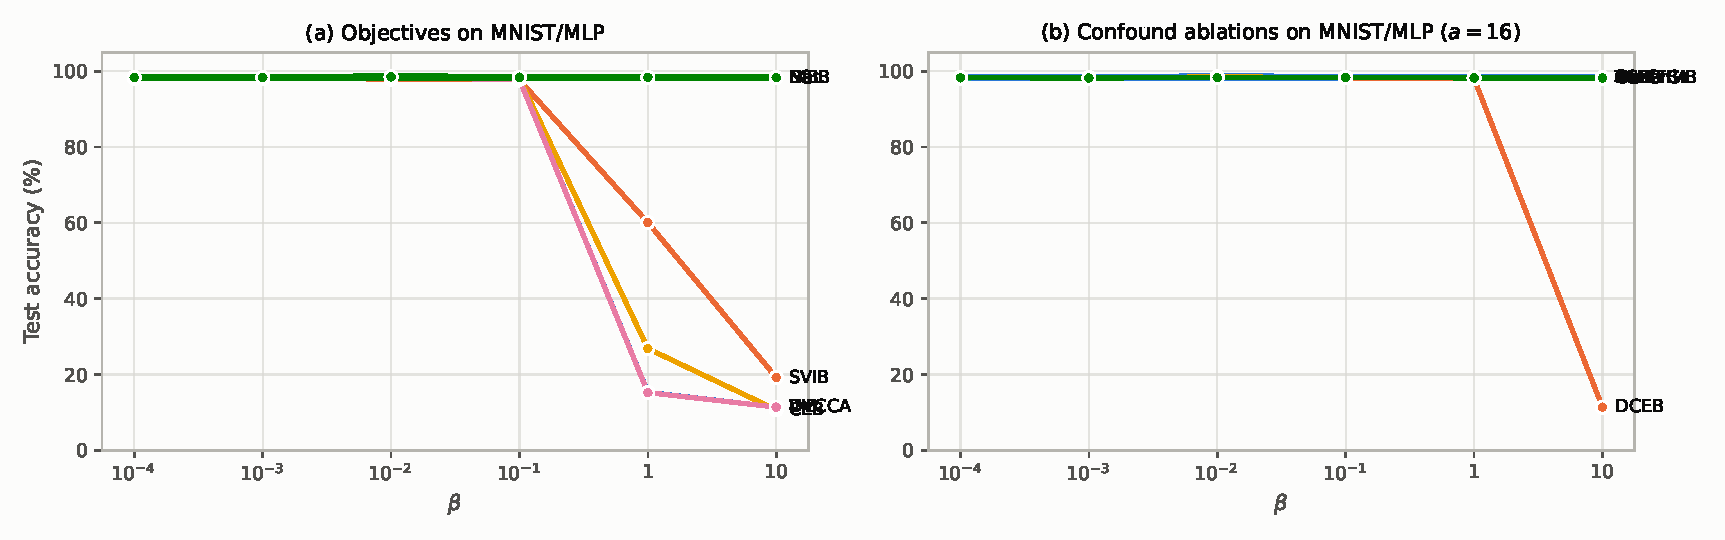
\includegraphics[width=\linewidth]{figures/beta_accuracy.pdf}
\caption{Test accuracy against $\beta$ (logarithmic axis) on MNIST/MLP. (a) The seven
objectives; (b) the confound ablations of Section~\ref{sec:ablation} at $a=16$. Lines
are means over 5 seeds; every series is labeled at its right end.}
\label{fig:betaacc}
\end{figure}

\begin{figure}[t]
\centering
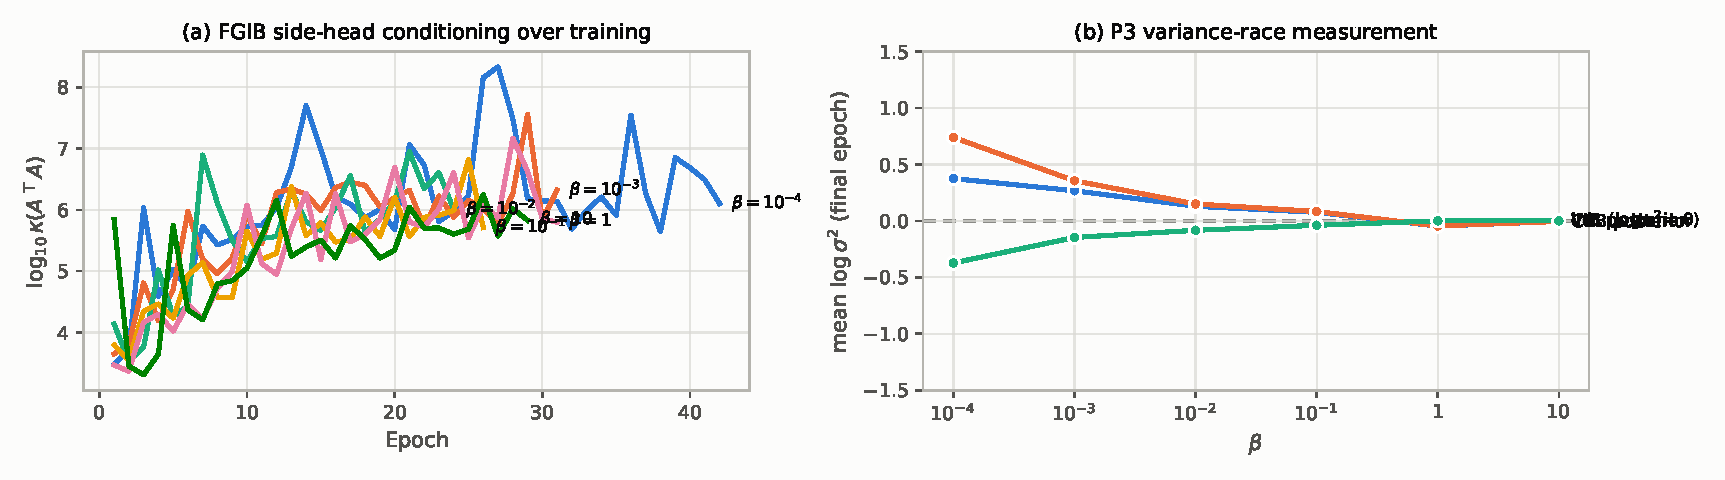
\includegraphics[width=\linewidth]{figures/diagnostics.pdf}
\caption{Diagnostics on MNIST/MLP. (a) $\log_{10}\kappa(A^{\top}A)$ of the FGIB side
head over training, one seed per $\beta$. (b) The P3 variance-race measurement: mean
log-variance at the final epoch against $\beta$ for CEB's posterior and prior and VIB's
posterior; the dashed line is the initialization $\log\sigma^2 = 0$.}
\label{fig:diag}
\end{figure}

\subsection{What we have not measured}
\label{sec:notyet}

Two of the three experiments this paper's own theory originally asked for are now in it
(Section~\ref{sec:ablation}): the variance-race measurement, and the
$\kappa(A^{\top}A)$ conditioning measurement over training. What remains open is on the
record here rather than in a reader's inference.
\emph{(i) Separating the
$\beta$-effect from the early-stopping effect.} Remark~\ref{rem:c-scale}(b) predicts that
the $\beta$-dependence of the equilibrium decays with training length; our runs use
patience 10, so training well past saturation and comparing converged KL across $\beta$
would test it. The cosine-classifier runs of Section~\ref{sec:ablation} enforce the
fixed-$c$ assumption of Proposition~\ref{prop:sweep} but do not remove early stopping.
\emph{(ii) Equal budget for the other methods.} The $a=16$ column of
Table~\ref{tab:main-std} gives FGIB the same 6-point budget as the comparison; the
converse --- giving VIB/CEB/DVCCA an extra temperature or variance hyperparameter
dimension --- is not run, so the comparison's rank ordering is only shown to survive
budget restriction for FGIB, not budget expansion for the others. \emph{(iii) The
remaining protocol asks.} All results come from one fixed $60/20/20$ split per dataset
(seed 42), so split-sensitivity is unmeasured; the AgeDB numbers use the image-level
split, under which $562$ of $567$ identities appear on both sides of the train/test
boundary (a subject-disjoint split is implemented in the released code and flagged in
Appendix~\ref{app:data}, but not run here). Beyond the theory's own asks, the robustness
properties that motivate
conditional bottlenecks in the first place --- adversarial robustness, OoD detection,
calibration, and resistance to memorizing random labels \citep{fischer2020ceb,
fischer2020cebrobust} --- are not evaluated here; the label-free anchor-distance score
$\min_y \KLd(q(z|x)\|\Ncal(a v_y, \tau^2 I))$ that FGIB's geometry makes available at
inference (Remark~\ref{rem:training-role}) is a hypothesis, not a result.

\section{Related work}

\paragraph{Variational bottlenecks.}
VIB \citep{alemi2017vib} bounds $I(X;Z)$ with a marginal prior; CEB
\citep{fischer2020ceb} bounds the residual $I(X;Z|Y)$ with a learned backward encoder and
is tighter by exactly $I(Y;Z)$ at the respective optima. FGIB inherits the
residual-level object and replaces the learned backward encoder with a frozen geometric
one; Proposition~\ref{prop:ordering} shows the resulting bound is looser in value by the
anchor gap, and Remark~\ref{rem:force} argues that this is what makes its force
persistent. DVCCA \citep{abdelaleem2025dvmib} sits in the same variational family with an
added reconstruction term, and inherits the marginal-prior corner (Table~\ref{tab:robust}
confirms this empirically).

\paragraph{Degeneracies of the IB Lagrangian.}
\citet{kolchinsky2019caveats} prove that in the deterministic scenario the IB curve is
piecewise linear, so the Lagrangian cannot sweep it, and repair this by squaring the
compression term. Our Proposition~\ref{prop:dead} shows CEB inherits the degeneracy over
its entire range, and Result~\ref{res:sweep} shows that a fixed reference supplies the
same strict convexity \emph{without} squaring --- while Table~\ref{tab:robust} shows that
squaring alone (SVIB) does not fix the collapse, since it leaves the corner where it was.
\citet{kolchinsky2019nib} avoid the parametric prior entirely with a non-parametric
pairwise bound; the two bounds are complementary, and our experiments locate the price of
that route in an inert knob.

\paragraph{Deterministic representations and infinite information.}
\citet{amjad2020learning} and \citet{kolchinsky2019nib} observe that $I(X;Z)$ is infinite
or ill-defined for deterministic continuous encoders, and \citet{saxe2018information}
question the empirical IB narrative on related grounds. Formal limits on measuring mutual
information from samples \citep{mcallester2020formal,tschannen2020mutual} apply to any
bound-as-meter reading, ours included. FGIB's response is architectural: keep the
inference path deterministic and confine the noise --- and thus the finite bound --- to a
side path that inference never reads.

\paragraph{Fixed geometric targets.}
Fixed geometric targets have a long history. Center loss pulls features toward learned
per-class centers \citep{wen2016center}; hyperspherical prototype networks place class
prototypes on a hypersphere a priori \citep{mettes2019hpn}; the final classifier itself
can be fixed with little accuracy loss \citep{hoffer2018fix}, in particular to the
vertices of a simplex equiangular tight frame \citep{zhu2021geometric,pernici2019regular};
and neural-collapse analyses show such configurations arise spontaneously in the
terminal phase of training \citep{papyan2020prevalence}. FGIB's compressed corner is a
neural-collapse-like geometry --- orthonormal class codes rather than the centered
simplex/ETF configuration of full neural collapse --- but the construction differs from
each of these in the role the geometry plays: it enters as the \emph{reference of a
variational bound}, i.e.\ as the design of the bottleneck's zero-penalty set, which is
what makes the compression term quadratic (Result~\ref{res:sweep}), the force persistent
(Result~\ref{res:endpoint}), and the regularizer carry a residual-information reading
for the auxiliary code (Result~\ref{res:equiv}) --- rather than as an auxiliary
classification loss. Table~\ref{tab:related} spells out the distinctions. We also report
the boundary of that claim honestly: on MNIST, replacing the KL by a plain center loss
with the same anchors reproduces FGIB's behavior (Section~\ref{sec:ablation}), so the
\emph{empirical} robustness is shared with fixed-prototype regularization, while the
bound reading and the sweep theory are specific to the variational form.

\begin{table}[t]
\centering
\small
\begin{tabular}{lccccc}
Method & Fixed geometry & Zero-penalty set & Variational bound & Regularizer on deployed repr. \\
\hline
VIB \citep{alemi2017vib} & --- & collapse (origin) & marginal KL on sampled $z$ & no (evaluates $\mu$) \\
CEB \citep{fischer2020ceb} & --- & underdetermined family & conditional KL on sampled $z$ & no (evaluates $\mu$) \\
center loss \citep{wen2016center} & learned centers & no bottleneck reading & --- & yes (same object) \\
HPN \citep{mettes2019hpn} & hypersphere (a priori) & --- & --- & yes (same object) \\
fixed classifier \citep{hoffer2018fix,zhu2021geometric,pernici2019regular} & simplex/ETF rows & --- & --- & yes (classifier, not regularizer) \\
FGIB (ours) & orthonormal anchors (a priori) & prescribed class codes & side-path conditional KL & side path only (bound read on $h$) \\
\end{tabular}
\caption{FGIB against the closest fixed-geometry and prototype regularizers. ``Zero-penalty
set'' is the set of representations where the regularizer vanishes. ``Variational bound''
asks whether the regularizer carries a KL/information interpretation. ``Regularizer on
deployed repr.'' asks whether the regularized object is the representation inference
consumes.}
\label{tab:related}
\end{table}

\section{Conclusion}

The high-regularization behavior of a variational bottleneck is decided by its
zero-penalty set, and the standard choices are poorly designed: the fixed marginal prior
of VIB places that set at collapse, the learned backward encoder of CEB leaves it
underdetermined so the optimizer --- not the objective --- selects the final label
geometry, and in both cases the bound certifies the noisy training code rather than the
deterministic representation inference deploys (a gradient-level variance race, in
contrast, fails to materialize in our measured runs). Designing the set directly --- an
orthonormal anchor frame fixed by construction, reached through a side head inference
never reads --- makes the compression term quadratic and hence the sweep well-posed at
fixed classifier scale, and turns the fully compressed corner into the prescribed
class-separated anchor configuration. Empirically, across 12 task$\times$backbone
settings and $5{,}100$ runs, that is worth a first-place mean rank under the
equal-budget configuration ($2.33$; $1.75$ over the full grid) and, more distinctively, a
compression knob that can be swept over a six-point grid spanning five orders of
magnitude without destroying the model on classification --- something no other objective
in the comparison manages. The ablations pin down what carries that robustness: on MNIST
it is the endpoint geometry, not the KL machinery, not the frozenness of the anchor
means, and not the deterministic path alone --- a plain center loss with the same
orthonormal anchors reproduces FGIB's curve. The KL's role is interpretive: an exact
variational upper bound on the residual information of the auxiliary noisy code, the
persistent force and convexified sweep of the theory; whether that interpretation tracks
the deployed representation beyond the aligned family remains open. The cross-dataset
reach of the geometry-only mechanism, in contrast, is now measured --- CentFGIB matches
FGIB at equal budget on all 12 settings (Section~\ref{sec:ablation}). The side
head is a second trainable party inside the KL, and we measured its cost:
$\kappa(A^{\top}A)$ becomes severely ill-conditioned ($10^{5.8}$--$10^{6.8}$ at the
final epoch, transient peaks to $10^{8.3}$), though predictive accuracy is unaffected on
MNIST --- so constraining $A$ by default, and the subject-disjoint and split-sensitivity
controls, are the natural next steps.

\subsection*{AI use statement}

(This section is \textbf{required} and does not count toward the page limit.)

In this work, we used generative AI tools (large-language-model assistants) for code
generation and refactoring, drafting and editing portions of the text, and checking
mathematical derivations. All AI-assisted work was reviewed and verified by the authors,
including every equation, table number and experimental claim. We take responsibility
for the final content of this work, including text, claims or artifacts produced with
the aid of generative AI. See the ICLR 2027 AI Policy for Authors for more details.

\subsection*{Ethics statement}

The datasets used are standard public benchmarks. One of them, AgeDB
\citep{moschoglou2017agedb}, consists of images of human faces annotated with age, and we
use it only as a scalar regression benchmark; we do not train or release face
recognition or demographic-inference models, and we make no claim that age estimates from
this data generalize fairly across populations. No new data was collected and no human
subjects were involved.

\subsection*{Reproducibility statement}

All results come from a single training entry point with a shared argument parser across
tasks, backbones and objectives; the exact grid is described in Section~\ref{sec:exp} and
every one of the $1{,}020$ configurations writes a log containing the per-run and averaged
test metrics. Tables~\ref{tab:main}--\ref{tab:main-std} are generated from those logs by a
single script (\texttt{make\_tables.py}) that re-derives the validation selection, so no
number in this paper is transcribed by hand; the paired statistics of
Table~\ref{tab:paired} (\texttt{make\_stats.py}) and the ablation table of
Table~\ref{tab:ablation} (\texttt{make\_ablation.py}) are generated the same way. All
proofs are in Appendix~\ref{app:theory}, with the assumptions of each
statement made explicit and the unproved items collected in a single scope remark. Data
preprocessing, splits (fixed seed 42) and caching are described in
Appendix~\ref{app:data}. Model selection uses validation scores only --- every tie-break
is a second validation quantity or fixed grid order --- and test scores are
read once per configuration.

\bibliographystyle{iclr2027_conference}
\begin{thebibliography}{99}

\bibitem[Abdelaleem et al.(2025)]{abdelaleem2025dvmib}
Eslam Abdelaleem, Ilya Nemenman, and K.~Michael Martini.
\newblock Deep variational multivariate information bottleneck --- a framework for
  variational losses.
\newblock \emph{Journal of Machine Learning Research}, 26:1--49, 2025.

\bibitem[Alemi et al.(2017)]{alemi2017vib}
Alexander~A. Alemi, Ian Fischer, Joshua~V. Dillon, and Kevin Murphy.
\newblock Deep variational information bottleneck.
\newblock In \emph{International Conference on Learning Representations}, 2017.

\bibitem[Amjad \& Geiger(2020)]{amjad2020learning}
Rana~Ali Amjad and Bernhard~C. Geiger.
\newblock Learning representations for neural network-based classification using the
  information bottleneck principle.
\newblock \emph{IEEE Transactions on Pattern Analysis and Machine Intelligence},
  42(9):2225--2239, 2020.

\bibitem[Cer et al.(2017)]{cer2017semeval}
Daniel Cer, Mona Diab, Eneko Agirre, I\~{n}igo Lopez-Gazpio, and Lucia Specia.
\newblock SemEval-2017 task 1: Semantic textual similarity multilingual and crosslingual
  focused evaluation.
\newblock In \emph{Proceedings of SemEval}, 2017.

\bibitem[Deng et al.(2009)]{deng2009imagenet}
Jia Deng, Wei Dong, Richard Socher, Li-Jia Li, Kai Li, and Li~Fei-Fei.
\newblock ImageNet: A large-scale hierarchical image database.
\newblock In \emph{IEEE Conference on Computer Vision and Pattern Recognition}, 2009.

\bibitem[Devlin et al.(2019)]{devlin2019bert}
Jacob Devlin, Ming-Wei Chang, Kenton Lee, and Kristina Toutanova.
\newblock BERT: Pre-training of deep bidirectional transformers for language
  understanding.
\newblock In \emph{NAACL-HLT}, 2019.

\bibitem[Dwivedi et al.(2023)]{dwivedi2023benchmarking}
Vijay~Prakash Dwivedi, Chaitanya~K. Joshi, Anh~Tuan Luu, Thomas Laurent, Yoshua Bengio,
  and Xavier Bresson.
\newblock Benchmarking graph neural networks.
\newblock \emph{Journal of Machine Learning Research}, 24(43):1--48, 2023.

\bibitem[Fischer(2020)]{fischer2020ceb}
Ian Fischer.
\newblock The conditional entropy bottleneck.
\newblock \emph{Entropy}, 22(9):999, 2020.

\bibitem[Fischer \& Alemi(2020)]{fischer2020cebrobust}
Ian Fischer and Alexander~A. Alemi.
\newblock CEB improves model robustness.
\newblock \emph{Entropy}, 22(10):1081, 2020.

\bibitem[He et al.(2016)]{he2016resnet}
Kaiming He, Xiangyu Zhang, Shaoqing Ren, and Jian Sun.
\newblock Deep residual learning for image recognition.
\newblock In \emph{IEEE Conference on Computer Vision and Pattern Recognition}, 2016.

\bibitem[Hochreiter \& Schmidhuber(1997)]{hochreiter1997lstm}
Sepp Hochreiter and J\"{u}rgen Schmidhuber.
\newblock Long short-term memory.
\newblock \emph{Neural Computation}, 9(8):1735--1780, 1997.

\bibitem[Hoffer et al.(2018)]{hoffer2018fix}
Elad Hoffer, Itay Hubara, and Daniel Soudry.
\newblock Fix your classifier: the marginal value of training the last weight layer.
\newblock In \emph{International Conference on Learning Representations}, 2018.

\bibitem[Kingma \& Ba(2015)]{kingma2015adam}
Diederik~P. Kingma and Jimmy Ba.
\newblock Adam: A method for stochastic optimization.
\newblock In \emph{International Conference on Learning Representations}, 2015.

\bibitem[Kipf \& Welling(2017)]{kipf2017gcn}
Thomas~N. Kipf and Max Welling.
\newblock Semi-supervised classification with graph convolutional networks.
\newblock In \emph{International Conference on Learning Representations}, 2017.

\bibitem[Kolchinsky et al.(2019a)]{kolchinsky2019caveats}
Artemy Kolchinsky, Brendan~D. Tracey, and Steven Van~Kuyk.
\newblock Caveats for information bottleneck in deterministic scenarios.
\newblock In \emph{International Conference on Learning Representations}, 2019a.

\bibitem[Kolchinsky et al.(2019b)]{kolchinsky2019nib}
Artemy Kolchinsky, Brendan~D. Tracey, and David~H. Wolpert.
\newblock Nonlinear information bottleneck.
\newblock \emph{Entropy}, 21(12):1181, 2019b.

\bibitem[LeCun et al.(1998)]{lecun1998mnist}
Yann LeCun, L\'{e}on Bottou, Yoshua Bengio, and Patrick Haffner.
\newblock Gradient-based learning applied to document recognition.
\newblock \emph{Proceedings of the IEEE}, 86(11):2278--2324, 1998.

\bibitem[Maas et al.(2011)]{maas2011imdb}
Andrew~L. Maas, Raymond~E. Daly, Peter~T. Pham, Dan Huang, Andrew~Y. Ng, and Christopher
  Potts.
\newblock Learning word vectors for sentiment analysis.
\newblock In \emph{Annual Meeting of the Association for Computational Linguistics}, 2011.

\bibitem[McAllester \& Stratos(2020)]{mcallester2020formal}
David McAllester and Karl Stratos.
\newblock Formal limitations on the measurement of mutual information.
\newblock In \emph{International Conference on Artificial Intelligence and Statistics},
  2020.

\bibitem[Mettes et al.(2019)]{mettes2019hpn}
Pascal Mettes, Elise van der Pol, and Cees~G.~M. Snoek.
\newblock Hyperspherical prototype networks.
\newblock In \emph{Advances in Neural Information Processing Systems}, 2019.

\bibitem[Moschoglou et al.(2017)]{moschoglou2017agedb}
Stylianos Moschoglou, Athanasios Papaioannou, Christos Sagonas, Jiankang Deng, Irene
  Kotsia, and Stefanos Zafeiriou.
\newblock AgeDB: The first manually collected, in-the-wild age database.
\newblock In \emph{CVPR Workshops}, 2017.

\bibitem[Pace \& Barry(1997)]{pace1997sparse}
R.~Kelley Pace and Ronald Barry.
\newblock Sparse spatial autoregressions.
\newblock \emph{Statistics \& Probability Letters}, 33(3):291--297, 1997.

\bibitem[Papyan et al.(2020)]{papyan2020prevalence}
Vardan Papyan, X.~Y. Han, and David~L. Donoho.
\newblock Prevalence of neural collapse during the terminal phase of deep learning
  training.
\newblock \emph{Proceedings of the National Academy of Sciences}, 117(40):24652--24663,
  2020.

\bibitem[Pennington et al.(2014)]{pennington2014glove}
Jeffrey Pennington, Richard Socher, and Christopher~D. Manning.
\newblock GloVe: Global vectors for word representation.
\newblock In \emph{Conference on Empirical Methods in Natural Language Processing}, 2014.

\bibitem[Pernici et al.(2019)]{pernici2019regular}
Federico Pernici, Matteo Bruni, Claudio Baecchi, and Alberto~Del Bimbo.
\newblock Fix your features: stationary and maximally discriminative embeddings using
  regular polytope (fixed classifier) networks.
\newblock \emph{arXiv preprint arXiv:1902.10441}, 2019.

\bibitem[Rahimi \& Recht(2008)]{rahimi2008random}
Ali Rahimi and Benjamin Recht.
\newblock Random features for large-scale kernel machines.
\newblock In \emph{Advances in Neural Information Processing Systems}, 2008.

\bibitem[Saxe et al.(2018)]{saxe2018information}
Andrew~M. Saxe, Yamini Bansal, Joel Dapello, Madhu Advani, Artemy Kolchinsky, Brendan~D.
  Tracey, and David~D. Cox.
\newblock On the information bottleneck theory of deep learning.
\newblock In \emph{International Conference on Learning Representations}, 2018.

\bibitem[Sen et al.(2008)]{sen2008collective}
Prithviraj Sen, Galileo Namata, Mustafa Bilgic, Lise Getoor, Brian Galligher, and Tina
  Eliassi-Rad.
\newblock Collective classification in network data.
\newblock \emph{AI Magazine}, 29(3):93--106, 2008.

\bibitem[Tishby et al.(1999)]{tishby1999ib}
Naftali Tishby, Fernando~C. Pereira, and William Bialek.
\newblock The information bottleneck method.
\newblock In \emph{Allerton Conference on Communication, Control and Computing}, 1999.

\bibitem[Tschannen et al.(2020)]{tschannen2020mutual}
Michael Tschannen, Josip Djolonga, Paul~K. Rubenstein, Sylvain Gelly, and Mario Lucic.
\newblock On mutual information maximization for representation learning.
\newblock In \emph{International Conference on Learning Representations}, 2020.

\bibitem[Wang et al.(2019)]{wang2019glue}
Alex Wang, Amanpreet Singh, Julian Michael, Felix Hill, Omer Levy, and Samuel~R. Bowman.
\newblock GLUE: A multi-task benchmark and analysis platform for natural language
  understanding.
\newblock In \emph{International Conference on Learning Representations}, 2019.

\bibitem[Wen et al.(2016)]{wen2016center}
Yandong Wen, Kaipeng Zhang, Zhifeng Li, and Yu Qiao.
\newblock A discriminative feature learning approach for deep face recognition.
\newblock In \emph{European Conference on Computer Vision}, pages 499--515, 2016.

\bibitem[Zhang et al.(2015)]{zhang2015character}
Xiang Zhang, Junbo Zhao, and Yann LeCun.
\newblock Character-level convolutional networks for text classification.
\newblock In \emph{Advances in Neural Information Processing Systems}, 2015.

\bibitem[Zhu et al.(2021)]{zhu2021geometric}
Zhihui Zhu, Tianyu Ding, Jinxin Zhou, Xiao Li, Chong You, Jeremias Sulam, and Qing Qu.
\newblock A geometric analysis of neural collapse with unconstrained features.
\newblock In \emph{Advances in Neural Information Processing Systems}, 2021.

\end{thebibliography}

\appendix

\section{Complete theory: proofs of the failure channels and of the FGIB mechanism}
\label{app:theory}

The remainder of this appendix is the full development: Part~I proves the four failure
channels of Section~\ref{sec:prelim}, Part~II proves the FGIB results of
Section~\ref{sec:method}, and its final subsection (Section~\ref{sec:limits}) is a
complete ledger separating what is proved from what is open or conditional.

% fgib_theory.tex —— FGIB 完整理论推导（四个问题的证明 + FGIB 机制的证明）
% 本文件合并自 fgib_ceb_collapse.tex / fgib_degeneration.tex / fgib_bound.tex / fgib_linear.tex，
% 原四文件可删除；全部标签名保持不变，fgib_intro.tex / fgib_method.tex 的 \ref 不受影响。
% 用法：\usepackage{amsmath,amssymb,amsthm}，正文处 % fgib_theory.tex —— FGIB 完整理论推导（四个问题的证明 + FGIB 机制的证明）
% 本文件合并自 fgib_ceb_collapse.tex / fgib_degeneration.tex / fgib_bound.tex / fgib_linear.tex，
% 原四文件可删除；全部标签名保持不变，fgib_intro.tex / fgib_method.tex 的 \ref 不受影响。
% 用法：\usepackage{amsmath,amssymb,amsthm}，正文处 % fgib_theory.tex —— FGIB 完整理论推导（四个问题的证明 + FGIB 机制的证明）
% 本文件合并自 fgib_ceb_collapse.tex / fgib_degeneration.tex / fgib_bound.tex / fgib_linear.tex，
% 原四文件可删除；全部标签名保持不变，fgib_intro.tex / fgib_method.tex 的 \ref 不受影响。
% 用法：\usepackage{amsmath,amssymb,amsthm}，正文处 \input{fgib_theory.tex}。
% 记号沿用 Fischer (2020)、Kolchinsky & Tracey (2019, Caveats)、Kolchinsky et al. (2017, NIB)、
% Alemi et al. (2017, VIB)。
%
% 核心结论（FGIB 论文问题陈述与解法）：
% 第一部分（四条失效通道）：
%   P1 退化继承（死旋钮）：CEB ≡ IB(β=1+γ>1)，确定性场景下所有 γ>0 的唯一最优解钉在角点，
%      γ 扫不出任何中间点（SIB Caveat 1 的退化半区，经 β'=1/(1+γ)∈(0,1) 映射）。
%      该角点恰是 CEB 自己的 MNI 目标，rem:mni 正面处理这一反驳；
%   P2 证书盲视 + 1:β 交换率：T_α 流形上 ReX 恒为 0（证书对标签保留量完全盲视），
%      且目标以 1 nat 标签信息 ↔ β nat 认证残差的比率交换；
%   P3 方差竞赛：KL 两侧皆可训练，分类项压 σ→0、钳位处退化为权重 e^{10} 的均值匹配。
%      (ii)(iii) 是受力方向分析而非收敛证明，且可实测（rem:p3-status）；
%   P4 对象错位：两种方法的界都只界住各自的含噪码，都不界住确定性连续推理表示的残差
%      （后者为 +∞）。差别是结构性的（噪声在不在推理路径上），不是紧度排序。
% 第二部分（FGIB 机制，以及它没能关闭的通道）：
%   M1 等价性：旁路 = 固定 A 下作用在 h+已知噪声上的 CEB 瓶颈（逐步成立，非全程固定参考）；
%   M2 扫参：固定分类器尺度 c 时 L_β(s)=CE(s)+(β/2)(s−a)² 严格凸、每 β 唯一内点、曲线严格凹；
%      c 自由时下确界对所有 β 均为 0（rem:c-scale，给出权重归一化分类器的架构修法）；
%   M3 证书：gap 恒等式 + 矩匹配 + 固定编码器下的值排序；固定参考的力持续性成立，
%      但侧头 A 是推理无关的第二个自由方（rem:A-channel），构成未关闭的通道。
%
% 修订记录（第二轮）：理论/实现分层后统一引入锚点方差 τ²（先验 N(a v_y, τ²I)，默认 τ²=1，
% 后验方差最优 σ²*=τ²，σ_p 为公共方差记号；point-anchor 极限统一写为 τ→0）；理论旁路固定为
% 可逆线性头 T(h)=Ah（实现用带 bias 的 nn.Linear 近似，见理论-代码分层 caveat）；
% 明确 sweep 证明的是对齐族上 KL–CE surrogate 曲线（rem:surrogate），不是 IB 互信息曲线；
% 无穷互信息结论统一挂靠分布性 standing assumption；rem:c-scale 的架构修法收紧为
% 固定温度 cosine 分类器（weight decay 只缓解不发散）；a=0 退化点、条件数表述、
% 梯度消失条件、row-space 表述等小项修正。
%
% 修订记录（第一轮）：删除三处错误论断——(1) P3 原称 ReX≈0 时 I(X;Z|Y) 发散，与 gap 恒等式矛盾；
% (2) prop:object(c) 原称 FGIB 的界"更紧/唯一有效"，由 DPI 不成立；(3) prop:conditioning(iii)
% 原从 Gram 恒等式推出条件数为 1，有反例。修正 P2 的换算、Caveat 2 的主张、rem:frame 的
% A^T/V^T、mu_head 的仿射与非推理路径身份。未证结论统一收入 sec:limits。

\newtheorem{lemma}{Lemma}
\newtheorem{proposition}{Proposition}
\newtheorem{remark}{Remark}

% =====================================================================
\section*{Part I. The four failure channels of the conditional bottleneck}
% =====================================================================

\textbf{Notation.}
$X$ is the input and $Y$ the label with $K$ classes; the encoder induces the Markov chain
$Y - X - Z$. The \emph{deterministic scenario} is $Y = f(X)$ ($H(Y|X) = 0$). Following
Fischer (2020), we write the MNI point $I(X;Y) = I(X;Z) = I(Y;Z)$ (Eq.~1), the
chain-rule identity $I(X;Z|Y) = I(X;Z) - I(Y;Z)$ (Eq.~4), the CEB objective
$\mathrm{CEB} \equiv \min_Z I(X;Z|Y) - \gamma I(Y;Z)$ (Eq.~5), the IB objective
$\mathrm{IB} \equiv \min_Z I(X;Z) - \beta_{\mathrm{IB}} I(Y;Z)$ (Eq.~16), the
variational objective
$\mathrm{VCEB} \equiv \min_{e,b,c} \langle \log e(z|x)\rangle - \langle \log b(z|y)\rangle
- \gamma \langle \log c(y|z)\rangle$ (Eq.~15), and the residual certificate
$\mathrm{ReX} \equiv \langle \log e(z|x)\rangle - \langle \log b(z|y)\rangle
\ge I(X;Z|Y)$ (Eq.~20), where $b(z|y)$ is a \emph{trainable} backward encoder (we write
$q(z|x)$ for Fischer's encoder $e(z|x)$; the two notations are interchangeable
throughout). In the loss convention $\mathrm{CE} + \beta\,\mathrm{KL}$ used throughout, the weights are
$\beta = 1/\gamma$ and $\beta_{\mathrm{IB}} = 1 + \gamma = 1 + 1/\beta$. Following
Kolchinsky \& Tracey (2019), we write the IB curve $F(r)$ (their Eq.~1), the IB
Lagrangian $L^{\mathrm{IB}}_\beta = I(Y;T) - \beta I(X;T)$ (their Eq.~2), the
DPI-saturating manifold $T_\alpha := B_\alpha \cdot Y$ (their Eq.~6), the bound
$L^{\mathrm{IB}}_\beta \le (1-\beta)H(Y)$ (their Eq.~7), and their footnote~4 (the
$\beta > 1$ regime of trivial maximizers). The variational objects are
\begin{align*}
R &= \mathbb{E}\big[\operatorname{KL}(q(z|x)\,\|\,m(z))\big] \ge I(X;Z)
&&\text{(VIB rate, marginal prior $m$; Fischer Eq.~19, Alemi et al.\ Eq.~14)} \\
\mathrm{ReX} &= \mathbb{E}\big[\operatorname{KL}(q(z|x)\,\|\,b_\theta(z|y))\big]
\ge I(X;Z|Y)
&&\text{(CEB residual; Fischer Eq.~20)} \\
\widehat I &= -\frac{1}{N}\sum_i \ln\Big[\frac{1}{N}\sum_j
e^{-\|f_i-f_j\|^2/(2\sigma^2)}\Big] \ge I(X;M)
&&\text{(NIB, non-parametric; Eq.~16, the homoscedastic case of Eq.~10)} \\
\mathrm{ReX}_F &= \mathbb{E}\big[\operatorname{KL}(q(z|x)\,\|\,r(z|y))\big]
\ge I(X;Z|Y)
&&\text{(FGIB, fixed anchor)}
\end{align*}
(Fischer 2020, Eqs.~18--20; Alemi et al.\ 2017, Eq.~14; Kolchinsky et al.\ 2017,
Eqs.~10 and 16). Fischer's comparison of the first two: at the respective prior optima
($m = q(z)$, $b = q(z|y)$), $\mathrm{ReX} = R - I(Y;Z)$ --- the conditional prior removes
exactly the retained label information, so CEB's bound is tighter than VIB's by
$I(Y;Z)$. We ask the same question one level down: where does FGIB's fixed-anchor bound
sit relative to CEB's learnable-backward bound?

\begin{proposition}[Channel P1, dead knob: every $\gamma > 0$ selects the same corner]\label{prop:dead}
Assume $Y = f(X)$. For every $\gamma > 0$,
\begin{equation}
\min_Z L_\gamma(Z) = -\gamma H(Y),
\qquad
L_\gamma(Z) := I(X;Z|Y) - \gamma I(Y;Z),
\label{eq:min}
\end{equation}
attained exactly on the corner family
$\{Z : I(Y;Z) = H(Y),\; I(X;Z|Y) = 0\}$ (e.g.\ $Z = Y$, or $Z = (Y, N)$ with
$N \perp X \mid Y$): the corner is unique in the information plane, while at the
representation level it is an entire family. Consequently the map
$\gamma \mapsto \big(I(X;Z^*|Y),\, I(Y;Z^*)\big)$ is constant: no interior point of the
IB curve is ever a Lagrangian minimizer, and CEB inherits the deterministic degeneration
of the Caveats paper (their Issue~1) over its \emph{entire} parameter range, since
$\beta_{\mathrm{IB}} = 1 + \gamma > 1$ always.
\end{proposition}

\begin{proof}
By Fischer's Eq.~4, $L_\gamma(Z) = I(X;Z) - (1+\gamma)I(Y;Z)$. The DPI
($I(Y;Z) \le I(X;Z)$, by the Markov chain $Y - X - Z$) gives
\begin{equation}
L_\gamma(Z) \ge I(Y;Z) - (1+\gamma)\,I(Y;Z)
= -\gamma\,I(Y;Z) \ge -\gamma H(Y),
\label{eq:chain}
\end{equation}
with equality iff both inequalities bind: $I(X;Z) = I(Y;Z)$ and $I(Y;Z) = H(Y)$.
$Z = Y$ attains the bound. Fischer (2020, p.~7) states the underlying equivalence
explicitly: CEB and IB are the same objective for $\gamma = \beta_{\mathrm{IB}} - 1$.
In the Caveats paper's maximizing convention, minimizing $L_\gamma$ is maximizing
$L^{\mathrm{IB}}$ with $\beta' = 1/\beta_{\mathrm{IB}} = 1/(1+\gamma) \in (0,1)$ ---
precisely the range in which their Eq.~7 pins every maximizer at the copy corner (their
Issue~1); their footnote~4 covers the complementary regime $\beta' > 1$ (i.e.\
$\gamma < 0$, outside CEB's range), whose maximizers are the trivial collapse. \hfill\qed
\end{proof}

\begin{remark}[The corner is the MNI point: why that does not rescue the knob]\label{rem:mni}
In the deterministic scenario the corner of Proposition~\ref{prop:dead} \emph{is} the MNI
point: $I(Y;Z) = H(Y) = I(X;Y)$ together with $I(X;Z|Y) = 0$ gives
$I(X;Y) = I(X;Z) = I(Y;Z)$, which is Fischer's Eq.~1. CEB's declared target and the
degenerate attractor therefore coincide, and Kolchinsky \& Tracey concede the point
themselves (their Section~4): ``if $Y = f(X)$ and one's goal is precisely to find the corner
point $\langle H(Y), H(Y)\rangle$ (maximum compression at no prediction loss), then our
results suggest that the IB Lagrangian provides a robust way to do so, being invariant to
the particular choice of $\beta$.'' Read that way, Proposition~\ref{prop:dead} states
hyperparameter robustness rather than failure. Three things keep it from closing the matter.
\begin{enumerate}
\item[(i)] \emph{The corner is one point in the information plane and an entire equivalence
class of representations.} The objective is exactly constant on
$\{Z : I(Y;Z) = H(Y),\ I(X;Z|Y) = 0\}$, which contains $Z = Y$, $Z = (Y,N)$ with
$N \perp X \mid Y$, and every bijective recoding of these. Adversarial robustness, OoD
detection and calibration --- the properties CEB is argued for --- are properties of the
\emph{geometry} of $Z$, on which the objective has no opinion; which member of the class is
reached is settled by the optimizer. That is channels P3 and P4 below.
\item[(ii)] \emph{CEB's own reading of the knob is unavailable at the exact optimum.}
Fischer (2020, p.~7) writes ``$\rho < 0$ may capture less than the MNI. $\rho > 0$ may
capture more'', whereas Proposition~\ref{prop:dead} places every $\gamma > 0$ at the MNI
point exactly. His argument for preferring $\gamma = 1$ is correspondingly not about
minimizers but about the optimizer: weighting the two appearances of $I(Y;Z)$ differently
``forces the optimization procedure to count bits of $I(Y;Z)$ in two different ways'' (his
Eq.~8 and surrounding discussion).
\item[(iii)] \emph{The knob does move trained models, which locates what it acts on.} On
Fashion MNIST --- a deterministically labelled dataset --- Fischer's own Figure~4 reports
the rate lower bound $R_X$ rising from $\approx 2.0$ to $\approx 5.0$ nats as $\rho$ goes
from $-1$ to $5$, with $\rho = 0$ landing on $I(X;Y) = \log 10 \approx 2.3$ nats. Since
every $\gamma > 0$ shares one exact optimum, that axis is not a path along the IB curve: it
is the distance between the optimum of the variational objective over a restricted family
and the point at which training was stopped. A knob acting through the approximation error
is precisely the knob that Propositions~\ref{prop:flat} and~\ref{prop:variance} show cannot
be read off the certificate.
\end{enumerate}
Kolchinsky \& Tracey state that their results ``are based on analytically-provable
properties of the IB curve, i.e., global optima'' and ``do not concern practical issues of
optimization''; Proposition~\ref{prop:flat} supplies the finite-$\beta$ variational
counterpart. The account is owed by any method reporting a $\beta$-sweep on
deterministically labelled data --- FGIB and the experiments of this paper included
(Remark~\ref{rem:c-scale}).
\end{remark}

\begin{proposition}[Channel P2, a blind certificate and a $1{:}\beta$ exchange rate]\label{prop:flat}
On the manifold $T_\alpha = B_\alpha \cdot Y$ of the Caveats paper (their Eq.~6),
$I(X;T_\alpha|Y) = 0$ for every $\alpha$, and with the optimal backward encoder and
classifier,
\begin{equation}
\mathrm{ReX}(T_\alpha) = 0,
\qquad
\mathrm{CE}(T_\alpha) = H(Y) - I(Y;T_\alpha) =: \delta_\alpha,
\qquad
\mathrm{VCEB}(T_\alpha) = \gamma\,\delta_\alpha .
\label{eq:vceb}
\end{equation}
Two consequences.
\emph{(a) The certificate is blind to label retention.} $\mathrm{ReX} = 0$ holds from the
total collapse ($\alpha = 0$, no label information) to the full copy ($\alpha = 1$), so its
tightness is compatible with retaining all, part, or none of $Y$. Fischer's reading of the
certificate as a meter --- ``observing ReX tells us exactly how many bits we are from the
MNI point'' (p.~7) --- therefore holds only along the $I(X;Z|Y)$ axis; on the necessity axis
the meter reads $0$ at chance level.
\emph{(b) Exchange rate.} With the optimal classifier the objective is
$L = \mathrm{CE} + \beta\,\mathrm{ReX} = \delta + \beta\,\mathrm{ReX}$, so it is indifferent
between giving up $\delta$ nats of label information and saving $\delta/\beta$ nats of
certified residual. In the heavy-regularization regime the bottleneck is supposed to act in,
the whole label axis --- up to $H(Y)$ nats --- is purchasable for $H(Y)/\beta$ nats of
certified compression.
\end{proposition}

\begin{proof}
$T_\alpha$ is a function of $Y$ alone, so $T_\alpha \perp X \mid Y$ and
$I(X;T_\alpha|Y) = 0$; the Caveats paper shows $I(Y;T_\alpha)$ sweeps $[0, H(Y)]$.
With the true backward encoder ($b = p(z|y)$) the certificate is tight:
$\mathrm{ReX} = I(X;T_\alpha|Y) = 0$ (Fischer Eqs.~9--11, 20). The optimal classifier
achieves $\langle \log c(y|z)\rangle = -H(Y|T_\alpha)$ (Fischer Eq.~12), i.e.\
$\mathrm{CE} = H(Y|T_\alpha) = \delta_\alpha$, and the VCEB value follows from Eq.~15.
Part~(b) is the definition of the objective evaluated at $\mathrm{CE} = \delta$.
\hfill\qed
\end{proof}

\begin{remark}[What the flatness claim is, and what it is not]\label{rem:convention}
An earlier form of this argument read the near-optimality band off the \emph{value}
$\mathrm{VCEB} = \gamma\delta \to 0$. That reading is a scaling artifact:
$\mathrm{VCEB} = \gamma\,(\mathrm{CE} + \beta\,\mathrm{ReX}) = \gamma L$, so the two
conventions differ by a positive factor and share their minimizers, and on $T_\alpha$ itself
the objective is $L = \delta$ in either convention and strictly prefers $\alpha = 1$. What
is convention-free is the \emph{ratio} of Proposition~\ref{prop:flat}(b): the prediction
term is weaker than the compression term by exactly the factor $\beta$, so in units of the
compression term the entire manifold lies within $H(Y)/\beta$ of optimal. Under a
scale-invariant optimizer (Adam, used throughout the experiments) only the ratio matters;
under plain SGD at fixed learning rate the convention additionally rescales the effective
step size. Combined with Proposition~\ref{prop:flat}(a) --- no certified compression is
bought anywhere on the manifold --- the operative statement is that the label axis is cheap
and unmetered, not that the objective is literally flat along it.
Pushing $\beta$ up also drives $\beta_{\mathrm{IB}} = 1 + 1/\beta \to 1^{+}$: the objective
approaches the Caveats paper's $\beta = 1$ degeneracy (their Eq.~7 discussion), at which
\emph{every} point of the diagonal is simultaneously optimal, from above. Fischer (2020,
p.~7) anticipates the direction --- ``$\rho < 0$ may capture less than the MNI'' --- but by
Proposition~\ref{prop:dead} that cannot happen at the exact optimum;
Proposition~\ref{prop:flat} gives the rate at which the variational objective is willing to
let it happen.
\end{remark}

\begin{remark}[Approximately deterministic labels]\label{rem:approx}
The Caveats paper (Appendix~C, Issue~1) shows that when $Y$ is only $\epsilon$-close to
deterministic, all optimizers fall within $O(-\epsilon\log\epsilon)$ of a single corner:
the dead-knob statement of Proposition~\ref{prop:dead} degrades gracefully, and the
near-optimality band of Proposition~\ref{prop:flat} is perturbed by the same order.
\end{remark}

\begin{proposition}[Channel P3, collusion collapse: the variance race and the overfit channel]\label{prop:variance}
For the diagonal Gaussian family $e(z|x) = \mathcal{N}(m(x), \sigma^2 I)$,
$b(z|y) = \mathcal{N}(g(y), \tau^2 I)$ (the implementation's setup, with the
\texttt{logvar} clamp $[-10, 10]$ of \texttt{kl\_divergence}), and a \emph{linear}
classifier $c(z) = Wz + b$ (the implementation's classifier is \texttt{nn.Linear}):
\begin{enumerate}
\item[(i)] for fixed means, $\operatorname{KL}$ is minimized over $\sigma^2$ at
$\sigma^2 = \tau^2$, with value $\tfrac{1}{2\tau^2}\|m - g\|^2$ --- a pure mean-matching
term;
\item[(ii)] the classifier term favors $\sigma^2 \to 0$:
$\mathrm{CE}(c(z), y) = -\log \mathrm{softmax}_y(Wz+b)$ is convex in $z$ (log-sum-exp
of an affine function of $z$, minus a linear term --- the convexity claim requires $c$
affine), so Jensen gives
$\mathbb{E}_z[\mathrm{CE}(c(z), y)] \ge \mathrm{CE}(c(m), y)$. The KL's derivative in
$\sigma^2$ vanishes at $\sigma^2 = \tau^2$, but along the matched line it \emph{resists}
shrinking $\tau^2$ while the means are unmatched
($\partial \operatorname{KL}/\partial \tau^2|_{\sigma^2=\tau^2}
= -\|m-g\|^2/(2\tau^4) < 0$). The joint dynamics therefore runs in two stages: the mean
matching $m \to g$ completes first (with weight $1/\tau^2$, which grows as $\tau$
shrinks), and once $\|m-g\| \to 0$ the variance race is unopposed --- the classifier
drives $\sigma^2 \to 0$ with $\tau^2$ following the moment-matched value --- until the
clamp at $s = e^{-10}$, where the encoder collapses toward the deterministic code
$z \approx g(y)$ and
$\mathrm{ReX} = \tfrac{1}{2s}\mathbb{E}\|m(x) - g(y)\|^2$: a mean-matching force of
weight $1/s = e^{10} \approx 2.2\times10^{4}$ between two \emph{trainable} maps;
\item[(iii)] the certified object and the deployed object separate. By the gap lemma
(Lemma~\ref{lem:gap}) $\mathrm{ReX} = I(X;Z|Y) + \Delta \ge I(X;Z|Y)$, so a small
$\mathrm{ReX}$ \emph{entails} a small residual for the stochastic training code --- the
certificate cannot under-report its own object. What it does not control is the relation
between the training code and the deployed representation. Exact mean matching
($m(x) = g(y)$) makes both objects class-constant, so both residuals vanish; the
scenario of interest is the \emph{near}-match regime, where
$\mathbb{E}\,\|m(X) - g(Y)\|^2 = o(s)$ keeps $\mathrm{ReX}$ small while the deployed
continuous $m$ retains within-class variation, and any non-class-constant continuous
$m$ has $I(X;m(X)|Y) = +\infty$ under the standing non-atomic assumption (the
pathology of deterministic networks, Amjad \&
Geiger 2018; Kolchinsky et al.\ 2017). The variance race therefore moves the
\emph{certified} object toward a noise-dominated class-constant code while the
\emph{deployed} object can keep diverging residual --- and the encoder is fitted to the
backward encoder's per-class targets, memorizing the label code $g(y)$ rather than
being told what residual to erase, while the certificate reports $\mathrm{ReX} \approx
0$ on a code that inference does not use.
\end{enumerate}
\end{proposition}

\begin{proof}
The closed form
$\operatorname{KL} = \tfrac{d}{2}\big[\sigma^2/\tau^2 + \|m-g\|^2/(d\tau^2)
- 1 + \ln(\tau^2/\sigma^2)\big]$ has derivative $\tfrac{d}{2}(1/\tau^2 - 1/\sigma^2)$
in $\sigma^2$, so the variance optimum is $\sigma^2 = \tau^2$, giving (i); at
$\sigma^2 = \tau^2 = s$ the value is $\|m-g\|^2/(2s)$. For (ii): $\mathrm{CE}(c(z), y)$ has Hessian
$\operatorname{diag}(p) - pp^{\top} \succeq 0$ (the categorical Fisher information), so
it is convex in $z$ and Jensen gives the stated inequality; the same Hessian identity makes
$\sigma^2 \mapsto \mathbb{E}_z[\mathrm{CE}(c(z),y)]$ non-decreasing (Gaussians of larger
variance dominate in convex order), strictly increasing in $\sigma^2$ wherever the
classifier is unsaturated, so that term pushes $\sigma^2$ down. The KL's partial derivatives at the
matched point are $\partial_{\sigma^2}\operatorname{KL} = 0$ and
$\partial_{\tau^2}\operatorname{KL} = -\|m-g\|^2/(2\tau^4) < 0$, so the KL pulls
$\tau^2$ up until the means match, while the mean-matching gradient on the encoder is
$(m - g)/\tau^2$; once $\|m-g\| \to 0$ the race to the clamp is unopposed. For (iii): the
gap identity (Lemma~\ref{lem:gap}) forces the certified residual and the certificate to
vanish together; the divergence attaches to the deployed mean $m(x)$ whenever it is not
class-constant (Amjad \& Geiger; Kolchinsky et al.). \hfill\qed
\end{proof}

\begin{remark}[Status of the two-stage account]\label{rem:p3-status}
Parts~(ii) and~(iii) are a stationarity-and-direction-of-force argument, not a convergence
proof: the ``two stages'' presume a time-scale separation (mean matching completes before
the variance race) that is not established here. The account is directly falsifiable in
this codebase: log the mean posterior log-variance and the fraction of units at the clamp
$s = e^{-10}$ during CEB training. \emph{We ran the test.} On MNIST, across all six
$\beta$ settings and 5 seeds (Section~\ref{sec:ablation} of the main paper), the trained
posterior and prior log-variances of CEB remain near their initialization ($\sigma^2 =
\tau^2 = 1$, mean $\log\sigma^2$ within $0.74$ of zero, clamp fraction $0.0$ at every
epoch of every run). At the early-stopping time scale of the experimental protocol, the
variance race therefore does not materialize, and
Proposition~\ref{prop:variance}(iii) is empirically void for those runs: Part~(iii)
stands as a sharp hypothesis about what longer training or different schedules would
produce, the force analysis of (i)--(ii) as the only proved content, and the
measurement itself as the finding.
\end{remark}

\begin{remark}[Train--evaluation mismatch]\label{rem:mismatch}
The classifier is trained on the sampled code $z$ and evaluated on the mean $m(x)$
(Fischer 2020, Appendix~A.1). Proposition~\ref{prop:variance}(ii) is the force that
closes this gap by destroying the noise altogether ($\sigma \to 0$), at which point the
bottleneck's stochasticity --- the object the bound is defined on --- disappears.
\end{remark}

\begin{proposition}[Channel P4, certificate-object mismatch: neither bound is an upper bound on the deployed representation]\label{prop:object}
(a)~\emph{CEB}. The classifier consumes the sampled code $Z$ at training and the mean
$\mu(X)$ at evaluation (Fischer 2020, Appendix~A.1). At the variance-optimal posterior,
$\sigma(x) \equiv \sqrt{S_\theta(y)}$ (the backward encoder's per-class standard
deviation) is class-constant, so $Z = \mu(X) + \sqrt{S_\theta(Y)}\,\varepsilon$ is a
noisy function of $\mu(X)$ given $Y$; by the DPI,
\begin{equation}
I(X; Z | Y) \;\le\; I(X;\, \mu(X) | Y) ,
\label{eq:dpi}
\end{equation}
strictly so whenever the noise destroys within-class detail. Hence CEB's certificate
$\mathrm{ReX} \ge I(X;Z|Y)$ is a bound on the \emph{training code}, not on the residual
of the representation deployed at inference. The gap is not a small correction: whenever
$\mu$ is a continuous map that is not class-constant, $I(X;\mu(X)|Y) = +\infty$ under
the standing non-atomic assumption (Amjad \& Geiger 2020; Kolchinsky et al.\ 2017), so
no finite quantity --- CEB's certificate included --- bounds the deployed residual from
above. The CE term presses the noise
toward $0$ (by Jensen, $\mathbb{E}_z[\mathrm{CE}(c(z),y)] \ge \mathrm{CE}(c(\mu),y)$),
but no finite $\sigma$ closes the gap.
(b)~\emph{FGIB}. The inference path is $h$ at both training and evaluation; the side
noise of Proposition~\ref{prop:inverse} is not part of any inference path. By the DPI
applied to the same perturbed-variable construction,
\begin{equation}
I(X;\, h + \tau (A^{\top}A)^{-1/2}\varepsilon \,|\, Y)
\;\le\; I(X; H | Y) ,
\label{eq:dpi-f}
\end{equation}
so the direction of the bound is the same as CEB's: $\mathrm{ReX}_F$ upper-bounds the
noisy side-path object, and \emph{no} finite value upper-bounds the deployed residual.
The point-anchor limit $\tau \to 0$ does not repair this: it is a change of model whose
bound value $\|\mu - a v_y\|^2/(2\tau^2)$ typically diverges
(Remark~\ref{rem:limit}), and even the limiting object needs $A$ well-conditioned
(Proposition~\ref{prop:conditioning}(iii)).
(c)~\emph{Conclusion}. In the pure variational value sense (same encoder, same Gaussian
family), CEB's bound is tighter (Proposition~\ref{prop:ordering}). In the object sense
the two are not ordered: both are valid upper bounds on their respective noisy codes, and
neither bounds the deterministic deployed representation. What remains structural --- not
a tightness claim --- is \emph{where the gap lives}: CEB's perturbation is inside the
inference path and is driven by the prediction term (so removing it changes the model),
while FGIB's perturbation lives on a side path that inference never reads and is
controlled by side-path parameters alone. The latter is a cleaner separation of
regularizer from model, not a tighter bound.
\end{proposition}

\begin{remark}[The bound is a training instrument, not an inference one]\label{rem:training-role}
No method computes its bound at inference: the bound's roles are \emph{training-time}
--- a regularizer (a differentiable surrogate for the intractable information term) and
a meter (Fischer 2020, p.~7: ``observing ReX tells us exactly how many bits we are from
the MNI point''). In the $Z \perp X \mid Y$ limit CEB's mean is also class-constant
($m(x) = \mathbb{E}[Z|x] = \mathbb{E}[Z|y]$), so the mismatch of
Proposition~\ref{prop:object}(a) is not a limit failure: it is a finite-$\beta$
\emph{under-reporting} --- the regularizer controls, and the meter reports, the training
code, which is strictly more compressed than the deployed representation $\mu(X)$, by a
positive, trained deficit that cannot be measured from the certificate. FGIB's
side-path noise is a known side-path parameter and is removable in principle
($\tau \to 0$ changes the side path, never the deployed model), but for finite
$\tau$ its regularizer and meter act on a \emph{perturbed copy} of the deployed
object, with the perturbation size governed by the conditioning of $A$
(Proposition~\ref{prop:conditioning}(iii)).
The one genuine inference-time use of a certificate value is as a detection score
(Fischer 2020, RG3, uses the marginal rate $R$): CEB's label-conditioned
$\mathrm{ReX}$ is not even computable at inference (the label is unknown --- Fischer
trains a separate marginal for this purpose), while FGIB's geometry gives a label-free
score, the distance to the nearest anchor
$\min_y \operatorname{KL}(q(z|x)\|\mathcal{N}(a v_y, \tau^2 I))$, with no extra network
(the minimum is an internal enumeration over the $K$ fixed anchor buffers --- the single
QR orthonormal frame --- and consults no ground-truth label, no more than softmax
consults labels when it enumerates the $K$ logits). Whether this score is useful for OoD
detection is a hypothesis; nothing here proves it.
\end{remark}

\textbf{The problem addressed by FGIB.}
The four channels are addressed by the FGIB design as follows; two are closed by
construction, one holds conditionally, and one is only partially addressed. The precise
scope of each claim is documented in Part~II and the open items are collected in
Section~\ref{sec:limits}.
\begin{itemize}
\item \emph{Dead knob and cheap label axis} (Props.~\ref{prop:dead}, \ref{prop:flat}):
FGIB's compression term is the anchor gap $\tfrac{1}{2\tau^2}(s-a)^2$, quadratic in the
alignment scalar, and \emph{at fixed classifier scale} the Lagrangian
$\mathrm{CE}(s) + \tfrac{\beta}{2\tau^2}(s-a)^2$ is strictly convex with a unique interior
minimizer per $\beta$ --- the $\beta$-sweep is one-to-one onto the whole trade-off curve
(Props.~\ref{prop:sweep}, \ref{prop:curve}). With the scale free the infimum is $0$ for
every $\beta$; Remark~\ref{rem:c-scale} states the condition and the architectural fix.
\item \emph{Blind certificate} (Prop.~\ref{prop:flat}): with the fixed anchor
$r(z|y) = \mathcal{N}(a v_y, \tau^2 I)$ the gap
$\mathbb{E}_y[\operatorname{KL}(q(z|y)\,\|\,r(z|y))]$ can shrink only if the
\emph{posterior} moves toward the anchors --- the reference itself cannot chase the
encoder, so the force is persistent (Prop.~\ref{prop:ordering} and
Remark~\ref{rem:force}). The side head $A$, however, is a second trainable party in that
matching, and it is not part of the inference path
(Remark~\ref{rem:A-channel}).
\item \emph{Variance collapse} (Prop.~\ref{prop:variance}): the classifier consumes the
deterministic $h$ at both training and evaluation, so $\sigma^{2*} = \tau^2$ for every $\beta$
(the variance decouples from the prediction term; Lemma~\ref{lem:lagrangian}), the
side path keeps a finite covariance and the bound stays well-defined
(Remark~\ref{rem:limit}), and the trivial collapse $\mu \equiv 0$ pays
the fixed positive price $\operatorname{KL} = \tfrac12 a^2 > 0$ for every class --- the
degenerate corner is excluded by geometry rather than by the optimizer's good behavior.
This channel is closed cleanly, by construction.
\item \emph{Certificate-object mismatch} (Prop.~\ref{prop:object}): the classifier
consumes the deterministic $h$ at both training and evaluation --- there is no
training-code/evaluation-mean split --- but the bound is an upper bound on a
\emph{noisy side-path copy} of $h$, not on $I(X;H|Y)$, which no finite certificate
bounds. This channel is \emph{not} closed; what FGIB buys is that the perturbation is
side-path-only, and its size is governed by the conditioning of $A$
(Prop.~\ref{prop:conditioning}(iii)).
\end{itemize}

% =====================================================================
\section*{Part II. The FGIB theory}
% =====================================================================

\textbf{FGIB notation.}
The deterministic main path computes $h = f_{\mathrm{enc}}(X)$ and the classifier
consumes $h$ directly; the side path parameterizes $q(z|x) = \mathcal{N}(\mu(x),
\Sigma(x))$ with \emph{linear} mean head $\mu(x) = A\,h(x)$ for
$A \in \mathbb{R}^{z \times z}$ (the theory assumes $z = d$ and $A$ invertible; the
inverse transforms of Propositions~\ref{prop:fgib-ceb} and~\ref{prop:inverse} are
defined under this assumption), and a separate logvar head for $\Sigma(x)$. The
side path is \emph{not part of inference}: at evaluation the model returns the classifier
output and never evaluates the mean head (so $A$ is a trainable module that exists only
inside the regularizer --- structurally the same position CEB's backward encoder
occupies on the other side of the KL). The label-conditional prior is the
\emph{fixed} anchor
$r(z|y) = \mathcal{N}(a\,v_y, \tau^2 I)$ with \emph{anchor variance} $\tau^2 > 0$
(default $1.0$): the $v_y$ are orthonormal directions obtained by
QR-decomposing a random matrix ($K \le z$; the orthonormal factor of the random matrix),
scaled by the anchor scale $a$ (default $4.0$), stored as
non-trainable buffers. At the variance optimum of the KL the posterior variance matches
the anchor variance, $\sigma^{2*} = \tau^2$; we write $\sigma_p^2$ for this common
variance where the distinction does not matter. The orthogonality of the method lies in
this fixed frame and in the equilibrium it induces --- the KL drives the
class-conditional means $\mu_y = A\,\mathbb{E}[h|y]$ toward the orthonormal anchors
$a v_y$, so the transformed class representations become mutually orthogonal (the
aligned family below) --- while $A$ itself remains an unconstrained linear map. For
regression, fixed random-Fourier anchors
$\mu_p(y) = a\sqrt{2/z}\,\cos(2\pi\omega y + b)$ with frozen
$\omega \sim \mathcal{N}(0, 2^2)$, $b \sim U[0, 2\pi)$ replace the per-class table
($\|\mu_p(y)\| \approx a$). The loss is
$L_{\mathrm{FGIB}} = \mathbb{E}[\mathrm{CE}(c(h), y)]
+ \beta\,\mathbb{E}[\operatorname{KL}(q(z|x)\,\|\,r(z|y))]$, with gradients reaching the
main path only through the shared encoder; the zero-initialized logvar head fixes
$\sigma^2 = 1$ at initialization, which equals $\tau^2$ in the default configuration
$\tau^2 = 1$ (for general $\tau$ the theory's variance optimum $\sigma^2 = \tau^2$ is
reached by the logvar head, whose initialization is a scheduling choice), so training
starts at $\operatorname{KL} \approx \tfrac{1}{2\tau^2} a^2$.

\emph{Implementation caveat (theory--code layering).} The theory works with a fixed
orthonormal factor, an invertible linear side head $T(h) = Ah$, and per-class Gaussian
priors with anchor variance $\tau^2$. The code implements an \emph{affine} head
(\texttt{nn.Linear} with bias) --- which the theory absorbs as an idealization, the bias
being immaterial when $A$ is learned jointly --- and does not enforce orthogonality,
invertibility, or conditioning constraints on $A$. The guarantees below (orthonormal
frames, invariance, conditioning) are properties of the idealized model; the
implementation approximates them, and the guarantees do not transfer automatically
(Remarks~\ref{rem:A-channel}, \ref{rem:rank}).
\textbf{Distributional standing assumption.} Several results state that a deterministic
continuous representation carries infinite conditional information. Those statements
assume the standard continuous setting: $X \mid Y$ is non-atomic, and the induced
representation $H(X) \mid Y$ is a non-atomic continuous variable. For the finite
empirical distribution of the training data no such conclusion is claimed; there the
quantities are finite and only their growth with sample size is governed by these
results.

% ---------------------------------------------------------------
\subsection{The equivalence: the side path is a CEB bottleneck on the main path}
% ---------------------------------------------------------------

\textbf{Motivation.}
Stochastic bottlenecks such as VIB and CEB are \emph{stochastic at training time but
deterministic at evaluation time}: the classifier is trained on sampled codes
$z \sim q(z|x)$ yet evaluated on the mean $\mu_q(x)$ (Fischer 2020, Appendix A.1), so
its training and evaluation distributions differ. In the same models the cross-entropy
gradient and the KL gradient act on the same heads: the classification term can exploit
the variance (by Jensen, $\mathbb{E}_z[\mathrm{CE}(c(z), y)] \ge \mathrm{CE}(c(\mu_q),
y)$, so loosening the noise relaxes the upper bound), while the KL term pushes the
posterior back toward the prior. Finally, the regularizer constrains the noisy code $z$,
whereas inference consumes the noise-free mean --- the object being regularized is not
the object being used. FGIB resolves all three mismatches by design: the classifier
consumes the deterministic representation $h$ at both training and evaluation time, the
two objectives act on disjoint parameter sets (the classification gradient does not
enter the side heads, and the KL gradient reaches the main path only through the shared
encoder), and, by Proposition~\ref{prop:fgib-ceb} below, the side-path regularizer is,
\emph{at each fixed value of the side head}, a CEB bottleneck read in the coordinates in
which the posterior is centered at the representation that inference actually uses
(Remark~\ref{rem:A-channel} states why this is weaker than a fixed constraint on $h$).
Confining the stochasticity to a side path also keeps the variational objective
well-defined: for continuous deterministic representations the residual information
diverges (Amjad \& Geiger; Kolchinsky et al.), so a purely deterministic bottleneck
admits no finite variational bound, while the finite side-path covariance of FGIB does
(Remark~\ref{rem:limit}). Whether the robustness benefits of the stochastic bottleneck
survive the deterministic inference path is the empirical question studied in the
experiments.

\begin{lemma}[Linear invariance of the Gaussian KL]\label{lem:kl-invariance}
Let $q = \mathcal{N}(\mu_q, \Sigma_q)$ and $p = \mathcal{N}(\mu_p, \Sigma_p)$ on
$\mathbb{R}^{z}$, and let $A \in \mathbb{R}^{z \times z}$ be invertible. Define the
common pushforwards $q' = A_\# q = \mathcal{N}(A\mu_q, A\Sigma_q A^\top)$ and
$p' = A_\# p$. Then $\operatorname{KL}(q'\,\|\,p') = \operatorname{KL}(q\,\|\,p)$.
\end{lemma}

\begin{proof}
With $d = z$, the closed form reads
$\operatorname{KL}(q\,\|\,p)
= \tfrac{1}{2}\big[\operatorname{tr}(\Sigma_p^{-1}\Sigma_q)
+ (\mu_q - \mu_p)^\top \Sigma_p^{-1}(\mu_q - \mu_p)
- d + \ln|\Sigma_p| - \ln|\Sigma_q|\big]$.
Under the common map $A$ the three non-constant terms are unchanged:
\begin{align*}
\operatorname{tr}\big((A\Sigma_p A^\top)^{-1}(A\Sigma_q A^\top)\big)
&= \operatorname{tr}(A^{-\top}\Sigma_p^{-1}A^{-1} A\,\Sigma_q A^\top)
 = \operatorname{tr}(A^{-\top}\Sigma_p^{-1}\Sigma_q A^\top) \\
&= \operatorname{tr}(\Sigma_p^{-1}\Sigma_q A^\top A^{-\top})
 = \operatorname{tr}(\Sigma_p^{-1}\Sigma_q), \\[2pt]
(A\Delta\mu)^\top (A\Sigma_p A^\top)^{-1} (A\Delta\mu)
&= \Delta\mu^\top A^\top A^{-\top}\Sigma_p^{-1}A^{-1}A\,\Delta\mu
 = \Delta\mu^\top \Sigma_p^{-1}\Delta\mu, \\[2pt]
\ln|A\Sigma_p A^\top| - \ln|A\Sigma_q A^\top|
&= \big(\ln|\Sigma_p| + 2\ln|A|\big) - \big(\ln|\Sigma_q| + 2\ln|A|\big)
 = \ln|\Sigma_p| - \ln|\Sigma_q|,
\end{align*}
where $\Delta\mu = \mu_q - \mu_p$ and the trace step uses the cyclic property. \hfill\qed
\end{proof}

\begin{lemma}[Invariance of the CEB objective and the MNI point]\label{lem:mi-invariance}
For any bijective measurable map $\phi$,
$I(X;\phi(Z)|Y) = I(X;Z|Y)$ and $I(Y;\phi(Z)) = I(Y;Z)$.
Consequently the CEB objective (Eq.~5) is invariant under bijections of $Z$, and
$Z$ attains the MNI point (Eq.~1) if and only if $\phi(Z)$ does.
\end{lemma}

\begin{proof}
Mutual information is invariant under bijective transformations of either argument
(data processing inequality applied in both directions). \hfill\qed
\end{proof}

\begin{proposition}[The FGIB side path is a CEB bottleneck on the main path, at each fixed side head]\label{prop:fgib-ceb}
Let $z = d$ and let the learned linear head $T(h) = A h$ be invertible (unconstrained,
so a.s.\ so at initialization). The \emph{fixed}
prior $r(z|y) = \mathcal{N}(\mu_p(y), \Sigma_p(y))$ --- for FGIB, the orthonormal anchor
table $\mu_p(y) = a\,v_y$, $\Sigma_p = \tau^2 I$ --- is, by construction, the image
under $T$ of the canonical prior
$r'(\tilde{z}|y) = \mathcal{N}(A^{-1}\mu_p(y),\, A^{-1}\Sigma_p(y) A^{-\top})$
(since $A A^{-1} = I$), and the posterior $q(z|x) = \mathcal{N}(A\,h(x), \Sigma_q(x))$
is the image of
$q'(\tilde{z}|x) = \mathcal{N}(h(x), A^{-1}\Sigma_q(x) A^{-\top})$.
\emph{At a fixed value of $A$}, the prior is never transformed by training:
$A^{-1}$ only reads the fixed anchor geometry in the coordinates in which the posterior
is centered at $h$; during training $A$ moves, so the pulled-back prior moves with
it (Remark~\ref{rem:A-channel}).
By KL invariance under the common invertible linear map $T^{-1} = A^{-1}$
(Lemma~\ref{lem:kl-invariance}), pointwise for every $(x, y)$,
\begin{equation}
\operatorname{KL}\big(q(z|x)\,\|\,r(z|y)\big)
= \operatorname{KL}\big(q'(\tilde{z}|x)\,\|\,r'(\tilde{z}|y)\big),
\label{eq:fgib-ceb}
\end{equation}
That is, at each fixed side head the side-path regularizer is pointwise identical to a
CEB bottleneck with a backward encoder \emph{frozen at the current head}, applied to
a noisy version of the main-path representation,
$\tilde{z} = h + \tilde{\epsilon}$ with
$\tilde{\epsilon} \sim \mathcal{N}(0, A^{-1}\Sigma_q A^{-\top})$,
using the canonical prior $r'$ as that backward encoder. For FGIB the canonical backward
encoder is the frame $\mathcal{N}(a\,A^{-1} v_y, \tau^2 A^{-1}A^{-\top})$, whose
mean anchors $A^{-1}(a v_y)$ are orthonormal at scale $a$ in the induced metric
$A^{\top}A$
($\langle A^{-1}v_i, A^{-1}v_j\rangle_{A^{\top}A} = \delta_{ij}$): the orthogonality
enters through the fixed frame $\{v_y\}$ and the equilibrium it induces, not through a
constraint on $A$.
Hence the regularizer's gradient with respect to $h$ (through the shared encoder)
coincides, up to the fixed linear map $A^{\top}$, with the gradient that a CEB model
applies to its representation mean.
\end{proposition}

\begin{proof}
The map $z \mapsto \tilde{z} = A^{-1}z$ is a bijection, and
$q' = (A^{-1})_\# q$, $r' = (A^{-1})_\# r$:
$A^{-1}A\,h = h$ and $A^{-1}\Sigma_q A^{-\top}$ give the canonical posterior, and
$A^{-1}\mu_p$, $A^{-1}\Sigma_p A^{-\top}$ give the canonical prior, with
$A\,(A^{-1}\mu_p) = \mu_p$ and $A\,(A^{-1}\Sigma_p A^{-\top})\,A^{\top}
= \Sigma_p$, so $r$ is exactly the image of $r'$ under $T$.
Equation~\eqref{eq:fgib-ceb} is Lemma~\ref{lem:kl-invariance} applied to $A^{-1}$.
Sampling $\tilde{z} \sim q'$ is equivalent to
$\tilde{z} = h + \tilde{\epsilon}$ with the stated noise.
Combined with the variational bound of Fischer (2020, Eqs.~9--11), the regularizer
upper-bounds the residual information of the noisy main-path representation:
$I(X;\tilde{Z}|Y) \le \mathbb{E}[\operatorname{KL}(q'(\tilde{z}|x)\,\|\,r'(\tilde{z}|y))]$.
\hfill\qed
\end{proof}

\begin{remark}[Trainable-implementation caveat: the side head is a second trainable party in the matching]\label{rem:A-channel}
The identity of Proposition~\ref{prop:fgib-ceb} holds pointwise at each value of the
side head, so the asymmetry advertised against CEB --- one trainable side versus two ---
is weaker than it looks. In the idealized theory $A$ may be treated as fixed
(orthonormal or any fixed invertible map); in the \emph{trainable implementation} $A$ is
free and \emph{unused at inference}:
like CEB's backward encoder $b(z|y)$, it lives inside the KL and can lower it without
moving the deployed representation $h$. Since $h$ is linear-separable by the jointly
trained classifier, the linear fit of the anchor target $a v_y$ on $h$ fits well, and
much of that fit can be absorbed by $A$ alone. The variance term
$\tfrac{z}{2}(\sigma^2/\tau^2 - 1 - \ln(\sigma^2/\tau^2))$ does not depend on $A$ at
all, so nothing in
the regularizer resists $A$ drifting toward a projector onto the $K$-dimensional
between-class subspace with a vanishing component on within-class directions. Full
collapse is blocked --- with invertible $A$, $\operatorname{KL} = 0$ forces $h$ itself
to be class-constant --- but the approach to the rank-$K$ regime is not blocked, and
that regime is exactly where the conditioning failure and the perturbation blow-up of
Propositions~\ref{prop:conditioning} and~\ref{prop:inverse} live. This is the one
channel of Part~I that FGIB has not closed; Section~\ref{sec:limits} collects it.
\end{remark}

\begin{remark}[Family closure]\label{rem:closure}
Lemma~\ref{lem:kl-invariance} holds for the underlying Gaussian distributions. Within a
restricted variational family the equality of Proposition~\ref{prop:fgib-ceb} is exact
only if the family is closed under the inverse map $A^{-1}$: the full-covariance family
is closed (and is the parameterization used by Fischer 2020); the diagonal family is not
--- for diagonal $q, r$ the transformed pair is diagonal only if $A^{-1}$ preserves
diagonality (e.g., permutations and sign flips) and approximate otherwise. The diagonal
implementation of the codebase is therefore covered at the distribution level, with the
family approximation confined to the noise covariance $A^{-1}\Sigma_q A^{-\top}$
(Remark~\ref{rem:orth}).
\end{remark}

\begin{remark}[Rank deficiency]\label{rem:rank}
If $z < d$ or $A$ is rank-deficient, only the projection of $h$ onto the row space of
$A$ (the image of $A^{\top}$ in $h$-space) receives gradient from the regularizer; the
null-space component is unconstrained.
In the default configuration $z = d$ and a randomly initialized $A$ is almost surely
invertible, but invertibility carries no conditioning margin --- near-singularity is
enough to produce the effects of Proposition~\ref{prop:conditioning}(iii), and it is the
direction the gap gradient points in (Remark~\ref{rem:A-channel}). If $A \in
\mathbb{R}^{z \times d}$ has full column rank ($z \ge d$), a left inverse $B$ with
$BA = I$ exists and the data-processing inequality for KL gives, per $(x,y)$,
$\operatorname{KL}(q\|r) \ge \operatorname{KL}(B_\# q\,\|\,B_\# r)
\ge I(X;\,BZ\,|\,Y)$ --- a valid lower-level bound, but one whose equality
(invariance) is lost, and whose pulled-back prior again depends on $B$. The exact
invariance argument of Proposition~\ref{prop:fgib-ceb} genuinely requires the invertible
linear map $T(h) = Ah$ with $z = d$.
\end{remark}

\begin{remark}[Noise-free limit]\label{rem:limit}
The equivalence of Proposition~\ref{prop:fgib-ceb} should be understood at the level of
the variational objective, not as a mutual-information limit: as the side-path noise
vanishes, $I(X;Z|Y)$ diverges for continuous deterministic $H$ under the standing
non-atomic assumption (the pathology of
deterministic networks discussed by Amjad \& Geiger and Kolchinsky et al.), and the
variational KL bound becomes loose. Keeping the side-path covariance finite --- without
injecting noise into the inference path --- is precisely what keeps the regularizer
well-defined; this is the design rationale of FGIB.
\end{remark}

% ---------------------------------------------------------------
\subsection{The sweep}
% ---------------------------------------------------------------

\textbf{The degeneracy to be addressed (restated in our terms).}
When $Y = f(X)$, the IB curve saturates the data-processing bound and is piecewise
linear, $F(r) = \min\{r, H(Y)\}$ (Caveats paper, Section~3). Two consequences (their
Caveat~1): (i)~by the DPI, $L^{\mathrm{IB}}_\beta(T) = I(Y;T) - \beta I(X;T)
\le (1-\beta)I(Y;T) \le (1-\beta)H(Y)$, and $T_{\mathrm{copy}} := f(X) = Y$ attains the
bound for \emph{every} $\beta \in [0,1]$: all $\beta \in (0,1)$ are pinned at the single
corner point $\langle H(Y), H(Y)\rangle$ of the curve; (ii)~conversely, at $\beta = 1$
every point of the increasing part simultaneously maximizes $L^{\mathrm{IB}}_1$. The
mechanism is exposed by writing $\max_T L^{\mathrm{IB}}_\beta = \max_r [F(r) - \beta r]$
(the Legendre transform of $-F$): on the linear increasing part every point has the
\emph{same} derivative $F'(r) = 1$, hence the same supporting slope --- a Lagrangian of
the form ``prediction $-\beta\cdot{}$compression'' sweeps a Pareto curve only if each
point of the curve has a \emph{unique} supporting slope, i.e.\ the curve is strictly
concave. The dIB variant fails identically: on the hard-clustering family $T = g(Y)$ one
has $H(T|Y) = 0$, hence $I(Y;T) = H(T)$, so $L^{\mathrm{dIB}}_\beta = (1-\beta)H(T)$
--- a \emph{monotone} function of the single compression scalar $H(T)$, maximized by the
finest partition for every $\beta < 1$. The squared fixes repair this by making the
objective strictly concave in the compression scalar: $F'(r)/(2r) = \beta$ is strictly
decreasing, so each $\beta$ selects a unique $r$ (Eq.~8 argument), and squared-dIB has
the unique maximizer $H(T) = 1/(2\beta)$ (their Eq.~A20). By Proposition~\ref{prop:dead}
this degeneracy is inherited verbatim by CEB ($\beta_{\mathrm{IB}} = 1+\gamma > 1$),
which is the first channel of Part~I.

\textbf{Reduced model of FGIB.}
The KL depends on the side mean $\mu$ alone, and the classifier term is invariant under
the coordinate change $\tilde w_j = A^{-\top} w_j$ (since $w_j \cdot h =
\tilde w_j \cdot \mu$): with $A$ invertible ($z = d$ in the default configuration, so a
random $A$ is a.s.\ invertible), every equilibrium in $(h, w)$ coordinates maps
bijectively to one in $(\mu, \tilde w)$ coordinates. We therefore analyze the reduced
model $\mu(x) = h(x)$ without loss of generality.
Consider the \emph{class-symmetric aligned family}: the encoder maps every input of
class $y$ to $h_y = s\,v_y$ ($s \ge 0$), the classifier is held at the symmetric
configuration $w_j = c\,v_j$, $b_j = 0$ with fixed scale $c > 0$, and the posterior is
$q_y = \mathcal{N}(s v_y, \sigma^2 I)$. The family is the natural equilibrium manifold of
the two forces: the KL gradient
$\nabla_h \operatorname{KL} = (\mu - a v_y)/\tau^2$ acts exactly
along $v_y$, and the classification force on the class center acts along $v_y$ at the
symmetric configuration; the ansatz is a \emph{working approximation}: it captures the
direction of both forces, and is motivated as exact in the $\beta$-dominant regime, but
that exactness is not proved here --- the cross terms are of order $O(c/\beta)$ and are
idealized away (see Remark~\ref{rem:caveats}).

\begin{lemma}[FGIB Lagrangian on the aligned family]\label{lem:lagrangian}
On the aligned family,
\begin{equation}
\operatorname{KL}(s, \sigma^2)
= \tfrac{z}{2}\big(\sigma^2/\tau^2 - 1 - \ln(\sigma^2/\tau^2)\big)
+ \tfrac{1}{2\tau^2}(s-a)^2,
\qquad
\mathrm{CE}(s) = \ln\!\big(1 + (K-1)e^{-cs}\big),
\label{eq:kl-ce}
\end{equation}
and the optimizer over $\sigma^2$ is $\sigma^2 = \tau^2$ for \emph{every} $\beta$, since
the CE term does not depend on $\sigma^2$ (the classifier consumes the deterministic
$h$, not $z$).
\end{lemma}

\begin{proof}
With $h_y = s v_y$ and $w_j = c v_j$, the logits are $c\,\langle v_j, s v_y\rangle
= cs\,\delta_{jy}$, so $p_y = e^{cs}/(e^{cs} + K - 1)$ and
$\mathrm{CE} = -\ln p_y = \ln(1 + (K-1)e^{-cs})$.
For the KL, the diagonal closed form with $\Sigma_q = \sigma^2 I$,
$\Sigma_p = \tau^2 I$ reads
$\tfrac{1}{2}\sum_d\big[\sigma^2/\tau^2 + (\mu_d - a v_{yd})^2/\tau^2 - 1
- \ln(\sigma^2/\tau^2)\big]$, giving
Eq.~\eqref{eq:kl-ce} since $\|v_y\| = 1$. The variance term is non-negative with a
unique minimum at $\sigma^2 = \tau^2$, and $\mathrm{CE}$ is independent of $\sigma^2$.
\hfill\qed
\end{proof}

\begin{proposition}[Unique interior optimum per $\beta$ at fixed classifier scale --- the sweep]\label{prop:sweep}
\emph{At a fixed classifier scale $c$}, for every $\beta > 0$, the FGIB Lagrangian on
the aligned family,
\begin{equation}
L_\beta(s) := \ln\!\big(1 + (K-1)e^{-cs}\big) + \tfrac{\beta}{2\tau^2}(s-a)^2,
\label{eq:fgib-lag}
\end{equation}
is strictly convex in $s$ and has a unique minimizer $s^*(\beta) > a$, given implicitly
by
\begin{equation}
\frac{\beta}{\tau^2}\,(s-a) = c\,\varphi(cs),
\qquad
\varphi(u) := \frac{(K-1)e^{-u}}{1 + (K-1)e^{-u}} \in (0,1) .
\label{eq:stationarity}
\end{equation}
The map $\beta \mapsto s^*(\beta)$ is continuous and strictly decreasing, with
$s^*(\beta) \to a$ as $\beta \to \infty$ and $s^*(\beta) \to \infty$ as $\beta \to 0$.
Consequently the map $\beta \mapsto \big(\operatorname{KL}(s^*), \mathrm{CE}(s^*)\big)$
is one-to-one onto the entire curve
$\{\big(\tfrac{1}{2\tau^2}(s-a)^2,\; \ln(1+(K-1)e^{-cs})\big) : s \in (a, \infty)\}$:
no two
$\beta$ share the same optimum, and every interior point of the trade-off curve is
attained --- the exact failure mode of $L^{\mathrm{IB}}_\beta$ (all $\beta$ pinned at
$T_{\mathrm{copy}}$) is absent. The fixed-$c$ condition is load-bearing and is analyzed
in Remark~\ref{rem:c-scale}.
\end{proposition}

\begin{proof}
Compute $\mathrm{CE}'(s) = -c\varphi(cs)$ and
$\mathrm{CE}''(s) = c^2 (K-1) e^{-cs}/(1 + (K-1)e^{-cs})^2 > 0$, so CE is strictly
convex and strictly decreasing in $s$; the compression term $\tfrac{1}{2\tau^2}(s-a)^2$
is strictly convex. Hence $L_\beta''(s) = \mathrm{CE}''(s) + \beta/\tau^2 > 0$:
$L_\beta$ is
strictly convex with at most one minimizer, characterized by
$0 = L_\beta'(s) = -c\varphi(cs) + \beta(s-a)/\tau^2$, i.e.\
Eq.~\eqref{eq:stationarity}.
The left side $\beta(s-a)/\tau^2$ is strictly increasing from $-\beta a/\tau^2$
(at $s=0$) through $0$
(at $s=a$) to $+\infty$; the right side $c\varphi(cs)$ is strictly decreasing in $s$
with $c\varphi(cs) \in (0, c)$. The unique crossing therefore satisfies $s^* > a$.
Differentiating Eq.~\eqref{eq:stationarity} with respect to $\beta$ gives
$(s-a)/\tau^2 + (\beta/\tau^2) s' = c^2\varphi'(cs)\,s'$ with $\varphi' < 0$, so
$s' = -(s-a)/(\beta - c^2\tau^2\varphi'(cs)) < 0$: $s^*$ is strictly decreasing.
The limits follow by monotonicity: as $\beta \to \infty$ the left side can only match
the bounded right side when $s \to a$; as $\beta \to 0$ the crossing requires
$\varphi(cs)\to 0$, i.e.\ $s \to \infty$. \hfill\qed
\end{proof}

\begin{proposition}[The trade-off curve is strictly concave in the compression--prediction plane]\label{prop:curve}
On the curve of Proposition~\ref{prop:sweep} (fixed classifier scale $c$),
\begin{equation}
\frac{d\,\mathrm{CE}}{d\,\operatorname{KL}}
= \frac{\mathrm{CE}'(s)}{(s-a)/\tau^2}
= -\frac{\tau^2\,c\varphi(cs)}{s-a},
\label{eq:slope}
\end{equation}
which is strictly increasing from $-\infty$ (as $s \to a^+$) to $0^-$ (as $s \to
\infty$). Thus the curve $\operatorname{KL} \mapsto -\mathrm{CE}$ (compression versus
achievable prediction, on the KL--CE surrogate plane of
Remark~\ref{rem:surrogate}) is strictly concave, and each of its points has a \emph{unique}
supporting slope $-\beta$. By the criterion of the Caveats paper (their Fig.~2 right
panel and the $F'(r)/(2r)$ argument of Eq.~8), this is precisely the property that makes
the Lagrangian $-\mathrm{CE} - \beta\,\operatorname{KL}$ sweep the full \emph{surrogate}
curve on the aligned family at fixed scale: the convexity of the compression term
supplies the strict-concavity condition \emph{without squaring it}. This is a statement
about the KL--CE surrogate of Proposition~\ref{prop:sweep}, not about the Caveats
information plane (Remark~\ref{rem:surrogate}).
\end{proposition}

\begin{proof}
$\varphi$ is positive and strictly decreasing and $s-a$ is positive and strictly
increasing, so $\tau^2 c\varphi(cs)/(s-a)$ is strictly decreasing in $s$; the signs give
the stated limits. The stationarity condition Eq.~\eqref{eq:stationarity} is exactly
$-d\mathrm{CE}/d\operatorname{KL} = \beta$, i.e.\ $\beta$ is the supporting slope at the
optimum. \hfill\qed
\end{proof}

\begin{remark}[What the sweep sweeps: a KL--CE surrogate curve, not the IB curve]\label{rem:surrogate}
Propositions~\ref{prop:sweep} and~\ref{prop:curve} prove strict convexity of the
FGIB Lagrangian and one-to-one parameterization by $\beta$ \emph{on the class-symmetric
aligned family, at fixed classifier scale}, in the plane
$\big(\operatorname{KL}_{\mathrm{anchor}},\, \mathrm{CE}\big)$. That plane is not the
Caveats paper's IB plane $\big(I(X;T),\, I(Y;T)\big)$, and the claim does not extend to
it. On the aligned family the posterior is class-constant by construction, so
$I(X;Z|Y) = 0$ for every $s$, while the deterministic class prototypes $h_y = s v_y$
already retain the label completely for any $s > 0$ ($I(Y;H) = H(Y)$); what varies
along the sweep is the anchor mismatch and the classifier margin, not a proved
compression of mutual information. Whether the deployed representation's residual
$I(X;H|Y)$ moves monotonically with $\beta$ is a separate, empirical question; the
theory guarantees a strictly concave surrogate, not a recovered IB curve. This
qualification is carried into Section~\ref{sec:limits}.
\end{remark}

\begin{remark}[The classifier scale is load-bearing, and the current implementation leaves it free]\label{rem:c-scale}
If $c$ is free, the pair $(s, c) = (a, c)$ with $c \to \infty$ sends
$\operatorname{KL} = \tfrac{1}{2\tau^2}(s-a)^2 = 0$ and
$\mathrm{CE} = \ln(1 + (K-1)e^{-ca}) \to 0$ simultaneously (for $a > 0$): the infimum
of $L_\beta$ over the aligned family is $0$ for \emph{every} $\beta$, no minimizer is
attained, and the one-to-one sweep of Proposition~\ref{prop:sweep} has no global
counterpart. (At $a = 0$ the margin growth alone cannot drive CE to zero.) This is
the FGIB analogue of the dead knob --- the same one-corner attractor, now arrived at by
growing the margin rather than by the linearity of the deterministic IB curve.
Three consequences.
\emph{(a) The present implementation is exposed.} The classifier is
\texttt{nn.Linear} trained by Adam with no weight decay, so $c$ is unconstrained. On
separable data the CE gradient drives $\|w_y\|$ upward; it does not diverge in finite
time (the gradient vanishes as $p_y \to 1$, giving logistic growth), but at any finite
scale $c$ the equilibrium $s^*(\beta; c)$ sits on the curve of
Proposition~\ref{prop:sweep} \emph{for that $c$}, and $s^*$ drifts toward $a$ as $c$
grows.
\emph{(b) Testable prediction.} The $\beta$-dependence of the equilibrium should decay
with training length; since the experiments use early stopping with $\texttt{patience} =
10$, part of any observed $\beta$-effect is plausibly an early-stopping effect. This can
be tested by training well past saturation and comparing the converged KL across
$\beta$.
\emph{(c) Architectural fix.} The device that satisfies the fixed-$c$ assumption
\emph{by construction} is a cosine classifier: normalized features, normalized rows,
and a fixed temperature (scale). Weight normalization with a learnable gain does not
guarantee a bounded scale, and weight decay only replaces the free-scale problem with a
joint optimization problem over $(s, c)$ that must be re-derived --- it mitigates the
divergence but does not make Proposition~\ref{prop:sweep} exact. Under a fixed-norm
classifier with fixed temperature the proposition holds as stated, at the price of one
architecture change.
\end{remark}

\textbf{Where the convexity comes from (mechanism).}
Compare the three objectives on their natural solution families, as functions of the
single compression scalar:
\begin{itemize}
\item \emph{dIB on hard clusterings} (Caveats Appendix~B): $L^{\mathrm{dIB}}_\beta
= (1-\beta)H(T)$ --- compression $H(T)$ and prediction $I(Y;T) = H(T)$ are the
\emph{same} scalar, so the objective is monotone in it and the optimum sits at the
endpoint for every $\beta < 1$. Squared-dIB restores interior optima by hand,
$H(T) - \beta H(T)^2$ with unique maximizer $H(T) = 1/(2\beta)$.
\item \emph{Standard IB} (deterministic): the curve is linear ($F'(r) \equiv 1$), every
point shares one supporting slope, and the corner $\langle H(Y), H(Y)\rangle$ is
selected for all $\beta \in (0,1)$. Squared-IB convexifies via $F'(r)/(2r)$ strictly
decreasing.
\item \emph{FGIB}: the compression term is $\operatorname{KL}(q_y \| r_y) =
\tfrac{1}{2\tau^2}\|\mu_y - a v_y\|^2 + {}$(variance terms), equal to
$\tfrac{1}{2\tau^2}(s-a)^2$
at the variance optimum --- \emph{quadratic} in the alignment scalar $s$, hence strictly
convex, because the KL is measured against a \emph{fixed} reference $a v_y$:
$\operatorname{KL}(\mathcal{N}(\mu,\cdot)\|\mathcal{N}(\mu_p,\cdot))
= \tfrac{1}{2\tau^2}\|\mu - \mu_p\|^2 + {}$(variance terms) is quadratic in the
displacement
$\mu - \mu_p$ whenever $\mu_p$ does not move. Entropy-based compression ($H(T)$,
$I(X;T)$) is self-referential --- it depends only on the representation's own
distribution and enters linearly in the clustering probabilities; the fixed anchor
supplies an absolute reference frame and turns compression into a squared distance. The
convexification that squared-IB installs by squaring the compression term is thus built
into FGIB's fixed-anchor KL. Together with the strictly convex prediction term
(Lemma~\ref{lem:lagrangian}), the Lagrangian is strictly convex with a unique interior
minimizer per $\beta$ \emph{at fixed classifier scale} (Proposition~\ref{prop:sweep}),
and the resulting curve is strictly concave (Proposition~\ref{prop:curve}). With the
scale free, the same quadratic gap is driven to zero by margin growth alone
(Remark~\ref{rem:c-scale}) --- the convexification is necessary but not sufficient
without the scale condition.
\end{itemize}

\begin{remark}[The compressed endpoint is non-collapsed but still a label code --- Caveat 2 remains]\label{rem:endpoint}
VIB's fixed marginal $m(z) = \mathcal{N}(0, I)$ places the $\operatorname{KL}=0$ point
at $\mu = 0$ for \emph{all} classes: the fully compressed solution is the trivial
collapse with $\mathrm{CE} = \ln K$ (chance level), and squaring (SVIB) leaves this
corner in place since $\operatorname{KL}^2$ is stationary at $\operatorname{KL}=0$.
FGIB's per-class orthonormal anchors make the $\operatorname{KL}=0$ point a
\emph{class-separated} configuration: $\mu_y = a v_y$ with
$\langle v_y, v_{y'}\rangle = \delta_{yy'}$, so at the corner
$\mathrm{CE}(a) = \ln(1 + (K-1)e^{-ca})$, which is bounded and tends to $0$ as the
anchor scale $a$ grows, and $a = 0$ recovers the VIB corner. But class-separation does
not buy non-triviality in the sense of the Caveats paper: their Caveat~2 identifies as
uninteresting the variables on the manifold $T_\alpha$ that mix a constant map with an
exact copy of $Y$, compressing by ``forgetting the input with some probability'' rather
than by merging perceptually similar classes --- and FGIB's compressed corner
$\mu_y = a v_y$ is a deterministic function of $Y$ alone, i.e.\ a label code of exactly
that kind. The orthonormal frame is in fact \emph{opposed} to the kind of compression
Caveat~2 holds up as interesting: it places every pair of classes at the same distance
and can never express ``merge collie with retriever, keep both far from teapot''. What
the anchors do is choose \emph{one specific} label-code geometry --- class means on a
scaled simplex, a neural-collapse-like configuration --- instead of leaving it to the
optimizer, and refuse the chance-level corner. The compressed endpoint is thus designed,
not certified, and any claim that the method compresses \emph{input} semantics at that
endpoint is exactly the claim Caveat~2 rules out.
\end{remark}

\begin{remark}[Residual-information interpretation (CEB)]\label{rem:residual}
For any backward encoder, $\mathbb{E}[\operatorname{KL}(q(z|x)\|r(z|y))]
= I(X;Z|Y) + \mathbb{E}_y[\operatorname{KL}(q(z|y)\|r(z|y))]
\ge I(X;Z|Y)$ (Fischer 2020, Eqs.~9--11, 20; Lemma~\ref{lem:gap}). FGIB is therefore a
CEB bottleneck with a \emph{fixed} backward encoder: the regularizer upper-bounds the
residual information, and on the aligned family the residual vanishes identically
($q(z|x)$ depends on $y$ alone), so the regularizer equals the anchor-matching gap
$\tfrac{1}{2\tau^2}(s-a)^2$. The quadratic mechanism of Proposition~\ref{prop:sweep} is
inherited from this gap term, which exists only because the anchor is not allowed to
follow the encoder.
\end{remark}

\begin{remark}[Variance decoupling and training--evaluation consistency]
Since the classifier consumes the deterministic $h$ (and the KL does not see the
classifier), the posterior variance decouples: $\sigma^{2*} = \tau^2$ for all $\beta$, and
the trade-off is purely geometric (mean alignment). This contrasts with VIB, where the
classifier consumes the sampled $z$: the noise couples into the prediction term (by
Jensen, $\mathbb{E}_z[\mathrm{CE}(c(z),y)] \ge \mathrm{CE}(c(\mu),y)$), the rate
$R \ge I(X;Z)$ over-counts compression, and training-time sampling versus
evaluation-time mean creates a distribution mismatch (Fischer 2020, Appendix~A.1).
\end{remark}

\begin{remark}[Idealizations]\label{rem:caveats}
The class-symmetric ansatz idealizes the equilibrium geometry; it is exact in the
$\beta$-dominant regime and captures the direction of the KL force in general. For
regression, the continuous RFF anchors satisfy $\|\mu_p(y)\| \approx a$, so the KL again
contains the quadratic displacement term
$\tfrac{1}{2}\|\mu - \mu_p(y)\|^2 + {}$(variance terms) --- the same convexity mechanism
carries over, again subject to the fixed-scale condition of Remark~\ref{rem:c-scale}
(the regression classifier has no margin scale; its norm is likewise unconstrained in
the implementation). Training starts at $\operatorname{KL} \approx a^2/2$
(zero-initialized logvar head, $\sigma = 1$, $\mu \approx 0$), so the anchor scale sets
the initial regularization pressure; larger $a$ delays the approach to $s^*$. The
finite-scale caveat formerly in this remark is stated, with its fix, in
Remark~\ref{rem:c-scale}.
\end{remark}

% ---------------------------------------------------------------
\subsection{The certificate}
% ---------------------------------------------------------------

\begin{lemma}[Gap identity]\label{lem:gap}
For any conditional $r(z|y)$,
\begin{equation}
\mathbb{E}\big[\operatorname{KL}(q(z|x)\,\|\,r(z|y))\big]
= I(X;Z|Y) + \mathbb{E}_y\big[\operatorname{KL}(q(z|y)\,\|\,r(z|y))\big] .
\label{eq:gap}
\end{equation}
\end{lemma}

\begin{proof}
$\mathbb{E}[\operatorname{KL}(q(z|x)\|r(z|y))] = \mathbb{E}[\ln q(z|x) - \ln r(z|y)]$
and $I(X;Z|Y) = \mathbb{E}[\ln q(z|x) - \ln q(z|y)]$ (Fischer 2020, Eqs.~9--10), where
both expectations are over $p(x,y)q(z|x)$; subtracting,
$\mathbb{E}[\ln q(z|y) - \ln r(z|y)] = \mathbb{E}_y[\operatorname{KL}(q(z|y)\|r(z|y))]$
since the argument depends on $z, y$ only. \hfill\qed
\end{proof}

\begin{lemma}[Moment matching]\label{lem:mm}
Within the per-class Gaussian family with \emph{diagonal covariance}, the gap of
Lemma~\ref{lem:gap} is
minimized by the moment-matched Gaussian $b^*_y = \mathcal{N}(m_y, S_y)$ with
$m_y = \mathbb{E}\,q(z|y)$, $S_y = \operatorname{diag}\operatorname{Var} q(z|y)$.
\end{lemma}

\begin{proof}
$\operatorname{KL}(p\|q)$ as a function of $q$ is minimized by matching the first two
moments of $p$ (standard; for Gaussians the minimizer is unique). \hfill\qed
\end{proof}

\begin{proposition}[Variational ordering: CEB's bound is tighter in value]\label{prop:ordering}
For every fixed encoder $q(z|x)$,
$\mathrm{ReX}(\theta^*) \le \mathrm{ReX}_F$ where $\theta^*$ is CEB's optimal backward
encoder, and the excess is the \emph{anchor gap}
\begin{equation}
\Delta := \mathrm{ReX}_F - \mathrm{ReX}(\theta^*)
= \mathbb{E}_y\big[\operatorname{KL}(q(z|y)\,\|\,N(a v_y, \tau^2 I))\big]
- \mathbb{E}_y\big[\operatorname{KL}(q(z|y)\,\|\,N(m_y, S_y))\big] \ge 0 ,
\label{eq:anchor-gap}
\end{equation}
with equality iff the anchors equal the moment-matched marginals. Here $\theta^*$ ranges
over the \emph{ideal} CEB backward encoder family --- per-class Gaussians with free mean
and \emph{free diagonal covariance} (the family of Lemma~\ref{lem:mm}, matching the
diagonal implementation), i.e.\ any conditional $r(z|y)$ of that family the theory can
express; the code's
single affine \texttt{prior\_net} is only an approximation of this family, and the
ordering is a statement about the idealized CEB, not about the implemented
parameterization.
On the aligned family of the sweep analysis ($q(z|y) = \mathcal{N}(s v_y, \sigma^2 I)$,
so $I(X;Z|Y) = 0$ and $b^* = q(z|y)$ exactly),
\begin{equation}
\Delta = \tfrac{1}{2\tau^2}(s-a)^2 + \tfrac{z}{2}\big(\sigma^2/\tau^2 - 1 - \ln(\sigma^2/\tau^2)\big) ,
\label{eq:aligned-gap}
\end{equation}
i.e.\ $\mathrm{ReX}_F = \Delta$ and $\mathrm{ReX}(\theta^*) = 0$: FGIB's bound value
\emph{equals} the sweep-driving compression term of Proposition~\ref{prop:sweep}, while
CEB's bound collapses to the (zero) residual.
\end{proposition}

\begin{proof}
The anchor $N(a v_y, \tau^2 I)$ is a member of CEB's per-class Gaussian family, so the
minimum over the family is no larger than the value at the anchor: the ordering and
Eq.~\eqref{eq:anchor-gap} follow from Lemmas~\ref{lem:gap} and~\ref{lem:mm}.
On the aligned family the marginal is itself Gaussian, so $b^* = q(z|y)$ gives gap $0$,
$I(X;Z|Y) = 0$ (the posterior is class-constant), and
$\operatorname{KL}(\mathcal{N}(s v_y, \sigma^2 I)\|\mathcal{N}(a v_y, \tau^2 I))
= \tfrac{1}{2\tau^2}(s-a)^2 + \tfrac{z}{2}(\sigma^2/\tau^2-1-\ln(\sigma^2/\tau^2))$.
\hfill\qed
\end{proof}

\begin{remark}[Tightness--force trade-off]\label{rem:force}
Proposition~\ref{prop:ordering} is the price of the fixed anchor, and it is paid for a
reason: in CEB the gap is a function of the \emph{backward encoder alone} ---
$b_\theta \to q(z|y)$ eliminates it with the encoder held fixed, so CEB's bound can
become tight while the representation stays uncompressed: its tightness certifies
nothing about compression, and the gap is an unobservable optimization residual that
tracks the forward encoder. FGIB's gap can shrink only if the \emph{posterior} moves
toward the anchors (the anchor itself cannot move), so the force is persistent and, on
the aligned family, the bound value \emph{is} the anchor-matching gap
$\tfrac{1}{2\tau^2}(s-a)^2$, the sweep-driving compression term
(Eq.~\eqref{eq:aligned-gap}). The qualifier is necessary: ``the posterior'' includes
the side head $A$, which is trainable and unused at inference, so part of the movement
can be absorbed without the deployed representation $h$ moving
(Remark~\ref{rem:A-channel}). On the aligned family, where $A$ is fixed by the ansatz,
the equivalence is exact; off it, bound tightness is monotonically equivalent to
alignment of the posterior, not to compression of the deployed $h$.
\end{remark}

\begin{proposition}[The inverse linear transform: the object of the bound]\label{prop:inverse}
Let the side head $T(h) = Ah$ be \emph{invertible} ($z = d$, unconstrained), and let
the trained posterior be isotropic, $\Sigma(x) = \sigma_p^2 I$ with $\sigma_p^2 = \tau^2$
the anchor variance (the KL variance term is minimized at $\sigma^2 = \tau^2$, so this
holds at the variance optimum).
Then $\tilde z := A^{-1} z$ gives
$q'(\tilde z|x) = \mathcal{N}(h(x), \tau^2 (A^{\top}A)^{-1})$ --- the posterior is
centered at the \emph{inference representation} $h$ with side noise
$\tau^2 (A^{\top}A)^{-1}$ --- and the transformed anchors
$r'(\tilde z|y) = \mathcal{N}(a\, A^{-1} v_y, \tau^2 (A^{\top}A)^{-1})$ form an
orthonormal frame at scale $a$ in the induced metric $A^{\top}A$
($\langle A^{-1}v_i, A^{-1}v_j\rangle_{A^{\top}A} = \delta_{ij}$: the fixed frame
$\{v_y\}$ read in canonical coordinates). By KL invariance under invertible linear maps
(Lemma~\ref{lem:kl-invariance}),
\begin{equation}
\mathrm{ReX}_F
= I(X;\, h + \tau\,(A^{\top}A)^{-1/2}\varepsilon\,|Y)
+ \mathbb{E}_y\big[\operatorname{KL}\big(q'(\tilde z|y)\,\|\,r'(\tilde z|y)\big)\big],
\qquad \varepsilon \sim \mathcal{N}(0, I) .
\label{eq:object}
\end{equation}
The bound's object is the inference representation perturbed by \emph{known,
side-path-only} noise (its covariance is a model parameter), and the anchor geometry is
preserved exactly under the transform, in the induced metric. The perturbation,
however, is small only if the side head is well-conditioned: its magnitude is governed
by $A^{\top}A$, which is unconstrained
(Proposition~\ref{prop:conditioning}(iii)).
\end{proposition}

\begin{proof}
$A^{-1}A = I$ and $A^{-1} z = h + A^{-1}\varepsilon$ for $\varepsilon \sim
\mathcal{N}(0, \Sigma)$; $A^{-1}\Sigma A^{-\top} = \tau^2 A^{-1}A^{-\top}
= \tau^2 (A^{\top}A)^{-1}$ for $\Sigma = \tau^2 I$; the prior covariance maps to
$A^{-1} (\tau^2 I) A^{-\top} = \tau^2 (A^{\top}A)^{-1}$; and
$\langle A^{-1}v_i, A^{-1}v_j\rangle_{A^{\top}A}
= v_i^{\top} A^{-\top} A^{\top} A\, A^{-1} v_j = \delta_{ij}$.
Equation~\eqref{eq:object} is Lemma~\ref{lem:gap} applied to the transformed pair.
\hfill\qed
\end{proof}

\begin{proposition}[Orthogonal-factor conditioning: the reference is fixed and well-conditioned]\label{prop:conditioning}
FGIB's anchor frame $V = [v_1, \dots, v_K]$ is the orthonormal factor of a random matrix
(QR: $G = QR$, $V := Q$, $V^{\top}V = I_K$), and the anchor covariance is
$\tau^2 I$ with $\tau^2 > 0$.
Then, for every anchor scale $a \ge 0$ and throughout training:
\begin{enumerate}
\item[(i)] the \emph{reference} of the matching --- the \emph{unscaled} mean frame $V$
and the covariance $\tau^2 I$ --- is fixed (non-trainable buffers) and has condition
number $1$: the certificate is a distance to a compact, non-degenerate,
class-separated (for $a > 0$) target. (At $a = 0$ the mean matrix $a V$ is zero and
has no condition number; the condition-$1$ statement attaches to $V$ and $\tau^2 I$,
not to $a V$.)
\item[(ii)] in side-mean coordinates the certificate's displacement metric is a
scaled identity: the KL's displacement term is $\tfrac{1}{2\tau^2}\|\mu - a v_y\|^2$
with gradient $(\mu - a v_y)/\tau^2$;
\item[(iii)] on the shared-encoder side the metric is $A^{\top}A$, where $A$ is a
learnable unconstrained map, so its \emph{global} condition number is not controlled by
construction --- and the aligned family does not control it either. An earlier version
inferred condition number $1$ on the class-mean subspace from the identity
$h_i^{\top} A^{\top} A\, h_j = s^2\delta_{ij}$; that inference is invalid, since
$\{h_i\}$ is not a Euclidean orthonormal basis. Counterexample: with
$A = \operatorname{diag}(\varepsilon, 1)$, $h_1 = (1/\varepsilon, 0)$,
$h_2 = (0, 1)$ and $s = 1$, one has $A h_i = v_i$ yet
$\kappa(A^{\top}A) = \varepsilon^{-2}$ --- and the inverse-transform perturbation of
Proposition~\ref{prop:inverse} is correspondingly $\varepsilon^{-2}$-large on the first
direction. The counterexample is not adversarial: it is the direction the gap gradient
points in, since the KL is minimized by fitting the anchor target on $h$ in least
squares, which suppresses within-class directions
(Remark~\ref{rem:A-channel}). Any guarantee on this side therefore requires an explicit
constraint on $A$ (orthogonal parameterization, weight norm, or the like) or an
empirical measurement of $\kappa(A^{\top}A)$ over training.
\end{enumerate}
CEB's backward encoder $b_\theta(z|y) = \mathcal{N}(m_\theta(y), S_\theta(y))$ is an
unconstrained linear map of the label: \emph{both} sides of its matching are trainable,
its covariance diagonal can lie anywhere in the clamp $[e^{-10}, e^{10}]$ (condition
number up to $e^{20}$), its means can be rank-deficient (class-merged codes, or the
collapse solution $m_\theta \equiv 0$), and the variance race drives $S_\theta$ to the
clamp, degenerating the certificate into a mean-matching force of weight $1/s = e^{10}$
(Prop.~\ref{prop:variance}, subject to Remark~\ref{rem:p3-status}). What the fixed QR
reference guarantees for FGIB is therefore the \emph{reference} side only: a compact,
non-degenerate, class-separated target whose conditioning cannot degrade. On the
encoder side FGIB's bound is exposed to the same degeneration mechanism CEB's is, with
$A$ playing the role of the second trainable party.
\end{proposition}

\begin{proof}
$V^{\top}V = I_K$: all singular values of $V$ are $1$; the covariance $\tau^2 I$ has
all eigenvalues $\tau^2$; both are frozen buffers, so (i) holds. The diagonal closed
form of
$\operatorname{KL}(\mathcal{N}(\mu, \sigma^2 I)\,\|\,\mathcal{N}(a v_y, \tau^2 I))$
has displacement term $\tfrac{1}{2\tau^2}\|\mu - a v_y\|^2$, giving (ii). For (iii):
the identity
$h_i^{\top} A^{\top} A\, h_j = \mu_i^{\top}\mu_j = s^2 v_i^{\top} v_j = s^2\delta_{ij}$
holds on the aligned family and only says that $\{h_i\}$ is $A^{\top}A$-orthogonal by
construction; it implies nothing about the spectrum of $A^{\top}A$, and the displayed
example verifies the failure. The KL gradient on $A$ is
$(\mu - a v_y)\,h^{\top}/\tau^2$, an alignment force toward the orthonormal frame that
vanishes only at perfect alignment \emph{on non-degenerate samples} (it also vanishes
pointwise at $h = 0$, or by cancellation across a batch) --- but nothing in that force
resists a vanishing within-class component of $A$. For CEB, the displacement term is
$\tfrac12(m - g)^{\top} S_\theta^{-1}(m - g)$: the metric $S_\theta^{-1}$ has condition
number up to $e^{20}$ under the logvar clamp, and the gradient weight $1/s$ at the
collapse equilibrium is Prop.~\ref{prop:variance}. \hfill\qed
\end{proof}

\begin{remark}[Two senses of tightness]\label{rem:senses}
In the pure variational \emph{value} sense (same encoder, same Gaussian family), CEB's
bound is tighter: $\mathrm{ReX}(\theta^*) \le \mathrm{ReX}_F$
(Prop.~\ref{prop:ordering}), the excess being the anchor gap --- the price of the fixed
anchor. The \emph{object} sense does not reverse this ordering: both bounds are valid
upper bounds on their own noisy codes, and neither bounds the residual of a deployed
deterministic continuous representation, which is infinite under the standing
non-atomic assumption (Prop.~\ref{prop:object}). The structural difference is where the certified-versus-
deployed gap lives --- in CEB it is driven by the prediction term inside the inference
path; in FGIB it is a side-path quantity whose size is governed by the conditioning of
$A$ (Prop.~\ref{prop:conditioning}(iii)) --- not which bound is ``tighter'' or
``valid''. The learnability of the side head $A$ bears on that difference: it is a
second trainable party in the matching, unused at inference
(Remark~\ref{rem:A-channel}), so it can absorb part of the anchor gap without moving
the deployed representation. On the aligned family, where $A$ is fixed by the ansatz,
its optimization drives the gap to the equilibrium value $\tfrac12(s^*-a)^2$ at fixed
classifier scale (Prop.~\ref{prop:sweep}); off the ansatz this is an open question
(Section~\ref{sec:limits}).
\end{remark}

\begin{remark}[Unconstrained side head (the implementation)]\label{rem:orth}
Proposition~\ref{prop:inverse} holds for any invertible linear head: the KL invariance
is exact, and the object claim needs only that the perturbation covariance
$\tau^2(A^{\top}A)^{-1}$ be \emph{known} ($A$ is a model parameter) --- but the
object is informative about $h$ only insofar as that covariance is moderate, which the
construction does not guarantee (Prop.~\ref{prop:conditioning}(iii)). The diagonal
variational family is not closed under $A^{-1}$ (Remark~\ref{rem:closure}), so within
the diagonal parameterization of the codebase the equivalence is exact at the
distribution level and approximate as a variational identity; a full-covariance side
head would make it exact within the family. No orthogonality constraint on $A$ is
required --- the orthogonality of the method lives in the fixed anchor frame and in the
equilibrium it induces (the aligned family).
\end{remark}

\begin{remark}[Anchor-frame reading]\label{rem:frame}
With the orthonormal anchor matrix $V$ (columns $v_y$, $K \le z$), left multiplication
by $V^{\top}$ expresses the anchor-space components of $z$ in class coordinates: the
anchors become $a\,e_y$ and the gap of Lemma~\ref{lem:gap} decomposes into $K$
per-class terms plus, when $K < z$, an orthogonal-complement term that the reading
ignores ($V^{\top}$ is a projection, not a coordinate change). The orthogonal frame is
the geometric content of the prior, and it is preserved by the invertible linear
pull-back $A^{-1}$ of Proposition~\ref{prop:inverse} --- not by $A^{\top}$, which is
the Jacobian factor that appears in gradients and equals $A^{-1}$ only when $A$ is
orthogonal. An earlier version conflated the two.
\end{remark}

\begin{remark}[Positioning against VIB and NIB]\label{rem:position}
VIB's rate bounds the \emph{full} mutual information $I(X;Z)$ with a marginal prior;
CEB removes the retained label information ($\mathrm{ReX} = R - I(Y;Z)$ at the optima),
and FGIB inherits the residual-level object while replacing the learnable backward
encoder with a fixed geometric prior (Prop.~\ref{prop:ordering}).
NIB's non-parametric bound $\widehat I \ge I(X;M)$ is $y$-unconditioned and tight only
when the components share a covariance and form well-separated clusters (Kolchinsky et
al.\ 2017, Eq.~10 and the discussion following Eq.~11); when the noise is small relative
to the cluster spread it saturates at $\ln N$ and its gradient vanishes (their
Section~IVA) --- loose exactly in the regime where the parametric FGIB bound is
well-behaved. The two bounds are complementary: NIB certifies the full compression
non-parametrically when the geometry is favorable; FGIB bounds the residual of a
\emph{noisy copy} of the deployed representation parametrically, with a geometry of its
own choosing --- subject to the conditioning caveat of
Proposition~\ref{prop:conditioning}(iii).
\end{remark}

\begin{remark}[Degenerate anchors]\label{rem:a0}
At $a = 0$ the anchors collapse to $N(0, \tau^2 I)$ for all classes and the gap loses its
class
structure: $\Delta = \mathbb{E}_y[\operatorname{KL}(q(z|y)\|N(0,\tau^2 I))]$ --- a
VIB-style
marginal gap; the structural separation of Proposition~\ref{prop:object}(b) still
holds, but the compressed endpoint becomes the trivial collapse
(Remark~\ref{rem:endpoint}).
\end{remark}

% ---------------------------------------------------------------
\subsection{What is proved and what is open}\label{sec:limits}
% ---------------------------------------------------------------

\begin{remark}[Scope of the results]
\textbf{Proved.} (1) The dead-knob proposition for CEB and the MNI reading of it
(Prop.~\ref{prop:dead}, Remark~\ref{rem:mni}); (2) the gap identity, Gaussian moment
matching, and the value ordering of CEB's bound over FGIB's at a fixed encoder
(Lemmas~\ref{lem:gap}, \ref{lem:mm}; Prop.~\ref{prop:ordering}); (3) the blind
certificate on the $T_\alpha$ manifold and the $1{:}\beta$ exchange rate
(Prop.~\ref{prop:flat}); (4) KL invariance under invertible linear maps and the
pointwise equivalence of the side path to a CEB bottleneck at a fixed side head
(Lemmas~\ref{lem:kl-invariance}, \ref{lem:mi-invariance}; Prop.~\ref{prop:fgib-ceb});
(5) the variance decoupling $\sigma^{2*} = \tau^2$ and the non-collapsed compressed endpoint
(Lemma~\ref{lem:lagrangian}, with $\sigma^{2*} = \tau^2$;
Remark~\ref{rem:endpoint}); (6) the one-dimensional sweep
and its strict concavity \emph{at fixed classifier scale}, as a KL--CE surrogate curve
on the aligned family (Props.~\ref{prop:sweep}, \ref{prop:curve};
Remark~\ref{rem:surrogate} --- not a recovered IB curve); (7) the well-conditioning of the fixed
reference side (Prop.~\ref{prop:conditioning}(i)--(ii)).

\textbf{Open or conditional.} (1) The side head $A$ is a trainable, inference-unused
party in the matching (Remark~\ref{rem:A-channel}); combined with the
counterexample of Prop.~\ref{prop:conditioning}(iii), the perturbation in
Prop.~\ref{prop:inverse} can be arbitrarily large, so the bound's object may be far from
the deployed representation exactly where the residual lives. A constraint on $A$ or a
measurement of $\kappa(A^{\top}A)$ over training would close or quantify this channel.
(2) The global sweep requires a bounded classifier scale
(Remark~\ref{rem:c-scale}); the current implementation leaves the scale free and the
proposition conditional. A fixed-temperature cosine classifier would satisfy the
fixed-$c$ assumption by construction; weight decay only mitigates the scale divergence
and replaces the problem with a new joint optimization over $(s,c)$ that must be
re-derived. (3) Neither CEB's nor FGIB's certificate upper-bounds the deployed
deterministic residual (Prop.~\ref{prop:object}); claims of inference-representation
compression are hypotheses, not conclusions. (4) Caveat~2 is not resolved
(Remark~\ref{rem:endpoint}): the compressed endpoint is a chosen label-code geometry,
not certified semantic compression. (5) The two-stage variance dynamics of
Prop.~\ref{prop:variance}(ii)--(iii) await the measurement of
Remark~\ref{rem:p3-status}. (6) The regression RFF anchor analysis inherits the same
fixed-scale and conditioning caveats and is presently a transfer argument, not a proof.
\end{remark}
。
% 记号沿用 Fischer (2020)、Kolchinsky & Tracey (2019, Caveats)、Kolchinsky et al. (2017, NIB)、
% Alemi et al. (2017, VIB)。
%
% 核心结论（FGIB 论文问题陈述与解法）：
% 第一部分（四条失效通道）：
%   P1 退化继承（死旋钮）：CEB ≡ IB(β=1+γ>1)，确定性场景下所有 γ>0 的唯一最优解钉在角点，
%      γ 扫不出任何中间点（SIB Caveat 1 的退化半区，经 β'=1/(1+γ)∈(0,1) 映射）。
%      该角点恰是 CEB 自己的 MNI 目标，rem:mni 正面处理这一反驳；
%   P2 证书盲视 + 1:β 交换率：T_α 流形上 ReX 恒为 0（证书对标签保留量完全盲视），
%      且目标以 1 nat 标签信息 ↔ β nat 认证残差的比率交换；
%   P3 方差竞赛：KL 两侧皆可训练，分类项压 σ→0、钳位处退化为权重 e^{10} 的均值匹配。
%      (ii)(iii) 是受力方向分析而非收敛证明，且可实测（rem:p3-status）；
%   P4 对象错位：两种方法的界都只界住各自的含噪码，都不界住确定性连续推理表示的残差
%      （后者为 +∞）。差别是结构性的（噪声在不在推理路径上），不是紧度排序。
% 第二部分（FGIB 机制，以及它没能关闭的通道）：
%   M1 等价性：旁路 = 固定 A 下作用在 h+已知噪声上的 CEB 瓶颈（逐步成立，非全程固定参考）；
%   M2 扫参：固定分类器尺度 c 时 L_β(s)=CE(s)+(β/2)(s−a)² 严格凸、每 β 唯一内点、曲线严格凹；
%      c 自由时下确界对所有 β 均为 0（rem:c-scale，给出权重归一化分类器的架构修法）；
%   M3 证书：gap 恒等式 + 矩匹配 + 固定编码器下的值排序；固定参考的力持续性成立，
%      但侧头 A 是推理无关的第二个自由方（rem:A-channel），构成未关闭的通道。
%
% 修订记录（第二轮）：理论/实现分层后统一引入锚点方差 τ²（先验 N(a v_y, τ²I)，默认 τ²=1，
% 后验方差最优 σ²*=τ²，σ_p 为公共方差记号；point-anchor 极限统一写为 τ→0）；理论旁路固定为
% 可逆线性头 T(h)=Ah（实现用带 bias 的 nn.Linear 近似，见理论-代码分层 caveat）；
% 明确 sweep 证明的是对齐族上 KL–CE surrogate 曲线（rem:surrogate），不是 IB 互信息曲线；
% 无穷互信息结论统一挂靠分布性 standing assumption；rem:c-scale 的架构修法收紧为
% 固定温度 cosine 分类器（weight decay 只缓解不发散）；a=0 退化点、条件数表述、
% 梯度消失条件、row-space 表述等小项修正。
%
% 修订记录（第一轮）：删除三处错误论断——(1) P3 原称 ReX≈0 时 I(X;Z|Y) 发散，与 gap 恒等式矛盾；
% (2) prop:object(c) 原称 FGIB 的界"更紧/唯一有效"，由 DPI 不成立；(3) prop:conditioning(iii)
% 原从 Gram 恒等式推出条件数为 1，有反例。修正 P2 的换算、Caveat 2 的主张、rem:frame 的
% A^T/V^T、mu_head 的仿射与非推理路径身份。未证结论统一收入 sec:limits。

\newtheorem{lemma}{Lemma}
\newtheorem{proposition}{Proposition}
\newtheorem{remark}{Remark}

% =====================================================================
\section*{Part I. The four failure channels of the conditional bottleneck}
% =====================================================================

\textbf{Notation.}
$X$ is the input and $Y$ the label with $K$ classes; the encoder induces the Markov chain
$Y - X - Z$. The \emph{deterministic scenario} is $Y = f(X)$ ($H(Y|X) = 0$). Following
Fischer (2020), we write the MNI point $I(X;Y) = I(X;Z) = I(Y;Z)$ (Eq.~1), the
chain-rule identity $I(X;Z|Y) = I(X;Z) - I(Y;Z)$ (Eq.~4), the CEB objective
$\mathrm{CEB} \equiv \min_Z I(X;Z|Y) - \gamma I(Y;Z)$ (Eq.~5), the IB objective
$\mathrm{IB} \equiv \min_Z I(X;Z) - \beta_{\mathrm{IB}} I(Y;Z)$ (Eq.~16), the
variational objective
$\mathrm{VCEB} \equiv \min_{e,b,c} \langle \log e(z|x)\rangle - \langle \log b(z|y)\rangle
- \gamma \langle \log c(y|z)\rangle$ (Eq.~15), and the residual certificate
$\mathrm{ReX} \equiv \langle \log e(z|x)\rangle - \langle \log b(z|y)\rangle
\ge I(X;Z|Y)$ (Eq.~20), where $b(z|y)$ is a \emph{trainable} backward encoder (we write
$q(z|x)$ for Fischer's encoder $e(z|x)$; the two notations are interchangeable
throughout). In the loss convention $\mathrm{CE} + \beta\,\mathrm{KL}$ used throughout, the weights are
$\beta = 1/\gamma$ and $\beta_{\mathrm{IB}} = 1 + \gamma = 1 + 1/\beta$. Following
Kolchinsky \& Tracey (2019), we write the IB curve $F(r)$ (their Eq.~1), the IB
Lagrangian $L^{\mathrm{IB}}_\beta = I(Y;T) - \beta I(X;T)$ (their Eq.~2), the
DPI-saturating manifold $T_\alpha := B_\alpha \cdot Y$ (their Eq.~6), the bound
$L^{\mathrm{IB}}_\beta \le (1-\beta)H(Y)$ (their Eq.~7), and their footnote~4 (the
$\beta > 1$ regime of trivial maximizers). The variational objects are
\begin{align*}
R &= \mathbb{E}\big[\operatorname{KL}(q(z|x)\,\|\,m(z))\big] \ge I(X;Z)
&&\text{(VIB rate, marginal prior $m$; Fischer Eq.~19, Alemi et al.\ Eq.~14)} \\
\mathrm{ReX} &= \mathbb{E}\big[\operatorname{KL}(q(z|x)\,\|\,b_\theta(z|y))\big]
\ge I(X;Z|Y)
&&\text{(CEB residual; Fischer Eq.~20)} \\
\widehat I &= -\frac{1}{N}\sum_i \ln\Big[\frac{1}{N}\sum_j
e^{-\|f_i-f_j\|^2/(2\sigma^2)}\Big] \ge I(X;M)
&&\text{(NIB, non-parametric; Eq.~16, the homoscedastic case of Eq.~10)} \\
\mathrm{ReX}_F &= \mathbb{E}\big[\operatorname{KL}(q(z|x)\,\|\,r(z|y))\big]
\ge I(X;Z|Y)
&&\text{(FGIB, fixed anchor)}
\end{align*}
(Fischer 2020, Eqs.~18--20; Alemi et al.\ 2017, Eq.~14; Kolchinsky et al.\ 2017,
Eqs.~10 and 16). Fischer's comparison of the first two: at the respective prior optima
($m = q(z)$, $b = q(z|y)$), $\mathrm{ReX} = R - I(Y;Z)$ --- the conditional prior removes
exactly the retained label information, so CEB's bound is tighter than VIB's by
$I(Y;Z)$. We ask the same question one level down: where does FGIB's fixed-anchor bound
sit relative to CEB's learnable-backward bound?

\begin{proposition}[Channel P1, dead knob: every $\gamma > 0$ selects the same corner]\label{prop:dead}
Assume $Y = f(X)$. For every $\gamma > 0$,
\begin{equation}
\min_Z L_\gamma(Z) = -\gamma H(Y),
\qquad
L_\gamma(Z) := I(X;Z|Y) - \gamma I(Y;Z),
\label{eq:min}
\end{equation}
attained exactly on the corner family
$\{Z : I(Y;Z) = H(Y),\; I(X;Z|Y) = 0\}$ (e.g.\ $Z = Y$, or $Z = (Y, N)$ with
$N \perp X \mid Y$): the corner is unique in the information plane, while at the
representation level it is an entire family. Consequently the map
$\gamma \mapsto \big(I(X;Z^*|Y),\, I(Y;Z^*)\big)$ is constant: no interior point of the
IB curve is ever a Lagrangian minimizer, and CEB inherits the deterministic degeneration
of the Caveats paper (their Issue~1) over its \emph{entire} parameter range, since
$\beta_{\mathrm{IB}} = 1 + \gamma > 1$ always.
\end{proposition}

\begin{proof}
By Fischer's Eq.~4, $L_\gamma(Z) = I(X;Z) - (1+\gamma)I(Y;Z)$. The DPI
($I(Y;Z) \le I(X;Z)$, by the Markov chain $Y - X - Z$) gives
\begin{equation}
L_\gamma(Z) \ge I(Y;Z) - (1+\gamma)\,I(Y;Z)
= -\gamma\,I(Y;Z) \ge -\gamma H(Y),
\label{eq:chain}
\end{equation}
with equality iff both inequalities bind: $I(X;Z) = I(Y;Z)$ and $I(Y;Z) = H(Y)$.
$Z = Y$ attains the bound. Fischer (2020, p.~7) states the underlying equivalence
explicitly: CEB and IB are the same objective for $\gamma = \beta_{\mathrm{IB}} - 1$.
In the Caveats paper's maximizing convention, minimizing $L_\gamma$ is maximizing
$L^{\mathrm{IB}}$ with $\beta' = 1/\beta_{\mathrm{IB}} = 1/(1+\gamma) \in (0,1)$ ---
precisely the range in which their Eq.~7 pins every maximizer at the copy corner (their
Issue~1); their footnote~4 covers the complementary regime $\beta' > 1$ (i.e.\
$\gamma < 0$, outside CEB's range), whose maximizers are the trivial collapse. \hfill\qed
\end{proof}

\begin{remark}[The corner is the MNI point: why that does not rescue the knob]\label{rem:mni}
In the deterministic scenario the corner of Proposition~\ref{prop:dead} \emph{is} the MNI
point: $I(Y;Z) = H(Y) = I(X;Y)$ together with $I(X;Z|Y) = 0$ gives
$I(X;Y) = I(X;Z) = I(Y;Z)$, which is Fischer's Eq.~1. CEB's declared target and the
degenerate attractor therefore coincide, and Kolchinsky \& Tracey concede the point
themselves (their Section~4): ``if $Y = f(X)$ and one's goal is precisely to find the corner
point $\langle H(Y), H(Y)\rangle$ (maximum compression at no prediction loss), then our
results suggest that the IB Lagrangian provides a robust way to do so, being invariant to
the particular choice of $\beta$.'' Read that way, Proposition~\ref{prop:dead} states
hyperparameter robustness rather than failure. Three things keep it from closing the matter.
\begin{enumerate}
\item[(i)] \emph{The corner is one point in the information plane and an entire equivalence
class of representations.} The objective is exactly constant on
$\{Z : I(Y;Z) = H(Y),\ I(X;Z|Y) = 0\}$, which contains $Z = Y$, $Z = (Y,N)$ with
$N \perp X \mid Y$, and every bijective recoding of these. Adversarial robustness, OoD
detection and calibration --- the properties CEB is argued for --- are properties of the
\emph{geometry} of $Z$, on which the objective has no opinion; which member of the class is
reached is settled by the optimizer. That is channels P3 and P4 below.
\item[(ii)] \emph{CEB's own reading of the knob is unavailable at the exact optimum.}
Fischer (2020, p.~7) writes ``$\rho < 0$ may capture less than the MNI. $\rho > 0$ may
capture more'', whereas Proposition~\ref{prop:dead} places every $\gamma > 0$ at the MNI
point exactly. His argument for preferring $\gamma = 1$ is correspondingly not about
minimizers but about the optimizer: weighting the two appearances of $I(Y;Z)$ differently
``forces the optimization procedure to count bits of $I(Y;Z)$ in two different ways'' (his
Eq.~8 and surrounding discussion).
\item[(iii)] \emph{The knob does move trained models, which locates what it acts on.} On
Fashion MNIST --- a deterministically labelled dataset --- Fischer's own Figure~4 reports
the rate lower bound $R_X$ rising from $\approx 2.0$ to $\approx 5.0$ nats as $\rho$ goes
from $-1$ to $5$, with $\rho = 0$ landing on $I(X;Y) = \log 10 \approx 2.3$ nats. Since
every $\gamma > 0$ shares one exact optimum, that axis is not a path along the IB curve: it
is the distance between the optimum of the variational objective over a restricted family
and the point at which training was stopped. A knob acting through the approximation error
is precisely the knob that Propositions~\ref{prop:flat} and~\ref{prop:variance} show cannot
be read off the certificate.
\end{enumerate}
Kolchinsky \& Tracey state that their results ``are based on analytically-provable
properties of the IB curve, i.e., global optima'' and ``do not concern practical issues of
optimization''; Proposition~\ref{prop:flat} supplies the finite-$\beta$ variational
counterpart. The account is owed by any method reporting a $\beta$-sweep on
deterministically labelled data --- FGIB and the experiments of this paper included
(Remark~\ref{rem:c-scale}).
\end{remark}

\begin{proposition}[Channel P2, a blind certificate and a $1{:}\beta$ exchange rate]\label{prop:flat}
On the manifold $T_\alpha = B_\alpha \cdot Y$ of the Caveats paper (their Eq.~6),
$I(X;T_\alpha|Y) = 0$ for every $\alpha$, and with the optimal backward encoder and
classifier,
\begin{equation}
\mathrm{ReX}(T_\alpha) = 0,
\qquad
\mathrm{CE}(T_\alpha) = H(Y) - I(Y;T_\alpha) =: \delta_\alpha,
\qquad
\mathrm{VCEB}(T_\alpha) = \gamma\,\delta_\alpha .
\label{eq:vceb}
\end{equation}
Two consequences.
\emph{(a) The certificate is blind to label retention.} $\mathrm{ReX} = 0$ holds from the
total collapse ($\alpha = 0$, no label information) to the full copy ($\alpha = 1$), so its
tightness is compatible with retaining all, part, or none of $Y$. Fischer's reading of the
certificate as a meter --- ``observing ReX tells us exactly how many bits we are from the
MNI point'' (p.~7) --- therefore holds only along the $I(X;Z|Y)$ axis; on the necessity axis
the meter reads $0$ at chance level.
\emph{(b) Exchange rate.} With the optimal classifier the objective is
$L = \mathrm{CE} + \beta\,\mathrm{ReX} = \delta + \beta\,\mathrm{ReX}$, so it is indifferent
between giving up $\delta$ nats of label information and saving $\delta/\beta$ nats of
certified residual. In the heavy-regularization regime the bottleneck is supposed to act in,
the whole label axis --- up to $H(Y)$ nats --- is purchasable for $H(Y)/\beta$ nats of
certified compression.
\end{proposition}

\begin{proof}
$T_\alpha$ is a function of $Y$ alone, so $T_\alpha \perp X \mid Y$ and
$I(X;T_\alpha|Y) = 0$; the Caveats paper shows $I(Y;T_\alpha)$ sweeps $[0, H(Y)]$.
With the true backward encoder ($b = p(z|y)$) the certificate is tight:
$\mathrm{ReX} = I(X;T_\alpha|Y) = 0$ (Fischer Eqs.~9--11, 20). The optimal classifier
achieves $\langle \log c(y|z)\rangle = -H(Y|T_\alpha)$ (Fischer Eq.~12), i.e.\
$\mathrm{CE} = H(Y|T_\alpha) = \delta_\alpha$, and the VCEB value follows from Eq.~15.
Part~(b) is the definition of the objective evaluated at $\mathrm{CE} = \delta$.
\hfill\qed
\end{proof}

\begin{remark}[What the flatness claim is, and what it is not]\label{rem:convention}
An earlier form of this argument read the near-optimality band off the \emph{value}
$\mathrm{VCEB} = \gamma\delta \to 0$. That reading is a scaling artifact:
$\mathrm{VCEB} = \gamma\,(\mathrm{CE} + \beta\,\mathrm{ReX}) = \gamma L$, so the two
conventions differ by a positive factor and share their minimizers, and on $T_\alpha$ itself
the objective is $L = \delta$ in either convention and strictly prefers $\alpha = 1$. What
is convention-free is the \emph{ratio} of Proposition~\ref{prop:flat}(b): the prediction
term is weaker than the compression term by exactly the factor $\beta$, so in units of the
compression term the entire manifold lies within $H(Y)/\beta$ of optimal. Under a
scale-invariant optimizer (Adam, used throughout the experiments) only the ratio matters;
under plain SGD at fixed learning rate the convention additionally rescales the effective
step size. Combined with Proposition~\ref{prop:flat}(a) --- no certified compression is
bought anywhere on the manifold --- the operative statement is that the label axis is cheap
and unmetered, not that the objective is literally flat along it.
Pushing $\beta$ up also drives $\beta_{\mathrm{IB}} = 1 + 1/\beta \to 1^{+}$: the objective
approaches the Caveats paper's $\beta = 1$ degeneracy (their Eq.~7 discussion), at which
\emph{every} point of the diagonal is simultaneously optimal, from above. Fischer (2020,
p.~7) anticipates the direction --- ``$\rho < 0$ may capture less than the MNI'' --- but by
Proposition~\ref{prop:dead} that cannot happen at the exact optimum;
Proposition~\ref{prop:flat} gives the rate at which the variational objective is willing to
let it happen.
\end{remark}

\begin{remark}[Approximately deterministic labels]\label{rem:approx}
The Caveats paper (Appendix~C, Issue~1) shows that when $Y$ is only $\epsilon$-close to
deterministic, all optimizers fall within $O(-\epsilon\log\epsilon)$ of a single corner:
the dead-knob statement of Proposition~\ref{prop:dead} degrades gracefully, and the
near-optimality band of Proposition~\ref{prop:flat} is perturbed by the same order.
\end{remark}

\begin{proposition}[Channel P3, collusion collapse: the variance race and the overfit channel]\label{prop:variance}
For the diagonal Gaussian family $e(z|x) = \mathcal{N}(m(x), \sigma^2 I)$,
$b(z|y) = \mathcal{N}(g(y), \tau^2 I)$ (the implementation's setup, with the
\texttt{logvar} clamp $[-10, 10]$ of \texttt{kl\_divergence}), and a \emph{linear}
classifier $c(z) = Wz + b$ (the implementation's classifier is \texttt{nn.Linear}):
\begin{enumerate}
\item[(i)] for fixed means, $\operatorname{KL}$ is minimized over $\sigma^2$ at
$\sigma^2 = \tau^2$, with value $\tfrac{1}{2\tau^2}\|m - g\|^2$ --- a pure mean-matching
term;
\item[(ii)] the classifier term favors $\sigma^2 \to 0$:
$\mathrm{CE}(c(z), y) = -\log \mathrm{softmax}_y(Wz+b)$ is convex in $z$ (log-sum-exp
of an affine function of $z$, minus a linear term --- the convexity claim requires $c$
affine), so Jensen gives
$\mathbb{E}_z[\mathrm{CE}(c(z), y)] \ge \mathrm{CE}(c(m), y)$. The KL's derivative in
$\sigma^2$ vanishes at $\sigma^2 = \tau^2$, but along the matched line it \emph{resists}
shrinking $\tau^2$ while the means are unmatched
($\partial \operatorname{KL}/\partial \tau^2|_{\sigma^2=\tau^2}
= -\|m-g\|^2/(2\tau^4) < 0$). The joint dynamics therefore runs in two stages: the mean
matching $m \to g$ completes first (with weight $1/\tau^2$, which grows as $\tau$
shrinks), and once $\|m-g\| \to 0$ the variance race is unopposed --- the classifier
drives $\sigma^2 \to 0$ with $\tau^2$ following the moment-matched value --- until the
clamp at $s = e^{-10}$, where the encoder collapses toward the deterministic code
$z \approx g(y)$ and
$\mathrm{ReX} = \tfrac{1}{2s}\mathbb{E}\|m(x) - g(y)\|^2$: a mean-matching force of
weight $1/s = e^{10} \approx 2.2\times10^{4}$ between two \emph{trainable} maps;
\item[(iii)] the certified object and the deployed object separate. By the gap lemma
(Lemma~\ref{lem:gap}) $\mathrm{ReX} = I(X;Z|Y) + \Delta \ge I(X;Z|Y)$, so a small
$\mathrm{ReX}$ \emph{entails} a small residual for the stochastic training code --- the
certificate cannot under-report its own object. What it does not control is the relation
between the training code and the deployed representation. Exact mean matching
($m(x) = g(y)$) makes both objects class-constant, so both residuals vanish; the
scenario of interest is the \emph{near}-match regime, where
$\mathbb{E}\,\|m(X) - g(Y)\|^2 = o(s)$ keeps $\mathrm{ReX}$ small while the deployed
continuous $m$ retains within-class variation, and any non-class-constant continuous
$m$ has $I(X;m(X)|Y) = +\infty$ under the standing non-atomic assumption (the
pathology of deterministic networks, Amjad \&
Geiger 2018; Kolchinsky et al.\ 2017). The variance race therefore moves the
\emph{certified} object toward a noise-dominated class-constant code while the
\emph{deployed} object can keep diverging residual --- and the encoder is fitted to the
backward encoder's per-class targets, memorizing the label code $g(y)$ rather than
being told what residual to erase, while the certificate reports $\mathrm{ReX} \approx
0$ on a code that inference does not use.
\end{enumerate}
\end{proposition}

\begin{proof}
The closed form
$\operatorname{KL} = \tfrac{d}{2}\big[\sigma^2/\tau^2 + \|m-g\|^2/(d\tau^2)
- 1 + \ln(\tau^2/\sigma^2)\big]$ has derivative $\tfrac{d}{2}(1/\tau^2 - 1/\sigma^2)$
in $\sigma^2$, so the variance optimum is $\sigma^2 = \tau^2$, giving (i); at
$\sigma^2 = \tau^2 = s$ the value is $\|m-g\|^2/(2s)$. For (ii): $\mathrm{CE}(c(z), y)$ has Hessian
$\operatorname{diag}(p) - pp^{\top} \succeq 0$ (the categorical Fisher information), so
it is convex in $z$ and Jensen gives the stated inequality; the same Hessian identity makes
$\sigma^2 \mapsto \mathbb{E}_z[\mathrm{CE}(c(z),y)]$ non-decreasing (Gaussians of larger
variance dominate in convex order), strictly increasing in $\sigma^2$ wherever the
classifier is unsaturated, so that term pushes $\sigma^2$ down. The KL's partial derivatives at the
matched point are $\partial_{\sigma^2}\operatorname{KL} = 0$ and
$\partial_{\tau^2}\operatorname{KL} = -\|m-g\|^2/(2\tau^4) < 0$, so the KL pulls
$\tau^2$ up until the means match, while the mean-matching gradient on the encoder is
$(m - g)/\tau^2$; once $\|m-g\| \to 0$ the race to the clamp is unopposed. For (iii): the
gap identity (Lemma~\ref{lem:gap}) forces the certified residual and the certificate to
vanish together; the divergence attaches to the deployed mean $m(x)$ whenever it is not
class-constant (Amjad \& Geiger; Kolchinsky et al.). \hfill\qed
\end{proof}

\begin{remark}[Status of the two-stage account]\label{rem:p3-status}
Parts~(ii) and~(iii) are a stationarity-and-direction-of-force argument, not a convergence
proof: the ``two stages'' presume a time-scale separation (mean matching completes before
the variance race) that is not established here. The account is directly falsifiable in
this codebase: log the mean posterior log-variance and the fraction of units at the clamp
$s = e^{-10}$ during CEB training. \emph{We ran the test.} On MNIST, across all six
$\beta$ settings and 5 seeds (Section~\ref{sec:ablation} of the main paper), the trained
posterior and prior log-variances of CEB remain near their initialization ($\sigma^2 =
\tau^2 = 1$, mean $\log\sigma^2$ within $0.74$ of zero, clamp fraction $0.0$ at every
epoch of every run). At the early-stopping time scale of the experimental protocol, the
variance race therefore does not materialize, and
Proposition~\ref{prop:variance}(iii) is empirically void for those runs: Part~(iii)
stands as a sharp hypothesis about what longer training or different schedules would
produce, the force analysis of (i)--(ii) as the only proved content, and the
measurement itself as the finding.
\end{remark}

\begin{remark}[Train--evaluation mismatch]\label{rem:mismatch}
The classifier is trained on the sampled code $z$ and evaluated on the mean $m(x)$
(Fischer 2020, Appendix~A.1). Proposition~\ref{prop:variance}(ii) is the force that
closes this gap by destroying the noise altogether ($\sigma \to 0$), at which point the
bottleneck's stochasticity --- the object the bound is defined on --- disappears.
\end{remark}

\begin{proposition}[Channel P4, certificate-object mismatch: neither bound is an upper bound on the deployed representation]\label{prop:object}
(a)~\emph{CEB}. The classifier consumes the sampled code $Z$ at training and the mean
$\mu(X)$ at evaluation (Fischer 2020, Appendix~A.1). At the variance-optimal posterior,
$\sigma(x) \equiv \sqrt{S_\theta(y)}$ (the backward encoder's per-class standard
deviation) is class-constant, so $Z = \mu(X) + \sqrt{S_\theta(Y)}\,\varepsilon$ is a
noisy function of $\mu(X)$ given $Y$; by the DPI,
\begin{equation}
I(X; Z | Y) \;\le\; I(X;\, \mu(X) | Y) ,
\label{eq:dpi}
\end{equation}
strictly so whenever the noise destroys within-class detail. Hence CEB's certificate
$\mathrm{ReX} \ge I(X;Z|Y)$ is a bound on the \emph{training code}, not on the residual
of the representation deployed at inference. The gap is not a small correction: whenever
$\mu$ is a continuous map that is not class-constant, $I(X;\mu(X)|Y) = +\infty$ under
the standing non-atomic assumption (Amjad \& Geiger 2020; Kolchinsky et al.\ 2017), so
no finite quantity --- CEB's certificate included --- bounds the deployed residual from
above. The CE term presses the noise
toward $0$ (by Jensen, $\mathbb{E}_z[\mathrm{CE}(c(z),y)] \ge \mathrm{CE}(c(\mu),y)$),
but no finite $\sigma$ closes the gap.
(b)~\emph{FGIB}. The inference path is $h$ at both training and evaluation; the side
noise of Proposition~\ref{prop:inverse} is not part of any inference path. By the DPI
applied to the same perturbed-variable construction,
\begin{equation}
I(X;\, h + \tau (A^{\top}A)^{-1/2}\varepsilon \,|\, Y)
\;\le\; I(X; H | Y) ,
\label{eq:dpi-f}
\end{equation}
so the direction of the bound is the same as CEB's: $\mathrm{ReX}_F$ upper-bounds the
noisy side-path object, and \emph{no} finite value upper-bounds the deployed residual.
The point-anchor limit $\tau \to 0$ does not repair this: it is a change of model whose
bound value $\|\mu - a v_y\|^2/(2\tau^2)$ typically diverges
(Remark~\ref{rem:limit}), and even the limiting object needs $A$ well-conditioned
(Proposition~\ref{prop:conditioning}(iii)).
(c)~\emph{Conclusion}. In the pure variational value sense (same encoder, same Gaussian
family), CEB's bound is tighter (Proposition~\ref{prop:ordering}). In the object sense
the two are not ordered: both are valid upper bounds on their respective noisy codes, and
neither bounds the deterministic deployed representation. What remains structural --- not
a tightness claim --- is \emph{where the gap lives}: CEB's perturbation is inside the
inference path and is driven by the prediction term (so removing it changes the model),
while FGIB's perturbation lives on a side path that inference never reads and is
controlled by side-path parameters alone. The latter is a cleaner separation of
regularizer from model, not a tighter bound.
\end{proposition}

\begin{remark}[The bound is a training instrument, not an inference one]\label{rem:training-role}
No method computes its bound at inference: the bound's roles are \emph{training-time}
--- a regularizer (a differentiable surrogate for the intractable information term) and
a meter (Fischer 2020, p.~7: ``observing ReX tells us exactly how many bits we are from
the MNI point''). In the $Z \perp X \mid Y$ limit CEB's mean is also class-constant
($m(x) = \mathbb{E}[Z|x] = \mathbb{E}[Z|y]$), so the mismatch of
Proposition~\ref{prop:object}(a) is not a limit failure: it is a finite-$\beta$
\emph{under-reporting} --- the regularizer controls, and the meter reports, the training
code, which is strictly more compressed than the deployed representation $\mu(X)$, by a
positive, trained deficit that cannot be measured from the certificate. FGIB's
side-path noise is a known side-path parameter and is removable in principle
($\tau \to 0$ changes the side path, never the deployed model), but for finite
$\tau$ its regularizer and meter act on a \emph{perturbed copy} of the deployed
object, with the perturbation size governed by the conditioning of $A$
(Proposition~\ref{prop:conditioning}(iii)).
The one genuine inference-time use of a certificate value is as a detection score
(Fischer 2020, RG3, uses the marginal rate $R$): CEB's label-conditioned
$\mathrm{ReX}$ is not even computable at inference (the label is unknown --- Fischer
trains a separate marginal for this purpose), while FGIB's geometry gives a label-free
score, the distance to the nearest anchor
$\min_y \operatorname{KL}(q(z|x)\|\mathcal{N}(a v_y, \tau^2 I))$, with no extra network
(the minimum is an internal enumeration over the $K$ fixed anchor buffers --- the single
QR orthonormal frame --- and consults no ground-truth label, no more than softmax
consults labels when it enumerates the $K$ logits). Whether this score is useful for OoD
detection is a hypothesis; nothing here proves it.
\end{remark}

\textbf{The problem addressed by FGIB.}
The four channels are addressed by the FGIB design as follows; two are closed by
construction, one holds conditionally, and one is only partially addressed. The precise
scope of each claim is documented in Part~II and the open items are collected in
Section~\ref{sec:limits}.
\begin{itemize}
\item \emph{Dead knob and cheap label axis} (Props.~\ref{prop:dead}, \ref{prop:flat}):
FGIB's compression term is the anchor gap $\tfrac{1}{2\tau^2}(s-a)^2$, quadratic in the
alignment scalar, and \emph{at fixed classifier scale} the Lagrangian
$\mathrm{CE}(s) + \tfrac{\beta}{2\tau^2}(s-a)^2$ is strictly convex with a unique interior
minimizer per $\beta$ --- the $\beta$-sweep is one-to-one onto the whole trade-off curve
(Props.~\ref{prop:sweep}, \ref{prop:curve}). With the scale free the infimum is $0$ for
every $\beta$; Remark~\ref{rem:c-scale} states the condition and the architectural fix.
\item \emph{Blind certificate} (Prop.~\ref{prop:flat}): with the fixed anchor
$r(z|y) = \mathcal{N}(a v_y, \tau^2 I)$ the gap
$\mathbb{E}_y[\operatorname{KL}(q(z|y)\,\|\,r(z|y))]$ can shrink only if the
\emph{posterior} moves toward the anchors --- the reference itself cannot chase the
encoder, so the force is persistent (Prop.~\ref{prop:ordering} and
Remark~\ref{rem:force}). The side head $A$, however, is a second trainable party in that
matching, and it is not part of the inference path
(Remark~\ref{rem:A-channel}).
\item \emph{Variance collapse} (Prop.~\ref{prop:variance}): the classifier consumes the
deterministic $h$ at both training and evaluation, so $\sigma^{2*} = \tau^2$ for every $\beta$
(the variance decouples from the prediction term; Lemma~\ref{lem:lagrangian}), the
side path keeps a finite covariance and the bound stays well-defined
(Remark~\ref{rem:limit}), and the trivial collapse $\mu \equiv 0$ pays
the fixed positive price $\operatorname{KL} = \tfrac12 a^2 > 0$ for every class --- the
degenerate corner is excluded by geometry rather than by the optimizer's good behavior.
This channel is closed cleanly, by construction.
\item \emph{Certificate-object mismatch} (Prop.~\ref{prop:object}): the classifier
consumes the deterministic $h$ at both training and evaluation --- there is no
training-code/evaluation-mean split --- but the bound is an upper bound on a
\emph{noisy side-path copy} of $h$, not on $I(X;H|Y)$, which no finite certificate
bounds. This channel is \emph{not} closed; what FGIB buys is that the perturbation is
side-path-only, and its size is governed by the conditioning of $A$
(Prop.~\ref{prop:conditioning}(iii)).
\end{itemize}

% =====================================================================
\section*{Part II. The FGIB theory}
% =====================================================================

\textbf{FGIB notation.}
The deterministic main path computes $h = f_{\mathrm{enc}}(X)$ and the classifier
consumes $h$ directly; the side path parameterizes $q(z|x) = \mathcal{N}(\mu(x),
\Sigma(x))$ with \emph{linear} mean head $\mu(x) = A\,h(x)$ for
$A \in \mathbb{R}^{z \times z}$ (the theory assumes $z = d$ and $A$ invertible; the
inverse transforms of Propositions~\ref{prop:fgib-ceb} and~\ref{prop:inverse} are
defined under this assumption), and a separate logvar head for $\Sigma(x)$. The
side path is \emph{not part of inference}: at evaluation the model returns the classifier
output and never evaluates the mean head (so $A$ is a trainable module that exists only
inside the regularizer --- structurally the same position CEB's backward encoder
occupies on the other side of the KL). The label-conditional prior is the
\emph{fixed} anchor
$r(z|y) = \mathcal{N}(a\,v_y, \tau^2 I)$ with \emph{anchor variance} $\tau^2 > 0$
(default $1.0$): the $v_y$ are orthonormal directions obtained by
QR-decomposing a random matrix ($K \le z$; the orthonormal factor of the random matrix),
scaled by the anchor scale $a$ (default $4.0$), stored as
non-trainable buffers. At the variance optimum of the KL the posterior variance matches
the anchor variance, $\sigma^{2*} = \tau^2$; we write $\sigma_p^2$ for this common
variance where the distinction does not matter. The orthogonality of the method lies in
this fixed frame and in the equilibrium it induces --- the KL drives the
class-conditional means $\mu_y = A\,\mathbb{E}[h|y]$ toward the orthonormal anchors
$a v_y$, so the transformed class representations become mutually orthogonal (the
aligned family below) --- while $A$ itself remains an unconstrained linear map. For
regression, fixed random-Fourier anchors
$\mu_p(y) = a\sqrt{2/z}\,\cos(2\pi\omega y + b)$ with frozen
$\omega \sim \mathcal{N}(0, 2^2)$, $b \sim U[0, 2\pi)$ replace the per-class table
($\|\mu_p(y)\| \approx a$). The loss is
$L_{\mathrm{FGIB}} = \mathbb{E}[\mathrm{CE}(c(h), y)]
+ \beta\,\mathbb{E}[\operatorname{KL}(q(z|x)\,\|\,r(z|y))]$, with gradients reaching the
main path only through the shared encoder; the zero-initialized logvar head fixes
$\sigma^2 = 1$ at initialization, which equals $\tau^2$ in the default configuration
$\tau^2 = 1$ (for general $\tau$ the theory's variance optimum $\sigma^2 = \tau^2$ is
reached by the logvar head, whose initialization is a scheduling choice), so training
starts at $\operatorname{KL} \approx \tfrac{1}{2\tau^2} a^2$.

\emph{Implementation caveat (theory--code layering).} The theory works with a fixed
orthonormal factor, an invertible linear side head $T(h) = Ah$, and per-class Gaussian
priors with anchor variance $\tau^2$. The code implements an \emph{affine} head
(\texttt{nn.Linear} with bias) --- which the theory absorbs as an idealization, the bias
being immaterial when $A$ is learned jointly --- and does not enforce orthogonality,
invertibility, or conditioning constraints on $A$. The guarantees below (orthonormal
frames, invariance, conditioning) are properties of the idealized model; the
implementation approximates them, and the guarantees do not transfer automatically
(Remarks~\ref{rem:A-channel}, \ref{rem:rank}).
\textbf{Distributional standing assumption.} Several results state that a deterministic
continuous representation carries infinite conditional information. Those statements
assume the standard continuous setting: $X \mid Y$ is non-atomic, and the induced
representation $H(X) \mid Y$ is a non-atomic continuous variable. For the finite
empirical distribution of the training data no such conclusion is claimed; there the
quantities are finite and only their growth with sample size is governed by these
results.

% ---------------------------------------------------------------
\subsection{The equivalence: the side path is a CEB bottleneck on the main path}
% ---------------------------------------------------------------

\textbf{Motivation.}
Stochastic bottlenecks such as VIB and CEB are \emph{stochastic at training time but
deterministic at evaluation time}: the classifier is trained on sampled codes
$z \sim q(z|x)$ yet evaluated on the mean $\mu_q(x)$ (Fischer 2020, Appendix A.1), so
its training and evaluation distributions differ. In the same models the cross-entropy
gradient and the KL gradient act on the same heads: the classification term can exploit
the variance (by Jensen, $\mathbb{E}_z[\mathrm{CE}(c(z), y)] \ge \mathrm{CE}(c(\mu_q),
y)$, so loosening the noise relaxes the upper bound), while the KL term pushes the
posterior back toward the prior. Finally, the regularizer constrains the noisy code $z$,
whereas inference consumes the noise-free mean --- the object being regularized is not
the object being used. FGIB resolves all three mismatches by design: the classifier
consumes the deterministic representation $h$ at both training and evaluation time, the
two objectives act on disjoint parameter sets (the classification gradient does not
enter the side heads, and the KL gradient reaches the main path only through the shared
encoder), and, by Proposition~\ref{prop:fgib-ceb} below, the side-path regularizer is,
\emph{at each fixed value of the side head}, a CEB bottleneck read in the coordinates in
which the posterior is centered at the representation that inference actually uses
(Remark~\ref{rem:A-channel} states why this is weaker than a fixed constraint on $h$).
Confining the stochasticity to a side path also keeps the variational objective
well-defined: for continuous deterministic representations the residual information
diverges (Amjad \& Geiger; Kolchinsky et al.), so a purely deterministic bottleneck
admits no finite variational bound, while the finite side-path covariance of FGIB does
(Remark~\ref{rem:limit}). Whether the robustness benefits of the stochastic bottleneck
survive the deterministic inference path is the empirical question studied in the
experiments.

\begin{lemma}[Linear invariance of the Gaussian KL]\label{lem:kl-invariance}
Let $q = \mathcal{N}(\mu_q, \Sigma_q)$ and $p = \mathcal{N}(\mu_p, \Sigma_p)$ on
$\mathbb{R}^{z}$, and let $A \in \mathbb{R}^{z \times z}$ be invertible. Define the
common pushforwards $q' = A_\# q = \mathcal{N}(A\mu_q, A\Sigma_q A^\top)$ and
$p' = A_\# p$. Then $\operatorname{KL}(q'\,\|\,p') = \operatorname{KL}(q\,\|\,p)$.
\end{lemma}

\begin{proof}
With $d = z$, the closed form reads
$\operatorname{KL}(q\,\|\,p)
= \tfrac{1}{2}\big[\operatorname{tr}(\Sigma_p^{-1}\Sigma_q)
+ (\mu_q - \mu_p)^\top \Sigma_p^{-1}(\mu_q - \mu_p)
- d + \ln|\Sigma_p| - \ln|\Sigma_q|\big]$.
Under the common map $A$ the three non-constant terms are unchanged:
\begin{align*}
\operatorname{tr}\big((A\Sigma_p A^\top)^{-1}(A\Sigma_q A^\top)\big)
&= \operatorname{tr}(A^{-\top}\Sigma_p^{-1}A^{-1} A\,\Sigma_q A^\top)
 = \operatorname{tr}(A^{-\top}\Sigma_p^{-1}\Sigma_q A^\top) \\
&= \operatorname{tr}(\Sigma_p^{-1}\Sigma_q A^\top A^{-\top})
 = \operatorname{tr}(\Sigma_p^{-1}\Sigma_q), \\[2pt]
(A\Delta\mu)^\top (A\Sigma_p A^\top)^{-1} (A\Delta\mu)
&= \Delta\mu^\top A^\top A^{-\top}\Sigma_p^{-1}A^{-1}A\,\Delta\mu
 = \Delta\mu^\top \Sigma_p^{-1}\Delta\mu, \\[2pt]
\ln|A\Sigma_p A^\top| - \ln|A\Sigma_q A^\top|
&= \big(\ln|\Sigma_p| + 2\ln|A|\big) - \big(\ln|\Sigma_q| + 2\ln|A|\big)
 = \ln|\Sigma_p| - \ln|\Sigma_q|,
\end{align*}
where $\Delta\mu = \mu_q - \mu_p$ and the trace step uses the cyclic property. \hfill\qed
\end{proof}

\begin{lemma}[Invariance of the CEB objective and the MNI point]\label{lem:mi-invariance}
For any bijective measurable map $\phi$,
$I(X;\phi(Z)|Y) = I(X;Z|Y)$ and $I(Y;\phi(Z)) = I(Y;Z)$.
Consequently the CEB objective (Eq.~5) is invariant under bijections of $Z$, and
$Z$ attains the MNI point (Eq.~1) if and only if $\phi(Z)$ does.
\end{lemma}

\begin{proof}
Mutual information is invariant under bijective transformations of either argument
(data processing inequality applied in both directions). \hfill\qed
\end{proof}

\begin{proposition}[The FGIB side path is a CEB bottleneck on the main path, at each fixed side head]\label{prop:fgib-ceb}
Let $z = d$ and let the learned linear head $T(h) = A h$ be invertible (unconstrained,
so a.s.\ so at initialization). The \emph{fixed}
prior $r(z|y) = \mathcal{N}(\mu_p(y), \Sigma_p(y))$ --- for FGIB, the orthonormal anchor
table $\mu_p(y) = a\,v_y$, $\Sigma_p = \tau^2 I$ --- is, by construction, the image
under $T$ of the canonical prior
$r'(\tilde{z}|y) = \mathcal{N}(A^{-1}\mu_p(y),\, A^{-1}\Sigma_p(y) A^{-\top})$
(since $A A^{-1} = I$), and the posterior $q(z|x) = \mathcal{N}(A\,h(x), \Sigma_q(x))$
is the image of
$q'(\tilde{z}|x) = \mathcal{N}(h(x), A^{-1}\Sigma_q(x) A^{-\top})$.
\emph{At a fixed value of $A$}, the prior is never transformed by training:
$A^{-1}$ only reads the fixed anchor geometry in the coordinates in which the posterior
is centered at $h$; during training $A$ moves, so the pulled-back prior moves with
it (Remark~\ref{rem:A-channel}).
By KL invariance under the common invertible linear map $T^{-1} = A^{-1}$
(Lemma~\ref{lem:kl-invariance}), pointwise for every $(x, y)$,
\begin{equation}
\operatorname{KL}\big(q(z|x)\,\|\,r(z|y)\big)
= \operatorname{KL}\big(q'(\tilde{z}|x)\,\|\,r'(\tilde{z}|y)\big),
\label{eq:fgib-ceb}
\end{equation}
That is, at each fixed side head the side-path regularizer is pointwise identical to a
CEB bottleneck with a backward encoder \emph{frozen at the current head}, applied to
a noisy version of the main-path representation,
$\tilde{z} = h + \tilde{\epsilon}$ with
$\tilde{\epsilon} \sim \mathcal{N}(0, A^{-1}\Sigma_q A^{-\top})$,
using the canonical prior $r'$ as that backward encoder. For FGIB the canonical backward
encoder is the frame $\mathcal{N}(a\,A^{-1} v_y, \tau^2 A^{-1}A^{-\top})$, whose
mean anchors $A^{-1}(a v_y)$ are orthonormal at scale $a$ in the induced metric
$A^{\top}A$
($\langle A^{-1}v_i, A^{-1}v_j\rangle_{A^{\top}A} = \delta_{ij}$): the orthogonality
enters through the fixed frame $\{v_y\}$ and the equilibrium it induces, not through a
constraint on $A$.
Hence the regularizer's gradient with respect to $h$ (through the shared encoder)
coincides, up to the fixed linear map $A^{\top}$, with the gradient that a CEB model
applies to its representation mean.
\end{proposition}

\begin{proof}
The map $z \mapsto \tilde{z} = A^{-1}z$ is a bijection, and
$q' = (A^{-1})_\# q$, $r' = (A^{-1})_\# r$:
$A^{-1}A\,h = h$ and $A^{-1}\Sigma_q A^{-\top}$ give the canonical posterior, and
$A^{-1}\mu_p$, $A^{-1}\Sigma_p A^{-\top}$ give the canonical prior, with
$A\,(A^{-1}\mu_p) = \mu_p$ and $A\,(A^{-1}\Sigma_p A^{-\top})\,A^{\top}
= \Sigma_p$, so $r$ is exactly the image of $r'$ under $T$.
Equation~\eqref{eq:fgib-ceb} is Lemma~\ref{lem:kl-invariance} applied to $A^{-1}$.
Sampling $\tilde{z} \sim q'$ is equivalent to
$\tilde{z} = h + \tilde{\epsilon}$ with the stated noise.
Combined with the variational bound of Fischer (2020, Eqs.~9--11), the regularizer
upper-bounds the residual information of the noisy main-path representation:
$I(X;\tilde{Z}|Y) \le \mathbb{E}[\operatorname{KL}(q'(\tilde{z}|x)\,\|\,r'(\tilde{z}|y))]$.
\hfill\qed
\end{proof}

\begin{remark}[Trainable-implementation caveat: the side head is a second trainable party in the matching]\label{rem:A-channel}
The identity of Proposition~\ref{prop:fgib-ceb} holds pointwise at each value of the
side head, so the asymmetry advertised against CEB --- one trainable side versus two ---
is weaker than it looks. In the idealized theory $A$ may be treated as fixed
(orthonormal or any fixed invertible map); in the \emph{trainable implementation} $A$ is
free and \emph{unused at inference}:
like CEB's backward encoder $b(z|y)$, it lives inside the KL and can lower it without
moving the deployed representation $h$. Since $h$ is linear-separable by the jointly
trained classifier, the linear fit of the anchor target $a v_y$ on $h$ fits well, and
much of that fit can be absorbed by $A$ alone. The variance term
$\tfrac{z}{2}(\sigma^2/\tau^2 - 1 - \ln(\sigma^2/\tau^2))$ does not depend on $A$ at
all, so nothing in
the regularizer resists $A$ drifting toward a projector onto the $K$-dimensional
between-class subspace with a vanishing component on within-class directions. Full
collapse is blocked --- with invertible $A$, $\operatorname{KL} = 0$ forces $h$ itself
to be class-constant --- but the approach to the rank-$K$ regime is not blocked, and
that regime is exactly where the conditioning failure and the perturbation blow-up of
Propositions~\ref{prop:conditioning} and~\ref{prop:inverse} live. This is the one
channel of Part~I that FGIB has not closed; Section~\ref{sec:limits} collects it.
\end{remark}

\begin{remark}[Family closure]\label{rem:closure}
Lemma~\ref{lem:kl-invariance} holds for the underlying Gaussian distributions. Within a
restricted variational family the equality of Proposition~\ref{prop:fgib-ceb} is exact
only if the family is closed under the inverse map $A^{-1}$: the full-covariance family
is closed (and is the parameterization used by Fischer 2020); the diagonal family is not
--- for diagonal $q, r$ the transformed pair is diagonal only if $A^{-1}$ preserves
diagonality (e.g., permutations and sign flips) and approximate otherwise. The diagonal
implementation of the codebase is therefore covered at the distribution level, with the
family approximation confined to the noise covariance $A^{-1}\Sigma_q A^{-\top}$
(Remark~\ref{rem:orth}).
\end{remark}

\begin{remark}[Rank deficiency]\label{rem:rank}
If $z < d$ or $A$ is rank-deficient, only the projection of $h$ onto the row space of
$A$ (the image of $A^{\top}$ in $h$-space) receives gradient from the regularizer; the
null-space component is unconstrained.
In the default configuration $z = d$ and a randomly initialized $A$ is almost surely
invertible, but invertibility carries no conditioning margin --- near-singularity is
enough to produce the effects of Proposition~\ref{prop:conditioning}(iii), and it is the
direction the gap gradient points in (Remark~\ref{rem:A-channel}). If $A \in
\mathbb{R}^{z \times d}$ has full column rank ($z \ge d$), a left inverse $B$ with
$BA = I$ exists and the data-processing inequality for KL gives, per $(x,y)$,
$\operatorname{KL}(q\|r) \ge \operatorname{KL}(B_\# q\,\|\,B_\# r)
\ge I(X;\,BZ\,|\,Y)$ --- a valid lower-level bound, but one whose equality
(invariance) is lost, and whose pulled-back prior again depends on $B$. The exact
invariance argument of Proposition~\ref{prop:fgib-ceb} genuinely requires the invertible
linear map $T(h) = Ah$ with $z = d$.
\end{remark}

\begin{remark}[Noise-free limit]\label{rem:limit}
The equivalence of Proposition~\ref{prop:fgib-ceb} should be understood at the level of
the variational objective, not as a mutual-information limit: as the side-path noise
vanishes, $I(X;Z|Y)$ diverges for continuous deterministic $H$ under the standing
non-atomic assumption (the pathology of
deterministic networks discussed by Amjad \& Geiger and Kolchinsky et al.), and the
variational KL bound becomes loose. Keeping the side-path covariance finite --- without
injecting noise into the inference path --- is precisely what keeps the regularizer
well-defined; this is the design rationale of FGIB.
\end{remark}

% ---------------------------------------------------------------
\subsection{The sweep}
% ---------------------------------------------------------------

\textbf{The degeneracy to be addressed (restated in our terms).}
When $Y = f(X)$, the IB curve saturates the data-processing bound and is piecewise
linear, $F(r) = \min\{r, H(Y)\}$ (Caveats paper, Section~3). Two consequences (their
Caveat~1): (i)~by the DPI, $L^{\mathrm{IB}}_\beta(T) = I(Y;T) - \beta I(X;T)
\le (1-\beta)I(Y;T) \le (1-\beta)H(Y)$, and $T_{\mathrm{copy}} := f(X) = Y$ attains the
bound for \emph{every} $\beta \in [0,1]$: all $\beta \in (0,1)$ are pinned at the single
corner point $\langle H(Y), H(Y)\rangle$ of the curve; (ii)~conversely, at $\beta = 1$
every point of the increasing part simultaneously maximizes $L^{\mathrm{IB}}_1$. The
mechanism is exposed by writing $\max_T L^{\mathrm{IB}}_\beta = \max_r [F(r) - \beta r]$
(the Legendre transform of $-F$): on the linear increasing part every point has the
\emph{same} derivative $F'(r) = 1$, hence the same supporting slope --- a Lagrangian of
the form ``prediction $-\beta\cdot{}$compression'' sweeps a Pareto curve only if each
point of the curve has a \emph{unique} supporting slope, i.e.\ the curve is strictly
concave. The dIB variant fails identically: on the hard-clustering family $T = g(Y)$ one
has $H(T|Y) = 0$, hence $I(Y;T) = H(T)$, so $L^{\mathrm{dIB}}_\beta = (1-\beta)H(T)$
--- a \emph{monotone} function of the single compression scalar $H(T)$, maximized by the
finest partition for every $\beta < 1$. The squared fixes repair this by making the
objective strictly concave in the compression scalar: $F'(r)/(2r) = \beta$ is strictly
decreasing, so each $\beta$ selects a unique $r$ (Eq.~8 argument), and squared-dIB has
the unique maximizer $H(T) = 1/(2\beta)$ (their Eq.~A20). By Proposition~\ref{prop:dead}
this degeneracy is inherited verbatim by CEB ($\beta_{\mathrm{IB}} = 1+\gamma > 1$),
which is the first channel of Part~I.

\textbf{Reduced model of FGIB.}
The KL depends on the side mean $\mu$ alone, and the classifier term is invariant under
the coordinate change $\tilde w_j = A^{-\top} w_j$ (since $w_j \cdot h =
\tilde w_j \cdot \mu$): with $A$ invertible ($z = d$ in the default configuration, so a
random $A$ is a.s.\ invertible), every equilibrium in $(h, w)$ coordinates maps
bijectively to one in $(\mu, \tilde w)$ coordinates. We therefore analyze the reduced
model $\mu(x) = h(x)$ without loss of generality.
Consider the \emph{class-symmetric aligned family}: the encoder maps every input of
class $y$ to $h_y = s\,v_y$ ($s \ge 0$), the classifier is held at the symmetric
configuration $w_j = c\,v_j$, $b_j = 0$ with fixed scale $c > 0$, and the posterior is
$q_y = \mathcal{N}(s v_y, \sigma^2 I)$. The family is the natural equilibrium manifold of
the two forces: the KL gradient
$\nabla_h \operatorname{KL} = (\mu - a v_y)/\tau^2$ acts exactly
along $v_y$, and the classification force on the class center acts along $v_y$ at the
symmetric configuration; the ansatz is a \emph{working approximation}: it captures the
direction of both forces, and is motivated as exact in the $\beta$-dominant regime, but
that exactness is not proved here --- the cross terms are of order $O(c/\beta)$ and are
idealized away (see Remark~\ref{rem:caveats}).

\begin{lemma}[FGIB Lagrangian on the aligned family]\label{lem:lagrangian}
On the aligned family,
\begin{equation}
\operatorname{KL}(s, \sigma^2)
= \tfrac{z}{2}\big(\sigma^2/\tau^2 - 1 - \ln(\sigma^2/\tau^2)\big)
+ \tfrac{1}{2\tau^2}(s-a)^2,
\qquad
\mathrm{CE}(s) = \ln\!\big(1 + (K-1)e^{-cs}\big),
\label{eq:kl-ce}
\end{equation}
and the optimizer over $\sigma^2$ is $\sigma^2 = \tau^2$ for \emph{every} $\beta$, since
the CE term does not depend on $\sigma^2$ (the classifier consumes the deterministic
$h$, not $z$).
\end{lemma}

\begin{proof}
With $h_y = s v_y$ and $w_j = c v_j$, the logits are $c\,\langle v_j, s v_y\rangle
= cs\,\delta_{jy}$, so $p_y = e^{cs}/(e^{cs} + K - 1)$ and
$\mathrm{CE} = -\ln p_y = \ln(1 + (K-1)e^{-cs})$.
For the KL, the diagonal closed form with $\Sigma_q = \sigma^2 I$,
$\Sigma_p = \tau^2 I$ reads
$\tfrac{1}{2}\sum_d\big[\sigma^2/\tau^2 + (\mu_d - a v_{yd})^2/\tau^2 - 1
- \ln(\sigma^2/\tau^2)\big]$, giving
Eq.~\eqref{eq:kl-ce} since $\|v_y\| = 1$. The variance term is non-negative with a
unique minimum at $\sigma^2 = \tau^2$, and $\mathrm{CE}$ is independent of $\sigma^2$.
\hfill\qed
\end{proof}

\begin{proposition}[Unique interior optimum per $\beta$ at fixed classifier scale --- the sweep]\label{prop:sweep}
\emph{At a fixed classifier scale $c$}, for every $\beta > 0$, the FGIB Lagrangian on
the aligned family,
\begin{equation}
L_\beta(s) := \ln\!\big(1 + (K-1)e^{-cs}\big) + \tfrac{\beta}{2\tau^2}(s-a)^2,
\label{eq:fgib-lag}
\end{equation}
is strictly convex in $s$ and has a unique minimizer $s^*(\beta) > a$, given implicitly
by
\begin{equation}
\frac{\beta}{\tau^2}\,(s-a) = c\,\varphi(cs),
\qquad
\varphi(u) := \frac{(K-1)e^{-u}}{1 + (K-1)e^{-u}} \in (0,1) .
\label{eq:stationarity}
\end{equation}
The map $\beta \mapsto s^*(\beta)$ is continuous and strictly decreasing, with
$s^*(\beta) \to a$ as $\beta \to \infty$ and $s^*(\beta) \to \infty$ as $\beta \to 0$.
Consequently the map $\beta \mapsto \big(\operatorname{KL}(s^*), \mathrm{CE}(s^*)\big)$
is one-to-one onto the entire curve
$\{\big(\tfrac{1}{2\tau^2}(s-a)^2,\; \ln(1+(K-1)e^{-cs})\big) : s \in (a, \infty)\}$:
no two
$\beta$ share the same optimum, and every interior point of the trade-off curve is
attained --- the exact failure mode of $L^{\mathrm{IB}}_\beta$ (all $\beta$ pinned at
$T_{\mathrm{copy}}$) is absent. The fixed-$c$ condition is load-bearing and is analyzed
in Remark~\ref{rem:c-scale}.
\end{proposition}

\begin{proof}
Compute $\mathrm{CE}'(s) = -c\varphi(cs)$ and
$\mathrm{CE}''(s) = c^2 (K-1) e^{-cs}/(1 + (K-1)e^{-cs})^2 > 0$, so CE is strictly
convex and strictly decreasing in $s$; the compression term $\tfrac{1}{2\tau^2}(s-a)^2$
is strictly convex. Hence $L_\beta''(s) = \mathrm{CE}''(s) + \beta/\tau^2 > 0$:
$L_\beta$ is
strictly convex with at most one minimizer, characterized by
$0 = L_\beta'(s) = -c\varphi(cs) + \beta(s-a)/\tau^2$, i.e.\
Eq.~\eqref{eq:stationarity}.
The left side $\beta(s-a)/\tau^2$ is strictly increasing from $-\beta a/\tau^2$
(at $s=0$) through $0$
(at $s=a$) to $+\infty$; the right side $c\varphi(cs)$ is strictly decreasing in $s$
with $c\varphi(cs) \in (0, c)$. The unique crossing therefore satisfies $s^* > a$.
Differentiating Eq.~\eqref{eq:stationarity} with respect to $\beta$ gives
$(s-a)/\tau^2 + (\beta/\tau^2) s' = c^2\varphi'(cs)\,s'$ with $\varphi' < 0$, so
$s' = -(s-a)/(\beta - c^2\tau^2\varphi'(cs)) < 0$: $s^*$ is strictly decreasing.
The limits follow by monotonicity: as $\beta \to \infty$ the left side can only match
the bounded right side when $s \to a$; as $\beta \to 0$ the crossing requires
$\varphi(cs)\to 0$, i.e.\ $s \to \infty$. \hfill\qed
\end{proof}

\begin{proposition}[The trade-off curve is strictly concave in the compression--prediction plane]\label{prop:curve}
On the curve of Proposition~\ref{prop:sweep} (fixed classifier scale $c$),
\begin{equation}
\frac{d\,\mathrm{CE}}{d\,\operatorname{KL}}
= \frac{\mathrm{CE}'(s)}{(s-a)/\tau^2}
= -\frac{\tau^2\,c\varphi(cs)}{s-a},
\label{eq:slope}
\end{equation}
which is strictly increasing from $-\infty$ (as $s \to a^+$) to $0^-$ (as $s \to
\infty$). Thus the curve $\operatorname{KL} \mapsto -\mathrm{CE}$ (compression versus
achievable prediction, on the KL--CE surrogate plane of
Remark~\ref{rem:surrogate}) is strictly concave, and each of its points has a \emph{unique}
supporting slope $-\beta$. By the criterion of the Caveats paper (their Fig.~2 right
panel and the $F'(r)/(2r)$ argument of Eq.~8), this is precisely the property that makes
the Lagrangian $-\mathrm{CE} - \beta\,\operatorname{KL}$ sweep the full \emph{surrogate}
curve on the aligned family at fixed scale: the convexity of the compression term
supplies the strict-concavity condition \emph{without squaring it}. This is a statement
about the KL--CE surrogate of Proposition~\ref{prop:sweep}, not about the Caveats
information plane (Remark~\ref{rem:surrogate}).
\end{proposition}

\begin{proof}
$\varphi$ is positive and strictly decreasing and $s-a$ is positive and strictly
increasing, so $\tau^2 c\varphi(cs)/(s-a)$ is strictly decreasing in $s$; the signs give
the stated limits. The stationarity condition Eq.~\eqref{eq:stationarity} is exactly
$-d\mathrm{CE}/d\operatorname{KL} = \beta$, i.e.\ $\beta$ is the supporting slope at the
optimum. \hfill\qed
\end{proof}

\begin{remark}[What the sweep sweeps: a KL--CE surrogate curve, not the IB curve]\label{rem:surrogate}
Propositions~\ref{prop:sweep} and~\ref{prop:curve} prove strict convexity of the
FGIB Lagrangian and one-to-one parameterization by $\beta$ \emph{on the class-symmetric
aligned family, at fixed classifier scale}, in the plane
$\big(\operatorname{KL}_{\mathrm{anchor}},\, \mathrm{CE}\big)$. That plane is not the
Caveats paper's IB plane $\big(I(X;T),\, I(Y;T)\big)$, and the claim does not extend to
it. On the aligned family the posterior is class-constant by construction, so
$I(X;Z|Y) = 0$ for every $s$, while the deterministic class prototypes $h_y = s v_y$
already retain the label completely for any $s > 0$ ($I(Y;H) = H(Y)$); what varies
along the sweep is the anchor mismatch and the classifier margin, not a proved
compression of mutual information. Whether the deployed representation's residual
$I(X;H|Y)$ moves monotonically with $\beta$ is a separate, empirical question; the
theory guarantees a strictly concave surrogate, not a recovered IB curve. This
qualification is carried into Section~\ref{sec:limits}.
\end{remark}

\begin{remark}[The classifier scale is load-bearing, and the current implementation leaves it free]\label{rem:c-scale}
If $c$ is free, the pair $(s, c) = (a, c)$ with $c \to \infty$ sends
$\operatorname{KL} = \tfrac{1}{2\tau^2}(s-a)^2 = 0$ and
$\mathrm{CE} = \ln(1 + (K-1)e^{-ca}) \to 0$ simultaneously (for $a > 0$): the infimum
of $L_\beta$ over the aligned family is $0$ for \emph{every} $\beta$, no minimizer is
attained, and the one-to-one sweep of Proposition~\ref{prop:sweep} has no global
counterpart. (At $a = 0$ the margin growth alone cannot drive CE to zero.) This is
the FGIB analogue of the dead knob --- the same one-corner attractor, now arrived at by
growing the margin rather than by the linearity of the deterministic IB curve.
Three consequences.
\emph{(a) The present implementation is exposed.} The classifier is
\texttt{nn.Linear} trained by Adam with no weight decay, so $c$ is unconstrained. On
separable data the CE gradient drives $\|w_y\|$ upward; it does not diverge in finite
time (the gradient vanishes as $p_y \to 1$, giving logistic growth), but at any finite
scale $c$ the equilibrium $s^*(\beta; c)$ sits on the curve of
Proposition~\ref{prop:sweep} \emph{for that $c$}, and $s^*$ drifts toward $a$ as $c$
grows.
\emph{(b) Testable prediction.} The $\beta$-dependence of the equilibrium should decay
with training length; since the experiments use early stopping with $\texttt{patience} =
10$, part of any observed $\beta$-effect is plausibly an early-stopping effect. This can
be tested by training well past saturation and comparing the converged KL across
$\beta$.
\emph{(c) Architectural fix.} The device that satisfies the fixed-$c$ assumption
\emph{by construction} is a cosine classifier: normalized features, normalized rows,
and a fixed temperature (scale). Weight normalization with a learnable gain does not
guarantee a bounded scale, and weight decay only replaces the free-scale problem with a
joint optimization problem over $(s, c)$ that must be re-derived --- it mitigates the
divergence but does not make Proposition~\ref{prop:sweep} exact. Under a fixed-norm
classifier with fixed temperature the proposition holds as stated, at the price of one
architecture change.
\end{remark}

\textbf{Where the convexity comes from (mechanism).}
Compare the three objectives on their natural solution families, as functions of the
single compression scalar:
\begin{itemize}
\item \emph{dIB on hard clusterings} (Caveats Appendix~B): $L^{\mathrm{dIB}}_\beta
= (1-\beta)H(T)$ --- compression $H(T)$ and prediction $I(Y;T) = H(T)$ are the
\emph{same} scalar, so the objective is monotone in it and the optimum sits at the
endpoint for every $\beta < 1$. Squared-dIB restores interior optima by hand,
$H(T) - \beta H(T)^2$ with unique maximizer $H(T) = 1/(2\beta)$.
\item \emph{Standard IB} (deterministic): the curve is linear ($F'(r) \equiv 1$), every
point shares one supporting slope, and the corner $\langle H(Y), H(Y)\rangle$ is
selected for all $\beta \in (0,1)$. Squared-IB convexifies via $F'(r)/(2r)$ strictly
decreasing.
\item \emph{FGIB}: the compression term is $\operatorname{KL}(q_y \| r_y) =
\tfrac{1}{2\tau^2}\|\mu_y - a v_y\|^2 + {}$(variance terms), equal to
$\tfrac{1}{2\tau^2}(s-a)^2$
at the variance optimum --- \emph{quadratic} in the alignment scalar $s$, hence strictly
convex, because the KL is measured against a \emph{fixed} reference $a v_y$:
$\operatorname{KL}(\mathcal{N}(\mu,\cdot)\|\mathcal{N}(\mu_p,\cdot))
= \tfrac{1}{2\tau^2}\|\mu - \mu_p\|^2 + {}$(variance terms) is quadratic in the
displacement
$\mu - \mu_p$ whenever $\mu_p$ does not move. Entropy-based compression ($H(T)$,
$I(X;T)$) is self-referential --- it depends only on the representation's own
distribution and enters linearly in the clustering probabilities; the fixed anchor
supplies an absolute reference frame and turns compression into a squared distance. The
convexification that squared-IB installs by squaring the compression term is thus built
into FGIB's fixed-anchor KL. Together with the strictly convex prediction term
(Lemma~\ref{lem:lagrangian}), the Lagrangian is strictly convex with a unique interior
minimizer per $\beta$ \emph{at fixed classifier scale} (Proposition~\ref{prop:sweep}),
and the resulting curve is strictly concave (Proposition~\ref{prop:curve}). With the
scale free, the same quadratic gap is driven to zero by margin growth alone
(Remark~\ref{rem:c-scale}) --- the convexification is necessary but not sufficient
without the scale condition.
\end{itemize}

\begin{remark}[The compressed endpoint is non-collapsed but still a label code --- Caveat 2 remains]\label{rem:endpoint}
VIB's fixed marginal $m(z) = \mathcal{N}(0, I)$ places the $\operatorname{KL}=0$ point
at $\mu = 0$ for \emph{all} classes: the fully compressed solution is the trivial
collapse with $\mathrm{CE} = \ln K$ (chance level), and squaring (SVIB) leaves this
corner in place since $\operatorname{KL}^2$ is stationary at $\operatorname{KL}=0$.
FGIB's per-class orthonormal anchors make the $\operatorname{KL}=0$ point a
\emph{class-separated} configuration: $\mu_y = a v_y$ with
$\langle v_y, v_{y'}\rangle = \delta_{yy'}$, so at the corner
$\mathrm{CE}(a) = \ln(1 + (K-1)e^{-ca})$, which is bounded and tends to $0$ as the
anchor scale $a$ grows, and $a = 0$ recovers the VIB corner. But class-separation does
not buy non-triviality in the sense of the Caveats paper: their Caveat~2 identifies as
uninteresting the variables on the manifold $T_\alpha$ that mix a constant map with an
exact copy of $Y$, compressing by ``forgetting the input with some probability'' rather
than by merging perceptually similar classes --- and FGIB's compressed corner
$\mu_y = a v_y$ is a deterministic function of $Y$ alone, i.e.\ a label code of exactly
that kind. The orthonormal frame is in fact \emph{opposed} to the kind of compression
Caveat~2 holds up as interesting: it places every pair of classes at the same distance
and can never express ``merge collie with retriever, keep both far from teapot''. What
the anchors do is choose \emph{one specific} label-code geometry --- class means on a
scaled simplex, a neural-collapse-like configuration --- instead of leaving it to the
optimizer, and refuse the chance-level corner. The compressed endpoint is thus designed,
not certified, and any claim that the method compresses \emph{input} semantics at that
endpoint is exactly the claim Caveat~2 rules out.
\end{remark}

\begin{remark}[Residual-information interpretation (CEB)]\label{rem:residual}
For any backward encoder, $\mathbb{E}[\operatorname{KL}(q(z|x)\|r(z|y))]
= I(X;Z|Y) + \mathbb{E}_y[\operatorname{KL}(q(z|y)\|r(z|y))]
\ge I(X;Z|Y)$ (Fischer 2020, Eqs.~9--11, 20; Lemma~\ref{lem:gap}). FGIB is therefore a
CEB bottleneck with a \emph{fixed} backward encoder: the regularizer upper-bounds the
residual information, and on the aligned family the residual vanishes identically
($q(z|x)$ depends on $y$ alone), so the regularizer equals the anchor-matching gap
$\tfrac{1}{2\tau^2}(s-a)^2$. The quadratic mechanism of Proposition~\ref{prop:sweep} is
inherited from this gap term, which exists only because the anchor is not allowed to
follow the encoder.
\end{remark}

\begin{remark}[Variance decoupling and training--evaluation consistency]
Since the classifier consumes the deterministic $h$ (and the KL does not see the
classifier), the posterior variance decouples: $\sigma^{2*} = \tau^2$ for all $\beta$, and
the trade-off is purely geometric (mean alignment). This contrasts with VIB, where the
classifier consumes the sampled $z$: the noise couples into the prediction term (by
Jensen, $\mathbb{E}_z[\mathrm{CE}(c(z),y)] \ge \mathrm{CE}(c(\mu),y)$), the rate
$R \ge I(X;Z)$ over-counts compression, and training-time sampling versus
evaluation-time mean creates a distribution mismatch (Fischer 2020, Appendix~A.1).
\end{remark}

\begin{remark}[Idealizations]\label{rem:caveats}
The class-symmetric ansatz idealizes the equilibrium geometry; it is exact in the
$\beta$-dominant regime and captures the direction of the KL force in general. For
regression, the continuous RFF anchors satisfy $\|\mu_p(y)\| \approx a$, so the KL again
contains the quadratic displacement term
$\tfrac{1}{2}\|\mu - \mu_p(y)\|^2 + {}$(variance terms) --- the same convexity mechanism
carries over, again subject to the fixed-scale condition of Remark~\ref{rem:c-scale}
(the regression classifier has no margin scale; its norm is likewise unconstrained in
the implementation). Training starts at $\operatorname{KL} \approx a^2/2$
(zero-initialized logvar head, $\sigma = 1$, $\mu \approx 0$), so the anchor scale sets
the initial regularization pressure; larger $a$ delays the approach to $s^*$. The
finite-scale caveat formerly in this remark is stated, with its fix, in
Remark~\ref{rem:c-scale}.
\end{remark}

% ---------------------------------------------------------------
\subsection{The certificate}
% ---------------------------------------------------------------

\begin{lemma}[Gap identity]\label{lem:gap}
For any conditional $r(z|y)$,
\begin{equation}
\mathbb{E}\big[\operatorname{KL}(q(z|x)\,\|\,r(z|y))\big]
= I(X;Z|Y) + \mathbb{E}_y\big[\operatorname{KL}(q(z|y)\,\|\,r(z|y))\big] .
\label{eq:gap}
\end{equation}
\end{lemma}

\begin{proof}
$\mathbb{E}[\operatorname{KL}(q(z|x)\|r(z|y))] = \mathbb{E}[\ln q(z|x) - \ln r(z|y)]$
and $I(X;Z|Y) = \mathbb{E}[\ln q(z|x) - \ln q(z|y)]$ (Fischer 2020, Eqs.~9--10), where
both expectations are over $p(x,y)q(z|x)$; subtracting,
$\mathbb{E}[\ln q(z|y) - \ln r(z|y)] = \mathbb{E}_y[\operatorname{KL}(q(z|y)\|r(z|y))]$
since the argument depends on $z, y$ only. \hfill\qed
\end{proof}

\begin{lemma}[Moment matching]\label{lem:mm}
Within the per-class Gaussian family with \emph{diagonal covariance}, the gap of
Lemma~\ref{lem:gap} is
minimized by the moment-matched Gaussian $b^*_y = \mathcal{N}(m_y, S_y)$ with
$m_y = \mathbb{E}\,q(z|y)$, $S_y = \operatorname{diag}\operatorname{Var} q(z|y)$.
\end{lemma}

\begin{proof}
$\operatorname{KL}(p\|q)$ as a function of $q$ is minimized by matching the first two
moments of $p$ (standard; for Gaussians the minimizer is unique). \hfill\qed
\end{proof}

\begin{proposition}[Variational ordering: CEB's bound is tighter in value]\label{prop:ordering}
For every fixed encoder $q(z|x)$,
$\mathrm{ReX}(\theta^*) \le \mathrm{ReX}_F$ where $\theta^*$ is CEB's optimal backward
encoder, and the excess is the \emph{anchor gap}
\begin{equation}
\Delta := \mathrm{ReX}_F - \mathrm{ReX}(\theta^*)
= \mathbb{E}_y\big[\operatorname{KL}(q(z|y)\,\|\,N(a v_y, \tau^2 I))\big]
- \mathbb{E}_y\big[\operatorname{KL}(q(z|y)\,\|\,N(m_y, S_y))\big] \ge 0 ,
\label{eq:anchor-gap}
\end{equation}
with equality iff the anchors equal the moment-matched marginals. Here $\theta^*$ ranges
over the \emph{ideal} CEB backward encoder family --- per-class Gaussians with free mean
and \emph{free diagonal covariance} (the family of Lemma~\ref{lem:mm}, matching the
diagonal implementation), i.e.\ any conditional $r(z|y)$ of that family the theory can
express; the code's
single affine \texttt{prior\_net} is only an approximation of this family, and the
ordering is a statement about the idealized CEB, not about the implemented
parameterization.
On the aligned family of the sweep analysis ($q(z|y) = \mathcal{N}(s v_y, \sigma^2 I)$,
so $I(X;Z|Y) = 0$ and $b^* = q(z|y)$ exactly),
\begin{equation}
\Delta = \tfrac{1}{2\tau^2}(s-a)^2 + \tfrac{z}{2}\big(\sigma^2/\tau^2 - 1 - \ln(\sigma^2/\tau^2)\big) ,
\label{eq:aligned-gap}
\end{equation}
i.e.\ $\mathrm{ReX}_F = \Delta$ and $\mathrm{ReX}(\theta^*) = 0$: FGIB's bound value
\emph{equals} the sweep-driving compression term of Proposition~\ref{prop:sweep}, while
CEB's bound collapses to the (zero) residual.
\end{proposition}

\begin{proof}
The anchor $N(a v_y, \tau^2 I)$ is a member of CEB's per-class Gaussian family, so the
minimum over the family is no larger than the value at the anchor: the ordering and
Eq.~\eqref{eq:anchor-gap} follow from Lemmas~\ref{lem:gap} and~\ref{lem:mm}.
On the aligned family the marginal is itself Gaussian, so $b^* = q(z|y)$ gives gap $0$,
$I(X;Z|Y) = 0$ (the posterior is class-constant), and
$\operatorname{KL}(\mathcal{N}(s v_y, \sigma^2 I)\|\mathcal{N}(a v_y, \tau^2 I))
= \tfrac{1}{2\tau^2}(s-a)^2 + \tfrac{z}{2}(\sigma^2/\tau^2-1-\ln(\sigma^2/\tau^2))$.
\hfill\qed
\end{proof}

\begin{remark}[Tightness--force trade-off]\label{rem:force}
Proposition~\ref{prop:ordering} is the price of the fixed anchor, and it is paid for a
reason: in CEB the gap is a function of the \emph{backward encoder alone} ---
$b_\theta \to q(z|y)$ eliminates it with the encoder held fixed, so CEB's bound can
become tight while the representation stays uncompressed: its tightness certifies
nothing about compression, and the gap is an unobservable optimization residual that
tracks the forward encoder. FGIB's gap can shrink only if the \emph{posterior} moves
toward the anchors (the anchor itself cannot move), so the force is persistent and, on
the aligned family, the bound value \emph{is} the anchor-matching gap
$\tfrac{1}{2\tau^2}(s-a)^2$, the sweep-driving compression term
(Eq.~\eqref{eq:aligned-gap}). The qualifier is necessary: ``the posterior'' includes
the side head $A$, which is trainable and unused at inference, so part of the movement
can be absorbed without the deployed representation $h$ moving
(Remark~\ref{rem:A-channel}). On the aligned family, where $A$ is fixed by the ansatz,
the equivalence is exact; off it, bound tightness is monotonically equivalent to
alignment of the posterior, not to compression of the deployed $h$.
\end{remark}

\begin{proposition}[The inverse linear transform: the object of the bound]\label{prop:inverse}
Let the side head $T(h) = Ah$ be \emph{invertible} ($z = d$, unconstrained), and let
the trained posterior be isotropic, $\Sigma(x) = \sigma_p^2 I$ with $\sigma_p^2 = \tau^2$
the anchor variance (the KL variance term is minimized at $\sigma^2 = \tau^2$, so this
holds at the variance optimum).
Then $\tilde z := A^{-1} z$ gives
$q'(\tilde z|x) = \mathcal{N}(h(x), \tau^2 (A^{\top}A)^{-1})$ --- the posterior is
centered at the \emph{inference representation} $h$ with side noise
$\tau^2 (A^{\top}A)^{-1}$ --- and the transformed anchors
$r'(\tilde z|y) = \mathcal{N}(a\, A^{-1} v_y, \tau^2 (A^{\top}A)^{-1})$ form an
orthonormal frame at scale $a$ in the induced metric $A^{\top}A$
($\langle A^{-1}v_i, A^{-1}v_j\rangle_{A^{\top}A} = \delta_{ij}$: the fixed frame
$\{v_y\}$ read in canonical coordinates). By KL invariance under invertible linear maps
(Lemma~\ref{lem:kl-invariance}),
\begin{equation}
\mathrm{ReX}_F
= I(X;\, h + \tau\,(A^{\top}A)^{-1/2}\varepsilon\,|Y)
+ \mathbb{E}_y\big[\operatorname{KL}\big(q'(\tilde z|y)\,\|\,r'(\tilde z|y)\big)\big],
\qquad \varepsilon \sim \mathcal{N}(0, I) .
\label{eq:object}
\end{equation}
The bound's object is the inference representation perturbed by \emph{known,
side-path-only} noise (its covariance is a model parameter), and the anchor geometry is
preserved exactly under the transform, in the induced metric. The perturbation,
however, is small only if the side head is well-conditioned: its magnitude is governed
by $A^{\top}A$, which is unconstrained
(Proposition~\ref{prop:conditioning}(iii)).
\end{proposition}

\begin{proof}
$A^{-1}A = I$ and $A^{-1} z = h + A^{-1}\varepsilon$ for $\varepsilon \sim
\mathcal{N}(0, \Sigma)$; $A^{-1}\Sigma A^{-\top} = \tau^2 A^{-1}A^{-\top}
= \tau^2 (A^{\top}A)^{-1}$ for $\Sigma = \tau^2 I$; the prior covariance maps to
$A^{-1} (\tau^2 I) A^{-\top} = \tau^2 (A^{\top}A)^{-1}$; and
$\langle A^{-1}v_i, A^{-1}v_j\rangle_{A^{\top}A}
= v_i^{\top} A^{-\top} A^{\top} A\, A^{-1} v_j = \delta_{ij}$.
Equation~\eqref{eq:object} is Lemma~\ref{lem:gap} applied to the transformed pair.
\hfill\qed
\end{proof}

\begin{proposition}[Orthogonal-factor conditioning: the reference is fixed and well-conditioned]\label{prop:conditioning}
FGIB's anchor frame $V = [v_1, \dots, v_K]$ is the orthonormal factor of a random matrix
(QR: $G = QR$, $V := Q$, $V^{\top}V = I_K$), and the anchor covariance is
$\tau^2 I$ with $\tau^2 > 0$.
Then, for every anchor scale $a \ge 0$ and throughout training:
\begin{enumerate}
\item[(i)] the \emph{reference} of the matching --- the \emph{unscaled} mean frame $V$
and the covariance $\tau^2 I$ --- is fixed (non-trainable buffers) and has condition
number $1$: the certificate is a distance to a compact, non-degenerate,
class-separated (for $a > 0$) target. (At $a = 0$ the mean matrix $a V$ is zero and
has no condition number; the condition-$1$ statement attaches to $V$ and $\tau^2 I$,
not to $a V$.)
\item[(ii)] in side-mean coordinates the certificate's displacement metric is a
scaled identity: the KL's displacement term is $\tfrac{1}{2\tau^2}\|\mu - a v_y\|^2$
with gradient $(\mu - a v_y)/\tau^2$;
\item[(iii)] on the shared-encoder side the metric is $A^{\top}A$, where $A$ is a
learnable unconstrained map, so its \emph{global} condition number is not controlled by
construction --- and the aligned family does not control it either. An earlier version
inferred condition number $1$ on the class-mean subspace from the identity
$h_i^{\top} A^{\top} A\, h_j = s^2\delta_{ij}$; that inference is invalid, since
$\{h_i\}$ is not a Euclidean orthonormal basis. Counterexample: with
$A = \operatorname{diag}(\varepsilon, 1)$, $h_1 = (1/\varepsilon, 0)$,
$h_2 = (0, 1)$ and $s = 1$, one has $A h_i = v_i$ yet
$\kappa(A^{\top}A) = \varepsilon^{-2}$ --- and the inverse-transform perturbation of
Proposition~\ref{prop:inverse} is correspondingly $\varepsilon^{-2}$-large on the first
direction. The counterexample is not adversarial: it is the direction the gap gradient
points in, since the KL is minimized by fitting the anchor target on $h$ in least
squares, which suppresses within-class directions
(Remark~\ref{rem:A-channel}). Any guarantee on this side therefore requires an explicit
constraint on $A$ (orthogonal parameterization, weight norm, or the like) or an
empirical measurement of $\kappa(A^{\top}A)$ over training.
\end{enumerate}
CEB's backward encoder $b_\theta(z|y) = \mathcal{N}(m_\theta(y), S_\theta(y))$ is an
unconstrained linear map of the label: \emph{both} sides of its matching are trainable,
its covariance diagonal can lie anywhere in the clamp $[e^{-10}, e^{10}]$ (condition
number up to $e^{20}$), its means can be rank-deficient (class-merged codes, or the
collapse solution $m_\theta \equiv 0$), and the variance race drives $S_\theta$ to the
clamp, degenerating the certificate into a mean-matching force of weight $1/s = e^{10}$
(Prop.~\ref{prop:variance}, subject to Remark~\ref{rem:p3-status}). What the fixed QR
reference guarantees for FGIB is therefore the \emph{reference} side only: a compact,
non-degenerate, class-separated target whose conditioning cannot degrade. On the
encoder side FGIB's bound is exposed to the same degeneration mechanism CEB's is, with
$A$ playing the role of the second trainable party.
\end{proposition}

\begin{proof}
$V^{\top}V = I_K$: all singular values of $V$ are $1$; the covariance $\tau^2 I$ has
all eigenvalues $\tau^2$; both are frozen buffers, so (i) holds. The diagonal closed
form of
$\operatorname{KL}(\mathcal{N}(\mu, \sigma^2 I)\,\|\,\mathcal{N}(a v_y, \tau^2 I))$
has displacement term $\tfrac{1}{2\tau^2}\|\mu - a v_y\|^2$, giving (ii). For (iii):
the identity
$h_i^{\top} A^{\top} A\, h_j = \mu_i^{\top}\mu_j = s^2 v_i^{\top} v_j = s^2\delta_{ij}$
holds on the aligned family and only says that $\{h_i\}$ is $A^{\top}A$-orthogonal by
construction; it implies nothing about the spectrum of $A^{\top}A$, and the displayed
example verifies the failure. The KL gradient on $A$ is
$(\mu - a v_y)\,h^{\top}/\tau^2$, an alignment force toward the orthonormal frame that
vanishes only at perfect alignment \emph{on non-degenerate samples} (it also vanishes
pointwise at $h = 0$, or by cancellation across a batch) --- but nothing in that force
resists a vanishing within-class component of $A$. For CEB, the displacement term is
$\tfrac12(m - g)^{\top} S_\theta^{-1}(m - g)$: the metric $S_\theta^{-1}$ has condition
number up to $e^{20}$ under the logvar clamp, and the gradient weight $1/s$ at the
collapse equilibrium is Prop.~\ref{prop:variance}. \hfill\qed
\end{proof}

\begin{remark}[Two senses of tightness]\label{rem:senses}
In the pure variational \emph{value} sense (same encoder, same Gaussian family), CEB's
bound is tighter: $\mathrm{ReX}(\theta^*) \le \mathrm{ReX}_F$
(Prop.~\ref{prop:ordering}), the excess being the anchor gap --- the price of the fixed
anchor. The \emph{object} sense does not reverse this ordering: both bounds are valid
upper bounds on their own noisy codes, and neither bounds the residual of a deployed
deterministic continuous representation, which is infinite under the standing
non-atomic assumption (Prop.~\ref{prop:object}). The structural difference is where the certified-versus-
deployed gap lives --- in CEB it is driven by the prediction term inside the inference
path; in FGIB it is a side-path quantity whose size is governed by the conditioning of
$A$ (Prop.~\ref{prop:conditioning}(iii)) --- not which bound is ``tighter'' or
``valid''. The learnability of the side head $A$ bears on that difference: it is a
second trainable party in the matching, unused at inference
(Remark~\ref{rem:A-channel}), so it can absorb part of the anchor gap without moving
the deployed representation. On the aligned family, where $A$ is fixed by the ansatz,
its optimization drives the gap to the equilibrium value $\tfrac12(s^*-a)^2$ at fixed
classifier scale (Prop.~\ref{prop:sweep}); off the ansatz this is an open question
(Section~\ref{sec:limits}).
\end{remark}

\begin{remark}[Unconstrained side head (the implementation)]\label{rem:orth}
Proposition~\ref{prop:inverse} holds for any invertible linear head: the KL invariance
is exact, and the object claim needs only that the perturbation covariance
$\tau^2(A^{\top}A)^{-1}$ be \emph{known} ($A$ is a model parameter) --- but the
object is informative about $h$ only insofar as that covariance is moderate, which the
construction does not guarantee (Prop.~\ref{prop:conditioning}(iii)). The diagonal
variational family is not closed under $A^{-1}$ (Remark~\ref{rem:closure}), so within
the diagonal parameterization of the codebase the equivalence is exact at the
distribution level and approximate as a variational identity; a full-covariance side
head would make it exact within the family. No orthogonality constraint on $A$ is
required --- the orthogonality of the method lives in the fixed anchor frame and in the
equilibrium it induces (the aligned family).
\end{remark}

\begin{remark}[Anchor-frame reading]\label{rem:frame}
With the orthonormal anchor matrix $V$ (columns $v_y$, $K \le z$), left multiplication
by $V^{\top}$ expresses the anchor-space components of $z$ in class coordinates: the
anchors become $a\,e_y$ and the gap of Lemma~\ref{lem:gap} decomposes into $K$
per-class terms plus, when $K < z$, an orthogonal-complement term that the reading
ignores ($V^{\top}$ is a projection, not a coordinate change). The orthogonal frame is
the geometric content of the prior, and it is preserved by the invertible linear
pull-back $A^{-1}$ of Proposition~\ref{prop:inverse} --- not by $A^{\top}$, which is
the Jacobian factor that appears in gradients and equals $A^{-1}$ only when $A$ is
orthogonal. An earlier version conflated the two.
\end{remark}

\begin{remark}[Positioning against VIB and NIB]\label{rem:position}
VIB's rate bounds the \emph{full} mutual information $I(X;Z)$ with a marginal prior;
CEB removes the retained label information ($\mathrm{ReX} = R - I(Y;Z)$ at the optima),
and FGIB inherits the residual-level object while replacing the learnable backward
encoder with a fixed geometric prior (Prop.~\ref{prop:ordering}).
NIB's non-parametric bound $\widehat I \ge I(X;M)$ is $y$-unconditioned and tight only
when the components share a covariance and form well-separated clusters (Kolchinsky et
al.\ 2017, Eq.~10 and the discussion following Eq.~11); when the noise is small relative
to the cluster spread it saturates at $\ln N$ and its gradient vanishes (their
Section~IVA) --- loose exactly in the regime where the parametric FGIB bound is
well-behaved. The two bounds are complementary: NIB certifies the full compression
non-parametrically when the geometry is favorable; FGIB bounds the residual of a
\emph{noisy copy} of the deployed representation parametrically, with a geometry of its
own choosing --- subject to the conditioning caveat of
Proposition~\ref{prop:conditioning}(iii).
\end{remark}

\begin{remark}[Degenerate anchors]\label{rem:a0}
At $a = 0$ the anchors collapse to $N(0, \tau^2 I)$ for all classes and the gap loses its
class
structure: $\Delta = \mathbb{E}_y[\operatorname{KL}(q(z|y)\|N(0,\tau^2 I))]$ --- a
VIB-style
marginal gap; the structural separation of Proposition~\ref{prop:object}(b) still
holds, but the compressed endpoint becomes the trivial collapse
(Remark~\ref{rem:endpoint}).
\end{remark}

% ---------------------------------------------------------------
\subsection{What is proved and what is open}\label{sec:limits}
% ---------------------------------------------------------------

\begin{remark}[Scope of the results]
\textbf{Proved.} (1) The dead-knob proposition for CEB and the MNI reading of it
(Prop.~\ref{prop:dead}, Remark~\ref{rem:mni}); (2) the gap identity, Gaussian moment
matching, and the value ordering of CEB's bound over FGIB's at a fixed encoder
(Lemmas~\ref{lem:gap}, \ref{lem:mm}; Prop.~\ref{prop:ordering}); (3) the blind
certificate on the $T_\alpha$ manifold and the $1{:}\beta$ exchange rate
(Prop.~\ref{prop:flat}); (4) KL invariance under invertible linear maps and the
pointwise equivalence of the side path to a CEB bottleneck at a fixed side head
(Lemmas~\ref{lem:kl-invariance}, \ref{lem:mi-invariance}; Prop.~\ref{prop:fgib-ceb});
(5) the variance decoupling $\sigma^{2*} = \tau^2$ and the non-collapsed compressed endpoint
(Lemma~\ref{lem:lagrangian}, with $\sigma^{2*} = \tau^2$;
Remark~\ref{rem:endpoint}); (6) the one-dimensional sweep
and its strict concavity \emph{at fixed classifier scale}, as a KL--CE surrogate curve
on the aligned family (Props.~\ref{prop:sweep}, \ref{prop:curve};
Remark~\ref{rem:surrogate} --- not a recovered IB curve); (7) the well-conditioning of the fixed
reference side (Prop.~\ref{prop:conditioning}(i)--(ii)).

\textbf{Open or conditional.} (1) The side head $A$ is a trainable, inference-unused
party in the matching (Remark~\ref{rem:A-channel}); combined with the
counterexample of Prop.~\ref{prop:conditioning}(iii), the perturbation in
Prop.~\ref{prop:inverse} can be arbitrarily large, so the bound's object may be far from
the deployed representation exactly where the residual lives. A constraint on $A$ or a
measurement of $\kappa(A^{\top}A)$ over training would close or quantify this channel.
(2) The global sweep requires a bounded classifier scale
(Remark~\ref{rem:c-scale}); the current implementation leaves the scale free and the
proposition conditional. A fixed-temperature cosine classifier would satisfy the
fixed-$c$ assumption by construction; weight decay only mitigates the scale divergence
and replaces the problem with a new joint optimization over $(s,c)$ that must be
re-derived. (3) Neither CEB's nor FGIB's certificate upper-bounds the deployed
deterministic residual (Prop.~\ref{prop:object}); claims of inference-representation
compression are hypotheses, not conclusions. (4) Caveat~2 is not resolved
(Remark~\ref{rem:endpoint}): the compressed endpoint is a chosen label-code geometry,
not certified semantic compression. (5) The two-stage variance dynamics of
Prop.~\ref{prop:variance}(ii)--(iii) await the measurement of
Remark~\ref{rem:p3-status}. (6) The regression RFF anchor analysis inherits the same
fixed-scale and conditioning caveats and is presently a transfer argument, not a proof.
\end{remark}
。
% 记号沿用 Fischer (2020)、Kolchinsky & Tracey (2019, Caveats)、Kolchinsky et al. (2017, NIB)、
% Alemi et al. (2017, VIB)。
%
% 核心结论（FGIB 论文问题陈述与解法）：
% 第一部分（四条失效通道）：
%   P1 退化继承（死旋钮）：CEB ≡ IB(β=1+γ>1)，确定性场景下所有 γ>0 的唯一最优解钉在角点，
%      γ 扫不出任何中间点（SIB Caveat 1 的退化半区，经 β'=1/(1+γ)∈(0,1) 映射）。
%      该角点恰是 CEB 自己的 MNI 目标，rem:mni 正面处理这一反驳；
%   P2 证书盲视 + 1:β 交换率：T_α 流形上 ReX 恒为 0（证书对标签保留量完全盲视），
%      且目标以 1 nat 标签信息 ↔ β nat 认证残差的比率交换；
%   P3 方差竞赛：KL 两侧皆可训练，分类项压 σ→0、钳位处退化为权重 e^{10} 的均值匹配。
%      (ii)(iii) 是受力方向分析而非收敛证明，且可实测（rem:p3-status）；
%   P4 对象错位：两种方法的界都只界住各自的含噪码，都不界住确定性连续推理表示的残差
%      （后者为 +∞）。差别是结构性的（噪声在不在推理路径上），不是紧度排序。
% 第二部分（FGIB 机制，以及它没能关闭的通道）：
%   M1 等价性：旁路 = 固定 A 下作用在 h+已知噪声上的 CEB 瓶颈（逐步成立，非全程固定参考）；
%   M2 扫参：固定分类器尺度 c 时 L_β(s)=CE(s)+(β/2)(s−a)² 严格凸、每 β 唯一内点、曲线严格凹；
%      c 自由时下确界对所有 β 均为 0（rem:c-scale，给出权重归一化分类器的架构修法）；
%   M3 证书：gap 恒等式 + 矩匹配 + 固定编码器下的值排序；固定参考的力持续性成立，
%      但侧头 A 是推理无关的第二个自由方（rem:A-channel），构成未关闭的通道。
%
% 修订记录（第二轮）：理论/实现分层后统一引入锚点方差 τ²（先验 N(a v_y, τ²I)，默认 τ²=1，
% 后验方差最优 σ²*=τ²，σ_p 为公共方差记号；point-anchor 极限统一写为 τ→0）；理论旁路固定为
% 可逆线性头 T(h)=Ah（实现用带 bias 的 nn.Linear 近似，见理论-代码分层 caveat）；
% 明确 sweep 证明的是对齐族上 KL–CE surrogate 曲线（rem:surrogate），不是 IB 互信息曲线；
% 无穷互信息结论统一挂靠分布性 standing assumption；rem:c-scale 的架构修法收紧为
% 固定温度 cosine 分类器（weight decay 只缓解不发散）；a=0 退化点、条件数表述、
% 梯度消失条件、row-space 表述等小项修正。
%
% 修订记录（第一轮）：删除三处错误论断——(1) P3 原称 ReX≈0 时 I(X;Z|Y) 发散，与 gap 恒等式矛盾；
% (2) prop:object(c) 原称 FGIB 的界"更紧/唯一有效"，由 DPI 不成立；(3) prop:conditioning(iii)
% 原从 Gram 恒等式推出条件数为 1，有反例。修正 P2 的换算、Caveat 2 的主张、rem:frame 的
% A^T/V^T、mu_head 的仿射与非推理路径身份。未证结论统一收入 sec:limits。

\newtheorem{lemma}{Lemma}
\newtheorem{proposition}{Proposition}
\newtheorem{remark}{Remark}

% =====================================================================
\section*{Part I. The four failure channels of the conditional bottleneck}
% =====================================================================

\textbf{Notation.}
$X$ is the input and $Y$ the label with $K$ classes; the encoder induces the Markov chain
$Y - X - Z$. The \emph{deterministic scenario} is $Y = f(X)$ ($H(Y|X) = 0$). Following
Fischer (2020), we write the MNI point $I(X;Y) = I(X;Z) = I(Y;Z)$ (Eq.~1), the
chain-rule identity $I(X;Z|Y) = I(X;Z) - I(Y;Z)$ (Eq.~4), the CEB objective
$\mathrm{CEB} \equiv \min_Z I(X;Z|Y) - \gamma I(Y;Z)$ (Eq.~5), the IB objective
$\mathrm{IB} \equiv \min_Z I(X;Z) - \beta_{\mathrm{IB}} I(Y;Z)$ (Eq.~16), the
variational objective
$\mathrm{VCEB} \equiv \min_{e,b,c} \langle \log e(z|x)\rangle - \langle \log b(z|y)\rangle
- \gamma \langle \log c(y|z)\rangle$ (Eq.~15), and the residual certificate
$\mathrm{ReX} \equiv \langle \log e(z|x)\rangle - \langle \log b(z|y)\rangle
\ge I(X;Z|Y)$ (Eq.~20), where $b(z|y)$ is a \emph{trainable} backward encoder (we write
$q(z|x)$ for Fischer's encoder $e(z|x)$; the two notations are interchangeable
throughout). In the loss convention $\mathrm{CE} + \beta\,\mathrm{KL}$ used throughout, the weights are
$\beta = 1/\gamma$ and $\beta_{\mathrm{IB}} = 1 + \gamma = 1 + 1/\beta$. Following
Kolchinsky \& Tracey (2019), we write the IB curve $F(r)$ (their Eq.~1), the IB
Lagrangian $L^{\mathrm{IB}}_\beta = I(Y;T) - \beta I(X;T)$ (their Eq.~2), the
DPI-saturating manifold $T_\alpha := B_\alpha \cdot Y$ (their Eq.~6), the bound
$L^{\mathrm{IB}}_\beta \le (1-\beta)H(Y)$ (their Eq.~7), and their footnote~4 (the
$\beta > 1$ regime of trivial maximizers). The variational objects are
\begin{align*}
R &= \mathbb{E}\big[\operatorname{KL}(q(z|x)\,\|\,m(z))\big] \ge I(X;Z)
&&\text{(VIB rate, marginal prior $m$; Fischer Eq.~19, Alemi et al.\ Eq.~14)} \\
\mathrm{ReX} &= \mathbb{E}\big[\operatorname{KL}(q(z|x)\,\|\,b_\theta(z|y))\big]
\ge I(X;Z|Y)
&&\text{(CEB residual; Fischer Eq.~20)} \\
\widehat I &= -\frac{1}{N}\sum_i \ln\Big[\frac{1}{N}\sum_j
e^{-\|f_i-f_j\|^2/(2\sigma^2)}\Big] \ge I(X;M)
&&\text{(NIB, non-parametric; Eq.~16, the homoscedastic case of Eq.~10)} \\
\mathrm{ReX}_F &= \mathbb{E}\big[\operatorname{KL}(q(z|x)\,\|\,r(z|y))\big]
\ge I(X;Z|Y)
&&\text{(FGIB, fixed anchor)}
\end{align*}
(Fischer 2020, Eqs.~18--20; Alemi et al.\ 2017, Eq.~14; Kolchinsky et al.\ 2017,
Eqs.~10 and 16). Fischer's comparison of the first two: at the respective prior optima
($m = q(z)$, $b = q(z|y)$), $\mathrm{ReX} = R - I(Y;Z)$ --- the conditional prior removes
exactly the retained label information, so CEB's bound is tighter than VIB's by
$I(Y;Z)$. We ask the same question one level down: where does FGIB's fixed-anchor bound
sit relative to CEB's learnable-backward bound?

\begin{proposition}[Channel P1, dead knob: every $\gamma > 0$ selects the same corner]\label{prop:dead}
Assume $Y = f(X)$. For every $\gamma > 0$,
\begin{equation}
\min_Z L_\gamma(Z) = -\gamma H(Y),
\qquad
L_\gamma(Z) := I(X;Z|Y) - \gamma I(Y;Z),
\label{eq:min}
\end{equation}
attained exactly on the corner family
$\{Z : I(Y;Z) = H(Y),\; I(X;Z|Y) = 0\}$ (e.g.\ $Z = Y$, or $Z = (Y, N)$ with
$N \perp X \mid Y$): the corner is unique in the information plane, while at the
representation level it is an entire family. Consequently the map
$\gamma \mapsto \big(I(X;Z^*|Y),\, I(Y;Z^*)\big)$ is constant: no interior point of the
IB curve is ever a Lagrangian minimizer, and CEB inherits the deterministic degeneration
of the Caveats paper (their Issue~1) over its \emph{entire} parameter range, since
$\beta_{\mathrm{IB}} = 1 + \gamma > 1$ always.
\end{proposition}

\begin{proof}
By Fischer's Eq.~4, $L_\gamma(Z) = I(X;Z) - (1+\gamma)I(Y;Z)$. The DPI
($I(Y;Z) \le I(X;Z)$, by the Markov chain $Y - X - Z$) gives
\begin{equation}
L_\gamma(Z) \ge I(Y;Z) - (1+\gamma)\,I(Y;Z)
= -\gamma\,I(Y;Z) \ge -\gamma H(Y),
\label{eq:chain}
\end{equation}
with equality iff both inequalities bind: $I(X;Z) = I(Y;Z)$ and $I(Y;Z) = H(Y)$.
$Z = Y$ attains the bound. Fischer (2020, p.~7) states the underlying equivalence
explicitly: CEB and IB are the same objective for $\gamma = \beta_{\mathrm{IB}} - 1$.
In the Caveats paper's maximizing convention, minimizing $L_\gamma$ is maximizing
$L^{\mathrm{IB}}$ with $\beta' = 1/\beta_{\mathrm{IB}} = 1/(1+\gamma) \in (0,1)$ ---
precisely the range in which their Eq.~7 pins every maximizer at the copy corner (their
Issue~1); their footnote~4 covers the complementary regime $\beta' > 1$ (i.e.\
$\gamma < 0$, outside CEB's range), whose maximizers are the trivial collapse. \hfill\qed
\end{proof}

\begin{remark}[The corner is the MNI point: why that does not rescue the knob]\label{rem:mni}
In the deterministic scenario the corner of Proposition~\ref{prop:dead} \emph{is} the MNI
point: $I(Y;Z) = H(Y) = I(X;Y)$ together with $I(X;Z|Y) = 0$ gives
$I(X;Y) = I(X;Z) = I(Y;Z)$, which is Fischer's Eq.~1. CEB's declared target and the
degenerate attractor therefore coincide, and Kolchinsky \& Tracey concede the point
themselves (their Section~4): ``if $Y = f(X)$ and one's goal is precisely to find the corner
point $\langle H(Y), H(Y)\rangle$ (maximum compression at no prediction loss), then our
results suggest that the IB Lagrangian provides a robust way to do so, being invariant to
the particular choice of $\beta$.'' Read that way, Proposition~\ref{prop:dead} states
hyperparameter robustness rather than failure. Three things keep it from closing the matter.
\begin{enumerate}
\item[(i)] \emph{The corner is one point in the information plane and an entire equivalence
class of representations.} The objective is exactly constant on
$\{Z : I(Y;Z) = H(Y),\ I(X;Z|Y) = 0\}$, which contains $Z = Y$, $Z = (Y,N)$ with
$N \perp X \mid Y$, and every bijective recoding of these. Adversarial robustness, OoD
detection and calibration --- the properties CEB is argued for --- are properties of the
\emph{geometry} of $Z$, on which the objective has no opinion; which member of the class is
reached is settled by the optimizer. That is channels P3 and P4 below.
\item[(ii)] \emph{CEB's own reading of the knob is unavailable at the exact optimum.}
Fischer (2020, p.~7) writes ``$\rho < 0$ may capture less than the MNI. $\rho > 0$ may
capture more'', whereas Proposition~\ref{prop:dead} places every $\gamma > 0$ at the MNI
point exactly. His argument for preferring $\gamma = 1$ is correspondingly not about
minimizers but about the optimizer: weighting the two appearances of $I(Y;Z)$ differently
``forces the optimization procedure to count bits of $I(Y;Z)$ in two different ways'' (his
Eq.~8 and surrounding discussion).
\item[(iii)] \emph{The knob does move trained models, which locates what it acts on.} On
Fashion MNIST --- a deterministically labelled dataset --- Fischer's own Figure~4 reports
the rate lower bound $R_X$ rising from $\approx 2.0$ to $\approx 5.0$ nats as $\rho$ goes
from $-1$ to $5$, with $\rho = 0$ landing on $I(X;Y) = \log 10 \approx 2.3$ nats. Since
every $\gamma > 0$ shares one exact optimum, that axis is not a path along the IB curve: it
is the distance between the optimum of the variational objective over a restricted family
and the point at which training was stopped. A knob acting through the approximation error
is precisely the knob that Propositions~\ref{prop:flat} and~\ref{prop:variance} show cannot
be read off the certificate.
\end{enumerate}
Kolchinsky \& Tracey state that their results ``are based on analytically-provable
properties of the IB curve, i.e., global optima'' and ``do not concern practical issues of
optimization''; Proposition~\ref{prop:flat} supplies the finite-$\beta$ variational
counterpart. The account is owed by any method reporting a $\beta$-sweep on
deterministically labelled data --- FGIB and the experiments of this paper included
(Remark~\ref{rem:c-scale}).
\end{remark}

\begin{proposition}[Channel P2, a blind certificate and a $1{:}\beta$ exchange rate]\label{prop:flat}
On the manifold $T_\alpha = B_\alpha \cdot Y$ of the Caveats paper (their Eq.~6),
$I(X;T_\alpha|Y) = 0$ for every $\alpha$, and with the optimal backward encoder and
classifier,
\begin{equation}
\mathrm{ReX}(T_\alpha) = 0,
\qquad
\mathrm{CE}(T_\alpha) = H(Y) - I(Y;T_\alpha) =: \delta_\alpha,
\qquad
\mathrm{VCEB}(T_\alpha) = \gamma\,\delta_\alpha .
\label{eq:vceb}
\end{equation}
Two consequences.
\emph{(a) The certificate is blind to label retention.} $\mathrm{ReX} = 0$ holds from the
total collapse ($\alpha = 0$, no label information) to the full copy ($\alpha = 1$), so its
tightness is compatible with retaining all, part, or none of $Y$. Fischer's reading of the
certificate as a meter --- ``observing ReX tells us exactly how many bits we are from the
MNI point'' (p.~7) --- therefore holds only along the $I(X;Z|Y)$ axis; on the necessity axis
the meter reads $0$ at chance level.
\emph{(b) Exchange rate.} With the optimal classifier the objective is
$L = \mathrm{CE} + \beta\,\mathrm{ReX} = \delta + \beta\,\mathrm{ReX}$, so it is indifferent
between giving up $\delta$ nats of label information and saving $\delta/\beta$ nats of
certified residual. In the heavy-regularization regime the bottleneck is supposed to act in,
the whole label axis --- up to $H(Y)$ nats --- is purchasable for $H(Y)/\beta$ nats of
certified compression.
\end{proposition}

\begin{proof}
$T_\alpha$ is a function of $Y$ alone, so $T_\alpha \perp X \mid Y$ and
$I(X;T_\alpha|Y) = 0$; the Caveats paper shows $I(Y;T_\alpha)$ sweeps $[0, H(Y)]$.
With the true backward encoder ($b = p(z|y)$) the certificate is tight:
$\mathrm{ReX} = I(X;T_\alpha|Y) = 0$ (Fischer Eqs.~9--11, 20). The optimal classifier
achieves $\langle \log c(y|z)\rangle = -H(Y|T_\alpha)$ (Fischer Eq.~12), i.e.\
$\mathrm{CE} = H(Y|T_\alpha) = \delta_\alpha$, and the VCEB value follows from Eq.~15.
Part~(b) is the definition of the objective evaluated at $\mathrm{CE} = \delta$.
\hfill\qed
\end{proof}

\begin{remark}[What the flatness claim is, and what it is not]\label{rem:convention}
An earlier form of this argument read the near-optimality band off the \emph{value}
$\mathrm{VCEB} = \gamma\delta \to 0$. That reading is a scaling artifact:
$\mathrm{VCEB} = \gamma\,(\mathrm{CE} + \beta\,\mathrm{ReX}) = \gamma L$, so the two
conventions differ by a positive factor and share their minimizers, and on $T_\alpha$ itself
the objective is $L = \delta$ in either convention and strictly prefers $\alpha = 1$. What
is convention-free is the \emph{ratio} of Proposition~\ref{prop:flat}(b): the prediction
term is weaker than the compression term by exactly the factor $\beta$, so in units of the
compression term the entire manifold lies within $H(Y)/\beta$ of optimal. Under a
scale-invariant optimizer (Adam, used throughout the experiments) only the ratio matters;
under plain SGD at fixed learning rate the convention additionally rescales the effective
step size. Combined with Proposition~\ref{prop:flat}(a) --- no certified compression is
bought anywhere on the manifold --- the operative statement is that the label axis is cheap
and unmetered, not that the objective is literally flat along it.
Pushing $\beta$ up also drives $\beta_{\mathrm{IB}} = 1 + 1/\beta \to 1^{+}$: the objective
approaches the Caveats paper's $\beta = 1$ degeneracy (their Eq.~7 discussion), at which
\emph{every} point of the diagonal is simultaneously optimal, from above. Fischer (2020,
p.~7) anticipates the direction --- ``$\rho < 0$ may capture less than the MNI'' --- but by
Proposition~\ref{prop:dead} that cannot happen at the exact optimum;
Proposition~\ref{prop:flat} gives the rate at which the variational objective is willing to
let it happen.
\end{remark}

\begin{remark}[Approximately deterministic labels]\label{rem:approx}
The Caveats paper (Appendix~C, Issue~1) shows that when $Y$ is only $\epsilon$-close to
deterministic, all optimizers fall within $O(-\epsilon\log\epsilon)$ of a single corner:
the dead-knob statement of Proposition~\ref{prop:dead} degrades gracefully, and the
near-optimality band of Proposition~\ref{prop:flat} is perturbed by the same order.
\end{remark}

\begin{proposition}[Channel P3, collusion collapse: the variance race and the overfit channel]\label{prop:variance}
For the diagonal Gaussian family $e(z|x) = \mathcal{N}(m(x), \sigma^2 I)$,
$b(z|y) = \mathcal{N}(g(y), \tau^2 I)$ (the implementation's setup, with the
\texttt{logvar} clamp $[-10, 10]$ of \texttt{kl\_divergence}), and a \emph{linear}
classifier $c(z) = Wz + b$ (the implementation's classifier is \texttt{nn.Linear}):
\begin{enumerate}
\item[(i)] for fixed means, $\operatorname{KL}$ is minimized over $\sigma^2$ at
$\sigma^2 = \tau^2$, with value $\tfrac{1}{2\tau^2}\|m - g\|^2$ --- a pure mean-matching
term;
\item[(ii)] the classifier term favors $\sigma^2 \to 0$:
$\mathrm{CE}(c(z), y) = -\log \mathrm{softmax}_y(Wz+b)$ is convex in $z$ (log-sum-exp
of an affine function of $z$, minus a linear term --- the convexity claim requires $c$
affine), so Jensen gives
$\mathbb{E}_z[\mathrm{CE}(c(z), y)] \ge \mathrm{CE}(c(m), y)$. The KL's derivative in
$\sigma^2$ vanishes at $\sigma^2 = \tau^2$, but along the matched line it \emph{resists}
shrinking $\tau^2$ while the means are unmatched
($\partial \operatorname{KL}/\partial \tau^2|_{\sigma^2=\tau^2}
= -\|m-g\|^2/(2\tau^4) < 0$). The joint dynamics therefore runs in two stages: the mean
matching $m \to g$ completes first (with weight $1/\tau^2$, which grows as $\tau$
shrinks), and once $\|m-g\| \to 0$ the variance race is unopposed --- the classifier
drives $\sigma^2 \to 0$ with $\tau^2$ following the moment-matched value --- until the
clamp at $s = e^{-10}$, where the encoder collapses toward the deterministic code
$z \approx g(y)$ and
$\mathrm{ReX} = \tfrac{1}{2s}\mathbb{E}\|m(x) - g(y)\|^2$: a mean-matching force of
weight $1/s = e^{10} \approx 2.2\times10^{4}$ between two \emph{trainable} maps;
\item[(iii)] the certified object and the deployed object separate. By the gap lemma
(Lemma~\ref{lem:gap}) $\mathrm{ReX} = I(X;Z|Y) + \Delta \ge I(X;Z|Y)$, so a small
$\mathrm{ReX}$ \emph{entails} a small residual for the stochastic training code --- the
certificate cannot under-report its own object. What it does not control is the relation
between the training code and the deployed representation. Exact mean matching
($m(x) = g(y)$) makes both objects class-constant, so both residuals vanish; the
scenario of interest is the \emph{near}-match regime, where
$\mathbb{E}\,\|m(X) - g(Y)\|^2 = o(s)$ keeps $\mathrm{ReX}$ small while the deployed
continuous $m$ retains within-class variation, and any non-class-constant continuous
$m$ has $I(X;m(X)|Y) = +\infty$ under the standing non-atomic assumption (the
pathology of deterministic networks, Amjad \&
Geiger 2018; Kolchinsky et al.\ 2017). The variance race therefore moves the
\emph{certified} object toward a noise-dominated class-constant code while the
\emph{deployed} object can keep diverging residual --- and the encoder is fitted to the
backward encoder's per-class targets, memorizing the label code $g(y)$ rather than
being told what residual to erase, while the certificate reports $\mathrm{ReX} \approx
0$ on a code that inference does not use.
\end{enumerate}
\end{proposition}

\begin{proof}
The closed form
$\operatorname{KL} = \tfrac{d}{2}\big[\sigma^2/\tau^2 + \|m-g\|^2/(d\tau^2)
- 1 + \ln(\tau^2/\sigma^2)\big]$ has derivative $\tfrac{d}{2}(1/\tau^2 - 1/\sigma^2)$
in $\sigma^2$, so the variance optimum is $\sigma^2 = \tau^2$, giving (i); at
$\sigma^2 = \tau^2 = s$ the value is $\|m-g\|^2/(2s)$. For (ii): $\mathrm{CE}(c(z), y)$ has Hessian
$\operatorname{diag}(p) - pp^{\top} \succeq 0$ (the categorical Fisher information), so
it is convex in $z$ and Jensen gives the stated inequality; the same Hessian identity makes
$\sigma^2 \mapsto \mathbb{E}_z[\mathrm{CE}(c(z),y)]$ non-decreasing (Gaussians of larger
variance dominate in convex order), strictly increasing in $\sigma^2$ wherever the
classifier is unsaturated, so that term pushes $\sigma^2$ down. The KL's partial derivatives at the
matched point are $\partial_{\sigma^2}\operatorname{KL} = 0$ and
$\partial_{\tau^2}\operatorname{KL} = -\|m-g\|^2/(2\tau^4) < 0$, so the KL pulls
$\tau^2$ up until the means match, while the mean-matching gradient on the encoder is
$(m - g)/\tau^2$; once $\|m-g\| \to 0$ the race to the clamp is unopposed. For (iii): the
gap identity (Lemma~\ref{lem:gap}) forces the certified residual and the certificate to
vanish together; the divergence attaches to the deployed mean $m(x)$ whenever it is not
class-constant (Amjad \& Geiger; Kolchinsky et al.). \hfill\qed
\end{proof}

\begin{remark}[Status of the two-stage account]\label{rem:p3-status}
Parts~(ii) and~(iii) are a stationarity-and-direction-of-force argument, not a convergence
proof: the ``two stages'' presume a time-scale separation (mean matching completes before
the variance race) that is not established here. The account is directly falsifiable in
this codebase: log the mean posterior log-variance and the fraction of units at the clamp
$s = e^{-10}$ during CEB training. \emph{We ran the test.} On MNIST, across all six
$\beta$ settings and 5 seeds (Section~\ref{sec:ablation} of the main paper), the trained
posterior and prior log-variances of CEB remain near their initialization ($\sigma^2 =
\tau^2 = 1$, mean $\log\sigma^2$ within $0.74$ of zero, clamp fraction $0.0$ at every
epoch of every run). At the early-stopping time scale of the experimental protocol, the
variance race therefore does not materialize, and
Proposition~\ref{prop:variance}(iii) is empirically void for those runs: Part~(iii)
stands as a sharp hypothesis about what longer training or different schedules would
produce, the force analysis of (i)--(ii) as the only proved content, and the
measurement itself as the finding.
\end{remark}

\begin{remark}[Train--evaluation mismatch]\label{rem:mismatch}
The classifier is trained on the sampled code $z$ and evaluated on the mean $m(x)$
(Fischer 2020, Appendix~A.1). Proposition~\ref{prop:variance}(ii) is the force that
closes this gap by destroying the noise altogether ($\sigma \to 0$), at which point the
bottleneck's stochasticity --- the object the bound is defined on --- disappears.
\end{remark}

\begin{proposition}[Channel P4, certificate-object mismatch: neither bound is an upper bound on the deployed representation]\label{prop:object}
(a)~\emph{CEB}. The classifier consumes the sampled code $Z$ at training and the mean
$\mu(X)$ at evaluation (Fischer 2020, Appendix~A.1). At the variance-optimal posterior,
$\sigma(x) \equiv \sqrt{S_\theta(y)}$ (the backward encoder's per-class standard
deviation) is class-constant, so $Z = \mu(X) + \sqrt{S_\theta(Y)}\,\varepsilon$ is a
noisy function of $\mu(X)$ given $Y$; by the DPI,
\begin{equation}
I(X; Z | Y) \;\le\; I(X;\, \mu(X) | Y) ,
\label{eq:dpi}
\end{equation}
strictly so whenever the noise destroys within-class detail. Hence CEB's certificate
$\mathrm{ReX} \ge I(X;Z|Y)$ is a bound on the \emph{training code}, not on the residual
of the representation deployed at inference. The gap is not a small correction: whenever
$\mu$ is a continuous map that is not class-constant, $I(X;\mu(X)|Y) = +\infty$ under
the standing non-atomic assumption (Amjad \& Geiger 2020; Kolchinsky et al.\ 2017), so
no finite quantity --- CEB's certificate included --- bounds the deployed residual from
above. The CE term presses the noise
toward $0$ (by Jensen, $\mathbb{E}_z[\mathrm{CE}(c(z),y)] \ge \mathrm{CE}(c(\mu),y)$),
but no finite $\sigma$ closes the gap.
(b)~\emph{FGIB}. The inference path is $h$ at both training and evaluation; the side
noise of Proposition~\ref{prop:inverse} is not part of any inference path. By the DPI
applied to the same perturbed-variable construction,
\begin{equation}
I(X;\, h + \tau (A^{\top}A)^{-1/2}\varepsilon \,|\, Y)
\;\le\; I(X; H | Y) ,
\label{eq:dpi-f}
\end{equation}
so the direction of the bound is the same as CEB's: $\mathrm{ReX}_F$ upper-bounds the
noisy side-path object, and \emph{no} finite value upper-bounds the deployed residual.
The point-anchor limit $\tau \to 0$ does not repair this: it is a change of model whose
bound value $\|\mu - a v_y\|^2/(2\tau^2)$ typically diverges
(Remark~\ref{rem:limit}), and even the limiting object needs $A$ well-conditioned
(Proposition~\ref{prop:conditioning}(iii)).
(c)~\emph{Conclusion}. In the pure variational value sense (same encoder, same Gaussian
family), CEB's bound is tighter (Proposition~\ref{prop:ordering}). In the object sense
the two are not ordered: both are valid upper bounds on their respective noisy codes, and
neither bounds the deterministic deployed representation. What remains structural --- not
a tightness claim --- is \emph{where the gap lives}: CEB's perturbation is inside the
inference path and is driven by the prediction term (so removing it changes the model),
while FGIB's perturbation lives on a side path that inference never reads and is
controlled by side-path parameters alone. The latter is a cleaner separation of
regularizer from model, not a tighter bound.
\end{proposition}

\begin{remark}[The bound is a training instrument, not an inference one]\label{rem:training-role}
No method computes its bound at inference: the bound's roles are \emph{training-time}
--- a regularizer (a differentiable surrogate for the intractable information term) and
a meter (Fischer 2020, p.~7: ``observing ReX tells us exactly how many bits we are from
the MNI point''). In the $Z \perp X \mid Y$ limit CEB's mean is also class-constant
($m(x) = \mathbb{E}[Z|x] = \mathbb{E}[Z|y]$), so the mismatch of
Proposition~\ref{prop:object}(a) is not a limit failure: it is a finite-$\beta$
\emph{under-reporting} --- the regularizer controls, and the meter reports, the training
code, which is strictly more compressed than the deployed representation $\mu(X)$, by a
positive, trained deficit that cannot be measured from the certificate. FGIB's
side-path noise is a known side-path parameter and is removable in principle
($\tau \to 0$ changes the side path, never the deployed model), but for finite
$\tau$ its regularizer and meter act on a \emph{perturbed copy} of the deployed
object, with the perturbation size governed by the conditioning of $A$
(Proposition~\ref{prop:conditioning}(iii)).
The one genuine inference-time use of a certificate value is as a detection score
(Fischer 2020, RG3, uses the marginal rate $R$): CEB's label-conditioned
$\mathrm{ReX}$ is not even computable at inference (the label is unknown --- Fischer
trains a separate marginal for this purpose), while FGIB's geometry gives a label-free
score, the distance to the nearest anchor
$\min_y \operatorname{KL}(q(z|x)\|\mathcal{N}(a v_y, \tau^2 I))$, with no extra network
(the minimum is an internal enumeration over the $K$ fixed anchor buffers --- the single
QR orthonormal frame --- and consults no ground-truth label, no more than softmax
consults labels when it enumerates the $K$ logits). Whether this score is useful for OoD
detection is a hypothesis; nothing here proves it.
\end{remark}

\textbf{The problem addressed by FGIB.}
The four channels are addressed by the FGIB design as follows; two are closed by
construction, one holds conditionally, and one is only partially addressed. The precise
scope of each claim is documented in Part~II and the open items are collected in
Section~\ref{sec:limits}.
\begin{itemize}
\item \emph{Dead knob and cheap label axis} (Props.~\ref{prop:dead}, \ref{prop:flat}):
FGIB's compression term is the anchor gap $\tfrac{1}{2\tau^2}(s-a)^2$, quadratic in the
alignment scalar, and \emph{at fixed classifier scale} the Lagrangian
$\mathrm{CE}(s) + \tfrac{\beta}{2\tau^2}(s-a)^2$ is strictly convex with a unique interior
minimizer per $\beta$ --- the $\beta$-sweep is one-to-one onto the whole trade-off curve
(Props.~\ref{prop:sweep}, \ref{prop:curve}). With the scale free the infimum is $0$ for
every $\beta$; Remark~\ref{rem:c-scale} states the condition and the architectural fix.
\item \emph{Blind certificate} (Prop.~\ref{prop:flat}): with the fixed anchor
$r(z|y) = \mathcal{N}(a v_y, \tau^2 I)$ the gap
$\mathbb{E}_y[\operatorname{KL}(q(z|y)\,\|\,r(z|y))]$ can shrink only if the
\emph{posterior} moves toward the anchors --- the reference itself cannot chase the
encoder, so the force is persistent (Prop.~\ref{prop:ordering} and
Remark~\ref{rem:force}). The side head $A$, however, is a second trainable party in that
matching, and it is not part of the inference path
(Remark~\ref{rem:A-channel}).
\item \emph{Variance collapse} (Prop.~\ref{prop:variance}): the classifier consumes the
deterministic $h$ at both training and evaluation, so $\sigma^{2*} = \tau^2$ for every $\beta$
(the variance decouples from the prediction term; Lemma~\ref{lem:lagrangian}), the
side path keeps a finite covariance and the bound stays well-defined
(Remark~\ref{rem:limit}), and the trivial collapse $\mu \equiv 0$ pays
the fixed positive price $\operatorname{KL} = \tfrac12 a^2 > 0$ for every class --- the
degenerate corner is excluded by geometry rather than by the optimizer's good behavior.
This channel is closed cleanly, by construction.
\item \emph{Certificate-object mismatch} (Prop.~\ref{prop:object}): the classifier
consumes the deterministic $h$ at both training and evaluation --- there is no
training-code/evaluation-mean split --- but the bound is an upper bound on a
\emph{noisy side-path copy} of $h$, not on $I(X;H|Y)$, which no finite certificate
bounds. This channel is \emph{not} closed; what FGIB buys is that the perturbation is
side-path-only, and its size is governed by the conditioning of $A$
(Prop.~\ref{prop:conditioning}(iii)).
\end{itemize}

% =====================================================================
\section*{Part II. The FGIB theory}
% =====================================================================

\textbf{FGIB notation.}
The deterministic main path computes $h = f_{\mathrm{enc}}(X)$ and the classifier
consumes $h$ directly; the side path parameterizes $q(z|x) = \mathcal{N}(\mu(x),
\Sigma(x))$ with \emph{linear} mean head $\mu(x) = A\,h(x)$ for
$A \in \mathbb{R}^{z \times z}$ (the theory assumes $z = d$ and $A$ invertible; the
inverse transforms of Propositions~\ref{prop:fgib-ceb} and~\ref{prop:inverse} are
defined under this assumption), and a separate logvar head for $\Sigma(x)$. The
side path is \emph{not part of inference}: at evaluation the model returns the classifier
output and never evaluates the mean head (so $A$ is a trainable module that exists only
inside the regularizer --- structurally the same position CEB's backward encoder
occupies on the other side of the KL). The label-conditional prior is the
\emph{fixed} anchor
$r(z|y) = \mathcal{N}(a\,v_y, \tau^2 I)$ with \emph{anchor variance} $\tau^2 > 0$
(default $1.0$): the $v_y$ are orthonormal directions obtained by
QR-decomposing a random matrix ($K \le z$; the orthonormal factor of the random matrix),
scaled by the anchor scale $a$ (default $4.0$), stored as
non-trainable buffers. At the variance optimum of the KL the posterior variance matches
the anchor variance, $\sigma^{2*} = \tau^2$; we write $\sigma_p^2$ for this common
variance where the distinction does not matter. The orthogonality of the method lies in
this fixed frame and in the equilibrium it induces --- the KL drives the
class-conditional means $\mu_y = A\,\mathbb{E}[h|y]$ toward the orthonormal anchors
$a v_y$, so the transformed class representations become mutually orthogonal (the
aligned family below) --- while $A$ itself remains an unconstrained linear map. For
regression, fixed random-Fourier anchors
$\mu_p(y) = a\sqrt{2/z}\,\cos(2\pi\omega y + b)$ with frozen
$\omega \sim \mathcal{N}(0, 2^2)$, $b \sim U[0, 2\pi)$ replace the per-class table
($\|\mu_p(y)\| \approx a$). The loss is
$L_{\mathrm{FGIB}} = \mathbb{E}[\mathrm{CE}(c(h), y)]
+ \beta\,\mathbb{E}[\operatorname{KL}(q(z|x)\,\|\,r(z|y))]$, with gradients reaching the
main path only through the shared encoder; the zero-initialized logvar head fixes
$\sigma^2 = 1$ at initialization, which equals $\tau^2$ in the default configuration
$\tau^2 = 1$ (for general $\tau$ the theory's variance optimum $\sigma^2 = \tau^2$ is
reached by the logvar head, whose initialization is a scheduling choice), so training
starts at $\operatorname{KL} \approx \tfrac{1}{2\tau^2} a^2$.

\emph{Implementation caveat (theory--code layering).} The theory works with a fixed
orthonormal factor, an invertible linear side head $T(h) = Ah$, and per-class Gaussian
priors with anchor variance $\tau^2$. The code implements an \emph{affine} head
(\texttt{nn.Linear} with bias) --- which the theory absorbs as an idealization, the bias
being immaterial when $A$ is learned jointly --- and does not enforce orthogonality,
invertibility, or conditioning constraints on $A$. The guarantees below (orthonormal
frames, invariance, conditioning) are properties of the idealized model; the
implementation approximates them, and the guarantees do not transfer automatically
(Remarks~\ref{rem:A-channel}, \ref{rem:rank}).
\textbf{Distributional standing assumption.} Several results state that a deterministic
continuous representation carries infinite conditional information. Those statements
assume the standard continuous setting: $X \mid Y$ is non-atomic, and the induced
representation $H(X) \mid Y$ is a non-atomic continuous variable. For the finite
empirical distribution of the training data no such conclusion is claimed; there the
quantities are finite and only their growth with sample size is governed by these
results.

% ---------------------------------------------------------------
\subsection{The equivalence: the side path is a CEB bottleneck on the main path}
% ---------------------------------------------------------------

\textbf{Motivation.}
Stochastic bottlenecks such as VIB and CEB are \emph{stochastic at training time but
deterministic at evaluation time}: the classifier is trained on sampled codes
$z \sim q(z|x)$ yet evaluated on the mean $\mu_q(x)$ (Fischer 2020, Appendix A.1), so
its training and evaluation distributions differ. In the same models the cross-entropy
gradient and the KL gradient act on the same heads: the classification term can exploit
the variance (by Jensen, $\mathbb{E}_z[\mathrm{CE}(c(z), y)] \ge \mathrm{CE}(c(\mu_q),
y)$, so loosening the noise relaxes the upper bound), while the KL term pushes the
posterior back toward the prior. Finally, the regularizer constrains the noisy code $z$,
whereas inference consumes the noise-free mean --- the object being regularized is not
the object being used. FGIB resolves all three mismatches by design: the classifier
consumes the deterministic representation $h$ at both training and evaluation time, the
two objectives act on disjoint parameter sets (the classification gradient does not
enter the side heads, and the KL gradient reaches the main path only through the shared
encoder), and, by Proposition~\ref{prop:fgib-ceb} below, the side-path regularizer is,
\emph{at each fixed value of the side head}, a CEB bottleneck read in the coordinates in
which the posterior is centered at the representation that inference actually uses
(Remark~\ref{rem:A-channel} states why this is weaker than a fixed constraint on $h$).
Confining the stochasticity to a side path also keeps the variational objective
well-defined: for continuous deterministic representations the residual information
diverges (Amjad \& Geiger; Kolchinsky et al.), so a purely deterministic bottleneck
admits no finite variational bound, while the finite side-path covariance of FGIB does
(Remark~\ref{rem:limit}). Whether the robustness benefits of the stochastic bottleneck
survive the deterministic inference path is the empirical question studied in the
experiments.

\begin{lemma}[Linear invariance of the Gaussian KL]\label{lem:kl-invariance}
Let $q = \mathcal{N}(\mu_q, \Sigma_q)$ and $p = \mathcal{N}(\mu_p, \Sigma_p)$ on
$\mathbb{R}^{z}$, and let $A \in \mathbb{R}^{z \times z}$ be invertible. Define the
common pushforwards $q' = A_\# q = \mathcal{N}(A\mu_q, A\Sigma_q A^\top)$ and
$p' = A_\# p$. Then $\operatorname{KL}(q'\,\|\,p') = \operatorname{KL}(q\,\|\,p)$.
\end{lemma}

\begin{proof}
With $d = z$, the closed form reads
$\operatorname{KL}(q\,\|\,p)
= \tfrac{1}{2}\big[\operatorname{tr}(\Sigma_p^{-1}\Sigma_q)
+ (\mu_q - \mu_p)^\top \Sigma_p^{-1}(\mu_q - \mu_p)
- d + \ln|\Sigma_p| - \ln|\Sigma_q|\big]$.
Under the common map $A$ the three non-constant terms are unchanged:
\begin{align*}
\operatorname{tr}\big((A\Sigma_p A^\top)^{-1}(A\Sigma_q A^\top)\big)
&= \operatorname{tr}(A^{-\top}\Sigma_p^{-1}A^{-1} A\,\Sigma_q A^\top)
 = \operatorname{tr}(A^{-\top}\Sigma_p^{-1}\Sigma_q A^\top) \\
&= \operatorname{tr}(\Sigma_p^{-1}\Sigma_q A^\top A^{-\top})
 = \operatorname{tr}(\Sigma_p^{-1}\Sigma_q), \\[2pt]
(A\Delta\mu)^\top (A\Sigma_p A^\top)^{-1} (A\Delta\mu)
&= \Delta\mu^\top A^\top A^{-\top}\Sigma_p^{-1}A^{-1}A\,\Delta\mu
 = \Delta\mu^\top \Sigma_p^{-1}\Delta\mu, \\[2pt]
\ln|A\Sigma_p A^\top| - \ln|A\Sigma_q A^\top|
&= \big(\ln|\Sigma_p| + 2\ln|A|\big) - \big(\ln|\Sigma_q| + 2\ln|A|\big)
 = \ln|\Sigma_p| - \ln|\Sigma_q|,
\end{align*}
where $\Delta\mu = \mu_q - \mu_p$ and the trace step uses the cyclic property. \hfill\qed
\end{proof}

\begin{lemma}[Invariance of the CEB objective and the MNI point]\label{lem:mi-invariance}
For any bijective measurable map $\phi$,
$I(X;\phi(Z)|Y) = I(X;Z|Y)$ and $I(Y;\phi(Z)) = I(Y;Z)$.
Consequently the CEB objective (Eq.~5) is invariant under bijections of $Z$, and
$Z$ attains the MNI point (Eq.~1) if and only if $\phi(Z)$ does.
\end{lemma}

\begin{proof}
Mutual information is invariant under bijective transformations of either argument
(data processing inequality applied in both directions). \hfill\qed
\end{proof}

\begin{proposition}[The FGIB side path is a CEB bottleneck on the main path, at each fixed side head]\label{prop:fgib-ceb}
Let $z = d$ and let the learned linear head $T(h) = A h$ be invertible (unconstrained,
so a.s.\ so at initialization). The \emph{fixed}
prior $r(z|y) = \mathcal{N}(\mu_p(y), \Sigma_p(y))$ --- for FGIB, the orthonormal anchor
table $\mu_p(y) = a\,v_y$, $\Sigma_p = \tau^2 I$ --- is, by construction, the image
under $T$ of the canonical prior
$r'(\tilde{z}|y) = \mathcal{N}(A^{-1}\mu_p(y),\, A^{-1}\Sigma_p(y) A^{-\top})$
(since $A A^{-1} = I$), and the posterior $q(z|x) = \mathcal{N}(A\,h(x), \Sigma_q(x))$
is the image of
$q'(\tilde{z}|x) = \mathcal{N}(h(x), A^{-1}\Sigma_q(x) A^{-\top})$.
\emph{At a fixed value of $A$}, the prior is never transformed by training:
$A^{-1}$ only reads the fixed anchor geometry in the coordinates in which the posterior
is centered at $h$; during training $A$ moves, so the pulled-back prior moves with
it (Remark~\ref{rem:A-channel}).
By KL invariance under the common invertible linear map $T^{-1} = A^{-1}$
(Lemma~\ref{lem:kl-invariance}), pointwise for every $(x, y)$,
\begin{equation}
\operatorname{KL}\big(q(z|x)\,\|\,r(z|y)\big)
= \operatorname{KL}\big(q'(\tilde{z}|x)\,\|\,r'(\tilde{z}|y)\big),
\label{eq:fgib-ceb}
\end{equation}
That is, at each fixed side head the side-path regularizer is pointwise identical to a
CEB bottleneck with a backward encoder \emph{frozen at the current head}, applied to
a noisy version of the main-path representation,
$\tilde{z} = h + \tilde{\epsilon}$ with
$\tilde{\epsilon} \sim \mathcal{N}(0, A^{-1}\Sigma_q A^{-\top})$,
using the canonical prior $r'$ as that backward encoder. For FGIB the canonical backward
encoder is the frame $\mathcal{N}(a\,A^{-1} v_y, \tau^2 A^{-1}A^{-\top})$, whose
mean anchors $A^{-1}(a v_y)$ are orthonormal at scale $a$ in the induced metric
$A^{\top}A$
($\langle A^{-1}v_i, A^{-1}v_j\rangle_{A^{\top}A} = \delta_{ij}$): the orthogonality
enters through the fixed frame $\{v_y\}$ and the equilibrium it induces, not through a
constraint on $A$.
Hence the regularizer's gradient with respect to $h$ (through the shared encoder)
coincides, up to the fixed linear map $A^{\top}$, with the gradient that a CEB model
applies to its representation mean.
\end{proposition}

\begin{proof}
The map $z \mapsto \tilde{z} = A^{-1}z$ is a bijection, and
$q' = (A^{-1})_\# q$, $r' = (A^{-1})_\# r$:
$A^{-1}A\,h = h$ and $A^{-1}\Sigma_q A^{-\top}$ give the canonical posterior, and
$A^{-1}\mu_p$, $A^{-1}\Sigma_p A^{-\top}$ give the canonical prior, with
$A\,(A^{-1}\mu_p) = \mu_p$ and $A\,(A^{-1}\Sigma_p A^{-\top})\,A^{\top}
= \Sigma_p$, so $r$ is exactly the image of $r'$ under $T$.
Equation~\eqref{eq:fgib-ceb} is Lemma~\ref{lem:kl-invariance} applied to $A^{-1}$.
Sampling $\tilde{z} \sim q'$ is equivalent to
$\tilde{z} = h + \tilde{\epsilon}$ with the stated noise.
Combined with the variational bound of Fischer (2020, Eqs.~9--11), the regularizer
upper-bounds the residual information of the noisy main-path representation:
$I(X;\tilde{Z}|Y) \le \mathbb{E}[\operatorname{KL}(q'(\tilde{z}|x)\,\|\,r'(\tilde{z}|y))]$.
\hfill\qed
\end{proof}

\begin{remark}[Trainable-implementation caveat: the side head is a second trainable party in the matching]\label{rem:A-channel}
The identity of Proposition~\ref{prop:fgib-ceb} holds pointwise at each value of the
side head, so the asymmetry advertised against CEB --- one trainable side versus two ---
is weaker than it looks. In the idealized theory $A$ may be treated as fixed
(orthonormal or any fixed invertible map); in the \emph{trainable implementation} $A$ is
free and \emph{unused at inference}:
like CEB's backward encoder $b(z|y)$, it lives inside the KL and can lower it without
moving the deployed representation $h$. Since $h$ is linear-separable by the jointly
trained classifier, the linear fit of the anchor target $a v_y$ on $h$ fits well, and
much of that fit can be absorbed by $A$ alone. The variance term
$\tfrac{z}{2}(\sigma^2/\tau^2 - 1 - \ln(\sigma^2/\tau^2))$ does not depend on $A$ at
all, so nothing in
the regularizer resists $A$ drifting toward a projector onto the $K$-dimensional
between-class subspace with a vanishing component on within-class directions. Full
collapse is blocked --- with invertible $A$, $\operatorname{KL} = 0$ forces $h$ itself
to be class-constant --- but the approach to the rank-$K$ regime is not blocked, and
that regime is exactly where the conditioning failure and the perturbation blow-up of
Propositions~\ref{prop:conditioning} and~\ref{prop:inverse} live. This is the one
channel of Part~I that FGIB has not closed; Section~\ref{sec:limits} collects it.
\end{remark}

\begin{remark}[Family closure]\label{rem:closure}
Lemma~\ref{lem:kl-invariance} holds for the underlying Gaussian distributions. Within a
restricted variational family the equality of Proposition~\ref{prop:fgib-ceb} is exact
only if the family is closed under the inverse map $A^{-1}$: the full-covariance family
is closed (and is the parameterization used by Fischer 2020); the diagonal family is not
--- for diagonal $q, r$ the transformed pair is diagonal only if $A^{-1}$ preserves
diagonality (e.g., permutations and sign flips) and approximate otherwise. The diagonal
implementation of the codebase is therefore covered at the distribution level, with the
family approximation confined to the noise covariance $A^{-1}\Sigma_q A^{-\top}$
(Remark~\ref{rem:orth}).
\end{remark}

\begin{remark}[Rank deficiency]\label{rem:rank}
If $z < d$ or $A$ is rank-deficient, only the projection of $h$ onto the row space of
$A$ (the image of $A^{\top}$ in $h$-space) receives gradient from the regularizer; the
null-space component is unconstrained.
In the default configuration $z = d$ and a randomly initialized $A$ is almost surely
invertible, but invertibility carries no conditioning margin --- near-singularity is
enough to produce the effects of Proposition~\ref{prop:conditioning}(iii), and it is the
direction the gap gradient points in (Remark~\ref{rem:A-channel}). If $A \in
\mathbb{R}^{z \times d}$ has full column rank ($z \ge d$), a left inverse $B$ with
$BA = I$ exists and the data-processing inequality for KL gives, per $(x,y)$,
$\operatorname{KL}(q\|r) \ge \operatorname{KL}(B_\# q\,\|\,B_\# r)
\ge I(X;\,BZ\,|\,Y)$ --- a valid lower-level bound, but one whose equality
(invariance) is lost, and whose pulled-back prior again depends on $B$. The exact
invariance argument of Proposition~\ref{prop:fgib-ceb} genuinely requires the invertible
linear map $T(h) = Ah$ with $z = d$.
\end{remark}

\begin{remark}[Noise-free limit]\label{rem:limit}
The equivalence of Proposition~\ref{prop:fgib-ceb} should be understood at the level of
the variational objective, not as a mutual-information limit: as the side-path noise
vanishes, $I(X;Z|Y)$ diverges for continuous deterministic $H$ under the standing
non-atomic assumption (the pathology of
deterministic networks discussed by Amjad \& Geiger and Kolchinsky et al.), and the
variational KL bound becomes loose. Keeping the side-path covariance finite --- without
injecting noise into the inference path --- is precisely what keeps the regularizer
well-defined; this is the design rationale of FGIB.
\end{remark}

% ---------------------------------------------------------------
\subsection{The sweep}
% ---------------------------------------------------------------

\textbf{The degeneracy to be addressed (restated in our terms).}
When $Y = f(X)$, the IB curve saturates the data-processing bound and is piecewise
linear, $F(r) = \min\{r, H(Y)\}$ (Caveats paper, Section~3). Two consequences (their
Caveat~1): (i)~by the DPI, $L^{\mathrm{IB}}_\beta(T) = I(Y;T) - \beta I(X;T)
\le (1-\beta)I(Y;T) \le (1-\beta)H(Y)$, and $T_{\mathrm{copy}} := f(X) = Y$ attains the
bound for \emph{every} $\beta \in [0,1]$: all $\beta \in (0,1)$ are pinned at the single
corner point $\langle H(Y), H(Y)\rangle$ of the curve; (ii)~conversely, at $\beta = 1$
every point of the increasing part simultaneously maximizes $L^{\mathrm{IB}}_1$. The
mechanism is exposed by writing $\max_T L^{\mathrm{IB}}_\beta = \max_r [F(r) - \beta r]$
(the Legendre transform of $-F$): on the linear increasing part every point has the
\emph{same} derivative $F'(r) = 1$, hence the same supporting slope --- a Lagrangian of
the form ``prediction $-\beta\cdot{}$compression'' sweeps a Pareto curve only if each
point of the curve has a \emph{unique} supporting slope, i.e.\ the curve is strictly
concave. The dIB variant fails identically: on the hard-clustering family $T = g(Y)$ one
has $H(T|Y) = 0$, hence $I(Y;T) = H(T)$, so $L^{\mathrm{dIB}}_\beta = (1-\beta)H(T)$
--- a \emph{monotone} function of the single compression scalar $H(T)$, maximized by the
finest partition for every $\beta < 1$. The squared fixes repair this by making the
objective strictly concave in the compression scalar: $F'(r)/(2r) = \beta$ is strictly
decreasing, so each $\beta$ selects a unique $r$ (Eq.~8 argument), and squared-dIB has
the unique maximizer $H(T) = 1/(2\beta)$ (their Eq.~A20). By Proposition~\ref{prop:dead}
this degeneracy is inherited verbatim by CEB ($\beta_{\mathrm{IB}} = 1+\gamma > 1$),
which is the first channel of Part~I.

\textbf{Reduced model of FGIB.}
The KL depends on the side mean $\mu$ alone, and the classifier term is invariant under
the coordinate change $\tilde w_j = A^{-\top} w_j$ (since $w_j \cdot h =
\tilde w_j \cdot \mu$): with $A$ invertible ($z = d$ in the default configuration, so a
random $A$ is a.s.\ invertible), every equilibrium in $(h, w)$ coordinates maps
bijectively to one in $(\mu, \tilde w)$ coordinates. We therefore analyze the reduced
model $\mu(x) = h(x)$ without loss of generality.
Consider the \emph{class-symmetric aligned family}: the encoder maps every input of
class $y$ to $h_y = s\,v_y$ ($s \ge 0$), the classifier is held at the symmetric
configuration $w_j = c\,v_j$, $b_j = 0$ with fixed scale $c > 0$, and the posterior is
$q_y = \mathcal{N}(s v_y, \sigma^2 I)$. The family is the natural equilibrium manifold of
the two forces: the KL gradient
$\nabla_h \operatorname{KL} = (\mu - a v_y)/\tau^2$ acts exactly
along $v_y$, and the classification force on the class center acts along $v_y$ at the
symmetric configuration; the ansatz is a \emph{working approximation}: it captures the
direction of both forces, and is motivated as exact in the $\beta$-dominant regime, but
that exactness is not proved here --- the cross terms are of order $O(c/\beta)$ and are
idealized away (see Remark~\ref{rem:caveats}).

\begin{lemma}[FGIB Lagrangian on the aligned family]\label{lem:lagrangian}
On the aligned family,
\begin{equation}
\operatorname{KL}(s, \sigma^2)
= \tfrac{z}{2}\big(\sigma^2/\tau^2 - 1 - \ln(\sigma^2/\tau^2)\big)
+ \tfrac{1}{2\tau^2}(s-a)^2,
\qquad
\mathrm{CE}(s) = \ln\!\big(1 + (K-1)e^{-cs}\big),
\label{eq:kl-ce}
\end{equation}
and the optimizer over $\sigma^2$ is $\sigma^2 = \tau^2$ for \emph{every} $\beta$, since
the CE term does not depend on $\sigma^2$ (the classifier consumes the deterministic
$h$, not $z$).
\end{lemma}

\begin{proof}
With $h_y = s v_y$ and $w_j = c v_j$, the logits are $c\,\langle v_j, s v_y\rangle
= cs\,\delta_{jy}$, so $p_y = e^{cs}/(e^{cs} + K - 1)$ and
$\mathrm{CE} = -\ln p_y = \ln(1 + (K-1)e^{-cs})$.
For the KL, the diagonal closed form with $\Sigma_q = \sigma^2 I$,
$\Sigma_p = \tau^2 I$ reads
$\tfrac{1}{2}\sum_d\big[\sigma^2/\tau^2 + (\mu_d - a v_{yd})^2/\tau^2 - 1
- \ln(\sigma^2/\tau^2)\big]$, giving
Eq.~\eqref{eq:kl-ce} since $\|v_y\| = 1$. The variance term is non-negative with a
unique minimum at $\sigma^2 = \tau^2$, and $\mathrm{CE}$ is independent of $\sigma^2$.
\hfill\qed
\end{proof}

\begin{proposition}[Unique interior optimum per $\beta$ at fixed classifier scale --- the sweep]\label{prop:sweep}
\emph{At a fixed classifier scale $c$}, for every $\beta > 0$, the FGIB Lagrangian on
the aligned family,
\begin{equation}
L_\beta(s) := \ln\!\big(1 + (K-1)e^{-cs}\big) + \tfrac{\beta}{2\tau^2}(s-a)^2,
\label{eq:fgib-lag}
\end{equation}
is strictly convex in $s$ and has a unique minimizer $s^*(\beta) > a$, given implicitly
by
\begin{equation}
\frac{\beta}{\tau^2}\,(s-a) = c\,\varphi(cs),
\qquad
\varphi(u) := \frac{(K-1)e^{-u}}{1 + (K-1)e^{-u}} \in (0,1) .
\label{eq:stationarity}
\end{equation}
The map $\beta \mapsto s^*(\beta)$ is continuous and strictly decreasing, with
$s^*(\beta) \to a$ as $\beta \to \infty$ and $s^*(\beta) \to \infty$ as $\beta \to 0$.
Consequently the map $\beta \mapsto \big(\operatorname{KL}(s^*), \mathrm{CE}(s^*)\big)$
is one-to-one onto the entire curve
$\{\big(\tfrac{1}{2\tau^2}(s-a)^2,\; \ln(1+(K-1)e^{-cs})\big) : s \in (a, \infty)\}$:
no two
$\beta$ share the same optimum, and every interior point of the trade-off curve is
attained --- the exact failure mode of $L^{\mathrm{IB}}_\beta$ (all $\beta$ pinned at
$T_{\mathrm{copy}}$) is absent. The fixed-$c$ condition is load-bearing and is analyzed
in Remark~\ref{rem:c-scale}.
\end{proposition}

\begin{proof}
Compute $\mathrm{CE}'(s) = -c\varphi(cs)$ and
$\mathrm{CE}''(s) = c^2 (K-1) e^{-cs}/(1 + (K-1)e^{-cs})^2 > 0$, so CE is strictly
convex and strictly decreasing in $s$; the compression term $\tfrac{1}{2\tau^2}(s-a)^2$
is strictly convex. Hence $L_\beta''(s) = \mathrm{CE}''(s) + \beta/\tau^2 > 0$:
$L_\beta$ is
strictly convex with at most one minimizer, characterized by
$0 = L_\beta'(s) = -c\varphi(cs) + \beta(s-a)/\tau^2$, i.e.\
Eq.~\eqref{eq:stationarity}.
The left side $\beta(s-a)/\tau^2$ is strictly increasing from $-\beta a/\tau^2$
(at $s=0$) through $0$
(at $s=a$) to $+\infty$; the right side $c\varphi(cs)$ is strictly decreasing in $s$
with $c\varphi(cs) \in (0, c)$. The unique crossing therefore satisfies $s^* > a$.
Differentiating Eq.~\eqref{eq:stationarity} with respect to $\beta$ gives
$(s-a)/\tau^2 + (\beta/\tau^2) s' = c^2\varphi'(cs)\,s'$ with $\varphi' < 0$, so
$s' = -(s-a)/(\beta - c^2\tau^2\varphi'(cs)) < 0$: $s^*$ is strictly decreasing.
The limits follow by monotonicity: as $\beta \to \infty$ the left side can only match
the bounded right side when $s \to a$; as $\beta \to 0$ the crossing requires
$\varphi(cs)\to 0$, i.e.\ $s \to \infty$. \hfill\qed
\end{proof}

\begin{proposition}[The trade-off curve is strictly concave in the compression--prediction plane]\label{prop:curve}
On the curve of Proposition~\ref{prop:sweep} (fixed classifier scale $c$),
\begin{equation}
\frac{d\,\mathrm{CE}}{d\,\operatorname{KL}}
= \frac{\mathrm{CE}'(s)}{(s-a)/\tau^2}
= -\frac{\tau^2\,c\varphi(cs)}{s-a},
\label{eq:slope}
\end{equation}
which is strictly increasing from $-\infty$ (as $s \to a^+$) to $0^-$ (as $s \to
\infty$). Thus the curve $\operatorname{KL} \mapsto -\mathrm{CE}$ (compression versus
achievable prediction, on the KL--CE surrogate plane of
Remark~\ref{rem:surrogate}) is strictly concave, and each of its points has a \emph{unique}
supporting slope $-\beta$. By the criterion of the Caveats paper (their Fig.~2 right
panel and the $F'(r)/(2r)$ argument of Eq.~8), this is precisely the property that makes
the Lagrangian $-\mathrm{CE} - \beta\,\operatorname{KL}$ sweep the full \emph{surrogate}
curve on the aligned family at fixed scale: the convexity of the compression term
supplies the strict-concavity condition \emph{without squaring it}. This is a statement
about the KL--CE surrogate of Proposition~\ref{prop:sweep}, not about the Caveats
information plane (Remark~\ref{rem:surrogate}).
\end{proposition}

\begin{proof}
$\varphi$ is positive and strictly decreasing and $s-a$ is positive and strictly
increasing, so $\tau^2 c\varphi(cs)/(s-a)$ is strictly decreasing in $s$; the signs give
the stated limits. The stationarity condition Eq.~\eqref{eq:stationarity} is exactly
$-d\mathrm{CE}/d\operatorname{KL} = \beta$, i.e.\ $\beta$ is the supporting slope at the
optimum. \hfill\qed
\end{proof}

\begin{remark}[What the sweep sweeps: a KL--CE surrogate curve, not the IB curve]\label{rem:surrogate}
Propositions~\ref{prop:sweep} and~\ref{prop:curve} prove strict convexity of the
FGIB Lagrangian and one-to-one parameterization by $\beta$ \emph{on the class-symmetric
aligned family, at fixed classifier scale}, in the plane
$\big(\operatorname{KL}_{\mathrm{anchor}},\, \mathrm{CE}\big)$. That plane is not the
Caveats paper's IB plane $\big(I(X;T),\, I(Y;T)\big)$, and the claim does not extend to
it. On the aligned family the posterior is class-constant by construction, so
$I(X;Z|Y) = 0$ for every $s$, while the deterministic class prototypes $h_y = s v_y$
already retain the label completely for any $s > 0$ ($I(Y;H) = H(Y)$); what varies
along the sweep is the anchor mismatch and the classifier margin, not a proved
compression of mutual information. Whether the deployed representation's residual
$I(X;H|Y)$ moves monotonically with $\beta$ is a separate, empirical question; the
theory guarantees a strictly concave surrogate, not a recovered IB curve. This
qualification is carried into Section~\ref{sec:limits}.
\end{remark}

\begin{remark}[The classifier scale is load-bearing, and the current implementation leaves it free]\label{rem:c-scale}
If $c$ is free, the pair $(s, c) = (a, c)$ with $c \to \infty$ sends
$\operatorname{KL} = \tfrac{1}{2\tau^2}(s-a)^2 = 0$ and
$\mathrm{CE} = \ln(1 + (K-1)e^{-ca}) \to 0$ simultaneously (for $a > 0$): the infimum
of $L_\beta$ over the aligned family is $0$ for \emph{every} $\beta$, no minimizer is
attained, and the one-to-one sweep of Proposition~\ref{prop:sweep} has no global
counterpart. (At $a = 0$ the margin growth alone cannot drive CE to zero.) This is
the FGIB analogue of the dead knob --- the same one-corner attractor, now arrived at by
growing the margin rather than by the linearity of the deterministic IB curve.
Three consequences.
\emph{(a) The present implementation is exposed.} The classifier is
\texttt{nn.Linear} trained by Adam with no weight decay, so $c$ is unconstrained. On
separable data the CE gradient drives $\|w_y\|$ upward; it does not diverge in finite
time (the gradient vanishes as $p_y \to 1$, giving logistic growth), but at any finite
scale $c$ the equilibrium $s^*(\beta; c)$ sits on the curve of
Proposition~\ref{prop:sweep} \emph{for that $c$}, and $s^*$ drifts toward $a$ as $c$
grows.
\emph{(b) Testable prediction.} The $\beta$-dependence of the equilibrium should decay
with training length; since the experiments use early stopping with $\texttt{patience} =
10$, part of any observed $\beta$-effect is plausibly an early-stopping effect. This can
be tested by training well past saturation and comparing the converged KL across
$\beta$.
\emph{(c) Architectural fix.} The device that satisfies the fixed-$c$ assumption
\emph{by construction} is a cosine classifier: normalized features, normalized rows,
and a fixed temperature (scale). Weight normalization with a learnable gain does not
guarantee a bounded scale, and weight decay only replaces the free-scale problem with a
joint optimization problem over $(s, c)$ that must be re-derived --- it mitigates the
divergence but does not make Proposition~\ref{prop:sweep} exact. Under a fixed-norm
classifier with fixed temperature the proposition holds as stated, at the price of one
architecture change.
\end{remark}

\textbf{Where the convexity comes from (mechanism).}
Compare the three objectives on their natural solution families, as functions of the
single compression scalar:
\begin{itemize}
\item \emph{dIB on hard clusterings} (Caveats Appendix~B): $L^{\mathrm{dIB}}_\beta
= (1-\beta)H(T)$ --- compression $H(T)$ and prediction $I(Y;T) = H(T)$ are the
\emph{same} scalar, so the objective is monotone in it and the optimum sits at the
endpoint for every $\beta < 1$. Squared-dIB restores interior optima by hand,
$H(T) - \beta H(T)^2$ with unique maximizer $H(T) = 1/(2\beta)$.
\item \emph{Standard IB} (deterministic): the curve is linear ($F'(r) \equiv 1$), every
point shares one supporting slope, and the corner $\langle H(Y), H(Y)\rangle$ is
selected for all $\beta \in (0,1)$. Squared-IB convexifies via $F'(r)/(2r)$ strictly
decreasing.
\item \emph{FGIB}: the compression term is $\operatorname{KL}(q_y \| r_y) =
\tfrac{1}{2\tau^2}\|\mu_y - a v_y\|^2 + {}$(variance terms), equal to
$\tfrac{1}{2\tau^2}(s-a)^2$
at the variance optimum --- \emph{quadratic} in the alignment scalar $s$, hence strictly
convex, because the KL is measured against a \emph{fixed} reference $a v_y$:
$\operatorname{KL}(\mathcal{N}(\mu,\cdot)\|\mathcal{N}(\mu_p,\cdot))
= \tfrac{1}{2\tau^2}\|\mu - \mu_p\|^2 + {}$(variance terms) is quadratic in the
displacement
$\mu - \mu_p$ whenever $\mu_p$ does not move. Entropy-based compression ($H(T)$,
$I(X;T)$) is self-referential --- it depends only on the representation's own
distribution and enters linearly in the clustering probabilities; the fixed anchor
supplies an absolute reference frame and turns compression into a squared distance. The
convexification that squared-IB installs by squaring the compression term is thus built
into FGIB's fixed-anchor KL. Together with the strictly convex prediction term
(Lemma~\ref{lem:lagrangian}), the Lagrangian is strictly convex with a unique interior
minimizer per $\beta$ \emph{at fixed classifier scale} (Proposition~\ref{prop:sweep}),
and the resulting curve is strictly concave (Proposition~\ref{prop:curve}). With the
scale free, the same quadratic gap is driven to zero by margin growth alone
(Remark~\ref{rem:c-scale}) --- the convexification is necessary but not sufficient
without the scale condition.
\end{itemize}

\begin{remark}[The compressed endpoint is non-collapsed but still a label code --- Caveat 2 remains]\label{rem:endpoint}
VIB's fixed marginal $m(z) = \mathcal{N}(0, I)$ places the $\operatorname{KL}=0$ point
at $\mu = 0$ for \emph{all} classes: the fully compressed solution is the trivial
collapse with $\mathrm{CE} = \ln K$ (chance level), and squaring (SVIB) leaves this
corner in place since $\operatorname{KL}^2$ is stationary at $\operatorname{KL}=0$.
FGIB's per-class orthonormal anchors make the $\operatorname{KL}=0$ point a
\emph{class-separated} configuration: $\mu_y = a v_y$ with
$\langle v_y, v_{y'}\rangle = \delta_{yy'}$, so at the corner
$\mathrm{CE}(a) = \ln(1 + (K-1)e^{-ca})$, which is bounded and tends to $0$ as the
anchor scale $a$ grows, and $a = 0$ recovers the VIB corner. But class-separation does
not buy non-triviality in the sense of the Caveats paper: their Caveat~2 identifies as
uninteresting the variables on the manifold $T_\alpha$ that mix a constant map with an
exact copy of $Y$, compressing by ``forgetting the input with some probability'' rather
than by merging perceptually similar classes --- and FGIB's compressed corner
$\mu_y = a v_y$ is a deterministic function of $Y$ alone, i.e.\ a label code of exactly
that kind. The orthonormal frame is in fact \emph{opposed} to the kind of compression
Caveat~2 holds up as interesting: it places every pair of classes at the same distance
and can never express ``merge collie with retriever, keep both far from teapot''. What
the anchors do is choose \emph{one specific} label-code geometry --- class means on a
scaled simplex, a neural-collapse-like configuration --- instead of leaving it to the
optimizer, and refuse the chance-level corner. The compressed endpoint is thus designed,
not certified, and any claim that the method compresses \emph{input} semantics at that
endpoint is exactly the claim Caveat~2 rules out.
\end{remark}

\begin{remark}[Residual-information interpretation (CEB)]\label{rem:residual}
For any backward encoder, $\mathbb{E}[\operatorname{KL}(q(z|x)\|r(z|y))]
= I(X;Z|Y) + \mathbb{E}_y[\operatorname{KL}(q(z|y)\|r(z|y))]
\ge I(X;Z|Y)$ (Fischer 2020, Eqs.~9--11, 20; Lemma~\ref{lem:gap}). FGIB is therefore a
CEB bottleneck with a \emph{fixed} backward encoder: the regularizer upper-bounds the
residual information, and on the aligned family the residual vanishes identically
($q(z|x)$ depends on $y$ alone), so the regularizer equals the anchor-matching gap
$\tfrac{1}{2\tau^2}(s-a)^2$. The quadratic mechanism of Proposition~\ref{prop:sweep} is
inherited from this gap term, which exists only because the anchor is not allowed to
follow the encoder.
\end{remark}

\begin{remark}[Variance decoupling and training--evaluation consistency]
Since the classifier consumes the deterministic $h$ (and the KL does not see the
classifier), the posterior variance decouples: $\sigma^{2*} = \tau^2$ for all $\beta$, and
the trade-off is purely geometric (mean alignment). This contrasts with VIB, where the
classifier consumes the sampled $z$: the noise couples into the prediction term (by
Jensen, $\mathbb{E}_z[\mathrm{CE}(c(z),y)] \ge \mathrm{CE}(c(\mu),y)$), the rate
$R \ge I(X;Z)$ over-counts compression, and training-time sampling versus
evaluation-time mean creates a distribution mismatch (Fischer 2020, Appendix~A.1).
\end{remark}

\begin{remark}[Idealizations]\label{rem:caveats}
The class-symmetric ansatz idealizes the equilibrium geometry; it is exact in the
$\beta$-dominant regime and captures the direction of the KL force in general. For
regression, the continuous RFF anchors satisfy $\|\mu_p(y)\| \approx a$, so the KL again
contains the quadratic displacement term
$\tfrac{1}{2}\|\mu - \mu_p(y)\|^2 + {}$(variance terms) --- the same convexity mechanism
carries over, again subject to the fixed-scale condition of Remark~\ref{rem:c-scale}
(the regression classifier has no margin scale; its norm is likewise unconstrained in
the implementation). Training starts at $\operatorname{KL} \approx a^2/2$
(zero-initialized logvar head, $\sigma = 1$, $\mu \approx 0$), so the anchor scale sets
the initial regularization pressure; larger $a$ delays the approach to $s^*$. The
finite-scale caveat formerly in this remark is stated, with its fix, in
Remark~\ref{rem:c-scale}.
\end{remark}

% ---------------------------------------------------------------
\subsection{The certificate}
% ---------------------------------------------------------------

\begin{lemma}[Gap identity]\label{lem:gap}
For any conditional $r(z|y)$,
\begin{equation}
\mathbb{E}\big[\operatorname{KL}(q(z|x)\,\|\,r(z|y))\big]
= I(X;Z|Y) + \mathbb{E}_y\big[\operatorname{KL}(q(z|y)\,\|\,r(z|y))\big] .
\label{eq:gap}
\end{equation}
\end{lemma}

\begin{proof}
$\mathbb{E}[\operatorname{KL}(q(z|x)\|r(z|y))] = \mathbb{E}[\ln q(z|x) - \ln r(z|y)]$
and $I(X;Z|Y) = \mathbb{E}[\ln q(z|x) - \ln q(z|y)]$ (Fischer 2020, Eqs.~9--10), where
both expectations are over $p(x,y)q(z|x)$; subtracting,
$\mathbb{E}[\ln q(z|y) - \ln r(z|y)] = \mathbb{E}_y[\operatorname{KL}(q(z|y)\|r(z|y))]$
since the argument depends on $z, y$ only. \hfill\qed
\end{proof}

\begin{lemma}[Moment matching]\label{lem:mm}
Within the per-class Gaussian family with \emph{diagonal covariance}, the gap of
Lemma~\ref{lem:gap} is
minimized by the moment-matched Gaussian $b^*_y = \mathcal{N}(m_y, S_y)$ with
$m_y = \mathbb{E}\,q(z|y)$, $S_y = \operatorname{diag}\operatorname{Var} q(z|y)$.
\end{lemma}

\begin{proof}
$\operatorname{KL}(p\|q)$ as a function of $q$ is minimized by matching the first two
moments of $p$ (standard; for Gaussians the minimizer is unique). \hfill\qed
\end{proof}

\begin{proposition}[Variational ordering: CEB's bound is tighter in value]\label{prop:ordering}
For every fixed encoder $q(z|x)$,
$\mathrm{ReX}(\theta^*) \le \mathrm{ReX}_F$ where $\theta^*$ is CEB's optimal backward
encoder, and the excess is the \emph{anchor gap}
\begin{equation}
\Delta := \mathrm{ReX}_F - \mathrm{ReX}(\theta^*)
= \mathbb{E}_y\big[\operatorname{KL}(q(z|y)\,\|\,N(a v_y, \tau^2 I))\big]
- \mathbb{E}_y\big[\operatorname{KL}(q(z|y)\,\|\,N(m_y, S_y))\big] \ge 0 ,
\label{eq:anchor-gap}
\end{equation}
with equality iff the anchors equal the moment-matched marginals. Here $\theta^*$ ranges
over the \emph{ideal} CEB backward encoder family --- per-class Gaussians with free mean
and \emph{free diagonal covariance} (the family of Lemma~\ref{lem:mm}, matching the
diagonal implementation), i.e.\ any conditional $r(z|y)$ of that family the theory can
express; the code's
single affine \texttt{prior\_net} is only an approximation of this family, and the
ordering is a statement about the idealized CEB, not about the implemented
parameterization.
On the aligned family of the sweep analysis ($q(z|y) = \mathcal{N}(s v_y, \sigma^2 I)$,
so $I(X;Z|Y) = 0$ and $b^* = q(z|y)$ exactly),
\begin{equation}
\Delta = \tfrac{1}{2\tau^2}(s-a)^2 + \tfrac{z}{2}\big(\sigma^2/\tau^2 - 1 - \ln(\sigma^2/\tau^2)\big) ,
\label{eq:aligned-gap}
\end{equation}
i.e.\ $\mathrm{ReX}_F = \Delta$ and $\mathrm{ReX}(\theta^*) = 0$: FGIB's bound value
\emph{equals} the sweep-driving compression term of Proposition~\ref{prop:sweep}, while
CEB's bound collapses to the (zero) residual.
\end{proposition}

\begin{proof}
The anchor $N(a v_y, \tau^2 I)$ is a member of CEB's per-class Gaussian family, so the
minimum over the family is no larger than the value at the anchor: the ordering and
Eq.~\eqref{eq:anchor-gap} follow from Lemmas~\ref{lem:gap} and~\ref{lem:mm}.
On the aligned family the marginal is itself Gaussian, so $b^* = q(z|y)$ gives gap $0$,
$I(X;Z|Y) = 0$ (the posterior is class-constant), and
$\operatorname{KL}(\mathcal{N}(s v_y, \sigma^2 I)\|\mathcal{N}(a v_y, \tau^2 I))
= \tfrac{1}{2\tau^2}(s-a)^2 + \tfrac{z}{2}(\sigma^2/\tau^2-1-\ln(\sigma^2/\tau^2))$.
\hfill\qed
\end{proof}

\begin{remark}[Tightness--force trade-off]\label{rem:force}
Proposition~\ref{prop:ordering} is the price of the fixed anchor, and it is paid for a
reason: in CEB the gap is a function of the \emph{backward encoder alone} ---
$b_\theta \to q(z|y)$ eliminates it with the encoder held fixed, so CEB's bound can
become tight while the representation stays uncompressed: its tightness certifies
nothing about compression, and the gap is an unobservable optimization residual that
tracks the forward encoder. FGIB's gap can shrink only if the \emph{posterior} moves
toward the anchors (the anchor itself cannot move), so the force is persistent and, on
the aligned family, the bound value \emph{is} the anchor-matching gap
$\tfrac{1}{2\tau^2}(s-a)^2$, the sweep-driving compression term
(Eq.~\eqref{eq:aligned-gap}). The qualifier is necessary: ``the posterior'' includes
the side head $A$, which is trainable and unused at inference, so part of the movement
can be absorbed without the deployed representation $h$ moving
(Remark~\ref{rem:A-channel}). On the aligned family, where $A$ is fixed by the ansatz,
the equivalence is exact; off it, bound tightness is monotonically equivalent to
alignment of the posterior, not to compression of the deployed $h$.
\end{remark}

\begin{proposition}[The inverse linear transform: the object of the bound]\label{prop:inverse}
Let the side head $T(h) = Ah$ be \emph{invertible} ($z = d$, unconstrained), and let
the trained posterior be isotropic, $\Sigma(x) = \sigma_p^2 I$ with $\sigma_p^2 = \tau^2$
the anchor variance (the KL variance term is minimized at $\sigma^2 = \tau^2$, so this
holds at the variance optimum).
Then $\tilde z := A^{-1} z$ gives
$q'(\tilde z|x) = \mathcal{N}(h(x), \tau^2 (A^{\top}A)^{-1})$ --- the posterior is
centered at the \emph{inference representation} $h$ with side noise
$\tau^2 (A^{\top}A)^{-1}$ --- and the transformed anchors
$r'(\tilde z|y) = \mathcal{N}(a\, A^{-1} v_y, \tau^2 (A^{\top}A)^{-1})$ form an
orthonormal frame at scale $a$ in the induced metric $A^{\top}A$
($\langle A^{-1}v_i, A^{-1}v_j\rangle_{A^{\top}A} = \delta_{ij}$: the fixed frame
$\{v_y\}$ read in canonical coordinates). By KL invariance under invertible linear maps
(Lemma~\ref{lem:kl-invariance}),
\begin{equation}
\mathrm{ReX}_F
= I(X;\, h + \tau\,(A^{\top}A)^{-1/2}\varepsilon\,|Y)
+ \mathbb{E}_y\big[\operatorname{KL}\big(q'(\tilde z|y)\,\|\,r'(\tilde z|y)\big)\big],
\qquad \varepsilon \sim \mathcal{N}(0, I) .
\label{eq:object}
\end{equation}
The bound's object is the inference representation perturbed by \emph{known,
side-path-only} noise (its covariance is a model parameter), and the anchor geometry is
preserved exactly under the transform, in the induced metric. The perturbation,
however, is small only if the side head is well-conditioned: its magnitude is governed
by $A^{\top}A$, which is unconstrained
(Proposition~\ref{prop:conditioning}(iii)).
\end{proposition}

\begin{proof}
$A^{-1}A = I$ and $A^{-1} z = h + A^{-1}\varepsilon$ for $\varepsilon \sim
\mathcal{N}(0, \Sigma)$; $A^{-1}\Sigma A^{-\top} = \tau^2 A^{-1}A^{-\top}
= \tau^2 (A^{\top}A)^{-1}$ for $\Sigma = \tau^2 I$; the prior covariance maps to
$A^{-1} (\tau^2 I) A^{-\top} = \tau^2 (A^{\top}A)^{-1}$; and
$\langle A^{-1}v_i, A^{-1}v_j\rangle_{A^{\top}A}
= v_i^{\top} A^{-\top} A^{\top} A\, A^{-1} v_j = \delta_{ij}$.
Equation~\eqref{eq:object} is Lemma~\ref{lem:gap} applied to the transformed pair.
\hfill\qed
\end{proof}

\begin{proposition}[Orthogonal-factor conditioning: the reference is fixed and well-conditioned]\label{prop:conditioning}
FGIB's anchor frame $V = [v_1, \dots, v_K]$ is the orthonormal factor of a random matrix
(QR: $G = QR$, $V := Q$, $V^{\top}V = I_K$), and the anchor covariance is
$\tau^2 I$ with $\tau^2 > 0$.
Then, for every anchor scale $a \ge 0$ and throughout training:
\begin{enumerate}
\item[(i)] the \emph{reference} of the matching --- the \emph{unscaled} mean frame $V$
and the covariance $\tau^2 I$ --- is fixed (non-trainable buffers) and has condition
number $1$: the certificate is a distance to a compact, non-degenerate,
class-separated (for $a > 0$) target. (At $a = 0$ the mean matrix $a V$ is zero and
has no condition number; the condition-$1$ statement attaches to $V$ and $\tau^2 I$,
not to $a V$.)
\item[(ii)] in side-mean coordinates the certificate's displacement metric is a
scaled identity: the KL's displacement term is $\tfrac{1}{2\tau^2}\|\mu - a v_y\|^2$
with gradient $(\mu - a v_y)/\tau^2$;
\item[(iii)] on the shared-encoder side the metric is $A^{\top}A$, where $A$ is a
learnable unconstrained map, so its \emph{global} condition number is not controlled by
construction --- and the aligned family does not control it either. An earlier version
inferred condition number $1$ on the class-mean subspace from the identity
$h_i^{\top} A^{\top} A\, h_j = s^2\delta_{ij}$; that inference is invalid, since
$\{h_i\}$ is not a Euclidean orthonormal basis. Counterexample: with
$A = \operatorname{diag}(\varepsilon, 1)$, $h_1 = (1/\varepsilon, 0)$,
$h_2 = (0, 1)$ and $s = 1$, one has $A h_i = v_i$ yet
$\kappa(A^{\top}A) = \varepsilon^{-2}$ --- and the inverse-transform perturbation of
Proposition~\ref{prop:inverse} is correspondingly $\varepsilon^{-2}$-large on the first
direction. The counterexample is not adversarial: it is the direction the gap gradient
points in, since the KL is minimized by fitting the anchor target on $h$ in least
squares, which suppresses within-class directions
(Remark~\ref{rem:A-channel}). Any guarantee on this side therefore requires an explicit
constraint on $A$ (orthogonal parameterization, weight norm, or the like) or an
empirical measurement of $\kappa(A^{\top}A)$ over training.
\end{enumerate}
CEB's backward encoder $b_\theta(z|y) = \mathcal{N}(m_\theta(y), S_\theta(y))$ is an
unconstrained linear map of the label: \emph{both} sides of its matching are trainable,
its covariance diagonal can lie anywhere in the clamp $[e^{-10}, e^{10}]$ (condition
number up to $e^{20}$), its means can be rank-deficient (class-merged codes, or the
collapse solution $m_\theta \equiv 0$), and the variance race drives $S_\theta$ to the
clamp, degenerating the certificate into a mean-matching force of weight $1/s = e^{10}$
(Prop.~\ref{prop:variance}, subject to Remark~\ref{rem:p3-status}). What the fixed QR
reference guarantees for FGIB is therefore the \emph{reference} side only: a compact,
non-degenerate, class-separated target whose conditioning cannot degrade. On the
encoder side FGIB's bound is exposed to the same degeneration mechanism CEB's is, with
$A$ playing the role of the second trainable party.
\end{proposition}

\begin{proof}
$V^{\top}V = I_K$: all singular values of $V$ are $1$; the covariance $\tau^2 I$ has
all eigenvalues $\tau^2$; both are frozen buffers, so (i) holds. The diagonal closed
form of
$\operatorname{KL}(\mathcal{N}(\mu, \sigma^2 I)\,\|\,\mathcal{N}(a v_y, \tau^2 I))$
has displacement term $\tfrac{1}{2\tau^2}\|\mu - a v_y\|^2$, giving (ii). For (iii):
the identity
$h_i^{\top} A^{\top} A\, h_j = \mu_i^{\top}\mu_j = s^2 v_i^{\top} v_j = s^2\delta_{ij}$
holds on the aligned family and only says that $\{h_i\}$ is $A^{\top}A$-orthogonal by
construction; it implies nothing about the spectrum of $A^{\top}A$, and the displayed
example verifies the failure. The KL gradient on $A$ is
$(\mu - a v_y)\,h^{\top}/\tau^2$, an alignment force toward the orthonormal frame that
vanishes only at perfect alignment \emph{on non-degenerate samples} (it also vanishes
pointwise at $h = 0$, or by cancellation across a batch) --- but nothing in that force
resists a vanishing within-class component of $A$. For CEB, the displacement term is
$\tfrac12(m - g)^{\top} S_\theta^{-1}(m - g)$: the metric $S_\theta^{-1}$ has condition
number up to $e^{20}$ under the logvar clamp, and the gradient weight $1/s$ at the
collapse equilibrium is Prop.~\ref{prop:variance}. \hfill\qed
\end{proof}

\begin{remark}[Two senses of tightness]\label{rem:senses}
In the pure variational \emph{value} sense (same encoder, same Gaussian family), CEB's
bound is tighter: $\mathrm{ReX}(\theta^*) \le \mathrm{ReX}_F$
(Prop.~\ref{prop:ordering}), the excess being the anchor gap --- the price of the fixed
anchor. The \emph{object} sense does not reverse this ordering: both bounds are valid
upper bounds on their own noisy codes, and neither bounds the residual of a deployed
deterministic continuous representation, which is infinite under the standing
non-atomic assumption (Prop.~\ref{prop:object}). The structural difference is where the certified-versus-
deployed gap lives --- in CEB it is driven by the prediction term inside the inference
path; in FGIB it is a side-path quantity whose size is governed by the conditioning of
$A$ (Prop.~\ref{prop:conditioning}(iii)) --- not which bound is ``tighter'' or
``valid''. The learnability of the side head $A$ bears on that difference: it is a
second trainable party in the matching, unused at inference
(Remark~\ref{rem:A-channel}), so it can absorb part of the anchor gap without moving
the deployed representation. On the aligned family, where $A$ is fixed by the ansatz,
its optimization drives the gap to the equilibrium value $\tfrac12(s^*-a)^2$ at fixed
classifier scale (Prop.~\ref{prop:sweep}); off the ansatz this is an open question
(Section~\ref{sec:limits}).
\end{remark}

\begin{remark}[Unconstrained side head (the implementation)]\label{rem:orth}
Proposition~\ref{prop:inverse} holds for any invertible linear head: the KL invariance
is exact, and the object claim needs only that the perturbation covariance
$\tau^2(A^{\top}A)^{-1}$ be \emph{known} ($A$ is a model parameter) --- but the
object is informative about $h$ only insofar as that covariance is moderate, which the
construction does not guarantee (Prop.~\ref{prop:conditioning}(iii)). The diagonal
variational family is not closed under $A^{-1}$ (Remark~\ref{rem:closure}), so within
the diagonal parameterization of the codebase the equivalence is exact at the
distribution level and approximate as a variational identity; a full-covariance side
head would make it exact within the family. No orthogonality constraint on $A$ is
required --- the orthogonality of the method lives in the fixed anchor frame and in the
equilibrium it induces (the aligned family).
\end{remark}

\begin{remark}[Anchor-frame reading]\label{rem:frame}
With the orthonormal anchor matrix $V$ (columns $v_y$, $K \le z$), left multiplication
by $V^{\top}$ expresses the anchor-space components of $z$ in class coordinates: the
anchors become $a\,e_y$ and the gap of Lemma~\ref{lem:gap} decomposes into $K$
per-class terms plus, when $K < z$, an orthogonal-complement term that the reading
ignores ($V^{\top}$ is a projection, not a coordinate change). The orthogonal frame is
the geometric content of the prior, and it is preserved by the invertible linear
pull-back $A^{-1}$ of Proposition~\ref{prop:inverse} --- not by $A^{\top}$, which is
the Jacobian factor that appears in gradients and equals $A^{-1}$ only when $A$ is
orthogonal. An earlier version conflated the two.
\end{remark}

\begin{remark}[Positioning against VIB and NIB]\label{rem:position}
VIB's rate bounds the \emph{full} mutual information $I(X;Z)$ with a marginal prior;
CEB removes the retained label information ($\mathrm{ReX} = R - I(Y;Z)$ at the optima),
and FGIB inherits the residual-level object while replacing the learnable backward
encoder with a fixed geometric prior (Prop.~\ref{prop:ordering}).
NIB's non-parametric bound $\widehat I \ge I(X;M)$ is $y$-unconditioned and tight only
when the components share a covariance and form well-separated clusters (Kolchinsky et
al.\ 2017, Eq.~10 and the discussion following Eq.~11); when the noise is small relative
to the cluster spread it saturates at $\ln N$ and its gradient vanishes (their
Section~IVA) --- loose exactly in the regime where the parametric FGIB bound is
well-behaved. The two bounds are complementary: NIB certifies the full compression
non-parametrically when the geometry is favorable; FGIB bounds the residual of a
\emph{noisy copy} of the deployed representation parametrically, with a geometry of its
own choosing --- subject to the conditioning caveat of
Proposition~\ref{prop:conditioning}(iii).
\end{remark}

\begin{remark}[Degenerate anchors]\label{rem:a0}
At $a = 0$ the anchors collapse to $N(0, \tau^2 I)$ for all classes and the gap loses its
class
structure: $\Delta = \mathbb{E}_y[\operatorname{KL}(q(z|y)\|N(0,\tau^2 I))]$ --- a
VIB-style
marginal gap; the structural separation of Proposition~\ref{prop:object}(b) still
holds, but the compressed endpoint becomes the trivial collapse
(Remark~\ref{rem:endpoint}).
\end{remark}

% ---------------------------------------------------------------
\subsection{What is proved and what is open}\label{sec:limits}
% ---------------------------------------------------------------

\begin{remark}[Scope of the results]
\textbf{Proved.} (1) The dead-knob proposition for CEB and the MNI reading of it
(Prop.~\ref{prop:dead}, Remark~\ref{rem:mni}); (2) the gap identity, Gaussian moment
matching, and the value ordering of CEB's bound over FGIB's at a fixed encoder
(Lemmas~\ref{lem:gap}, \ref{lem:mm}; Prop.~\ref{prop:ordering}); (3) the blind
certificate on the $T_\alpha$ manifold and the $1{:}\beta$ exchange rate
(Prop.~\ref{prop:flat}); (4) KL invariance under invertible linear maps and the
pointwise equivalence of the side path to a CEB bottleneck at a fixed side head
(Lemmas~\ref{lem:kl-invariance}, \ref{lem:mi-invariance}; Prop.~\ref{prop:fgib-ceb});
(5) the variance decoupling $\sigma^{2*} = \tau^2$ and the non-collapsed compressed endpoint
(Lemma~\ref{lem:lagrangian}, with $\sigma^{2*} = \tau^2$;
Remark~\ref{rem:endpoint}); (6) the one-dimensional sweep
and its strict concavity \emph{at fixed classifier scale}, as a KL--CE surrogate curve
on the aligned family (Props.~\ref{prop:sweep}, \ref{prop:curve};
Remark~\ref{rem:surrogate} --- not a recovered IB curve); (7) the well-conditioning of the fixed
reference side (Prop.~\ref{prop:conditioning}(i)--(ii)).

\textbf{Open or conditional.} (1) The side head $A$ is a trainable, inference-unused
party in the matching (Remark~\ref{rem:A-channel}); combined with the
counterexample of Prop.~\ref{prop:conditioning}(iii), the perturbation in
Prop.~\ref{prop:inverse} can be arbitrarily large, so the bound's object may be far from
the deployed representation exactly where the residual lives. A constraint on $A$ or a
measurement of $\kappa(A^{\top}A)$ over training would close or quantify this channel.
(2) The global sweep requires a bounded classifier scale
(Remark~\ref{rem:c-scale}); the current implementation leaves the scale free and the
proposition conditional. A fixed-temperature cosine classifier would satisfy the
fixed-$c$ assumption by construction; weight decay only mitigates the scale divergence
and replaces the problem with a new joint optimization over $(s,c)$ that must be
re-derived. (3) Neither CEB's nor FGIB's certificate upper-bounds the deployed
deterministic residual (Prop.~\ref{prop:object}); claims of inference-representation
compression are hypotheses, not conclusions. (4) Caveat~2 is not resolved
(Remark~\ref{rem:endpoint}): the compressed endpoint is a chosen label-code geometry,
not certified semantic compression. (5) The two-stage variance dynamics of
Prop.~\ref{prop:variance}(ii)--(iii) await the measurement of
Remark~\ref{rem:p3-status}. (6) The regression RFF anchor analysis inherits the same
fixed-scale and conditioning caveats and is presently a transfer argument, not a proof.
\end{remark}


\section{Additional tables}
\label{app:tables}

Table~\ref{tab:main-std} repeats every cell of Table~\ref{tab:main} with the standard
deviation over the 5 runs, and records the hyperparameter that validation selected in each
cell. Two patterns are worth noting. The prior bottlenecks concentrate on the smallest
$\beta$ in the grid ($10^{-4}$ in 30 of the 60 non-FGIB cells, and $\beta \le 10^{-3}$ in
45), which is the behavior a destructive knob induces: validation prefers the setting
closest to no bottleneck at all.
FGIB's selected $\beta$ instead spreads over $10^{-4}$ to $10^{-1}$ with $10^{-2}$ most
common (6 of 12), and its selected anchor scale sits at the top of the grid
($a \ge 14$) on 4 settings and at the bottom ($a=1$) on 3. Run-to-run variance is also
informative: on the AgeDB/CNN setting the marginal-prior objectives have standard
deviations of roughly $18$ points of $R^2\times100$ (VIB $\pm18.9$, NIB $\pm18.9$, SVIB
$\pm18.7$, DVCCA $\pm18.1$) --- some seeds collapse and others do not --- while FGIB
($\pm1.4$), the deterministic CNN ($\pm1.9$) and CEB ($\pm2.8$) are an order of magnitude
tighter.

\begin{table}[t]
\caption{Standard deviations over the 5 runs for every cell of Table~\ref{tab:main}, with the validation-selected hyperparameters underneath each cell ($\beta$, and $\beta,a$ for FGIB; \texttt{--} for the deterministic backbone, which has neither). The last column is the equal-budget control: FGIB selected over the same 6-point $\beta$ grid as every other bottleneck at a fixed $a=16$, so its search budget matches the comparison (see Section~\ref{sec:exp}). Units as in Table~\ref{tab:main}.}
\label{tab:main-std}
\begin{center}\scriptsize
\begin{tabular}{llcccccccc}
Task & Backbone & Det. & VIB & SVIB & NIB & CEB & DVCCA & FGIB & FGIB ($a{=}16$) \\ \hline \\[-1.8ex]
\multicolumn{10}{l}{\emph{Classification (Acc \%)}} \\[0.3ex]
MNIST & MLP & 98.33$\pm$0.12 & 98.28$\pm$0.11 & 98.10$\pm$0.06 & 98.26$\pm$0.12 & 98.28$\pm$0.09 & 98.24$\pm$0.17 & 98.49$\pm$0.12 & 98.49$\pm$0.12 \\
 & & {\tiny --} & {\tiny 0.001} & {\tiny 0.001} & {\tiny 0.001} & {\tiny 0.0001} & {\tiny 0.0001} & {\tiny 0.01,16} & {\tiny 0.01,16} \\[0.4ex]
MNIST & CNN & 99.13$\pm$0.05 & 99.28$\pm$0.09 & 99.19$\pm$0.07 & 99.19$\pm$0.09 & 99.25$\pm$0.10 & 99.28$\pm$0.05 & 99.27$\pm$0.04 & 99.27$\pm$0.04 \\
 & & {\tiny --} & {\tiny 0.01} & {\tiny 0.0001} & {\tiny 0.1} & {\tiny 0.0001} & {\tiny 0.01} & {\tiny 0.001,16} & {\tiny 0.001,16} \\[0.4ex]
ImageNet-100 & MLP & 83.12$\pm$0.14 & 82.65$\pm$0.32 & 83.02$\pm$0.43 & 82.34$\pm$0.27 & 82.56$\pm$0.20 & 82.56$\pm$0.43 & 83.96$\pm$0.31 & 84.09$\pm$0.18 \\
 & & {\tiny --} & {\tiny 0.0001} & {\tiny 0.0001} & {\tiny 0.001} & {\tiny 0.0001} & {\tiny 0.0001} & {\tiny 0.01,14} & {\tiny 0.01,16} \\[0.4ex]
ImageNet-100 & CNN & 83.40$\pm$0.13 & 82.94$\pm$0.37 & 82.61$\pm$0.53 & 82.72$\pm$0.82 & 82.33$\pm$0.38 & 83.09$\pm$0.17 & 83.55$\pm$0.42 & 83.63$\pm$0.43 \\
 & & {\tiny --} & {\tiny 0.0001} & {\tiny 0.0001} & {\tiny 0.01} & {\tiny 0.0001} & {\tiny 0.0001} & {\tiny 0.001,12} & {\tiny 0.001,16} \\[0.4ex]
Cora & GCN & 87.68$\pm$0.46 & 86.83$\pm$0.28 & 77.56$\pm$2.35 & 86.35$\pm$0.68 & 86.27$\pm$0.38 & 86.83$\pm$0.38 & 87.68$\pm$0.46 & 87.68$\pm$0.46 \\
 & & {\tiny --} & {\tiny 0.0001} & {\tiny 0.001} & {\tiny 0.0001} & {\tiny 0.0001} & {\tiny 0.0001} & {\tiny 0.0001,1} & {\tiny 0.0001,16} \\[0.4ex]
IMDb & LSTM & 84.85$\pm$0.68 & 85.43$\pm$0.72 & 85.99$\pm$0.30 & 86.11$\pm$0.60 & 85.55$\pm$0.73 & 85.69$\pm$0.23 & 86.04$\pm$0.40 & 85.54$\pm$1.03 \\
 & & {\tiny --} & {\tiny 0.0001} & {\tiny 10} & {\tiny 1} & {\tiny 0.0001} & {\tiny 0.0001} & {\tiny 0.01,12} & {\tiny 0.001,16} \\[0.4ex]
AG News & LSTM & 92.94$\pm$0.15 & 92.61$\pm$0.21 & 92.70$\pm$0.18 & 92.91$\pm$0.22 & 92.66$\pm$0.30 & 92.78$\pm$0.15 & 92.71$\pm$0.20 & 92.86$\pm$0.11 \\
 & & {\tiny --} & {\tiny 0.0001} & {\tiny 0.0001} & {\tiny 0.01} & {\tiny 0.0001} & {\tiny 0.0001} & {\tiny 0.01,4} & {\tiny 0.001,16} \\[0.4ex]
\\[-1.5ex]
\multicolumn{10}{l}{\emph{Regression ($R^2\times100$)}} \\[0.3ex]
Cal.\ Housing & MLP & 76.18$\pm$2.38 & 79.01$\pm$0.49 & 78.97$\pm$0.58 & 78.62$\pm$0.35 & 78.94$\pm$0.18 & 78.78$\pm$0.48 & 79.85$\pm$0.19 & 79.21$\pm$0.07 \\
 & & {\tiny --} & {\tiny 0.001} & {\tiny 0.0001} & {\tiny 0.01} & {\tiny 0.0001} & {\tiny 0.001} & {\tiny 0.01,6} & {\tiny 1,16} \\[0.4ex]
STS-B & LSTM & 28.99$\pm$1.13 & 27.19$\pm$1.64 & 26.97$\pm$2.02 & 24.17$\pm$2.21 & 26.68$\pm$1.27 & 27.05$\pm$1.67 & 29.35$\pm$0.96 & 29.35$\pm$0.96 \\
 & & {\tiny --} & {\tiny 0.01} & {\tiny 0.001} & {\tiny 0.01} & {\tiny 0.01} & {\tiny 0.001} & {\tiny 0.001,16} & {\tiny 0.001,16} \\[0.4ex]
ZINC-12k & GCN & 63.48$\pm$0.44 & 63.39$\pm$0.33 & 63.25$\pm$0.26 & 61.78$\pm$0.99 & 62.57$\pm$0.44 & 62.94$\pm$0.26 & 63.42$\pm$0.35 & 63.31$\pm$0.35 \\
 & & {\tiny --} & {\tiny 0.001} & {\tiny 0.0001} & {\tiny 10} & {\tiny 0.0001} & {\tiny 0.0001} & {\tiny 0.1,1} & {\tiny 0.0001,16} \\[0.4ex]
AgeDB & MLP & 21.80$\pm$4.09 & 31.73$\pm$1.01 & 33.85$\pm$2.86 & 27.10$\pm$2.35 & 33.17$\pm$2.51 & 31.80$\pm$2.28 & 32.71$\pm$1.57 & 29.43$\pm$8.14 \\
 & & {\tiny --} & {\tiny 0.001} & {\tiny 0.0001} & {\tiny 10} & {\tiny 0.01} & {\tiny 0.001} & {\tiny 0.1,1} & {\tiny 1,16} \\[0.4ex]
AgeDB & CNN & 39.14$\pm$1.94 & 33.42$\pm$18.94 & 33.23$\pm$18.70 & 33.37$\pm$18.89 & 38.82$\pm$2.75 & 32.05$\pm$18.11 & 39.56$\pm$1.39 & 35.93$\pm$0.94 \\
 & & {\tiny --} & {\tiny 0.001} & {\tiny 0.0001} & {\tiny 1} & {\tiny 0.001} & {\tiny 0.001} & {\tiny 0.01,10} & {\tiny 1,16} \\[0.4ex]
\\[-1.5ex]
\end{tabular}\end{center}\end{table}


Table~\ref{tab:paired} reports the per-seed paired differences against the deterministic
backbone at each objective's validation-selected configuration, with bootstrap $95\%$
confidence intervals over the 5 paired seeds. The per-setting means feed the Wilcoxon
tests cited in Section~\ref{sec:exp}.

\input{tables/stats.tex}

\section{Datasets and preprocessing}
\label{app:data}

All splits use seed 42. Except where noted, each dataset is divided $60/20/20$ into
train/validation/test; classification splits are stratified, regression splits are not.
Targets for regression are min-max scaled to $[0,1]$ with a scaler fitted on the training
split only, and MAE is reported in original units via the inverse transform.

\paragraph{MNIST} \citep{lecun1998mnist}: 70{,}000 $28\times28$ grayscale digits; the
60{,}000-image training partition is split into 50{,}000 train / 10{,}000 validation, the
official 10{,}000-image test set is untouched. Inputs are normalized to $[0,1]$.

\paragraph{ImageNet-100} \citep{deng2009imagenet}: frozen ResNet-50 \citep{he2016resnet}
layer-3 features. Two variants are used: global average pooling (1024-d, the MLP
backbone) and $4\times4$ spatial pooling ($1024\times4\times4$, the CNN backbone).
Features are split $60/20/20$ (stratified) and standardized with a StandardScaler fitted
on the training split.

\paragraph{Cora} \citep{sen2008collective}: the standard transductive node-classification
graph (2708 nodes, 1433-d features, 7 classes) with a fixed random split (seed 42) into
train/validation/test node masks; the adjacency matrix is symmetrized, self-loops are
added, and the normalized Laplacian-style $\tilde D^{-1/2}(\tilde A)\tilde D^{-1/2}$ is
used. Training is full-graph (transductive), following standard GCN practice
\citep{kipf2017gcn}; this is not the fixed Planetoid split, so absolute numbers are not
directly comparable with published Planetoid numbers --- all comparisons in this paper
are internal to the same split.

\paragraph{IMDb} \citep{maas2011imdb}: the official 50{,}000 labeled reviews (25k train +
25k test) are merged and re-divided $60/20/20$ (stratified) into 30k/10k/10k. HTML tags
are stripped, tokens are alphabetic words from a training-split vocabulary (approx.\
72k words at length cap 250), and sequences are truncated or padded to $250$ tokens.
Official-split literature numbers are therefore not directly comparable; again, all
comparisons are internal.

\paragraph{AG News} \citep{zhang2015character}: frozen bert-base-uncased
\citep{devlin2019bert} token features. We use the second-to-last hidden layer (layer 10)
of each token, PCA-reduced to 50 dimensions (the PCA fit on training-split tokens only),
sequences capped at 64 tokens; $60/20/20$ stratified split over 127{,}600 documents.

\paragraph{California Housing} \citep{pace1997sparse}: 20{,}640 samples, 8 features,
$60/20/20$ split (regression, unstratified); features standardized on the training split,
target min-max scaled.

\paragraph{STS-B} \citep{cer2017semeval,wang2019glue}: the official GLUE train and dev
partitions (7{,}249 labeled sentence pairs, similarity $0$--$5$) are merged and
re-divided $60/20/20$ into 4{,}349/1{,}450/1{,}450 (the GLUE test partition carries no
labels and is unused). Each sentence is stripped of HTML, tokenized alphabetically, and
truncated to $124$ tokens; the pair is joined by a [SEP] token into a single sequence of
length $\le 250$. The vocabulary is built from the training split (approx.\ 10k words).
Embeddings are GloVe-6B-100d \citep{pennington2014glove}, initialized and frozen;
the LSTM has a single 256-d hidden layer and max-pooling readout.

\paragraph{ZINC-12k} \citep{dwivedi2023benchmarking}: the official
benchmarking-gnns split (10{,}000 train / 1{,}000 validation / 1{,}000 test). Node
features are 28-d one-hot atom types (bond types are unused, matching the benchmarking
GCN baseline); the adjacency is symmetrized, self-loops added, and degree-normalized as
for Cora; batching uses block-diagonal adjacency (batch size 128). The target is the
penalized logP, min-max scaled on the training split; MAE is reported in original units
(our GCN baseline reproduces the literature value to within the expected margin).

\paragraph{AgeDB} \citep{moschoglou2017agedb}: the official full release, 16{,}488
images of 567 subjects aged 0--96, resized to RGB $64\times64$ and normalized with
ImageNet statistics; target age min-max scaled on the training split. \textbf{Split
caveat}: the default split is image-level $60/20/20$, under which $562$ of $567$ subjects
have images on both sides of the train/test boundary --- identity-specific age cues can
leak, and the AgeDB numbers should be read with that in mind. A subject-disjoint split
(grouping all images of a subject into one partition) is implemented in the released
code; it was not used for the runs in this paper.

\end{document}
